%========================= Classe du Document ==========================
\documentclass[a4paper,fleqn,12pt,openright]{report}
%============================= Packages ================================
\usepackage[T1]{fontenc}
\usepackage[hidelinks]{hyperref} % Cick on citations
\usepackage[utf8]{inputenc}
\usepackage[skip=10pt, indent=40pt]{parskip}  % Paragraph spacing
\usepackage{setspace} % Line spacing
\usepackage{caption}
\usepackage{subcaption} % Subcaptions for multiple figures 
\usepackage{multicol}

\usepackage{amsmath}
\usepackage{amssymb}
\usepackage{amsfonts}
\usepackage{amsthm}
\usepackage{dsfont} % For characteristic function (\mathds{1}, similar to mathbb 1 but)

\usepackage[margin=2.5cm]{geometry}
\usepackage{graphicx}
\usepackage{pgfplots}
\pgfplotsset{compat=1.18}
\usepackage{tikz}

\usepackage{xcolor}
\usepackage{xspace} % For \onedot command
\usepackage{xr}  % For crossreferencing between chapters

\usepackage[acronym, toc]{glossaries}
\usepackage{breakcites} % Citations over multiple lines

%\setlength{\parindent}{0pt}  % Paragraph indentation 

%Import the natbib package and sets a bibliography  and citation styles
\bibliographystyle{apalike}

%=============================== Commands ===================================

\newcommand{\comseb}[1]{{\color{red}SEB: \textit{#1}}}
\newcommand{\comroman}[1]{{\color{purple}ROMAN: \textit{#1}}}
\newcommand{\commanu}[1]{{\color{green}MANU: \textit{#1}}}
\newcommand{\commanue}[1]{{\color{cyan}MANUE: \textit{#1}}}
\newcommand{\comloic}[1]{{\color{orange}LOIC: \textit{#1}}}

\newcommand{\M}{{\mathfrak{M}}}
\newcommand{\X}{{\mathcal{X}}}
\newcommand{\low}{{\underline{P}}}
\newcommand{\tdt}{{\times\dots\times}}
\newcommand{\opi}{{[\![}}
\newcommand{\cli}{{]\!]}}



\newtheorem{theorem}{Theorem}[section]
\theoremstyle{definition}
\newtheorem{example}{Example}[section]
\newtheorem{proposition}{Proposition}[section]
\newtheorem{definition}{Definition}[section]
\newtheorem{remark}{Remark}[section]

% From CVPR cvpr.sty
\makeatletter
\DeclareRobustCommand\onedot{\futurelet\@let@token\@onedot}
\def\@onedot{\ifx\@let@token.\else.\null\fi\xspace}

\def\eg{\emph{e.g}\onedot} \def\Eg{\emph{E.g}\onedot}
\def\ie{\emph{i.e}\onedot} \def\Ie{\emph{I.e}\onedot}
\def\cf{\emph{cf}\onedot} \def\Cf{\emph{Cf}\onedot}
\def\etc{\emph{etc}\onedot} \def\vs{\emph{vs}\onedot}
\def\st{\emph{s.t}\onedot}
\def\wrt{w.r.t\onedot} \def\dof{d.o.f\onedot}
\def\iid{i.i.d\onedot} \def\wolog{w.l.o.g\onedot}
\def\etal{\emph{et al}\onedot}

\makeatother

%========================= Glossary ====================================

\makeglossaries
\newglossaryentry{EO}
{%
    name={Earth Observation},
    description={Earth Observation involves employing remote sensing techniques for terrestrial, marine, and atmospheric monitoring}
}

\newglossaryentry{DISPARITY}
{%
    name={Disparity},
    description={The displacement of an object between two stereo images when expressed in pixels}
}

\newglossaryentry{DSM}
{%
    name=Digital Surface Model,
    description={Representation of the elevation of an area using a raster, including the vegetation, buildings \etc. Also called Digital Elevation Model. Sometimes referred to as a 2.5D model, as it is a 2D grid where each cell contains data about the elevation}
}

\newglossaryentry{DTM}
{%
    name={Digital Terrain Model},
    description={Representation of the terrain of an area using a raster, excluding the vegetation and buildings}
}

\newglossaryentry{LiDAR}
{%
    name={Light Detection And Ranging},
    description={Sometimes referred to as Laser Imaging Detection And Ranging. A LiDAR is an active sensor allowing to determine the distance between the sensor and its surroundings by measure the time between the emission of a laser beam and the detection of its reflection on the environment}
}

\newglossaryentry{Panchromatic}
{%
    name={Panchromatic image},
    description={A panchromatic image is an image representing the light in the visible spectrum, resulting in a black and white image. Satellites equipped with panchromatic sensors usually produce images of higher resolution than classical RGB sensors, although a high resolution RGB image can be obtained from a panchromatic image using a method called pansharpening}
}
\newacronym{b/h}{B/H}{Base-to-Height ratio}
\newacronym{cnes}{CNES}{Centre National d'Etudes Spatiales}
\newacronym{co3d}{CO3D}{Constellation Optique 3D}
\newacronym{dem}{DEM}{Digital Elevation Models}
\newacronym{dsm}{DSM}{Digital Surface Model}
\newacronym{dtm}{DTM}{Digital Terrain Model}
\newacronym{gis}{GIS}{Geographic Information Systems}
\newacronym{nir}{NIR}{Near Infra Red}
\newacronym{rgb}{RGB}{Red Green Blue}
\newacronym{vhr}{VHR}{Very High Resolution}
\newacronym{eo}{EO}{Earth Observation}
\newacronym{lidar}{LiDAR}{Light Detection And Ranging}
\newacronym{rpc}{RPC}{Rational Polynomial Models}
\newacronym{sgm}{SGM}{Semi-Global Matching}
\newacronym{cars}{CARS}{Chaîne Automatique de Restitution Stéréoscopique}

\pdfstringdefDisableCommands{%
  \def\glspl#1{<#1>}} % To silence hyperref Warning Token not allowed in a PDF string (Unicode)
%=======================================================================
%=======================================================================

\begin{document}

\definecolor{color}{HTML}{F5F5F5}
%======================= Page de Garde =================================
\thispagestyle{empty}
\begin{titlepage}
    \begin{center}
        \vspace*{1cm}
            
        \Huge
        \textbf{Caractérisation de l'incertitude au sein d'une chaîne de reconstruction 3D par stéréophotogrammétrie à partir d'images satellites}
            
        \vspace{0.5cm}
        \LARGE
        Uncertainty characterisation in a 3D stereo-photogrammetry pipeline using satellite images
            
        \vspace{1.5cm}
        \Large
        \textbf{Roman MALINOWSKI}
        \vspace{0.8cm}
            
        A thesis presented under the supervision of:\\
        Sébastien DESTERCKE\\
        and\\
        Emmanuel DUBOIS, Loïc DUMAS, Emmanuelle SARRAZIN
       
        \vfill
                
        \large
        Centre National D'Etudes Spatiales\\
        CS\\
        Heudiasyc - Université de Technologie de Compiègne\\
        ~\\
        30/06/2024

        \begin{figure}[h!]
            \begin{minipage}{0.25\linewidth}
                \vspace{0.6cm}
                \centering
\includegraphics[width=\linewidth]{Images/General/Logo_CS.png}
            \end{minipage}
            \begin{minipage}{0.48\linewidth}
                \centering
\includegraphics[width=\linewidth]{Images/General/Logo_CNES.png}
            \end{minipage}
            \begin{minipage}{0.25\linewidth}
                \vspace{0.6cm}
                \centering
\includegraphics[width=\linewidth]{Images/General/Logo_UTC.jpg}
            \end{minipage}
        \end{figure}
    \end{center}
\end{titlepage}

%==================== Glossaire, TOC etc ===============================
\tableofcontents
\thispagestyle{empty}
\pagebreak
\glsaddall
\pagenumbering{Alph}  % Switch Numerotation of pages to uppercase letters
\setcounter{page}{0}  % Resetting the page number
\printglossary[type=\acronymtype,nonumberlist]
\printglossary[nonumberlist]
\pagebreak

%========================== Les choses sérieuses commencent ===========

\pagenumbering{arabic}  % Switch numerotation of pages to Arabic
%\doublespacing
\onehalfspace

\chapter*{Introduction}\addcontentsline{toc}{chapter}{Introduction}
Knowing the Earth's topography is crucial for modern geosciences. Depending on the level of details needed, different models can be used: the Earth ellipsoid, its geoid (gravity equipotential surface), topography maps (\ie contour lines of hiking maps) \etc One of those models is the \acrfull{dsm}, which is a representation of a surface's elevation on a regular grid. This type of model appears as a natural solution in many \acrfull{gis}. Indeed, they can easily be handled and provide georeferenced information regarding the topography of an area. \Cref{fig:intro_dsm_example} presents an example of a \acrshort{dsm}.

\acrshort{dsm}s find usage in various contexts and for a wide range of applications. In \acrfull{eo} for instance, \acrshort{dsm}s are used to monitor changes in vegetation \cite{sadeghi_canopy_2016}, melting rates of glaciers \cite{berthier_glacier_2014} or water resources \cite{yamazaki_merit_2019}. \acrshort{dsm}s can also be employed for catastrophe management, for instance to predict the potential damage caused by earthquakes or floods \cite{jenkins_physics-based_2023}. \acrshort{dsm}s are also crucial for ortho-rectifying images, \ie geometrically correcting the effects of distortion due to the sensor's angle of view and the terrain's topography. Finally, high resolution \acrshort{dsm} can help drone navigation in urban settings, for Defense applications, or more broadly for urban planning \cite{velazco_3d_2012}.

\begin{figure}
    \centering
    \begin{subfigure}[t]{0.5\linewidth}
        \centering
        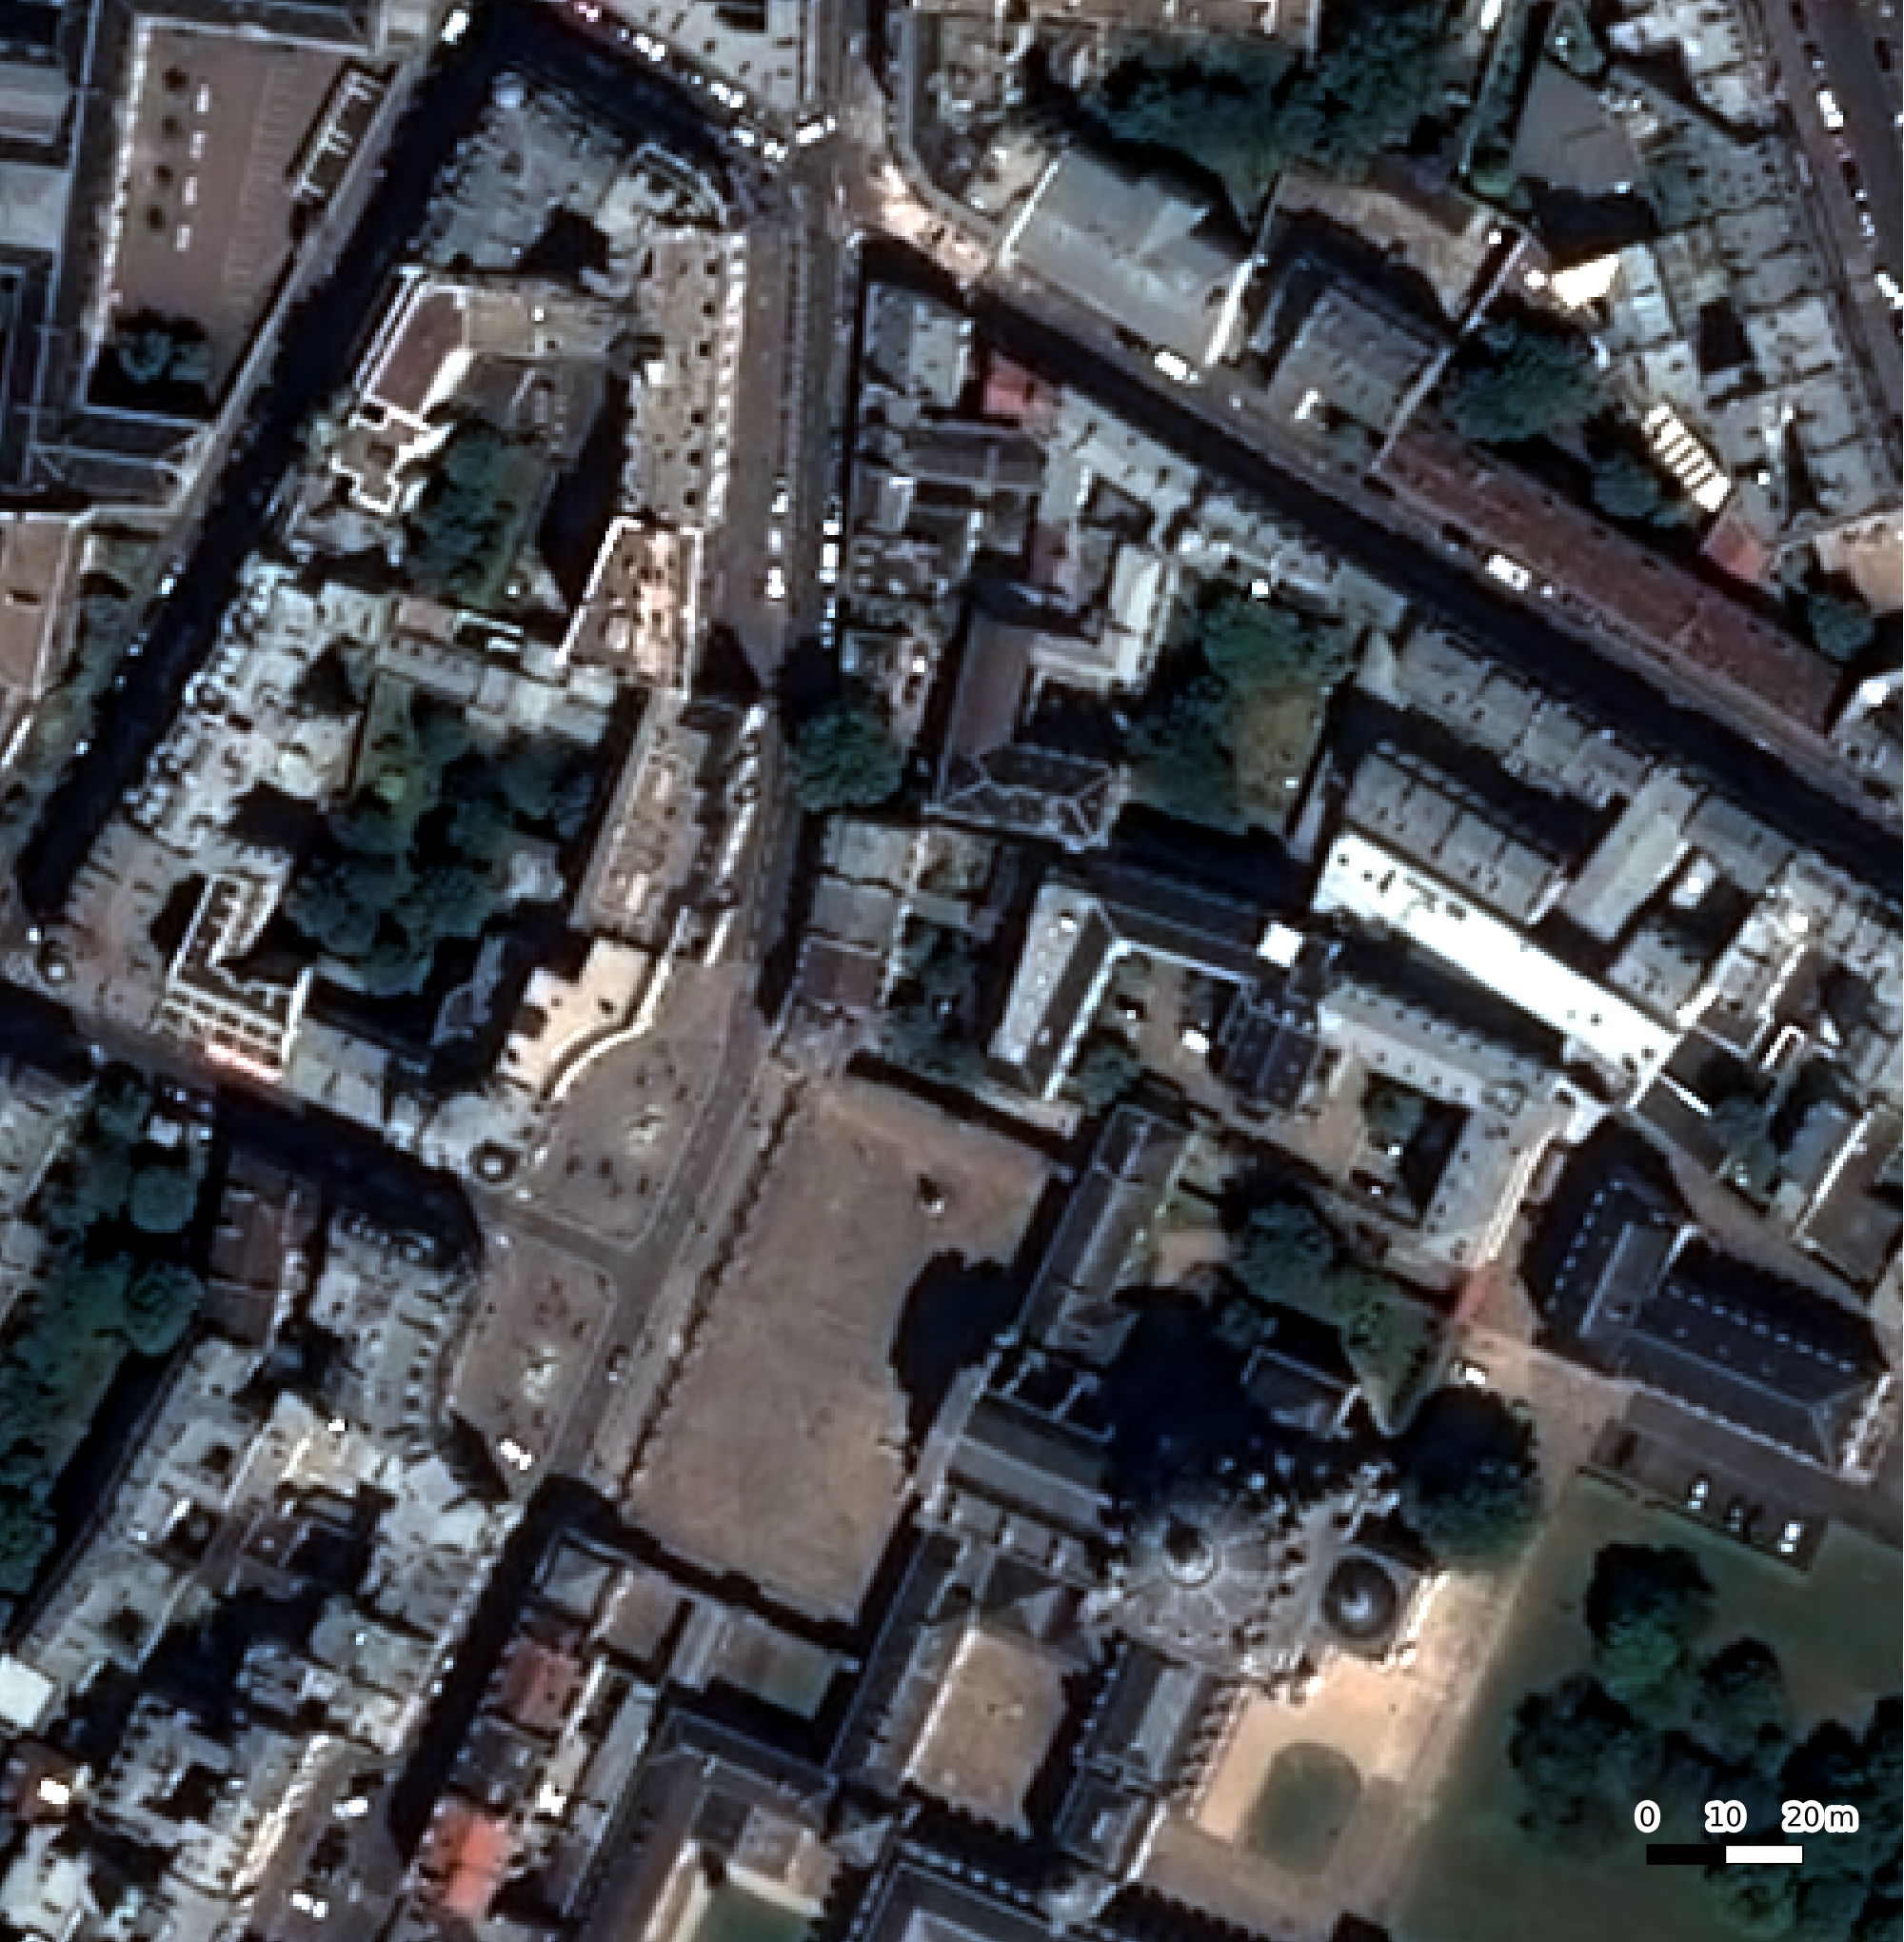
\includegraphics[height=6cm]{Images/0_Intro/Paris_Ortho.png}
        \caption{Pléiades image \copyright \acrshort{cnes} 2017, Distribution AIRBUS DS}
        \label{fig:VDG_ortho}
    \end{subfigure}\hfill
    \begin{subfigure}[t]{0.5\linewidth}
        \centering
        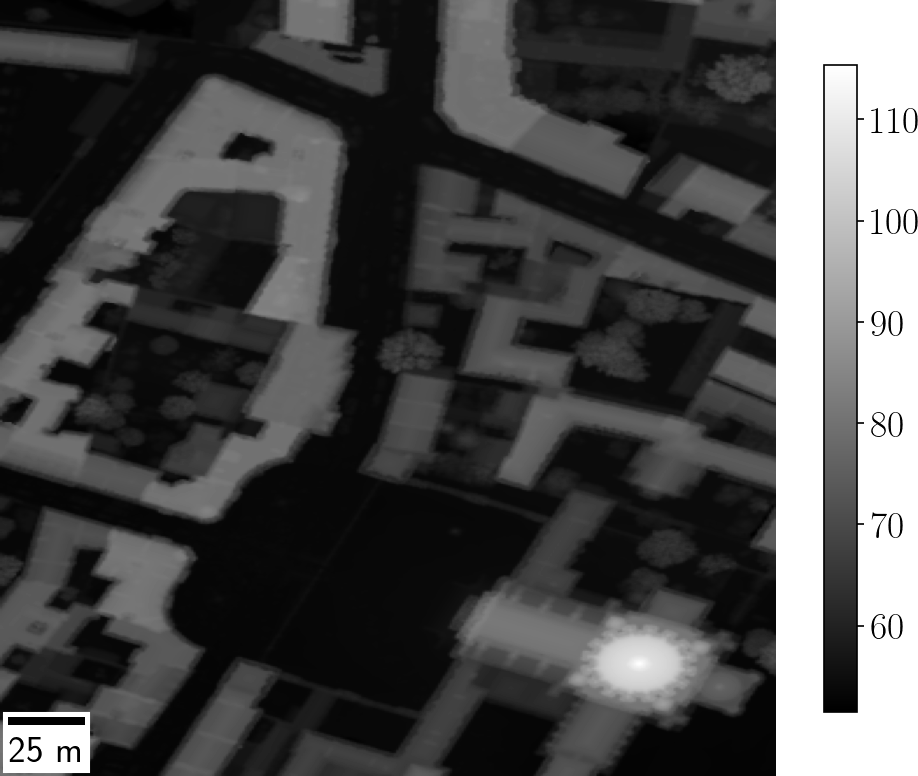
\includegraphics[height=6cm]{Images/0_Intro/Paris_DSM.png}
        \caption{Digital Surface Model from LiDAR HD (unit: m)}
        \label{fig:VDG_dsm}
    \end{subfigure}
    \caption{Satellite image over Val-de-Grâce, Paris at $0.5$m of resolution, and a \acrshort{dsm} over the same area.}
    \label{fig:intro_dsm_example}
\end{figure}

There are multiple ways of creating a \acrshort{dsm} from airborne sensors such as planes, drones or satellites. The first way is to use \acrshort{radar} interferometry, as done by Sentinel-1 satellites \cite{geudtner_sentinel-1_2014}, the Shuttle Radar Topography Mission (SRTM) \cite{farr_shuttle_2007} or TanDEM-X (\cite{krieger_tandem-x_2007}). Typical planimetric resolutions obtained are in the range of a dozen meters (10m for TanDEM-X or 30m for the SRTM). Another method is to construct \acrshort{dsm} by means of stereophotogrammetry \cite{tao_comprehensive_2001}, \ie the science of recovering 3D information from optical images. For this method, images of a scene are acquired from different points of view. Depth information is recovered from the parallax effect between images, \ie the fact that objects closer to the sensors present a greater shift between images than objects in the background. This effect is also what allows depth perception in human vision. \Cref{fig:parallax} illustrates the parallax effect, where the top of Eiffel Tower has a greater position shift in both image than its basis. As current optical satellites have a sub-meter resolution, it is possible to massively produce \acrshort{dsm} covering the globe using photogrammetry for a relatively low cost. The altimetric resolution is typically around one meter, although it depends of the different acquisition angles of the satellites. A final method for producing \acrshort{dsm} is to use LiDAR (laser sensors) \cite{khosravipour_generating_2016}. Using LiDAR allows to obtain very good accuracy. For instance, the french institute IGN (\textit{Institut national de l'information Géographique et forestière}) is using LiDAR to cover the french territory, with a planimetric accuracy of 25 centimeters, and an altimetric resolution of 5 centimeters allowing to observe very small objects. Acquisitions campaigns such as this one are carried out using airborne vehicles, and are thus costly and take a lot of time. Therefore, photogrammetry \acrshort{dsm}s are currently the best solution to produce \acrshort{dsm}s covering the globe  with a sub-meter resolution for relatively low costs. This thesis will therefore mainly considered \acrshort{dsm}s produced using stereophotogrammetry.

\begin{figure}
    \begin{subfigure}[t]{0.32\linewidth}
        \flushleft
        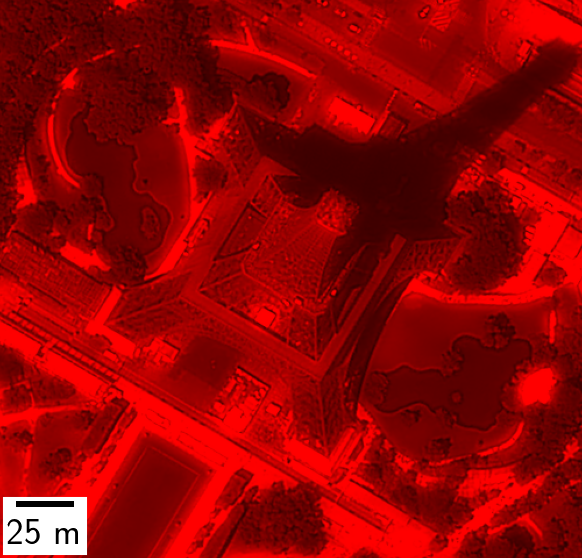
\includegraphics[width=\linewidth]{Images/0_Intro/eiffel_tower_left.png}
        \caption{Left Image (Red channel)}
        \label{fig:eiffel_tower_left}
    \end{subfigure}\hfill
    \begin{subfigure}[t]{0.32\linewidth}
        \centering
        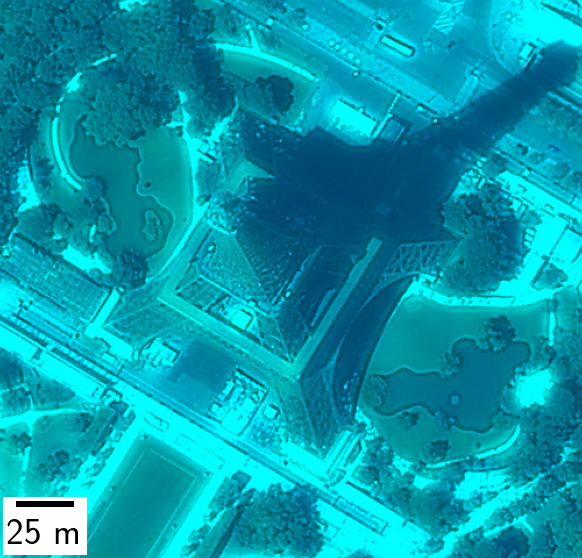
\includegraphics[width=\linewidth]{Images/0_Intro/eiffel_tower_right.png}
        \caption{Right Image (Blue and Green channel)}
        \label{fig:eiffel_tower_right}
    \end{subfigure}\hfill
    \begin{subfigure}[t]{0.32\linewidth}
        \flushright
        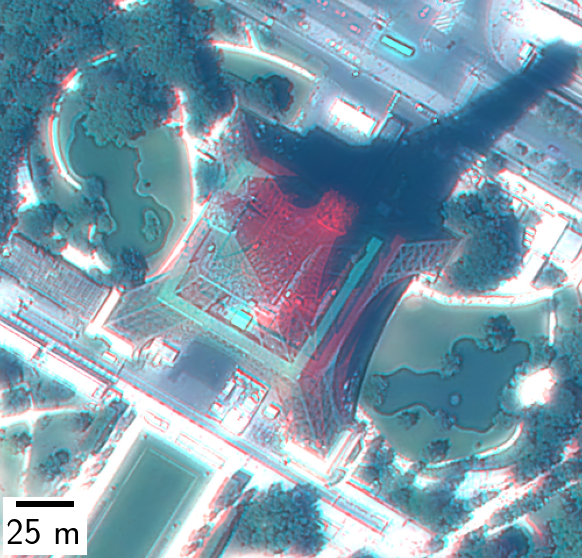
\includegraphics[width=\linewidth]{Images/0_Intro/eiffel_tower_ana.png}
        \caption{Anaglyph}
        \label{fig:eiffel_tower_ana}
    \end{subfigure}
    \caption{Example of the parallax effect: the top of the Eiffel Tower has a greater shift in-between images than its basis. The anaglyph contains the red band of the left image and the green and blue bands of the right image. (Pléiades © \acrshort{cnes} 2023, Distribution AIRBUS DS)}
    \label{fig:parallax}
\end{figure}


In this context, \acrshort{cnes} - the French Space Agency - is planning to launch 4 low-cost optical satellites with Airbus Defense and Space, in order to massively produce \acrshort{dsm} using stereophotogrammetry. This mission, named \acrshort{co3d} (for \textit{Constellation Optique 3D}, \cite{melet_co3d_2020}), was conceived jointly with IGN to provide high resolution \acrshort{dsm} over the globe, at a $50cm$ resolution.

For thus purpose, \acrshort{cnes} developed a pipeline dedicated to process all images provided by the \acrshort{co3d} satellites automatically and at a very large scale. This pipeline is called CARS (``Chaine Automatique de Restitution par Stéréoscopie''), and is composed of many different image processing steps. The different steps will be detailed in the first chapter, but can be summarized as follows:
\begin{itemize}
    \item Resampling of image in a convenient geometry for matching pixels
    \item Dense matching of every pixel between stereo images
    \item Triangulation of matched pixels into 3D points
    \item Rasterization, \ie projection of the 3D points onto a regular grid, therefore yielding the final \acrshort{dsm} 
\end{itemize}
The hardest and most crucial part of this pipeline is the dense matching of pixels. It is also a famous problem in computer vision, which find applications in robotics and autonomous cars for instance \cite{geiger_vision_2013}. Alongside the \acrshort{dsm} computation, one of the requirements of the \acrshort{co3d} mission is to produce a performance map indicating the estimated quality of each cell of the \acrshort{dsm}. This motivates \acrshort{cnes} to lead research in order to estimate the uncertainty amongst the CARS pipeline. The main objective of this thesis is therefore to characterize and propagate the uncertainty throughout this photogrammetry pipeline. Considering the complexity of the \acrshort{cars} pipeline, as well as the time constraint resulting from the future launch of the \acrshort{co3d} satellites, we mainly focus on characterizing the uncertainty of the dense matching step. After quantifying this uncertainty, we propagate it to the end of the pipeline onto the final \acrshort{dsm}.

Characterizing and quantifying uncertainty has many benefits, although it can sometimes be computationally expensive to deal with. It indeed provides additional information for better decision making and risk management. It can also allow for a better understanding of the underlying processes at stake regarding the value of interest. In many cases, uncertainty estimation is treated as a secondary objective in applications. However, jointly estimating a value and its uncertainty can lead to new strategies to reduce the uncertainty or sometimes even improve the performances of the main applications \cite{chen_learning_2023,jiang_unsupervised_2024}.

Before delving into uncertainty estimation and its propagation, we first need to specify what we mean by uncertainty. Uncertainty is a situation where a measure or value of interest is not known, or not known with precision. It is subject to change, as additional information, measures or a different acquisition protocol may reduce how uncertain a value is. It can also be subjective. For instance, someone may be uncertain about the launch date of \acrshort{co3d} satellites, while someone else working at the launch pad might have the answer. This highlights the fact that while everyone has an understanding of what uncertainty is, it encompasses very different concepts in nature. It is common to differentiate the various types of uncertainty by dividing it into two categories: stochastic uncertainty (also called random uncertainty) and epistemic uncertainty \cite{hora_aleatory_1996,frank_treatment_1999}.

Stochastic uncertainty refers to every situation of purely aleatoric nature. For instance, the result of a coin throw, random noise on a CCD captor or the Brownian movement of a particle. An operator typically encounters this kind of uncertainty in a situation where they have access to many measures or observations of the same value of interest. It is usually modeled mathematically with a frequentist approach, using probability measures such as the uniform distribution, Gaussian distribution or the Student's $t$ distribution.

On the other hand, epistemic uncertainty refers to a situation where the value of interest is not known or ill-known due to a lack of knowledge. Think of the previous example with the launch date of satellites, or if someone was asked to guess Io's mass, one of the moons of Jupiter. There is no random process at stake here, and there is usually no point of acquiring multiple samples of the measure if we have a reliable and precise sensor. Once the value of interest is known, the uncertainty no longer exists. It has been proposed to model this kind of uncertainty using a Bayesian approach for probability, by opposition with the frequentist approach. Probabilities here represent a state of knowledge, or degree of belief, one has over the value of interest. It can be updated with additional knowledge, thus leading to the notion of prior and posterior probabilities. We will see during this thesis that other model can be used to characterize this uncertainty, for instance \textit{imprecise probabilities} and more specifically \textit{possibility distributions}. In satellite imagery, those models have been used to detect land changes \cite{lesniewska-choquet_specialite_2020} for instance.

During this thesis, we contributed both to the field of photogrammetry and to the field of imprecise probabilities. Here is a quick overview of the contents that can be found in the following chapters:
\begin{itemize}
    \item \Cref{chap:stereophotogrammetry} introduces the different stereophotogrammetry concepts considered in this thesis. It focuses on the stereo pipeline developed by \acrshort{cnes} and its sources of uncertainty, which will be considered in our applications.
    \item \Cref{chap:representation_of_uncertainty} will introduce the different uncertainty models considered in this thesis, mainly possibility distributions and copulas.
    \item In \Cref{chap:joining_credal_sets}, we propose different methods for creating specific multivariate uncertainty models based on the models introduced in \Cref{chap:representation_of_uncertainty}. We also study the relationships between the methods we introduced.
    \item \Cref{chap:propagating} uses the concepts of \Cref{chap:representation_of_uncertainty} and the results of \Cref{chap:joining_credal_sets} to propagate uncertainties modeled by possibility distributions in a part of the dense matching step of the stereo pipeline.
    \item \Cref{chap:epistemic_uncertainty} also uses possibility distributions, but this time to characterize the uncertainty of the dense matching step itself. Using this method, we are able to obtain confidence intervals at the end of the dense matching step. 
    \item \Cref{chap:elevation_intervals} propagates the disparity intervals to the end of the pipeline, in the form of elevation intervals on the final \acrshort{dsm}. 
\end{itemize}

As our contributions concern two distinct fields of research, multivariate uncertainty and photogrammetry, readers with a level of expertise in one field might be less interested in the second field. We tried, as much as possible, to write each chapter so it can be read and followed by everyone, although some details might need additional knowledge in a field of expertise. To help readers to navigate through chapters according to their center of interests, here is an attempt to classify each chapter into its field of research.
\begin{itemize}
    \item \Cref{chap:stereophotogrammetry} focuses on stereophotogrammetry.
    \item \Cref{chap:representation_of_uncertainty,chap:joining_credal_sets} focuses on the modelling of uncertainty, with \Cref{chap:joining_credal_sets} delving into more advanced concepts.
    \item \Cref{chap:propagating} joins both fields, but leans a bit more towards uncertainty propagation than towards photogrammetry. 
    \item \Cref{chap:epistemic_uncertainty,chap:elevation_intervals} also attempt to join both fields of research, but focuses almost completely on photogrammetry.
\end{itemize}

The rest of this section lists the contributions and research events that occurred during this thesis.
\noindent National conferences:
\begin{itemize}
    \item LFA 2022: ``Copules, probabilités inférieures et ensembles aléatoires : comment et quand les appliquer ?''  \cite{malinowski_copules_2022}
\end{itemize}
International conferences:
\begin{itemize}
    \item SMPS 2022: ``Copulas, Lower Probabilities and Random Sets: How and When to Apply Them?'' - \cite{malinowski_copulas_2022}
    \item ISIPTA 2023 (Special jury recognition Award): ``Uncertainty Propagation using Copulas in a 3D Stereo Matching Pipeline'' -  \cite{malinowski_uncertainty_2023}
    \item IGARSS 2024: ``Robust Confidence Intervals For Digital Surface Models Using Satellite Photogrammetry'' -  \cite{malinowski_robust_2024}
\end{itemize}
International journals:
\begin{itemize}
    \item International Journal of Approximate Reasoning: ``Uncertainty propagation in stereo matching using copulas'' -  \cite{malinowski_uncertainty_2024}
\end{itemize}
Not yet published pre-print:
\begin{itemize}
    \item Available on ArXiv: ``Robust Confidence Intervals in Stereo Matching using Possibility Theory'' - \cite{malinowski_robust_2024-1}
\end{itemize}
Workshops, poster sessions:
\begin{itemize}
    \item Belief 2022 conference: Poster presentation "Using Copulas with Random Sets"
    \item Workshop Imagin ``journée imprécision et incertitude en analyse et traitement d'images'': Funding of the event and communication, and oral presentation ``Uncertainty Propagation in Dense Matching''
    \item SFPT ``Pléiades Neo: de nouveaux satellites pour de nouveaux usages''. Oral presentation: ``Confidence Intervals for Digital Surface Models''
    \item GdR IASIS ``Télédétection et Climat''. Oral presentation ``Estimation d'Incertitudes dans la Création de Modèles Numériques de Surface issus d'Imagerie Spatiale''
\end{itemize}

\pagebreak


\chapter{Introduction to Stereophotogrammetry}\label{chap:stereophotogrammetry}
\section{Digital Surface Models}\commanue{Là c'est en reprendre car tu as copié collé ce paragraphe dans l'intro donc à voir comment tu équilibres entre l'intro et ici. Ici il faudra plus détailler. Dans l'intro tu te limites à expliquer brivèevemnt un DSM, la différence avec un DTM (juste le sol), les différentes méthodes possibles avec leur niveau de résolution et le niveu de détail. Ici tu peux pousser la comparaison, tu peux montrer les différentes produits. Peut-être ici donner des exemples montrer une ville, genre toulouse,  avec différents DSM pour voir les différents niveaux de détails, parler des formats etc. Tu peux aussi parler de l'étendue spatiale des produits, de leur mise à jour. Pour l'instant pas mal d'interventions manuelles.}
\todoroman{Utiliser les slides de formation CARS pour montrer les différentes méthodes pour faire de la 3D, mettre des exmples de LiDAR ou faire un schéma ?}

\commanue{Il faudrait aussi montrer des résultats, en gros c'est quoi en fait un modèle 3D. Après parmi tous les exemples d'utilisation de la 3D que tu donnes tu peux en détailler un un peu plus. Celui que tu préfères.}
Knowing the Earth's topography is crucial for modern geosciences. As such, \acrfull{dsm}, which are a representation of a surface's elevation on a regular grid, appear as a natural solution in many \acrfull{gis}. Indeed, they can easily be handled and provide georeferenced information regarding the topography of an area. \acrshort{dsm} find usage in various contexts for a wide range of applications. In \acrfull{eo} for instance, \acrshort{dsm} are used to monitor changes in vegetation \cite{sadeghi_canopy_2016}, melting rates of glaciers \cite{berthier_glacier_2014, rieg_pleiades_2018}, volcanos \cite{ganci_data_2022}, snow or water resources \cite{marti_mapping_2016, gascoin_theia_2019, yamazaki_merit_2019} \etc Similarly, \acrshort{dsm} are employed for catastrophe management, to predict the potential damage caused by earthquakes or floods \cite{jenkins_physics-based_2023} \dots \acrshort{dsm} are also crucial for ortho-rectifying image, \ie geometrically correcting the effects of distortions between the sensor and the terrain. This process creates a planimetric image with a consistent scale in all parts of the image. It allows images to be easily used in \acrshort{gis} or as background for maps. In urban settings, high resolution \acrshort{dsm} can help drone navigation for Defense applications, or more broadly for urban planning \cite{velazco_3d_2012}.

Nowadays, \acrshort{dsm} are mostly generated from laser scanning with LiDAR sensors, radar interferometry or stereophotogrammetry \cite{youssefi_cars_2020}. Air-borne laser scanning results in \acrfull{vhr} models, but the swath width and cost of acquisition campaigns do not allow to periodically cover the globe\commanue{Pour le LIDAR tu peux citer le Liadr HD de l'IGN: durée de la campagne et données déjà disponible pour montrer que rien que pour avoir la France cela prend beaucoup de temps.}. Space-borne \acrshort{lidar} is mostly used for atmospheric measurements, or discrete measurements \cite{fouladinejad_history_2019}. For instance, NASA's ICESat-2 \cite{jasinski_atlasicesat-2_2020} measures elevation of seas and glaciers using 6 lasers taking measurements along track, which is not adapted for reconstructing high-accuracy DSM. Space-borne radar interferometry remains widely used, and has allowed to create a worldwide digital model of emerged surfaces of the Earth at $30$m and $90$m resolution with the SRTM mission \cite{farr_shuttle_2007}\commanue{Tu peux aussi citer le DEM Copernicus https://spacedata.copernicus.eu/collections/copernicus-digital-elevation-model il faudrait détailler comment il est réalisé. Le SRTM c'est la classe car c'est via la navette Endeavour. Pour revenir au DEM copernicus, il est réalisé à partir de Tandem-X qui est un SAR qui permet de réaliser des DEM jusqu'à 10 à 12m. En fonction du temps tu peux détailler un peu le principe d'acquisitions}. To obtain coarser resolutions\commanue{Donne des ordres de grandeurs qu'on vise par rapport aux autres technos}, it is possible to leverage the technological advancement of optical sensors in orbit to create sub-meter \acrshort{dsm} using stereophotogrammetry with relatively low cost\commanue{Peut-être détailler pourquoi c'est plus low cost}. However, this process is more complex than laser measurements as it deduces height from the principle of parallax. Stereophotogrammetry pipelines usually consists in multiple processing steps with intermediary products (see \ref{sec:classical_stero_pipeline}), with different methods, parameterization and post-processes available for each step (\eg matching, filtering \etc). This broad range of solutions allow to adapt our processes to the type of images and terrain observed, but it sometimes makes it difficult to determine the configuration producing the best quality DSM, or to single out a general good-working configuration. 

This thesis focuses on \acrshort{dsm} obtained from stereophotogrammetry, however we will use \acrshort{dsm} obtained from air-borne LiDAR acquisitions as references to validate our results, considering their high resolutions\commanue{Dans cette section tu mentionnes rapidement le lidar. Je pense que tu dois détailler un peu plus car c'est comme même ta vérité terrain. Il faadrait parler de l'acquisition, du format (points), de la rasterisation (on se retrouve avec plusieurs bandes). Il faudrait aussi citer le lidarHD de l'IGN car c'est vraiment cela que tu utilises comme VT. Tu peux mettre en perspective le temps nécessaire pour faire les acquisitions et mettre à dispo les produits. Notamment cela te sera utile quand tu aborderas la mission CO3D}.
\commanu{ pas plus que manue sur cette section, complètement d'accord}
\todoroman{Schema de \acrshort{dsm} par avion LiDAR, satellite interfero et stereo}
\section{CO3D mission and Pléiades Satellites}\label{sec:co3d}\commanue{Moi je mettrais un titre plus générique sur les satellites optiques haute résolution. Tu démarres par DSM dans la section précédente et tu mentionnes ce type de satellites pour créer des DSM. Donc section suivantes tu parles de ces satellites que l'on peut utiliser pour faire de la 3D (ah transition !) car ils possèdent des atouts : haute résolution, agilité. Tu peux mentionner ensuite les satellites existants Worldview Pleiades CSO (acquisition push-broom que tu peux introduire si tu veux) et ensuite tu introduis la nouvelle constellation de satellites CO3D matrice de bayer, ils volent en formation donc acquistion synchrone (pour une paire),etc. Te connaissant je ferais des sous-sections par exemple : intro globale sur les sat optiques HR, mission actuelles, mission CO3D, données que tu utilises}\commanu{+1}

The following paragraphs detail satellites characteristics relevant to stereophotogrammetry. It is important to notice that although the sensor used greatly determines the resolution of the final \acrshort{dsm}, it is not the only factor at stake here. The altitude and positions of the satellites are also crucial for the resolution\todoroman{parler de \cite{qin_critical_2019} avec un bon ratio et surtout la diff d'angles solaires}, and can be characterized by the \acrfull{b/h} ratio, as in \Cref{fig:RPC}. This ratio is computed by dividing the distance separating the stereo acquisitions by the altitude of the satellite. It indicates the angle formed between the line of sights originating from the satellites towards an object of the scene. A high \acrshort{b/h} allows for high elevation accuracy, but possesses more occluded regions (for instance a narrow street between two high buildings), and conversely for a low B/H \cite{delon_small_2007}.

The main source of images used in this thesis comes from Pléiades images\commanue{Tu peux mentionner çà à la fin de la section (tu sais le truc qui s'appelle une conclusion) une fois que tu as présenter les différentes mission et leur caractéristiques. Tu peux dire que bien que les travaux de cette thèse ont pour vocation de servir dans le segment-sol de CO3D en l'absence de donnée CO3D tu as utilisé des données Pléiades qui ont caractérisques assez proches.}. The Pléiades constellation developed by Airbus is composed of two identical satellites, 1A and 1B. The satellites were launched in 2011 and 2012 in an heliosynchronous orbit at $690$km, for both civilian and defense usages. They provide panchromatic images at a resolution of $70$cm (resampled at $50$cm), and RGB-NIR images at a resolution of $2$m, with a $20$km swath (\url{https://dinamis.data-terra.org/pleiades/}). Their high agility and revisit rate allow them to capture stereo and tri-stereo images for any location on the globe, ideal to produce \acrshort{dsm} with high accuracy\commanue{Il y a même un mode vidéo où tu prends plus d'une dizaine images}. The \acrshort{b/h} ratio for stereo acquisitions can vary between $0.1$ and $0.4$. However, stereo acquisitions is not the only objective of this mission, even though the demand for those products is increasing \cite{berthier_glacier_2014, poli_radiometric_2015, rieg_pleiades_2018, loghin_potential_2020}. The acquisition of stereo images is thus provided on command, which can conflict with other usages of the satellite, and can become costly when trying to cover large areas \commanue{Tu peux mentionner que c'est un satellite dual donc militaire et civil et que les militaires ont la priorité. Après tu peux aussi dire que Pléiades est utilisé lors de l'activation de la chartre https://disasterscharter.org/fr/web/guest/home. Alors on a pas déclenché la chartre mais pour le glissment de terrain dans le sud-est Pléiades avait pris de stéréo.}.  
\begin{figure}
    \centering
    \begin{subfigure}[t]{0.5\linewidth}
        \centering
        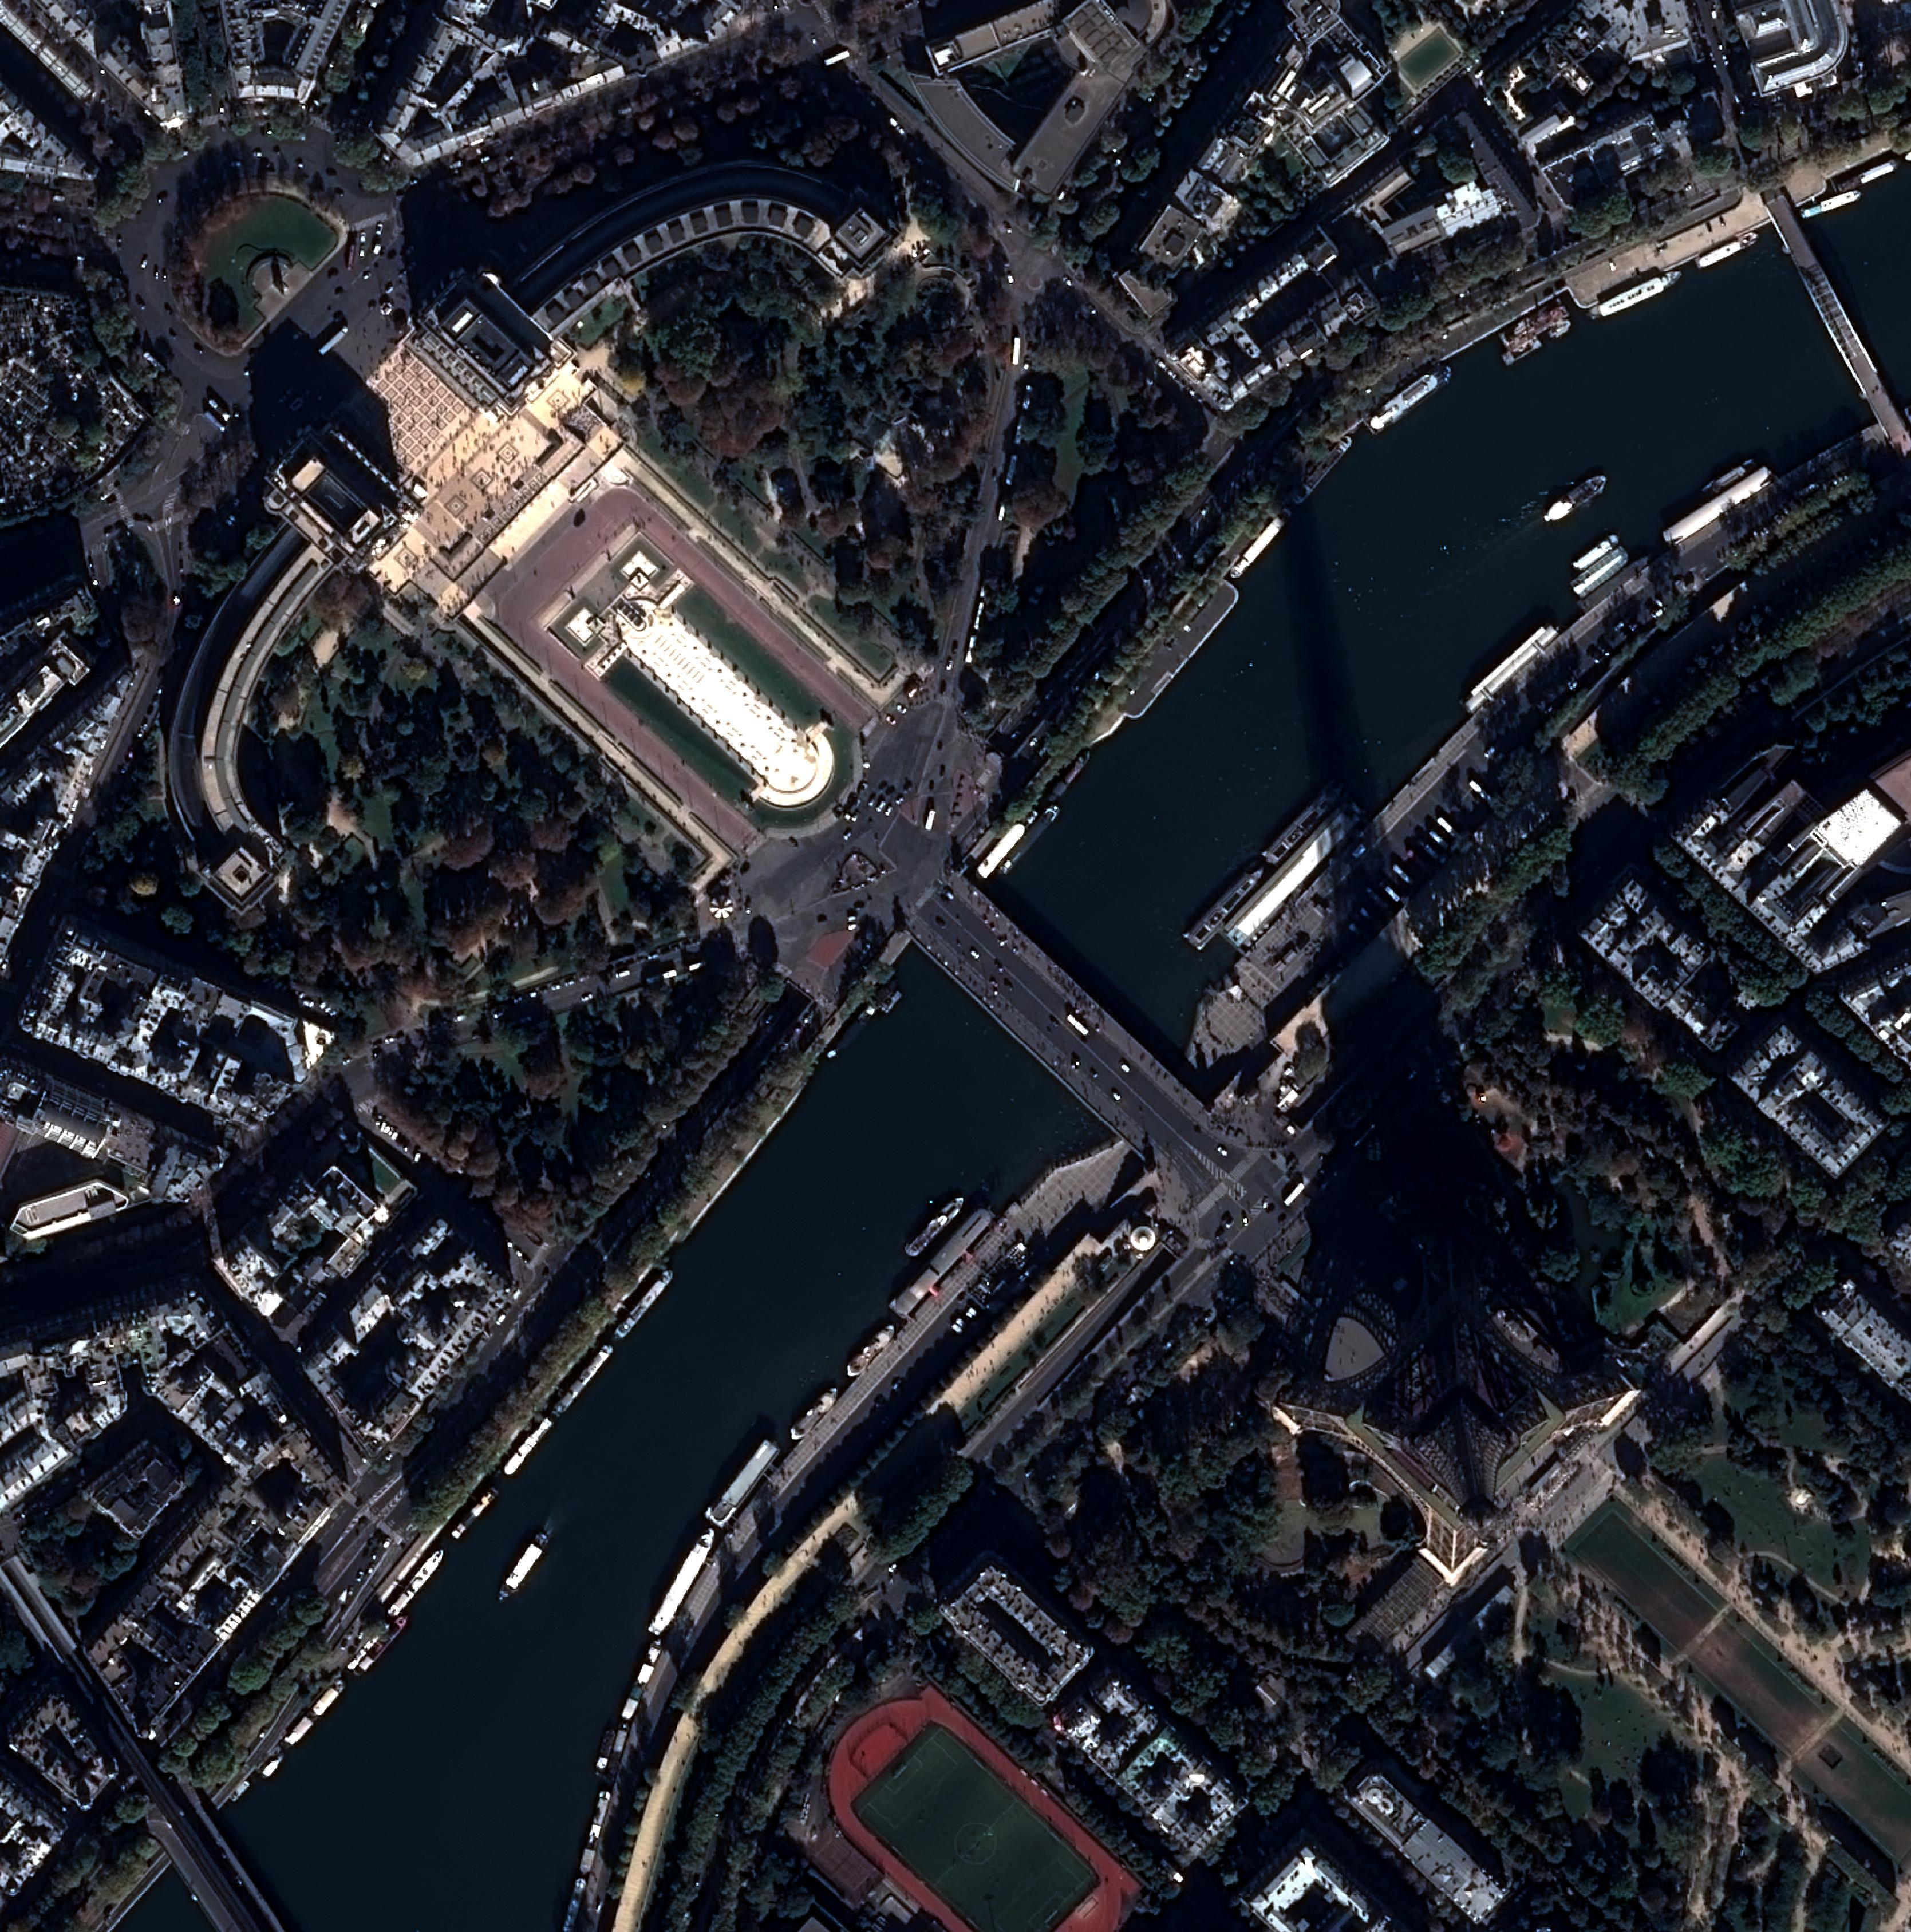
\includegraphics[height=6cm]{Images/Chap_1/Paris_003.jpeg}
        \caption{$14/10/2017$ $11:03:003$}
        \label{fig:Pleiade_over_Paris_a}
    \end{subfigure}\hfill
    \begin{subfigure}[t]{0.5\linewidth}
        \centering
        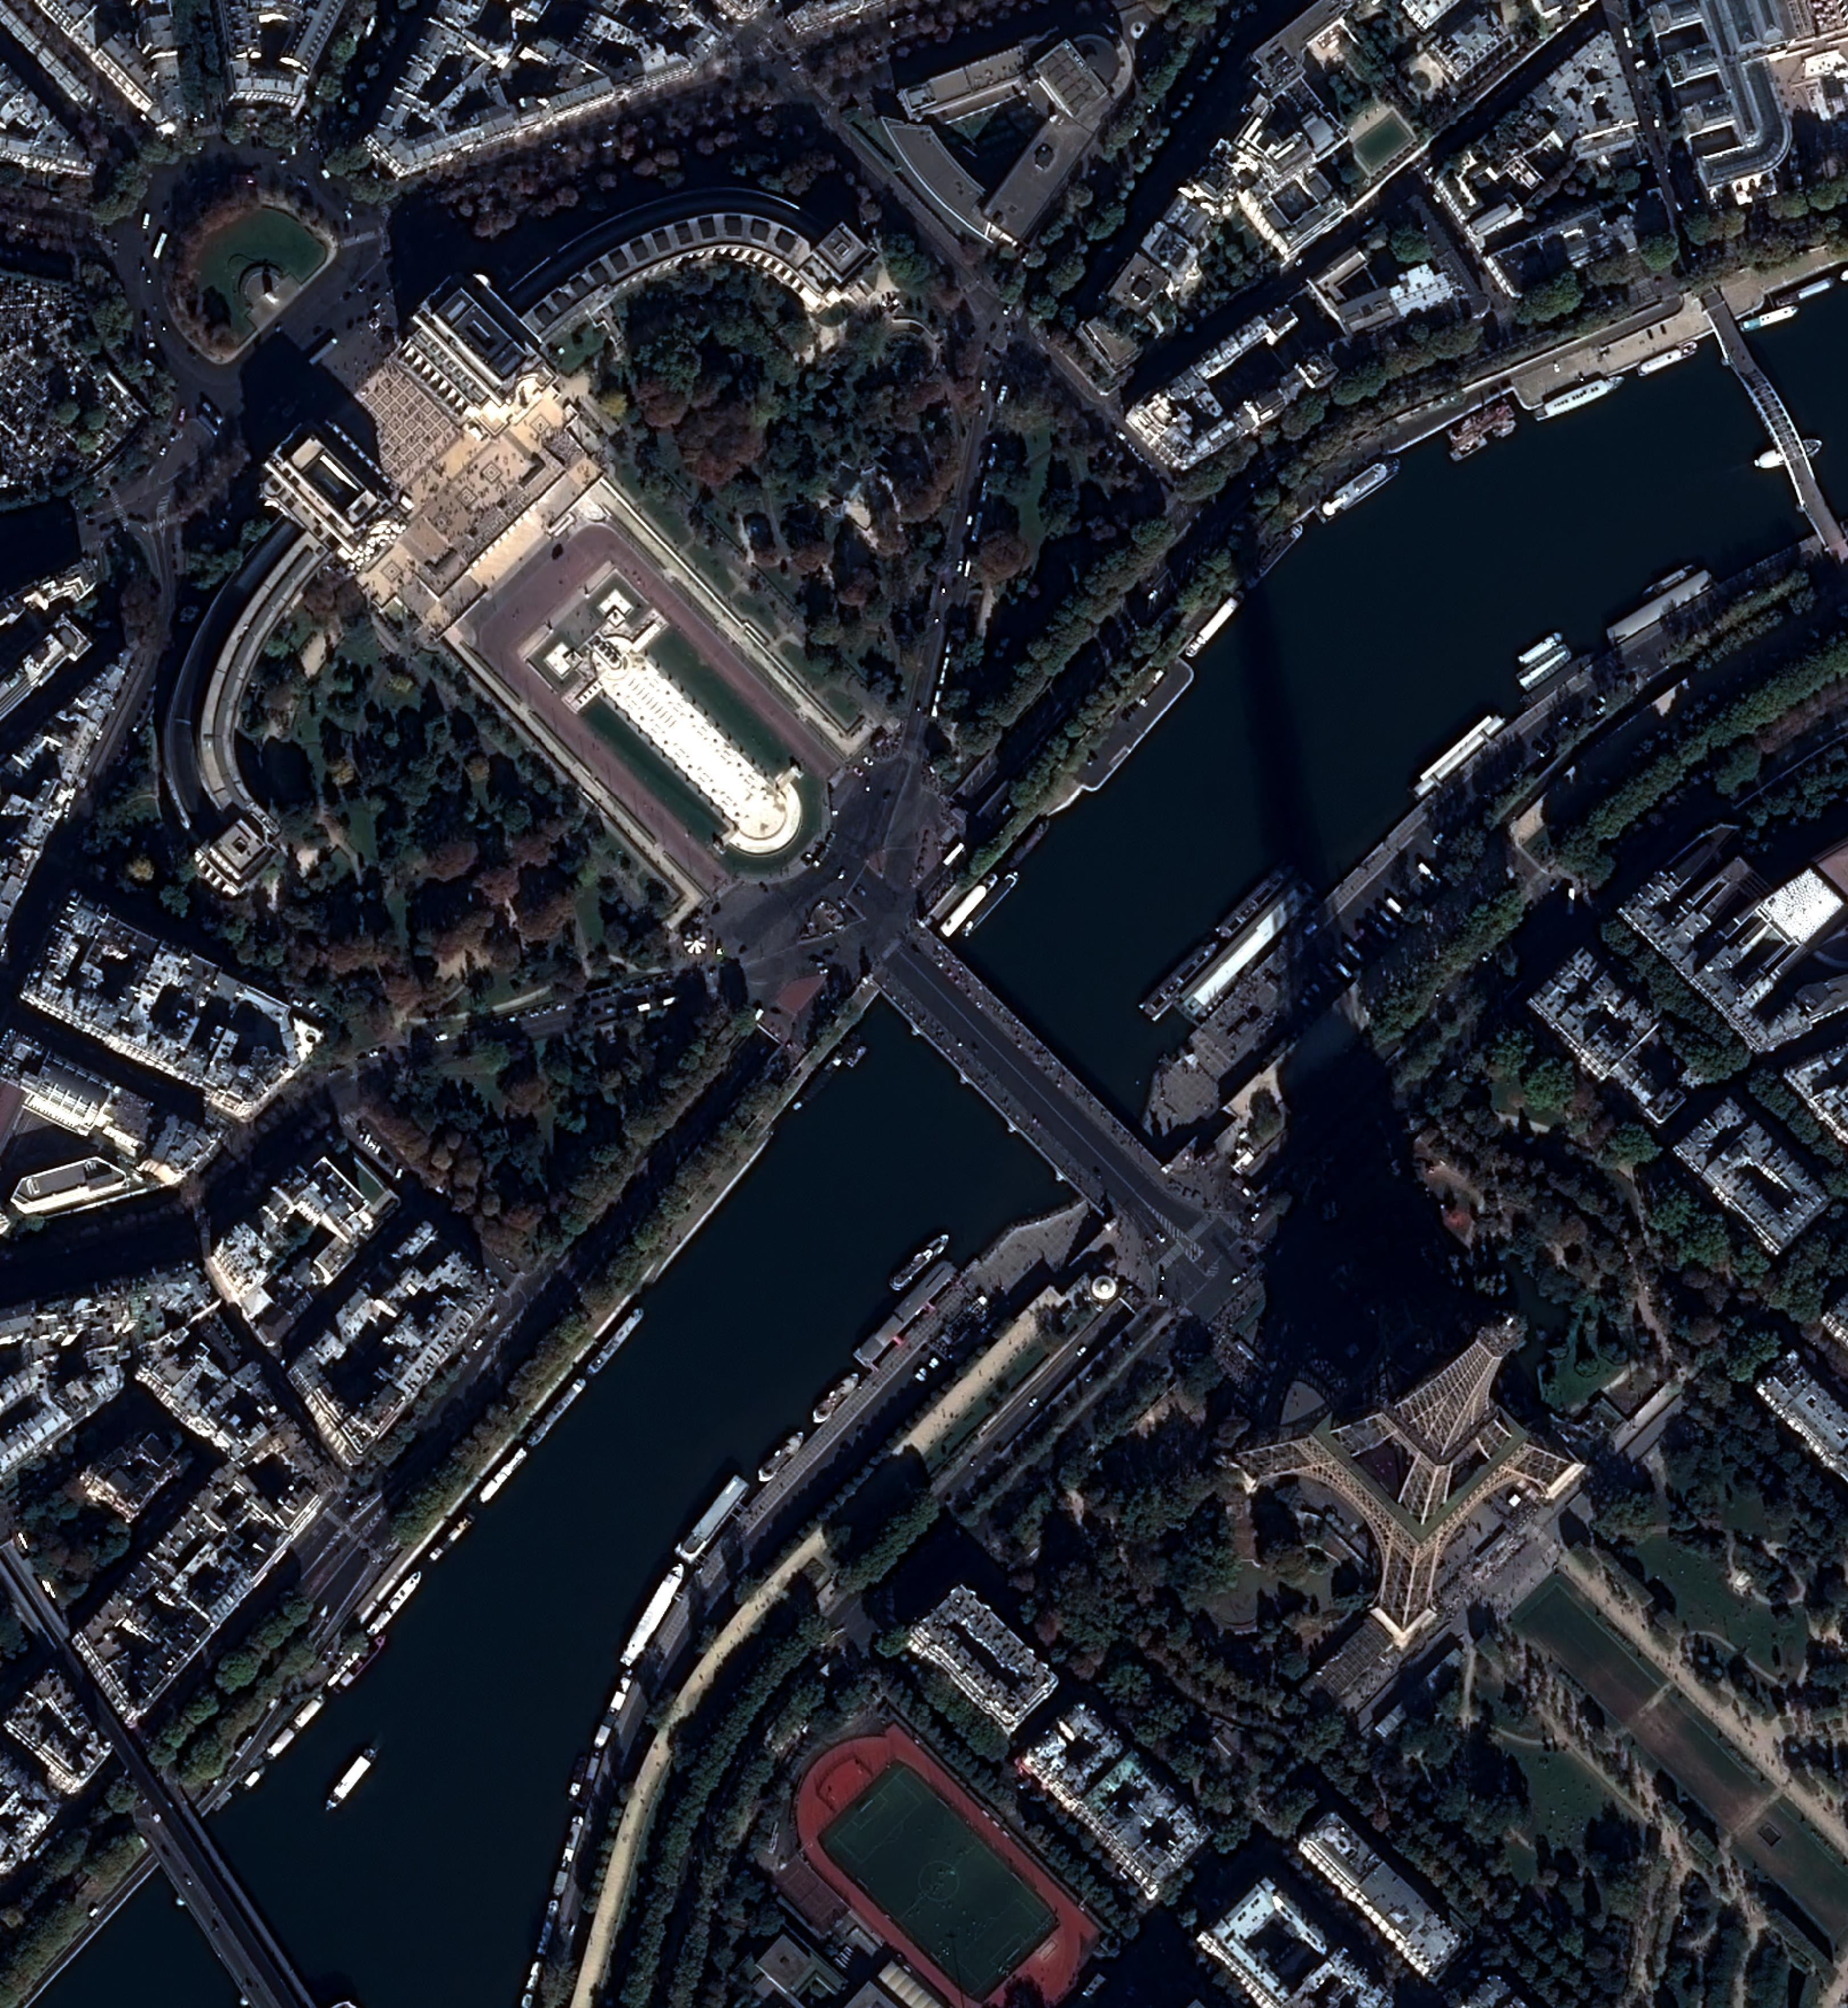
\includegraphics[height=6cm]{Images/Chap_1/Paris_403.jpeg}
        \caption{$14/10/2017$ $11:03:403$}
        \label{fig:Pleiade_over_Paris_b}
    \end{subfigure}
    \caption{Pansharpened Pléiades stereo images over Paris at $0.5$m of resolution. Pléiades \copyright CNES 2017, Distribution AIRBUS DS}
    \label{fig:Pleiade_over_Paris}
\end{figure}

In order to produce a worldwide \acrshort{dsm} with $1$m resolution by 2025, the \acrfull{cnes} is launching the \acrfull{co3d} mission \cite{melet_co3d_2020}. Composed of two pairs of low-cost satellites equipped with \acrshort{vhr} optical sensors, the mission will produce image in the \acrshort{rgb} and \acrshort{nir} spectrum at $0.5$m of resolution \cite{lebegue_co3d_2020}. The pairing of satellites allows for \textit{almost} simultaneous stereo image acquisition, cutting short the transient object problem (\ie objects moving/disappearing between stereo images). To be able to process the amount of data provided by the CO3D mission ($40\,000$ images a day, at $50cm$ resolution and covering a footprint of $7km\times5km$ \cite{melet_co3d_2020, lebegue_co3d_2020}), every step of the pipeline has been developed to be highly parallelizable\commanu{scalable ? to be scalable -> passer à l'échelle. plus large que juste le calcul parallèle qui est une facette de l'optim}. Different acquisition schemes can also be used, such as the video mode, or even the `diamond' geometry acquisition, which acquires a quadri-stereo over a couple of days. Depending on the relief of the terrain observed, the \acrshort{b/h} ratio will be between $0.2$ and $0.3$\commanue{Détaille un peu dans les paysages naturels, les satellites s'éloignent pour augmenter le B/H et dans les zones urbaines ils se rapprochent pour limiter les occlusions}. In parallel with image quality specifications, the CO3D products need to abide to a height accuracy of $1$m on low slopes \comloic{à vérifier je crois que c'est 1m en relatif à CE90. En absolu je ne sais plus}. Another requirement, which is particularly relevant in the context of this thesis, is the production of a performance map supporting the output \acrshort{dsm}. Investigating sources and propagation of the uncertainty inside a 3D stereo pipeline can be beneficial for this performance map requirement\commanue{Je dirais plutôt In addition, the project plans to produce a performance map supporting the output DSM. Therefore, investigating sources and propagation of the uncertainty inside a 3D stereo pipeline is essential for the implementation of this performance map.}\commanu{idem que manue avec juste investigating uncertainty inside a 3D stereo... serait plus direct, tu parles des sources et propagation ailleurs, pas besoin de compliquer la phrase}. 
\todoroman{Dire qu'on est partis du besoin utilisateur pour faire notre méthode et pas l'inverse.}\commanue{Effectivement tu peux expliquer que pour répondre à ce besoin de créer une carte de performance, il existe plusieusr approches. On pourrait faire comme ce qui est fait dans les autres produits (attention c'est à vérifier sur les sites de l'IGN et du DEM coppernicus par ex) il y a une carte qui indiquent une classe de confiance dans le résultat. C'est souvent un masque avec des flags de qualité qui permet de dire si le traitement c'est bien passé ou non. Toi tu as choisi une optique différente en demandant aux utilisateurs quelle information d'incertitude ils attendaient. Et ensuite blabla tu connais l'histoire comme moi.}\commanu{+1}
\todoroman{Parler de Maxar avec les Worldview ?}\commanu{tu peux juste citer mais pas obligé, tu t'en sers pas...}

\todoroman{Schema de la mission CO3D. Type of sensor, push-broom vs raster for CO3D. Pour info c'est une matrice de Bayer}

\begin{remark}
    When an image is acquired both in panchromatic and RGB mode, it is possible to leverage the high resolution of the panchromatic image to improve that of the color image. This fusion technique is called \textit{pansharpening} \cite{loncan_hyperspectral_2015}. We use this technique for clarity in figures and other illustrations of this thesis. It is important to remember that the processed images are the panchromatic images, and not the pansharpened ones which are only used for the final visualization.\commanue{Pour CO3D c'est un peu différent car matrice de Bayer.}
\end{remark} 
\commanu{je sais pas si besoin de cette remarque panchro RGB ici, peut etre quand tu l'utilises plus tard ?, tu verras à la relecture finale. et oui attention différent sur CO3D}

\section{Sensors and Geolocation}\label{sec:sensors_rpc}\commanue{là la transition avec cette partie est plus complexe. Peut-être que je mettrais les éléménts concernant les différents capteurs dans le paragraphe précédent lorsque tu présentes les satellites. Et je déplacerais la partie géoloc dans le pipeline par ex dans une section au début (que tu n'as pas qui explique le niveau de produit que l'on utilise pour faire de la 3D donc image en géométrie capteur avec un modèle de prise de vue où tu peux expliquer que dans ton cas c'est un RPC car le comprimis entre précision et facilité d'utilisation est acceptable.)}
Different types of sensors can be used to acquire satellite images. Below is detailed a (non-exhaustive) list of sensors of interest \cite{cnes_imagerie_2008}

\textbf{CCD matrix sensor}. CDD are classical sensors used, for instance, in current digital cameras. They possess multiple advantages, such as good geometrical quality as all pixels are acquired simultaneously, or the possibility to perform many acquisitions with various angles possible. However, CCD sensors with small pixel sizes are technologically difficult to built. Augmenting the number of pixels complicates the shutter function\commanue{et ça prend de la place. Alors que qq lignes pour un push-broom c'est plus compact}, and requires more radiometric calibration as one pixel equals one sensor\commanue{là je ne suis pas sure de comprendre la remarque}. It is also more complex to acquire long segments of an image \commanue{il faut peut-être expliqué que le satllite est toujours en mouvement donc là tu dois faire en sorte de ralentir (façon de parler car en réalité le satellite qui pivote pour fixer la zone à aquérir suffisamment longtemps pour avoir assez de petits photons)}. CO3D satellites will use this technology\commanue{moi je mettrais cela dans la description de CO3D}.

\textbf{Push-broom sensor}. Those image sensors are only composed of a single cell row, acquiring simultaneously radiometric information alongside a line perpendicular to the direction of the satellite\commanue{peut-être précise que dans ce cas on utilise la vitesse de défilement du satellite}. As only one line of cells is needed, push-broom sensors are simple systems which can capture images continuously, while guarantying good geometrical quality along the rows of the images. A variation of those sensors are TDI sensors (Time Delay Integration). Those sensors function as a push-broom except that each row has the ability to transfer its photon charges to the next row. This allows to capture signals over a longer period of time,  thus reducing the signal-to-noise ratio. Harder to produce, TDI sensors also require a precise control of the satellite so that observed objects stay within a column of the TDI sensor. They are used in Pléiades satellites for instance\commanue{je remonterais cette partie quand tu décris les capteurs HR actuellement en vol.}.

\todoroman{Regarder "Developement and Implementation of Rational Polynomial Coefficient Algorithms for Georeferencing Cartosat-1 Data", et "Metric Information Extraction from Spot Images and the Role of Polynomial Mapping Functions" de Baltsavias et Stallmann}
\commanue{Comme mentionner précédement je mettrais cela plus loin quand tu décris le pipeline CARS. Je ferais une section dédiée sur le fait que CARS prend en entrée une image en géométrie capteur avec un modèle de prise de vue. Si tu veux tu peux préciser qu'il s'agit d'une image où les bandes sont recalées entre elles. Tu peux expliquer à quoi correspond un pixel. On est pas sur une image géoréférence comme on pourrait utiliser dans un SIG. Et ensuite c'est parti pour le modèle de prise de vue... }\commanu{d'accord avec ca}A crucial part of satellite imagery is the ability to perform georeferencement, or georegistratation, of every pixel, \ie, locate their coordinates in an Earth system of coordinates such as latitude and longitude. Physical models possess high geolocation accuracy, but are sensor-specific and are computationally complex. For stereo reconstruction,  generalized sensor models are preferred. Specifically, we will focus on \acrfull{rpc} \cite{grodecki_ikonos_2001} used by the \acrshort{co3d} and Pléiades satellites, and provided alongside images. Sometimes called Polynomial Mapping Functions \cite{baltsavias_metric_1992} or Rational Function Models \cite{tao_comprehensive_2001}, \acrshort{rpc} are functions allowing to transform a pixel's ground location $(X,Y,Z)$ into its image coordinates $(row, col)$. \acrshort{rpc} encode lines of sight of the satellite, \ie the line joining the center of the sensor's cell to the ground and going through the optical center of the sensor. To improve numerical stability and minimize computation errors, the image coordinates and ground coordinates are normalized between $-1$ and $1$, using their scale factors $SF$ and mean values:
\begin{eqnarray*}
    SF_X &=& \max(X_\mathrm{max}-\overline{X},~\overline{X}-X_\mathrm{min})\\
    \Tilde{X}&=&\frac{X-\overline{X}}{SF_X}
\end{eqnarray*}
The same processed is applied to $Y,Z,row$ and $col$. To avoid heavy notation in this section, we will refer to every normalized coordinate using their non-normalized symbol.

\begin{figure}
    \centering
    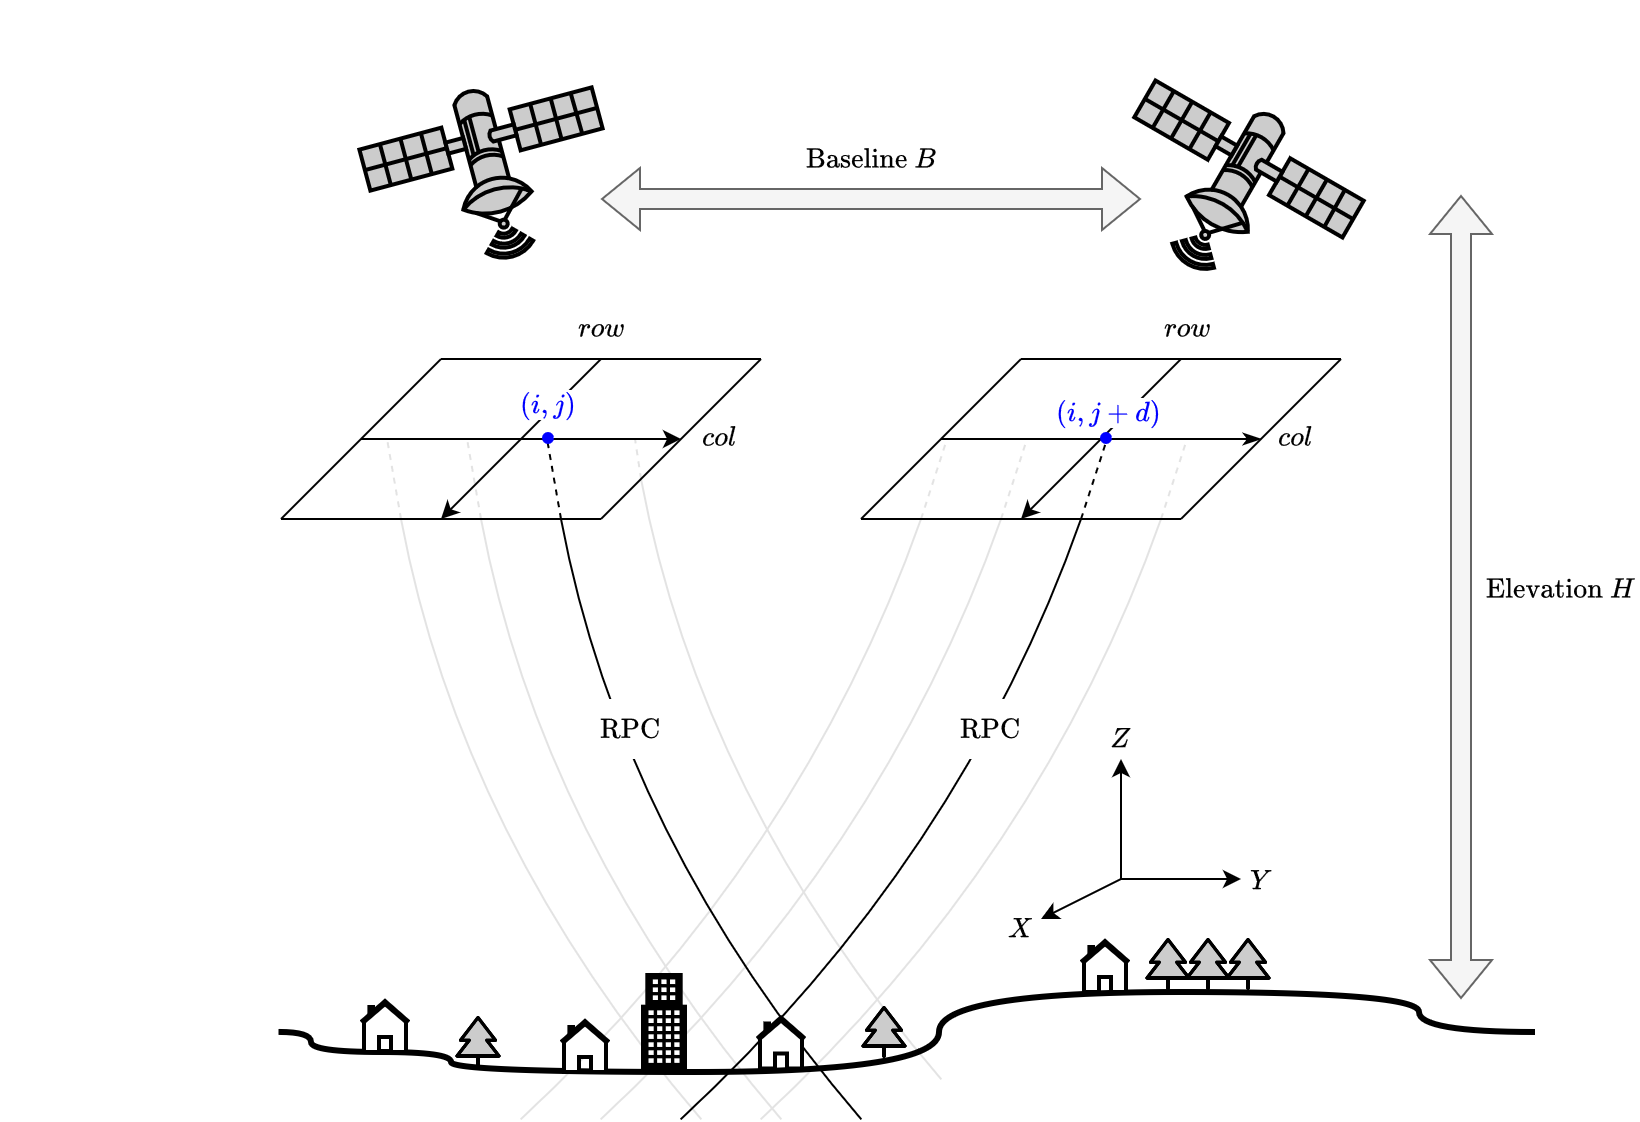
\includegraphics[width=0.8\linewidth]{Images/Chap_1/RPC.png}
    \caption{Triangulation of the position of a point using RPC models}
    \label{fig:RPC}
\end{figure}

Formally, \acrshort{rpc} are defined as rational fractions of polynomials:  
\begin{eqnarray}
    \RPC:\mathbb{R}^3 &\rightarrow&\mathbb{R}^2\nonumber\\
    (X,Y,Z) 	&\mapsto& \left(\frac{Num_{row}(X,Y,Z)}{Den_{row}(X,Y,Z)}, \frac{Num_{col}(X,Y,Z)}{Den_{col}(X,Y,Z)}\right)\nonumber\\
    &\mapsto&(row,col)\label{eq:rpc}
\end{eqnarray}
where $Num_{row},~Den_{row},~Num_{col}$ and $Den_{col}$ are the numerators and denominators for rows and columns respectively, expressed as polynomials with a maximum order of $3$:
\begin{eqnarray*}
    Num_{row}(X,Y,Z) &=& \sum_{i=0}^3~\sum_{j=0}^{3-i}~\sum_{k=0}^{3-i-j}a_{ijk}X^iY^jZ^k\\
    &=& a_{000} + a_{100} X + a_{010} Y + a_{001} Z + a_{110} XY + a_{101} XZ \\
    &&+ a_{011} YZ + a_{200} X^2 + a_{020} Y^2 + a_{002} Z^2 + a_{111} XYZ \\
    && + a_{210} X^2Y + a_{201} X^2Z + a_{120} XY^2 + a_{102} XZ^2\\
    && + a_{021} Y^2Z + a_{012} YZ^2 + a_{300} X^3 + a_{030} Y^3 + a_{003} Z^3
\end{eqnarray*}
$Den_{row},~Num_{col}$ and $Den_{col}$ respectively possess different coefficients $a_{ijk}$. The order or indexing of $a_{ijk}$ may differ in the literature. For instance, they can be numbered from $0$ to $19$ or $1$ to $20$, and do not refer to the same indeterminate. \acrshort{rpc} are computed using reference ground control points.\commanue{Discute avec Daniel mais tu peux effectivement utiliser des poinst de contrôle pour fitter les ceoff mais dans le cas des segments-sols, ils utilisent le modèle physique et ensuite ils fittent sur ce modèle un modèle RPC pour les utilisateurs normaux.}

It has been showed in \cite{baltsavias_metric_1992} that RPC are well suited to be used for ortho-rectification and stereophotogrammetry, as they possess good accuracy and are computationally fast. For stereo photogrammetry, it is ofter required to use the inverse \acrshort{rpc} model. As \acrshort{rpc} encode a line of sight given an image coordinate, the use of an additional elevation coordinate is required to move from the image space to the object space (\ie to go from a 2D space to a 3D space). It can be a geoid modelling the Earth's surface, or a \acrshort{dsm} with higher resolution. Knowing the true elevation $Z$ of a pixel, we define the inverse model as:
\begin{eqnarray}
    \RPC^{-1}:\mathbb{R}^3 &\rightarrow&\mathbb{R}^3\nonumber\\
    (row, col, Z) 	&\mapsto& (X,Y,Z) \label{eq:inverse_rpc}
\end{eqnarray}

An illustration on how RPC are used in stereo-photogrammetry is presented in \Cref{fig:RPC}. \commanu{c'est dommage de pas l'utiliser pour l'étape de triangulation. Ici, l'exemple le plus direct serait juste une loc sur ellipsoid ou DEM, ca evite au lecteur de penser autre chose (exemple image page accueil https://shareloc.readthedocs.io/)}

\section{Structure of the Stereophotogrammetry Pipeline}\label{sec:classical_stero_pipeline}
This section dives more into details of the inner workings of stereophotogrammetry\commanu{soit cohérent tout le long, 1 mot, 2 mots? pas pareil partout (dans l'intro t'as mis 2 mots)}, and presents the stereo pipeline mainly considered in this thesis. Photogrammetry is the science of deducing information from photographic images\commanu{ref ? un livre référence par exemple}. A sub domain of photogrammetry is stereophotogrammetry, which specifically consists in deducing 3D information from multiple photographic images. Although multiple stereophotogrammetry setups can be achieved, for instance using structured light \cite{scharstein_high-accuracy_2003} or different wavelength \cite{geng_rainbow_1996}, we focus here on the pipelines designed for processing satellite images, which are used and studied in this thesis. 

The main idea of stereophotogrammetry for satellite images and other 3D pipelines is to identify the parallax of objects between multiple images, and to deduce the distance between the object and the sensors from this displacement\commanue{Tu as le droit de mettre des schémas en plus tu risques d'en avoir besoin pour ta prez}. When expressed in pixels, the displacement is called disparity\commanue{si tu as un schéma plus loin mets une ref, sinon fait un schéma. C'est important que les termes que tu vas utiliser un nombre incalculable de fois par la suite soient bien définis}. To determine this disparity, the images must first be corrected from atmospheric effects (small clouds, aerosols, \etc) to go from top-of-the-atmosphere radiance to the actual light that illuminates the Earth surface \cite{hagolle_maja_2017}, called reflectance \comloic{je ne sais pas à quel point c'est vrai dans le cas de CO3D. Les acquisitions sont synchrones et le B/H petit. Je serai supris que en TOA les résultats soient très différents mais peut être. En tout cas je n'ai pas en tête de travaux qui le montrent.}\commanue{Alors si CO3D respecte le process standard la correction atmo c'est au niveau 2A donc tes images sont déjà projetées au sol donc on ne fait pas de 3D avec elles. Les images pour faire de la 3D c'est en général ce qu'on appelle de niveau 1B (correction radio et géo (recalage et modèle géométrique). A partir de 1C on projette au sol. Mais à vérifier avec David si CO3D utilise les niveaux de produits standards}. Many stereo setups\commanue{Alors là tu t'éloignes du satellite, je ne sais pas s'il ne faut pas le préciser. Ici quand tu parles de setups c'est les autres applications utilisant la 3D comme les voitures autonomes, les rovers sur Mars que tu as en tête} align their cameras in such a way that objects only move horizontally between images \cite{geiger_are_2012, scharstein_high-resolution_2014, keselman_intel_2017}. This allows to restrict the search space for pixel matches to a single row instead of the whole image. In a way, most people's eyes also present this alignment\commanue{je suis d'accord avec l'analogie mais la transition avec in a way c'est bizarre.}. When operating satellites, it is more complex to ensure that the sensors disposition will stay consistent\commanue{peut-être le tourner différemment, comme tu le mentionnes, habituellement dans les autres applications qui utilisent de la stéréo, les caméras sont montées de telle sorte à être dans la géométrie. Tu fais du principe d'acquisition satellite (qui défile) on n'est pas dans ce cas. C'est pas que c'est plus complexe. C'est que le mode d'acquisition ne le permet pas.}, thus requiring some pre-processing step to rectify images and ensuring that the displacement of an object only occurs horizontally (see \Cref{sec:epipolar_geometry}). Then matching pixels are determined by computing their disparity in a step called stereo matching presented in \Cref{sec:stereo_matching}\commanue{je suis en train de me dire que ce que tu racontes est très liée à la géométrie épipolaire. Mais que dans les faits les pipelines satellites font parfois le choix de reprojeter l'image de droite dans la géométrie de l'image de gauche donc corrélateur 2D car la mise en géométrie épipolaire est complexe. Donc peut-être que dans toute cette partie l'intérêt de la géométrie épipolaire doit être gardé pour plus tard et de rester haut niveau pour l'instant en disant seulement que l'étape consiste à trouver les pixels homologues entre deux images ou même pas car dans cette section, tu te limites à parler d'objets et non pas de pixels}\commanu{je suis d'accord, je ferais plus simple et ferait en 2 fois}. The 3D coordinates of the corresponding object are determined by computing the intersection between matching pixels' lines of sight (or best approximation if they do not strictly intersect). This results in a point cloud, where each point correspond to a match of two pixels\commanue{là on repart sur la notion de pixels donc soit tout ton paragraphe raisonne avec des objets dans les images soit tu parles de pixels dans les images. Mais si tu passes de l'un à l'autre c'est perturbant car les deux notions ne sont pas interchangeables}. The point cloud can be processed to remove outliers, and is then projected into a regular grid to obtain the desired \acrshort{dsm}. The following section dives more into details for the specific case of the CARS stereo pipeline\commanue{bah en fait non, dans la suite tu repars sur les pipelines existants. Donc je mettrais un peu d'ordre. Tu as fait un paragraphe très générique sur ce qu'est un pipeline 3D. Ce que tu as raconté ici, s'applique à tous, ça tombe bien c'est l'intro. Ensuite nouvelle section tu mentionnes les pipelines existants, tu peux fortement t'inspirer de ce que j'avais écrit pour ISPRS pour CARS. Tu auras peut-être besoin de la géometrie épipolaire. Et après tu enchaines sur CARS.}\commanu{en effet, mieux avec 1 général 2 pipeline existant 3 le notre cars, ca cleanera le meme feeling que manue entre ses deux sous sections}.

\subsection{Structure of the Stereo Pipeline}
Several stereo pipelines processing satellite images exist in the literature. We can think of NASA's \textit{ASP} \cite{shean_automated_2016}, IGN's \textit{MicMac} \cite{rupnik_micmac_2017}, Centre Borelli's \textit{s2p} \cite{franchis_automatic_2014}, DLR's \textit{CATENA} \cite{kraus_fully_2013}, Ohio State University's \textit{RSP} and \textit{SETSM} \cite{qin_rpc_2016, noh_surface_2017}\todoroman{Regarder "Metric Evaluation Pipeline for 3D Modeling of Urban Scenes" pour des comparaisons}. All those pipelines roughly possess the same structure, \ie pre-processing, images resampling in a convenient geometry for pixel matching, dense matching, triangulation and rasterization. Variations in those pipelines concern the different preprocessing steps (bundle adjustment, histogram equalization), the type of geometry used, the dense matching algorithms available \etc\commanue{Donc pour un chapitre de thèse va falloir plus détailler, je suis sure que j'ai mis plus d'info dans la publi de CARS ;) Il faudrait ajouter par rapport à ce que j'avais moi, c'est si certains pipelines gèrent ou non les incertitudes. Je n'avais pas regardé ce point à l'époque. Sans parler d'incertitudes, tu as peut-être a minima des flags qualité qui permettent au moins de dire ce résultat-là on regarde même pas}\commanu{et du coup, je découperais: une partie à part état de l'art des satellite stereo pipeline + une partie dédiée sur cars, revoir ta structure pour aider le lecteur} We will focus on the CARS pipeline used in this thesis, developed by CNES \cite{michel_new_2020}. A schematic of the different steps of the pipeline are presented in \Cref{fig:cars_pipeline}.
\todoroman{Insister sur le fait que CARS est tout automatique, y compris sur les cartes de performances à grande echelle. A voir avec Sylvia comment les DEM de l'IGN ont une carte de perf, et si oui si elle est pas manuelle}

\begin{figure}
    \centering
    \includegraphics[width=\linewidth]{Images/Chap_1/CARS_pipeline_detailed.png}
    \caption{Different steps of the CARS pipeline}
    \label{fig:cars_pipeline}
\end{figure}
The CARS pipeline works with grayscale images, but colored images (for instance pansharpened image) can be provided alongside the grayscale image\commanue{alors petite précision, Pandora ne fait de la corrélation que sur une seule bande. Donc CARS en général utilise les images PAN car plus résolues et ensuite complète sa sortie avec des infos issues du RGB. Donc je dirais plutôt que CARS (à cause de l'étape de corrélation) travaille majoritairement en mono-bande. Après si on envisage des étapes où on se sert du RGB par exemple pour faire de la classif ou pour filtrer, on pourrait avoir une plus grande utilisation de l'information provenant de plusieurs bandes}\commanu{je sais pas si c'est central en effet. a la lecture, ca donne l'impression que c'est important alors que c'est un peu annexe: ici tu présentes surtout les grandes étapes et les grandes lignes de fonctionnement du pipeline. La color peut etre un sujet intéressant mais annexe à ta problématique, attention digression comme vu par manue}. The grayscale pixels will be used in the pipeline\commanue{car les PAN sont plus résolues pour les images Pléiades. Pour CO3D on prendrait la bande verte car 2 fois plus de pixels}, but the colorimetric information will be kept until the final DSM, thus providing an ortho-rectified image\commanue{C'est pas faux mais il faut que tu fasses attention à toutes ces petites remarques que tu ajoutes et qui peuvent perdre le lecteur. As-tu besoin de parler les images orto RGB? Si oui, vraiment maintenant ou peut-être au moment de la rasterisation}.\commanue{Donc là voir remarque précédente, mais je mettrais ici clairement ce que c'est que les inputs de CARS : image en géométrie capteur mono-bande avec un modèle de prise de vue.}

\subsection{Resampling in Epipolar Geometry}\label{sec:epipolar_geometry}
The first step of the CARS pipeline is to resample the stereo acquisitions into a convenient geometry to carry out the dense matching\commanue{alors dans l'intro de cette section (qui es utile pour poser les termes), tu n'as jamais dis dense matching. Tu as juste parlé de matching (j'ai vérifié) donc dis juste matching entre les pixels. Tu expliqueras le terme dense dans l'étape de matching à proprement parlé}. This geometry is the epipolar geometry \cite{cnes_imagerie_2008}, which is constructed so that each line of an image follow the movement of the satellite, \ie the objects move only horizontally between the reference and secondary stereo images. This will\comloic{pourquoi will?} greatly facilitates the dense matching\commanue{juste matching} as the search space for a match is only limited to a one dimensional space instead of a two dimensional space around the pixel\comloic{la fin de la phrase est peut être pas utile}. A first approximation\commanue{pourquoi first approximation?} of the epipolar geometry can be computed using the respective geolocation models of both images $\RPC_1$ and $\RPC_2$\comloic{je suis peut être passé trop vite il me semble pas encore avoir croisé les termes RPC, ça vaut le coup d'en toucher un mot}. Indeed, given the altitude $Z$ of the object represented by pixel $(row_1, ~col_1)$ in the reference image, then\comloic{then pas utile} we can deduce its ground location $(X, ~Y, ~Z)$ using $\RPC_1^{-1}$. The position in the secondary image of those coordinates\comloic{là on ne sait pas trop si tu parles de la représentation du pixel (row,col) il y a deux phrases ou de la groud location} can then be retrieved using $\RPC_2$. In short, we found the secondary coordinates $(row_2,~col_2)$ of a pixel $(row_1,~col_1)$ in the reference image given an elevation $Z$\comloic{C'est pas limpide. Je vois comment ça marche dans ma cars mais là en te lisant je suis pas convaincu de l'ordre des opérations / explications}: 
\begin{equation}
    (row_2,~col_2) = \RPC_2\circ\RPC_1^{-1}(row_1, ~col_1, ~Z)\label{eq:epipolar_transfer}
\end{equation}
By varying the altitude in the range of considered elevations $[Z_{min},~Z_{max}]$, $\RPC_2\circ\RPC_1^{-1}$\comloic{tu peux la nommer f2->1 et préciser que c'est la fonction de colocalisation 2 vers 1} provides a characterization of the parallax between images. The lines described by $\RPC_2\circ\RPC_1^{-1}$ are thus the epipolar curves for the reference image\commanue{Tel que tu l'expliques, c'est plutôt la transformée d'une ligne de l'image de gauche par la composition des fonctions de RPC qui te donne la ligne épipolaire correspondante dans l'image de droite. Donc effectivement en faisant ça tu obtiens la ligne dans laquelle faire ta recherche. Mais il faudrait ajouter que c'est juste inutisable dans la pratique. On passerait son temps à faire des locs. Ce qu'on recherche c'est une transformation pour rééchantilloner les images}. Similarly, $\RPC_1\circ\RPC_2^{-1}$ provides the epipolar curves for the secondary. The range of considered elevations $[Z_{min},~Z_{max}]$ can be determined with a low resolution digital elevation model\commanue{pour faire une loc inverse tu as besoin d'une élévation donc n'importe quoi fait l'affaire.}. This is not constraining as a geoid of the Earth can be used, and there also exists open models such as the NASA's SRTM \cite{farr_shuttle_2007} ($30$m and $90$m of resolution between $-56\degree$ and $60\degree$ of latitude), or ESA's Copernicus DEM ($30$m and $90$m of resolution worldwide).  \todoroman{Parler aussi de la RGE Alti de l'IGN. regarder aussi s'ils ont un masque de perf}\commanue{Dans la suite tu repars sur le modèle pinhole. Donc cette partie sur le RPC on a l'impression que c'est pas fini. Peut-être commencé par parler du pinhole. C'est un modèle simple, c'est facile de calculer la transformée en géométrie épipolaire. Le souci c'est que le modèle pinhole n'est pas valide sur toute l'image mais localement. D'où l'utilisation du RPC mais les RPC ne permettent pas une formule analytique. Donc on passe par une grille de transformation. Et on utilise des compositions de fonctions de loc (et pour la fonction inverse on a besoin d'une hauteur).}

\begin{figure}
    \centering
    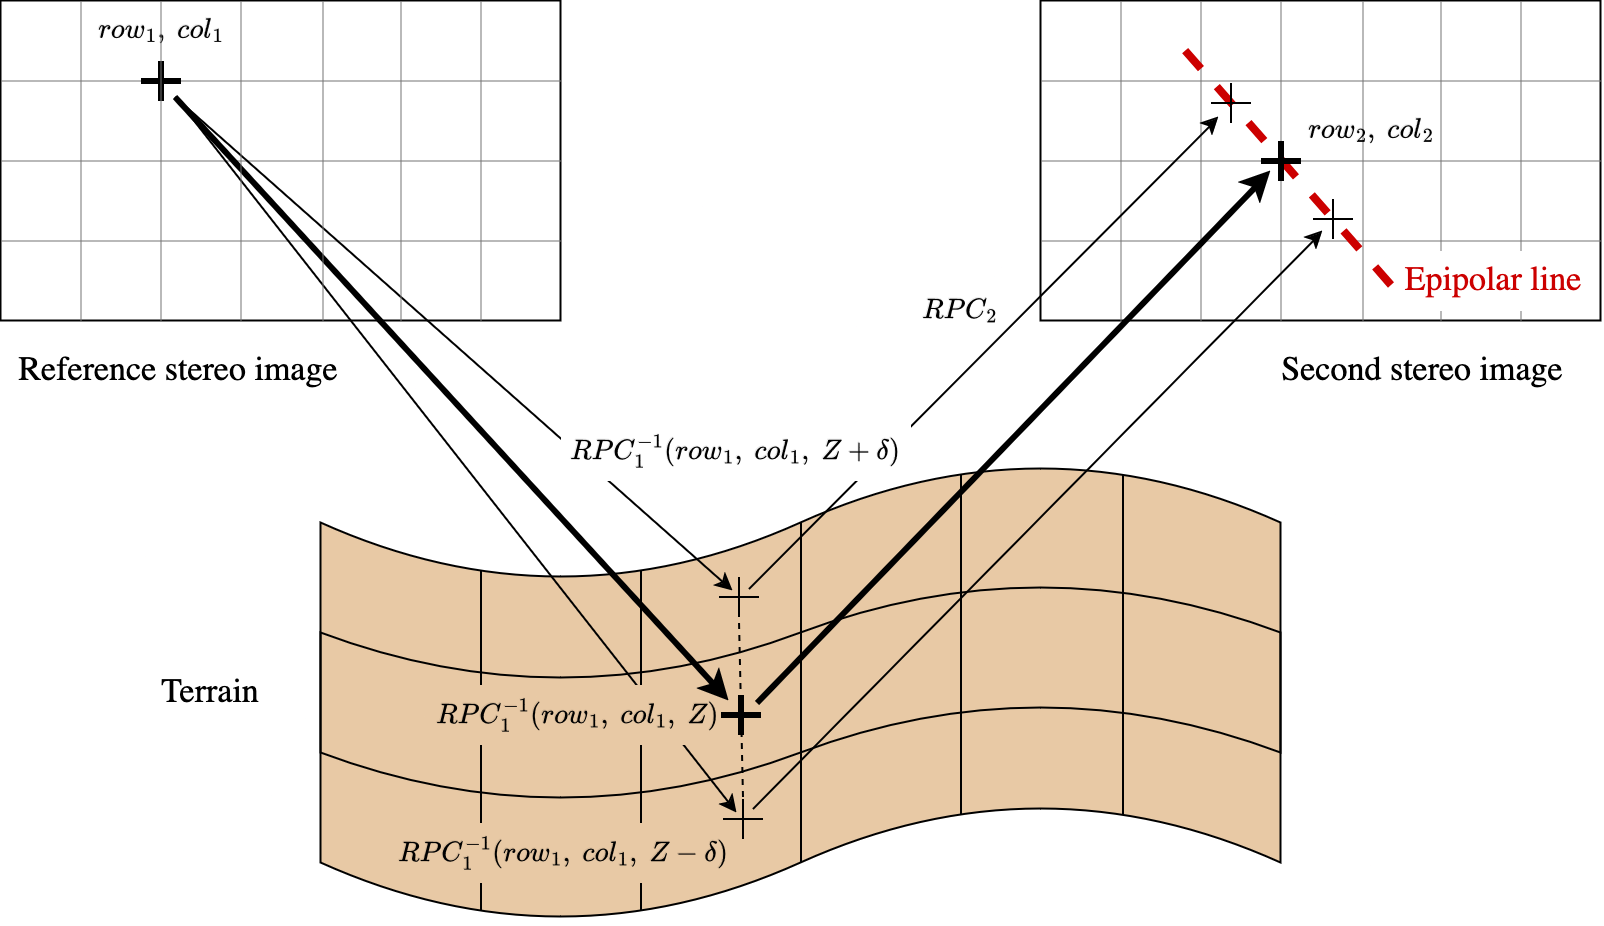
\includegraphics[width=\linewidth]{Images/Chap_1/epipolar_lines.png}
    \caption{Computation of an epipolar line for a pixel using small height variations}
    \label{fig:epipolar_lines}
\end{figure}

Captors using a pinhole camera model have a perfectly defined epipolar geometry, modeled by an affine transform \cite{hartley_multiple_2004}. This not true for push-broom sensors \cite{morgan_epipolar_2004}, but other models exist allowing to compute such a geometry \cite{oh_piecewise_2010, de_franchis_stereo-rectification_2014, koh_unified_2016, michel_new_2020}\commanue{Alors je mettrais la remarque en premier. Si on utilise un modèle simple pour décrire le modèle géométrique donc du pinhole c'est facile de faire le passage en géométrie épipolaire. Le pb c'est que le modèle pinhole n'est pas valide sur l'intégralité de l'image. Donc il faut l'appliquer par morceau, c'est ce que fait S2P. Résultat, tu as des effets de tuilages sur ton image. Ici on cherche une méthode pour passer en géométrie épipolaire en utilisant direct la précision du RPC. Alors tu cites la publi ISPRS de CARS mais justement on ne passe pas par du pinhole}\comloic{je rajouterai que ça va un poil vite. Quand tu dis qu'il existe d'autres modèles pour calculer la géométrie épipolaire tu passes un peu sous silence que ce sont des approximations, et justement la complexité dont on hérite avec des acquisitions de l'espace et des capteurs VHR principalement pushbroom, c'est qu'on ne peut pas exprimer la géométrie épipolaire de façon exacte sur l'ensemble du produit. Ensuite tu cites plusieurs papiers, il est important de noter ce qui distingue CARS des autres et notamment de la référence s2P (réf car IARPA winner tout ça tout ça). Dans s2p on a fait une approximation locale du modèle de caméra par un modèle type pinhole donc on peut réutiliser les algos de la computer vision à l'échelle d'une tuile sous réserve qu'elle soit petite. Dans CARS on cherche une représentation globale que l'on va exprimer par une grille de déformation qui fournit pour chaque point de la géométrie épipolaire sont équivalent dans la géométrie capteur.}. In the CARS pipeline, \cref{eq:epipolar_transfer} is evaluated with an elevation $Z$ extracted from the low resolution elevation model, and for small variations of altitude $Z\pm\delta$\commanue{alors je connais le principe mais là j'avoue que c'est pas clairement précédément tu as dit que tu pouvais avoir la ligne et là tu expliques que tu le fais localement. J'aurais tendance à renverser l'explication. Comme on ne peut pas avoir une trasformation analytique, on recherche une grille et voilà comme on évaluer chaque point de la grille.}. Those three points allow to compute the direction of epipolar lines for every pixel of both images as in \Cref{fig:epipolar_lines}\commanue{C'est un peu rapide. Comme on ne peut pas avoir une transformation en géométrie épiplaire qui peut s'écrire simplement via une transformation matricielle comme pour du pinhole. On décide d'exprimer la transformation par une grille que l'on peut prendre avec un pas assez large vu que les variations sont assez basse fréquence}. This method generates what is called an epipolar grid $g_{e1}$ joining every epipolar coordinate $(row_e, ~col_e)$ to its position in the reference image $(row_1, ~col_1)$:
\begin{align}\label{eq:epipolar_grid}
    g_{e1}(row_e, ~col_e) = (row_1, ~col_1)
\end{align}
A similar grid $g_{e2}$ is determined for the secondary image, which is actually computed jointly with $g_{e1}$. Those grids also use the low resolution elevation model\commanue{l'approche nécessite une altitude pour faire la loc inverse mais tu pourrais utiliser une altitude constante et la technique fonctionnerait. Si on utilise un DSM basse résolution c'est que cela permet de limiter l'intervalle de recherche.} to determine which altitude corresponds to a null disparity\commanue{Moi je tournerais plutôt la phrase qu'avec cette méthode par construction la disparité nulle correspond à l'altitude du DSM utilisé}\comloic{+1, c'est pas construction, tu peux amener ça de façon anecdotique, en gros c'est dans cette géométrie épipolaire là, puisqu'on pourrait en créer une autre, que la disparité nulle correspond à Z, où Z est censé être le Z dont tu parles plus haut et autour duquel tu ajoutes +/- delta, tu pourrais de Zcoarse ou Zdem. Enfin je veux dire, tu parles de Z en disant qu'il est extrait du low resolution elevation model mais on pourrait penser à un scalaire qui aurait au moins une occurence dans le low res elevation model, et peut être qu'il faudrait low res digital elevation model pour garder le lien avec DEM que tu présentes plus haut}. After the dense matching step, a disparity of $0$ would mean that the object has the same altitude than that of the low resolution elevation model. For more details on the way epipolar grids are computed, we refer to \cite{michel_new_2020}. Using those grids, it is possible to resample the reference and secondary images in their respective epipolar geometry. 

Because the geolocation models\comloic{c'est un termes que tu n'utilises que deux fois dans le manuscrit et je dirai qu'on pourrait l'introduire un peu mieux peut être pour ceux qui n'ont pas l'habitude de manipuler des images satellites. Peut être que dans le 1.3 le titre est trop vague, et le contenu fait un peu commercial plus que scientifique par moment. Je pense que tu pourrais y exposer plutôt des notations et des principes un peu originaux pour ceux qui découvrent l'image satellite mais sont qd mm intéressés par la thèse parce que par ailleurs ils font du stereo matching. Par exemple avant de parler des RPCs ou quoi faudrait introduire les systèmes de coordonées peut être. A la limite juste ECEF et UTM mais de quoi faire intervenir les notations X,Y, lon, lat, Z et h et les fixer pour le reste du manuscrit. Et ensuite seulement aborder les modèles géométriques et les RPCs et donc les loc directe et inverse. D'autre part à partir du 1.3 on parle souvent de DEM et d'intersecter un DEM du coup mais on parle pas du référentiel du DEM, en gros le Z du DEM il est par rapport à quoi ? faut faire intervenir géoide et ellipsoide je pense. Ou alors je vais trop loin mais là disons qu'on aborde tout ça très vite dans les premiers sous chapitre de cette section. Ensuite tu peux aborder les modèles de caméra utilisé dans le spatial un peu comme tu le fais mais sans le mélanger avec les RPCs, faudrait structurer avec un chapitre sur les syst de coord, un sur les modèles de caméra, un sur la géo d'acquisition en 3D qd même avec le b/h, avec le termes "nadir" peut être aussi, et ensuite les RPCs ou quoi)}  have a limited precision, there might be a misalignment left in the epipolar grids. To correct this error, a set of SIFT points \cite{lowe_distinctive_2004} is computed between the reference and secondary epipolar images. For every match, the difference between their rows is computed. The secondary epipolar grid is then corrected so that row differences are null on average. Once aligned epipolar grids have been obtained, stereo images can been resampled in epipolar geometry one last time so that \commanu{so that what ? à enlever ou finir la phrase}

\begin{remark}
    By computing the disparity for the set of SIFT points, it is possible to estimate the range of disparities to be considered in the dense matching step for a relatively low computation cost. We will see in \Cref{sec:triangulation} that there is an approximately\comloic{approximation?} allowing to simply convert disparities into an elevation using the $B/H$ ratio presented in \Cref{sec:stereo_matching}. Therefore, an approximation of the elevation of each SIFT match can easily be computed. A low resolution elevation model can then be derived from it, thus removing the need of an external model such as SRTM or Copernicus DEM.\commanue{Je ne suis pas sure que ça doit rester juste une remarque. MOn souci c'est qu'il y a plusieurs infos dans ta remarque. Premièrement les SIFT sont utilisés pour calculer l'intervalle de dispariaté,deuxième on peut convertir la disparité et troisièment on peut faire un DSM endogène. Donc la première partie de la remarque t'es surement utile. Le reste c'est à voir ou il faut faire plusiuers remarque.}\comloic{ouais c'est un paragraphe que tu pourrais avoir écrit la veille de la remise du manuscrit ça ;-) ça fait un peu, j'ai oublié deux trois choses qui rentrent pas dans le moule actuel donc je fais un patch. J'ai entendu dire que quand on fait un patch c'est un pb de conception si c'est pas un pb de temps ^^'}
\end{remark} 

Epipolar grids can also provide a good approximation of the disparity to altitude ratio $d_{alt}$ over the whole image, which can be used to determine the approximate $Z$ resolution of the DSM. It can also convert disparities into height as we will see in \Cref{sec:uncertainty_pandora}\commanue{Alors là je ne suis pas de comprendre le lien direct entre grille épipolaire et disparité}. 

\subsection{Stereo Matching}\label{sec:stereo_matching}
\subsubsection{Different Approaches}\commanu{pas sur que tu aies besoin de ce titre de soussoussection, j'enleverais}
Dense matching\commanue{je pense qu'il faut que tu prennes une phrase pour expliquer pour quoi on parle de dense matching. C'est assez typique de la télédétection où on fait du matching sparse pour recaler et dense pour la 3D. Donc je mentionnerais que l'on parle de dense car on réalise le matching sur l'ensemble de pixels} can be performed once epipolar images have been computed. As stereo matching is an important problem is\commanue{in?} computer vision, multiple algorithms have been proposed to compute a dense disparity match\commanue{c'est bizarre l'association de terme.}. Dense matching algorithms can be broadly classified into two categories: classical approaches following the steps outlined by Scharstein \etal \cite{scharstein_taxonomy_2001}, and deep-learning based methods \cite{laga_survey_2022}.
\begin{remark}
	In the domain of stereo matching, the reference image is often referred to as the \textit{left} image, and the secondary image is the \textit{right} image.
\end{remark}

Recently, deep-learning methods have been greatly improving\commanu{bizarre en anglais, je mettrais have greatly improved, sinon ce serait have been improved mais marche pas} the results of stereo matching algorithms \cite{tosi_survey_2024}\commanue{il faudrait que tu précises, tu parles de la stéréo en général et/ou de la télédétection}. Best results on famous benchmarks have been obtained using 2D an 3D convolution neural networks \cite{guo_openstereo_2024, liu_playing_2024}. Those deep-learning approaches often face generalization challenges, particularly when applied to images that differ from their training datasets. It is especially true in the case of satellite imagery \cite{mari_disparity_2022, jiang_rethinking_2024}, as there is a large variety of landscapes and sensors to consider, landscapes change with the seasons, and radiometry can also vary greatly between two acquisitions\commanue{je me dis que MCCNN c'est du deep learning mais c'est juste une étape donc quand tu parles de méthodes DL tu entends méthodes full DL ou non ? Si c'est le cas il faudrait le préciser.}. Many datasets are available for stereo processing, especially for autonomous cars \cite{geiger_are_2012, geiger_vision_2013}, but it is harder to come across open satellite datasets due to the costs and copyrights of satellite images, even if more datasets tends to be released \cite{bosch_semantic_2018, le_saux_data_2019, huang_urban_2022}\commanue{Les idées sont là mais l'ordre est pas évident. Soit tu expliques que les techniques DL notamment pour les voitures autonomes trustent les meilleurs perfs, car il y a bcp de datasets que la généralisation se passe bien puisqu'au final la structure de l'image varie peu. Et ensuite tu passes à la télédétection et là tu expliques que c'est plus mitig. Même si ces méthodes obtiennent de très bons résultats en télédétection, elles génralisent mal car les paysages sont très voire trop diverses, et en plus la création de VT est difficiles}. Obtaining ground truth data for satellite imagery is also challenging, as airborne campaigns are costly and often need to cover large areas to match satellite acquisitions\commanue{Oui c'est vrai que une acquisition LIDAR est chère. Mais c'est surtout que générer le jeu de données : aligner les données hétérogènes est un enfer et que tenir comptes des différences entre les acquisitions est un casse-tête et aussi passer le lidar en géométrie épipolaire}. All those factors make the training of a performing and generalizable network for satellite imagery quite challenging. Even though deep stereo algorithms will probably end up by replacing cost-based methods in future years\commanu{tu n'en sais rien et ca décrédibilise ton approche de thèse pour rien, donc à tourner plus positivement. Tu montres avant que ce n'est pas du tout sur. donc justifie plutot que l'approche de ta thèse est tout à fait logique et argumenté}, we will not focus on deep end-to-end algorithms\commanue{c'est ici que tu mentionnes le end-to-end} in this thesis and instead restrict ourselves to so-called \textit{classical} methods used in satellite stereo pipelines. Those methods have the advantage of relying on an extensive literature on the subject, and implementing new features (for instance a new optimization strategy or a new cost function) is usually easier and does not require to re-train the whole network\commanue{en même temps MCCNN c'est du DL donc... En fait le truc c'est que les méthodes end-to-end en plus de mal généraliser actuellement (on peut se dire que peut-être ce verrou peut sauter à terme) sont des boîtes noires donc mettre de l'explicabilité comme tu le fais ça me paraît pas être adapté. Il faudrait que le réseau apprenne la disparité et son intervalle d'erreur en même temps. Je pense que cette phrase est à mettre dans le paragraphe suivant.}\comloic{je pense aussi que l'objectif de la thèse rend compliqué l'utilisation d'algo IA end to end. C'est pas seulement landscape et sensors to consider, il y a le b/h, la résolution des images, les angles de dépointages à b/h équivalent etc. et le fait que la plupart de ces algos subissent un entrainement supervisé. Vu qu'on ne sait pas estimer la disp parfaite entre deux images avec des algos non IA (sinon à quoi servirait l'IA) on peut pas générer la VT donc on prend une source exogène qui fait office de VT mais qui présentent des incohérences. Tu peux qd même ouvrir sur le fait que des algos entrainés de façon non supervisée pourraient s'affranchir de certaines problématiques citées mais c'est pas encore mature et c'est pas écolo or CO3D c'est du low cost}.

Classical approaches usually encompass the following steps \commanu{+described in following subsections, pour aider à la transition?} \cite{scharstein_taxonomy_2001}\commanue{je ferais une liste avec item, tu n'es pas limité en nombre de pages.}: matching cost computation, cost aggregation, disparity computation, and disparity refinement. \Cref{fig:stereo_matching_pipeline} illustrates those different steps. In this thesis, we will mainly consider classical approaches\commanue{tu l'as déjà dit dans le paragraphe d'avant.}, specifically as the CARS pipeline uses a dense stereo correlator called Pandora, developed at CNES (\url{https://github.com/CNES/Pandora})\commanue{J'ajouterais une phrase pour dire que maintenant tu vas détailler les étapes}\commanu{et à la lecture des étapes d'après on ne retrouve pas celle de ton schema général, notamment sur SGM pas mis dans le pipeline. Pour quelqu'un qui connait pas trop, c'est confusing. Donc j'introduirais bien les memes étapes "générales" que tu décris après}.

\begin{figure}
	\centering
	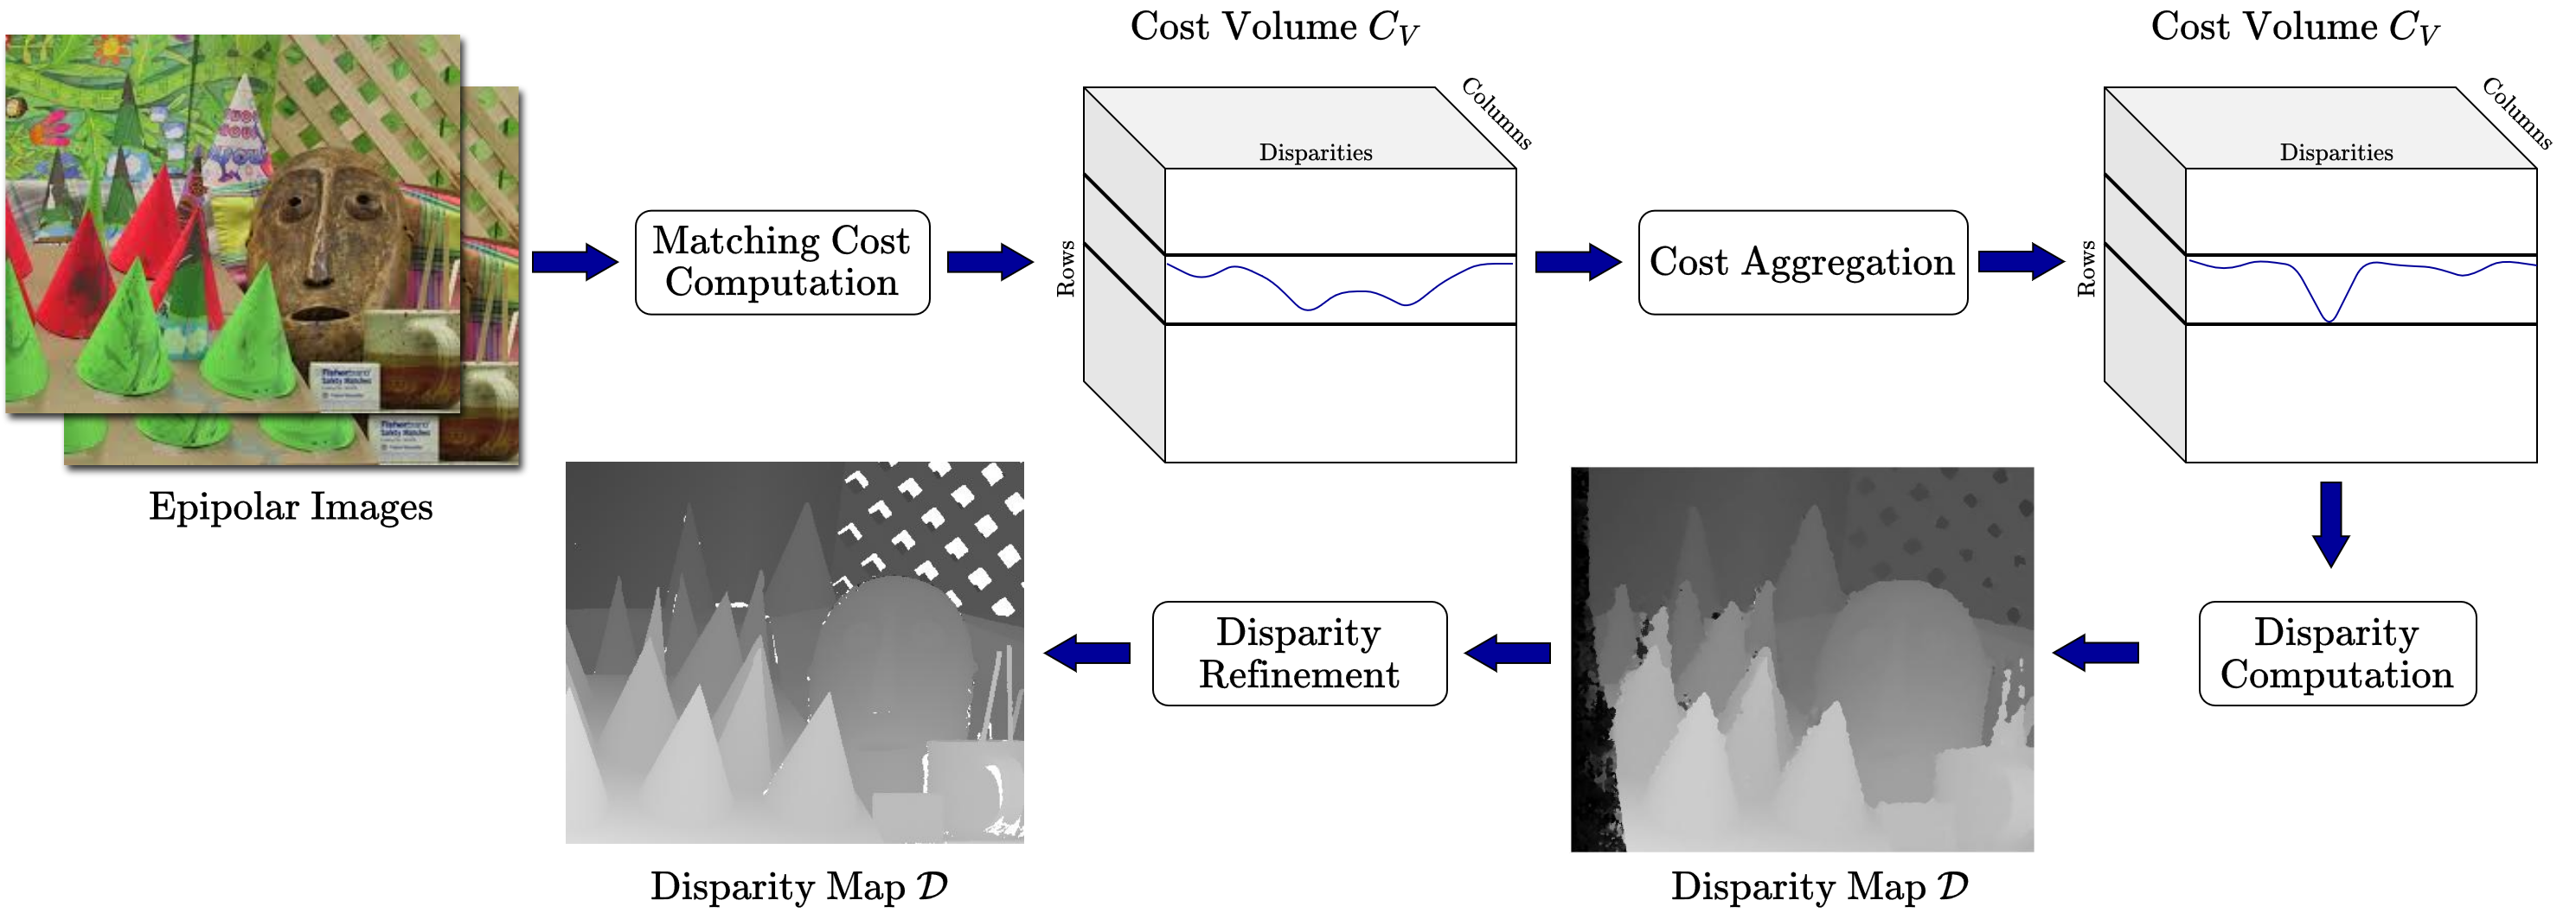
\includegraphics[width=\linewidth]{Images/Chap_1/stereo-matching_pipeline.png}
	\caption{The different steps of classical dense stereo-matching algorithms.}
	\label{fig:stereo_matching_pipeline}
\end{figure}

\subsubsection{Cost Volume Computation}\label{sec:cost_volume_computation}
The cost volume computation can be described as follows: given a range of considered disparity, the cost of matching every pixel of the reference image to every pixel in of the secondary image in the disparity range is stored in an array of data called cost volume (\Cref{fig:cost_volume})\commanue{Avant de dire que c'est stocké dans un cost volume, je dirais que le coût représente la similarité entre deux pixels des deux images. Dans cette première phrase tu mentionnes beaucoup le terme de coût }. The matching cost is evaluated using a cost function, which is a mapping $f$ from subsets of the left and right images to $\mathbb{R}$\commanue{Tu peux peut-être rajouter que la focntion de coût est là pour donner un score sur la similarité entre les pixels de deux images avant de te lancer dans les exemples}. Example\commanue{C'est bizarre le terme example} \ref{ex:cost_functions} provides different examples of cost functions\commanue{Peut-être ajouter une définition générique de la fonction de coût avant de parler des exemples}.

\begin{example}\label{ex:cost_functions}
	Simple examples of cost functions include the Sum of Absolute Differences (SAD), the Zero Normalized Crossed Correlation (ZNCC)  \cite{hannah_computer_1994}, the CENSUS transform \cite{zabih_non-parametric_1994} and MC-CNN \cite{zbontar_stereo_2016}.
	
	Given two windows $W_L$ and $W_R$ from the left and right images, the SAD cost function is defined as follows:
	\begin{equation}
		f_{SAD}(W_L, W_R)  = \sum_i\sum_j | W_L(i,j) - W_R(i,j) |
	\end{equation}
	Low $f_{SAD}$ values indicate that the windows are similar, while high values indicate noticeable differences. A $f_{SAD}$ value of $0$ indicates that the windows are identical. This cost function is probably the simplest cost function one could imagine, and will be used to detail\commanue{le to detail est en trop à mon sens car tu as déjà une autre verbe après} in \Cref{chap:propagating}\comloic{juste used in chapter 4 to didactically} to didactically illustrate how uncertainty models can be propagated throughout a cost function. However, this cost function is not usually used\comloic{usually used? ;-) en gro c'est pas robuste à un bias radio entre les images ni un offset, or meme dans les conditions CO3D (et déjà c'est synchrone ou quasi et pas commun), tu as des objets imagé a la meme heure mais selon l'angl de prise de vue la radio peut différer donc SAD dans les chous}\commanue{in practice ?} in stereo matching algorithms as more efficient cost functions have been proposed since\commanue{tu pourrais juste préciser que ce n'est pas efficace car juste baser sur des différences radio}. It can be a fast and easy way to have a first estimate of similarities between multiple patches. The SAD can also be used for motion estimation and image/video compression \cite{richardson_h264_2006}.
	
	The ZNCC cost function is defined as the correlation coefficient between both images:
	\begin{equation}
		f_{ZNCC}(W_L, W_R)  = \sum_i\sum_j \frac{(W_L(i,j)  - \tilde{W}_L) (W_R(i,j)  - \tilde{W}_R) }{\sigma_L\sigma_R}
	\end{equation}
	where $\tilde{W}$ refers to the mean value of a window, and $\sigma$ its standard deviation. Negatively correlated windows would present a ZNCC value of $-1$ and positively correlated windows present a ZNCC value of $1$. Contrary to the SAD cost function, matching windows will be indicated by a high value of the ZNCC. It is thus not \textit{strictly} a cost function but rather a similarity function. It is not a problem, as multiplying $f_{ZNCC}$ by $-1$ will transform it into a cost function. Another formulation could be to say that the $ZNCC$ is a \textit{maxitive} cost function, in the sense where potential matches are found by searching for its maximum. Conversely, the SAD is a \textit{minitive} cost function in the sense where potential matches are indicated by a minimal cost.\commanue{Avantages? Inconvénients? Est-ce qu'on l'utilise? Non, ça présente pas mal d'intérêt notamment dans les zones homogènes mais pour CO3D on vise des trucs sympas en urbain vu que bon, l'argent il est là... donc il faut pas trop baver enfin adhérer, donc on préfère census}
	
	The CENSUS cost function\comloic{à l'oringe c'est un filtre, Census Filter, ça devient dans le langage commun une cost function juste parce que si tu l'applique à deux images et que tu ajoutes la distance de hamming bein ça marche bien} needs a bit more detailing\commanue{mon anglais pourri penche pour needs to be a little more detailed}\comloic{+1}. For a squared window $W$ with a side of $2n+1$ pixels, we first compare the value of each pixel of the window with the center pixel. This gives a binary string where $1$ indicates that the value of the pixel is superior to that of the center pixel. For instance if we consider the two $3\times3$ following windows $W_L, W_R$:
	$$
    \begin{bmatrix}
        155 & 133 & 97 \\
        80 & 110 & 132 \\
        100 & 102 & 120
    \end{bmatrix}
    \qquad
    \begin{bmatrix}
        175 & 153 & 133 \\
        100 & 130 & 152 \\
        120 & 135 & 125
    \end{bmatrix}
	$$
	Then comparing each of their pixel to the center of the windows will yield the following binary strings (expressed here as matrices):
	$$
    \begin{bmatrix}
        1 & 1 & 0 \\
        0 &  & 1 \\
        0 & 0 & 1
    \end{bmatrix}
    \qquad
    \begin{bmatrix}
        1 & 1 & 1 \\
        0 &  & 1 \\
        0 & 1 & 0
    \end{bmatrix}
	$$
	The cost function $f_{CENSUS}$ is finally obtained by taking the Hamming distance (\ie the number of different bits between those two strings:
	\begin{equation*}
		f_{CENSUS}(W_L, W_R) = 3
	\end{equation*}
	
	The CENSUS cost function compares relative intensity variations, it is thus less sensitive to variations of intensities between images, such as a change of exposure for instance. Similarly to the SAD, two similar patches will tend to have a low value.
	
	The MC-CNN cost function \cite{zbontar_stereo_2016} is using a convolutional neural network architecture to measure the similarity between patches\commanue{ça mérite un peu de schémas}\comloic{la partie convolutionnelle elle permet de décrire un patch, un peu comme un descripteur sift quoi, après il y a une mesure de similarity (cosine similarity) branchée derrière et une loss qui force la sortie du nn à tendre vers des patchs utiles pour le matching en particulier}. It was train on $11\times 11$ patches from stereo images from the Kitti \cite{geiger_vision_2013, menze_object_2015} and Middlebury \cite{scharstein_taxonomy_2001,scharstein_high-accuracy_2003,hirschmuller_evaluation_2007,scharstein_learning_2007,scharstein_high-resolution_2014} datasets. They first trained their network to compute a vector of features for each patch\commanue{Modèle siamois même réseau pour extraire les features entre les iamges}. They then trained a second network to compute the similarity measure between both feature vectors. They also proposed a so-called ``fast'' architecture, which directly computes the cosinus between both vectors, thus by-passing the need of a second network for similarity\commanue{Avec le cosinus simple produit scalaire donc}\comloic{ok tu précises des choses ici, mais du coup plus haut, au moment ou tu dis MCCNN c'est un CNN pour mesurer la similarité c'est pas trop ça... enfin faut choisir, MCCNN c'est soit un outil, celui du papier, soit un réseau de neurones mais qui ne sort pas une mesure de similarité il sort juste un descripteur à la sift}. As ZNCC, MC-CNN is a similarity measure\comloic{ok donc soit c'est une mesure de similarité, mais alors là c'est pas juste un convolutional neural network, c'est soit l'enchainement de deux cnn soit un cnn et une vraie mesure de similarité qui n'a pas besoin de MCCNN pour être une mesure de similarité d'ailleurs}, but can easily be converted into a cost function. Although it has been trained on stereo images of autonomous cars (Kitti) and stereo images of toys (Middlebury), it generalizes well to our satellite images\commanue{cite la publi de Véro et Loïc}.
\end{example}
	
Using the chosen cost function $f$, a cost volume $C_V$ is then evaluated by measuring the cost of matching every patch in the left image to every pixel in the right image in the given disparity range\commanue{ça ressemble bcp à l'intro, donc je pense que ton intro devrait démarrer par la fonction coût et ensuite tu embrailles comme tu le fais avec le cost volume}. The cost volume as thus three dimensions, namely rows, columns and disparity:
\begin{equation}\label{eq:cost_volume}
    C_V(row, ~col, ~d) = f(W_L(row, ~col),  W_R(row, ~col+d))
\end{equation}
where $W_L(row, ~col)$ is a window centered on the pixel at coordinates $(row, ~col)$ in the left image, and $W_R(row, ~col+d)$ is a window centered on the pixel at $(row, ~col+d)$ in the right image. We usually add some padding to the images to avoid problems near borders where the column $col+d$ would not be defined. Given a pixel in the left image $(row, ~col)$, matching cost values for every considered disparity form what is called a cost curvecurve. In theory, the correct disparity for a match is determined by finding the minimum of the cost curve (for minitive cost functions such as SAD or CENSUS). In the rest of this thesis, we will consider that a cost function is always minitive unless specified otherwise. In practice, directly determining correct disparities from the cost volume is not efficient as geometric structure of the scene is not yet taken into account\commanue{Je ne suis pas sure de comprendre. Tu veux parler du fait que sans optimisation on a pas de bons résultats ? C'est pas évident de voir ce que tu sosu-entends par prendre en compte la géométrie de la structure étant donné que c'ets justement ce qu'on cherche a estimé. Peut-être dire juste préciser le meilleur candidat donc approche locale sans tenir compte du voisinage des disparités ne donne pas des choses terribles et donc un exemple pour montrer que c'est très bruité.}. \Cref{fig:cost_volume} represents a cost volume, and one of its cost curves where potential matches have been highlighted\commanue{peut-être mettre cette phrase avant quand tu définis les termes. Ensuite tu pars sur des remarques pour revenir sur un schéma}. 

\begin{figure}
	\centering
	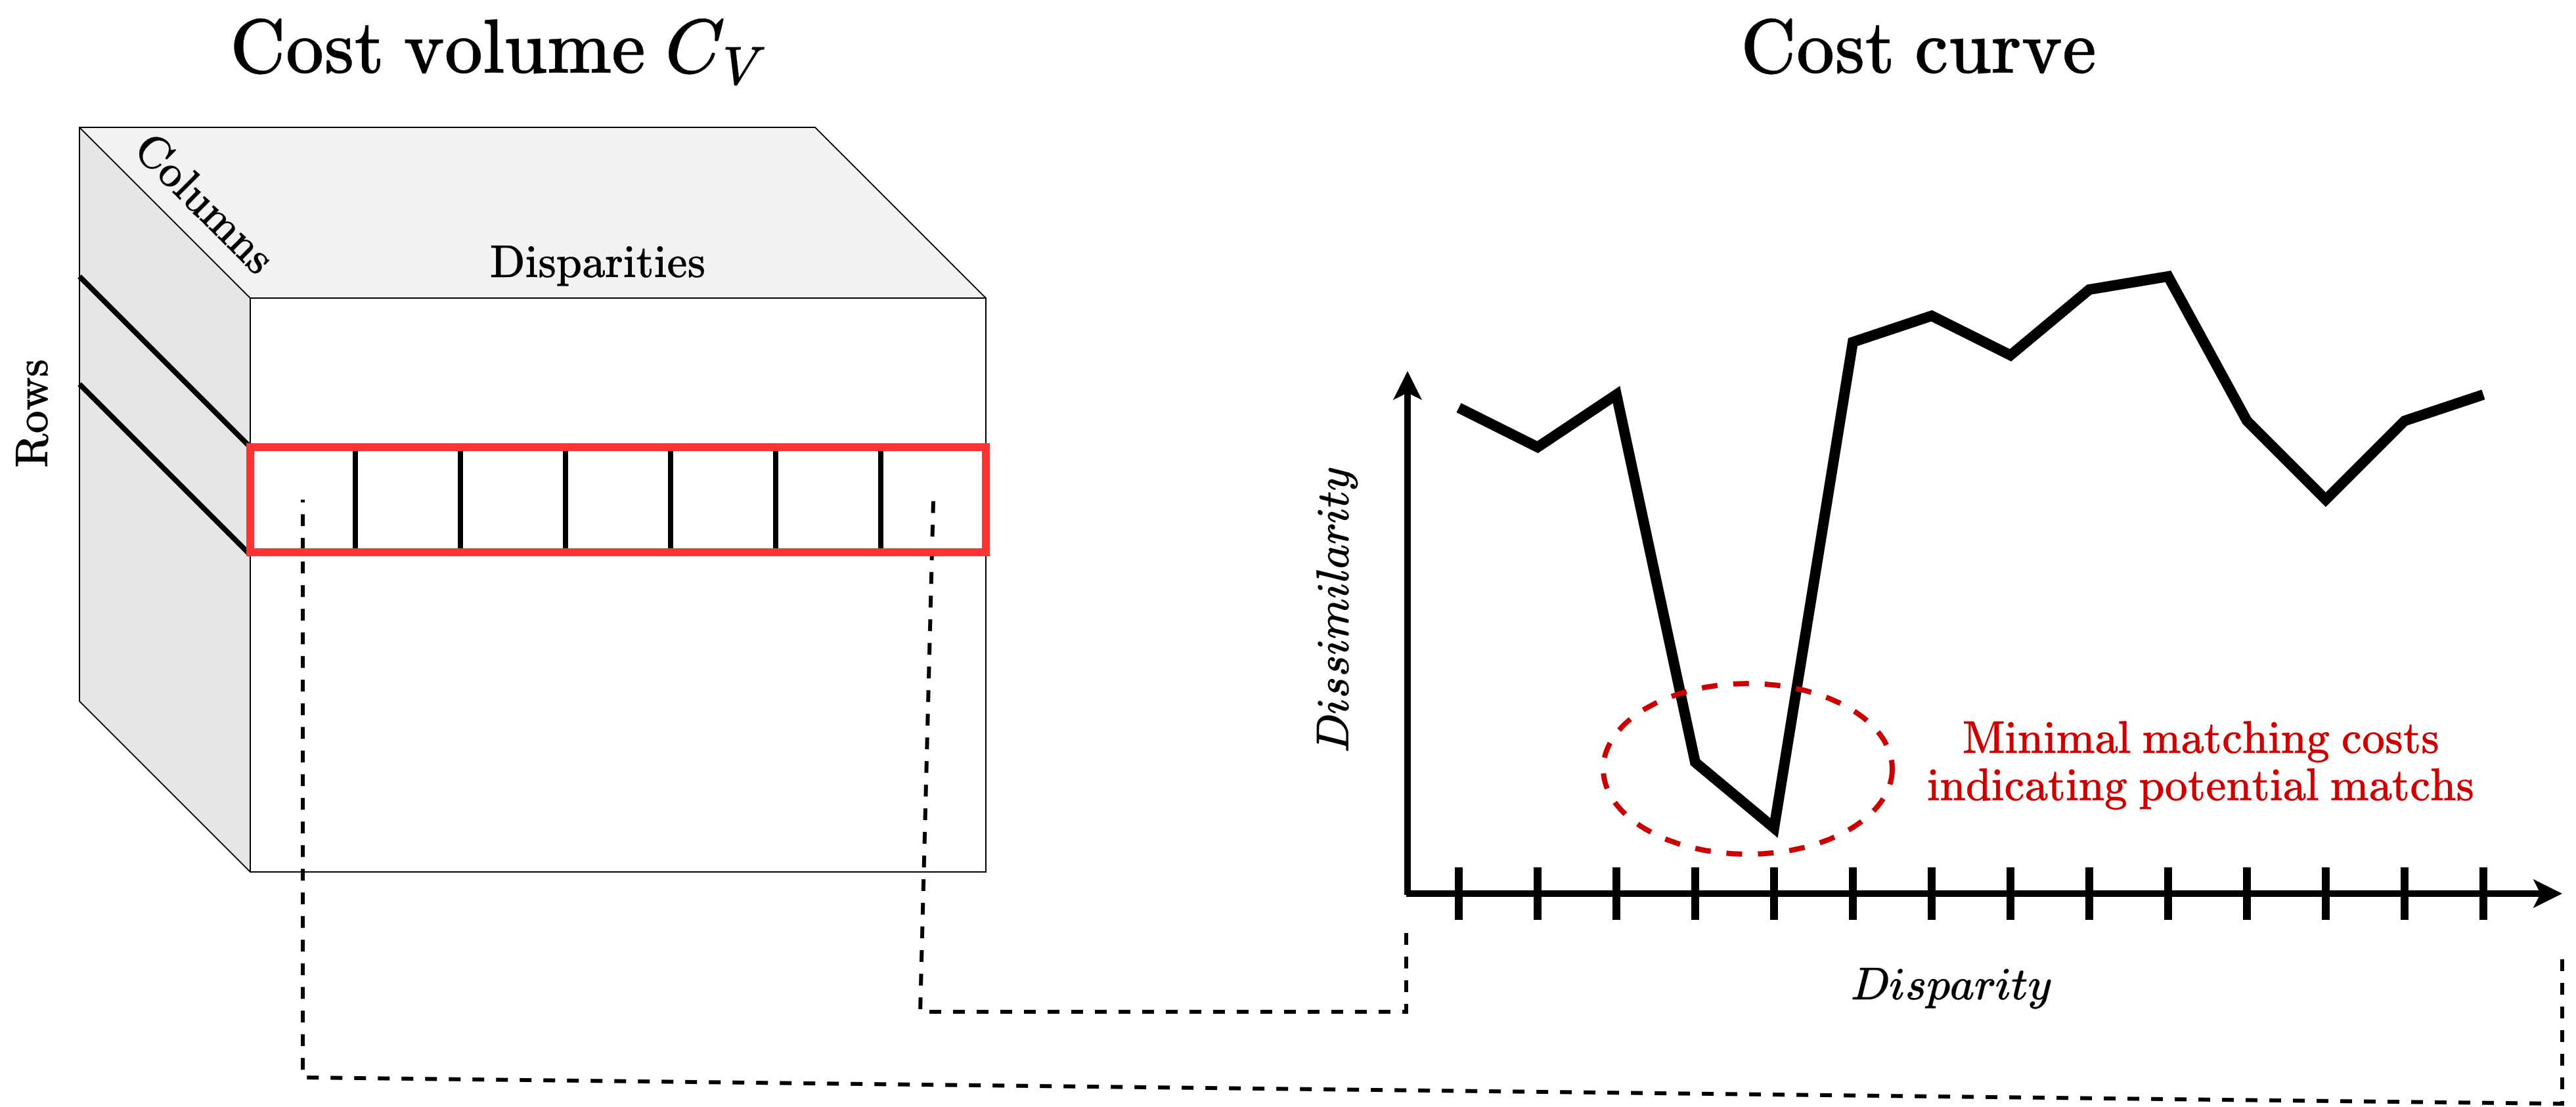
\includegraphics[width=\linewidth]{Images/Chap_1/Cost_volume.png}
	\caption{Matching cost volume and one of its cost curve}
	\label{fig:cost_volume}
\end{figure}\commanu{dans le texte de la figure: minimal matching cost indicating potential match, sans pluriel. ou sinon matchs-> matches}

The usage of windows\commanue{in the calculation of the cost function} allows to take into consideration the surrounding of pixels to better measure their similarity. However, window based approaches\commanue{ajouter peut-être: , mostly square-shaped,} also present the disadvantage of struggling to correctly identify matches near object borders \cite{hirschmuller_real-time_2002}. This is usually called an adherence effect, represented in \Cref{fig:adherence_window}\commanue{Pour montrer l'adhérence il te faut aussi un schéma en 3D pour que les gens comprennent bien ce que voit l'image de gauche et celle de droite. Après tu peux rester 1D pour que ce soit plus simple. Il te faut aussi (oui c'est relou l'adhérence) le résultat en terme de disparité pour montrer pourquoi on appelle cela adhérence}. In this figure, there are three objects represented with three different colors. Centered pixels of both windows do not match, contrary to the rest of the windows which are exactly the same. Sliding the right window in both directions would lead to higher matching costs, as the windows would be even more dissimilar\commanue{je ne suis pas sure de comprendre la phrase. L'adhérence c'est justement que tu vas te retrouver à trouver qu'à cause du voisinage tu vas pas associer le bon pixel. En général tu descends du building un peu plus tard que dans la réalité. En fait ce qu'il te manque dans ta figure c'est qu'est-ce qu'il faudrait associer comme bonne disparité et qu'est-ce que tu as associé en fait du fait de la fenêtre utilisée.}. This illustrates the fact that matching windows do not necessarily mean that the center pixels constitute a match. Other work have been proposing to use a spatial weighting \cite{kuk-jin_yoon_locally_2005}, segmentation \cite{hutchison_segmentation-based_2007}, windows with different shapes \cite{ke_zhang_cross-based_2009, buades_reliable_2015} to solve this problem. 
\begin{figure}
	\centering
	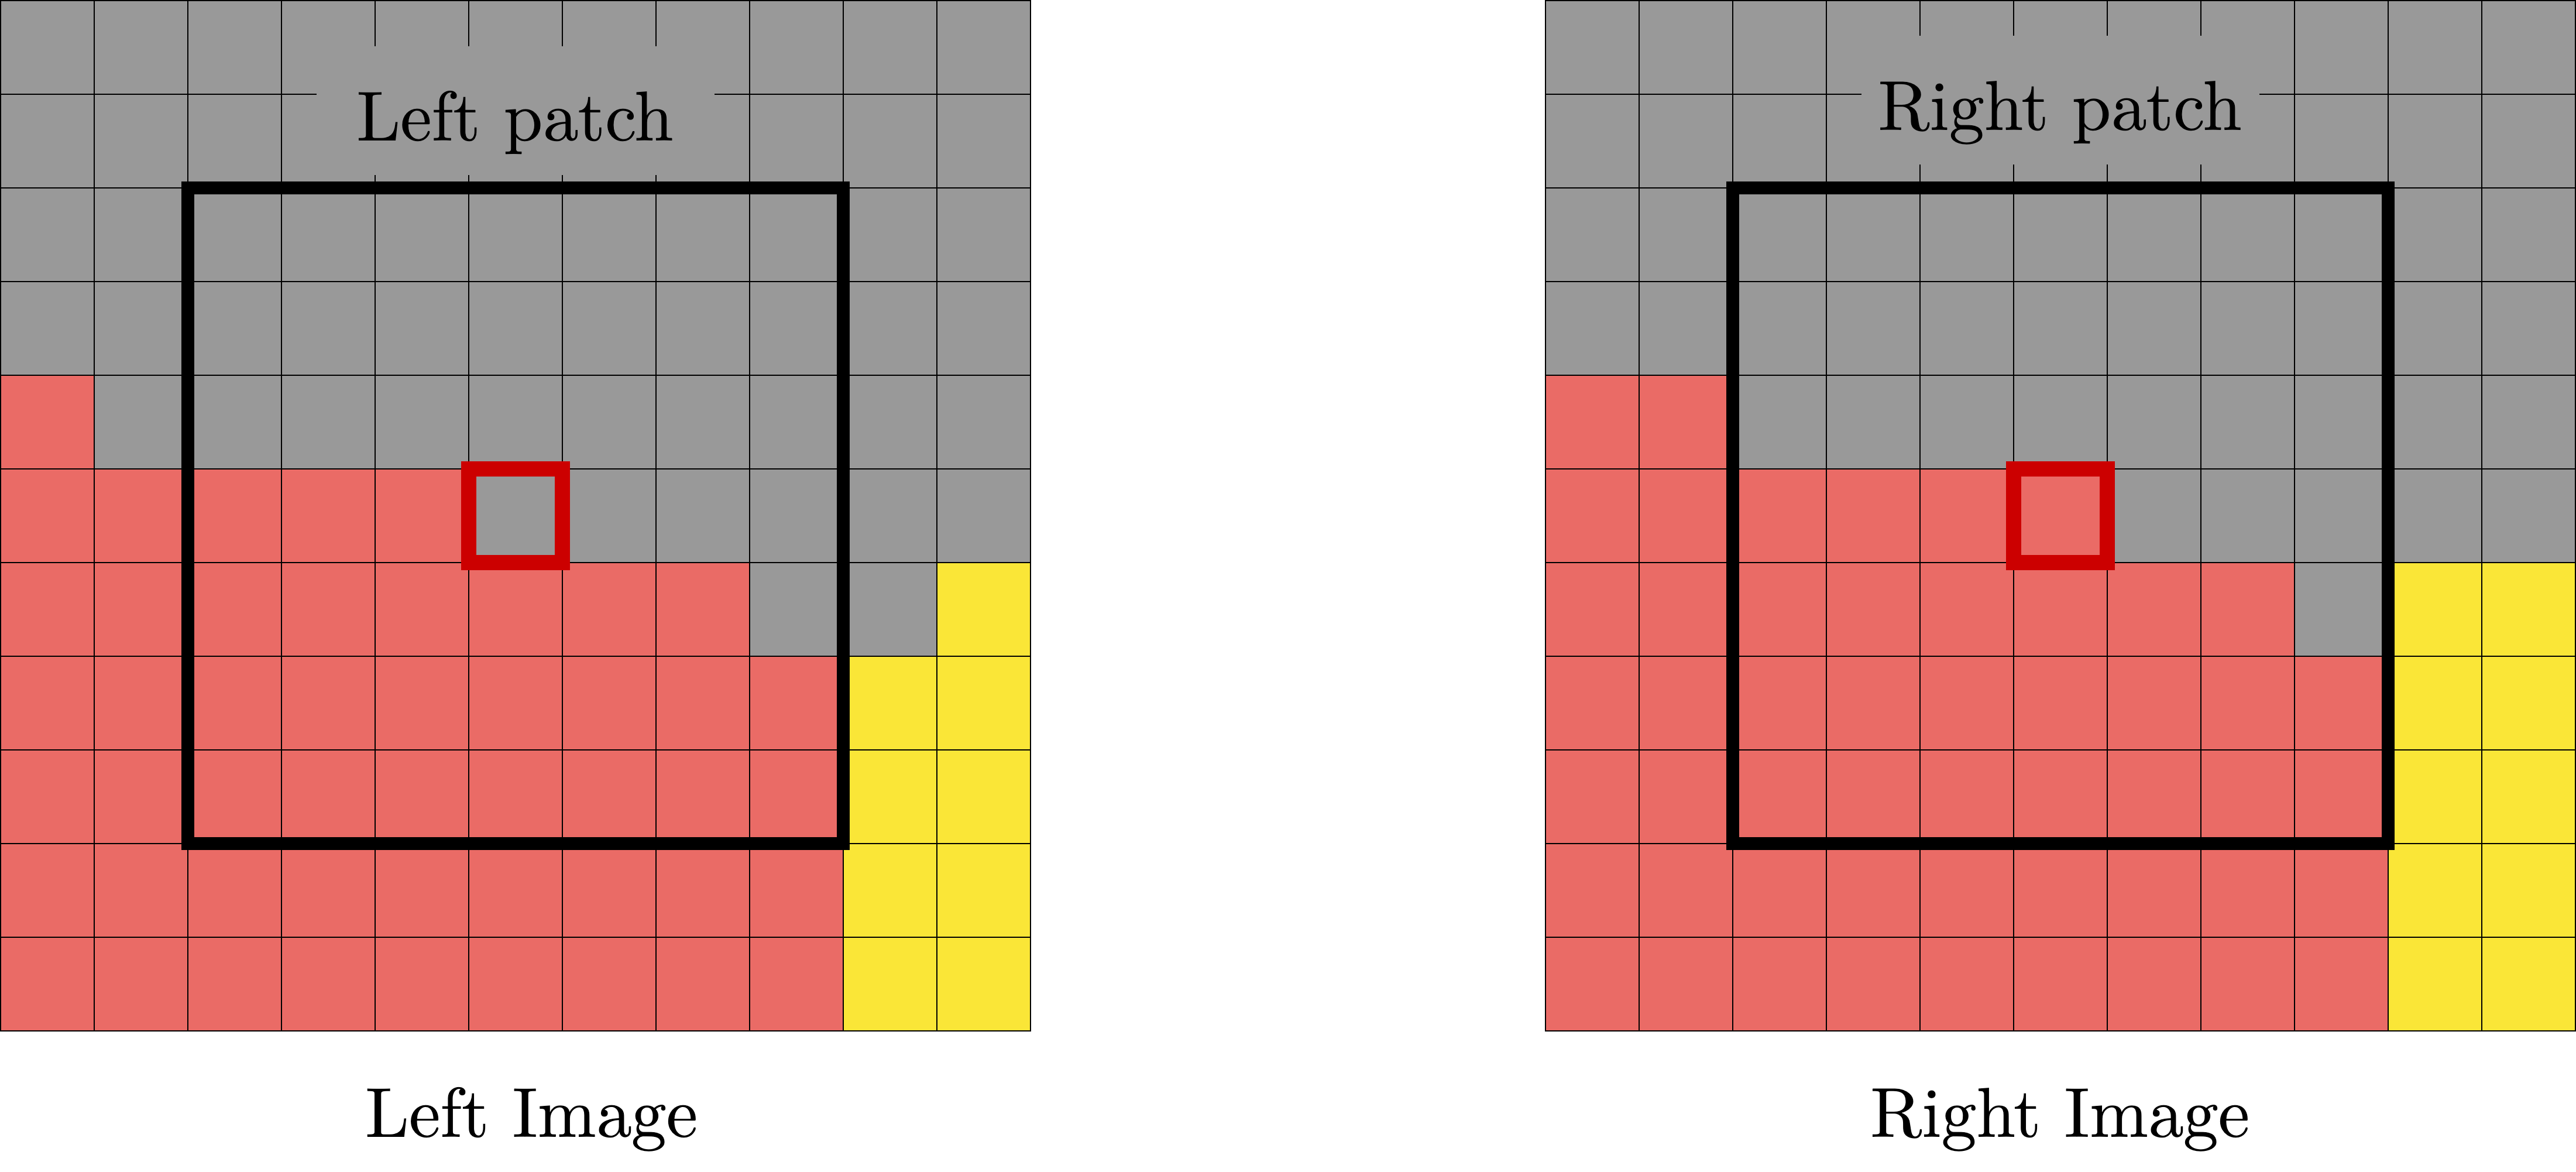
\includegraphics[width=\linewidth]{Images/Chap_1/Adherence_window.png}
	\caption{Adherence problem when comparing two patches between epipolar images}
	\label{fig:adherence_window}
\end{figure}

After computing the matching cost, information regarding the geometric structure of the scene\commanue{c'est pas ton meilleur choix de terme} can be incorporated in the cost volume. A first approach is to aggregate different parts of the cost volume. Usually, costs of pixels belonging to the same objects are aggregated using different methods for segmentation \cite{ke_zhang_cross-based_2009, ji_superpixel_2021}. This part is not always present in algorithms, as we will see next there exists regularization algorithms designed with the same purpose. 

\subsubsection{Semi Global Matching and Disparity Computation}
\commanu{comme dit au début de la partie dense matching, pas évident de retrouver l'ordre de présentation du début. etre cohérent avec le déroulé du début du dense matching, sinon pas évident de suivre pour un lecteur}
Computing the disparity map from the cost volume can be done in several ways. So-called local methods apply a direct \textit{winner-takes-all} strategy, where the $\argmin$ of every cost curve is kept as the selected disparity. This has the disadvantage on allowing multiple pixels from the right image to be matched to the same pixel of the left image\comloic{je vois pas trop pourquoi ça ne peut être le cas pour une méthode globale ? je rate un truc ?}. On the other hand, global method use the information contained in the cost volume to solve an optimization problem, where the objective is to compute the disparity map $\mathcal{D}$ minimizing an energy function expressed as follows:
\begin{equation}
    E(\mathcal{D}) = E_{data}(\mathcal{D}) + \lambda E_{smooth}(\mathcal{D})
\end{equation}
where $\lambda$ is a scalar for tuning the importance of the regularization term $E_{smooth}$. Usually, the data term is directly computed from the cost volume as:
\begin{equation}\label{eq:global_methods}
    E_{data}(D) = \sum_{row,~col}C_V(row, ~col,~D(row, ~col))\commanue{C'est pas le même symbole D que dans la précédente équation}
\end{equation}
The regularization term $E_{smooth}$ can take numerous forms, usually measuring if the neighbouring disparities possess similar values \cite{scharstein_taxonomy_2001}. Then a local minimum for this energy is found using various methods, such as Markov Random Fields \cite{boykov_markov_1998, sun_stereo_2003}, graph cuts \cite{kolmogorov_computing_2001} or minimum spanning trees \cite{zureiki_stereo_2008, qingxiong_yang_non-local_2012}. Those algorithms improves performances in comparison to local methods, but can be computationally expensive.

The most popular method is actually Semi-Global Matching (SGM) \cite{hirschmuller_accurate_2005}: it aims at incorporating regularization constraints to the cost volume similarly to global methods, in order to be processed\commanue{j'aurais tendance à mettre while being processed with relative low computational cost pour montrer que SGM cherche à avoir les avantages des deux côtés}\comloic{ouais parce que il y a aussi un cost volume dans de vraies méthode globale genre basées sur les graphes et résolue par komlogorov ou son copain donc là c'est surtout que c'est semi global parce qu'on résoud pas le problème initial on fait une modélisation simplifiée en réduisant tout ça a quelques chemins} like local methods. It is, in a way, in-between local and global methods. This is the method we will\commanu{j'aurais enlevé le will} use in the CARS pipeline for experiments in this thesis. In short, for each pixel, the SGM algorithm looks into neighbouring pixels recursively, and increases the cost of disparities that do not present a consensus\comloic{pas sur de te comprendre?} amongst neighbours \comloic{je pense que si tu veux être rigoureux tu dois présenter le CV comme un graphe, avec les noeuds qui sont le terme Edata c'est à dire les couts de similarité et les liens qui sont le termes Esmooth. Ensuite SGM dit simplement "je vais pas résoudre le problème dans sa globalité je vais le réduire à une dimension et répéter 4/8 fois ce job pour 4/8 directions}. Although the formulation of the SGM algorithm can be expressed in a few equations, understanding how its inner workings is more complex. We will first present its mathematical formulation in \cref{eq:sgm,eq:sgm_penalties}, and use \Cref{fig:sgm} to illustrate its effect on (a portion of) a cost curve. Formally, for every pixel $p=(row, ~col)$, the cost volume is explored in multiple directions as in \Cref{fig:sgm_directions}.

\begin{figure}
	\centering
	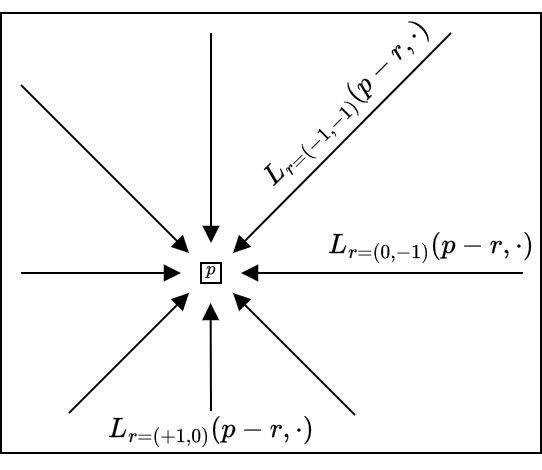
\includegraphics[width=0.5\linewidth]{Images/Chap_1/SGM_directions.png}
	\caption{SGM regularization with $8$ directions}
	\label{fig:sgm_directions}
\end{figure}

The cost is regularized for each direction $r$ to take into account the best disparity $d$ along that direction. A direction can be for instance $r=(0,~1)$, meaning that we will look at same row and travel to the right of the image when browsing direction $r$. Given two positive scalars $P_1<P_2$, the regularized cost $L_r$ along direction $r$ and at disparity $d$ is expressed with the following recursive formulation:
\begin{align}\label{eq:sgm}
    L_r(p,d) = C_V(p,d) + \min_\delta \left(L_r(p-r,~\delta) + R(d, ~\delta)\right)\commanue{elle est bizarre la formulation de SGM. Je comprends le $\delta$, c'est pas évident de retrouver la formule de l'article}
\end{align}
where $R(d, ~\delta)$ equals:
\begin{align}
    R(d, ~\delta) = &P_1\cdot\mathds{1}(|d-\delta|=1) + P_2\cdot\mathds{1}(|d-\delta|\geqslant 2) - \min_k L_r(p-r,~k) \label{eq:sgm_penalties}
\end{align}
Here, $\mathds{1}$ is the indicator function. The first term of \cref{eq:sgm} is the cost volume, which can be compared to $E_{data}$ in \cref{eq:global_methods}. The second term is similar to the regularisation term $E_{smooth}$. This term can be seen as the regularized cost $L_r(p-r, ~d)$ from the previous pixel in direction $r$, but shifted of $P_1$ for neighbouring disparities $d\pm1$, and of $P_2$ for further disparities. The term $\min_k(L_r(p-r,~k))$ prevents $L_r(p,\cdot)$ to diverge to very high values by ensuring that the minimum of $L_r(p-r,~\delta) - \min_k(L_r(p-r,~k))$ always equals $0$. \Cref{fig:sgm}\commanue{J'avoue que j'ai du relire le paragraphe plusieurs fois, j'ai un peu  de mal avec ta notation qui se veut très générique. C'est un peu le même prinicipe pour la figure. C'est ton choix donc à voir si ça parle plus aux autres.}\commanu{en effet pas évident. peut etre un exemple plus concret sur ce que ca permet de faire et donc de mieux comprendre la motiv de l'algo et donc l'algo in fine. mais pas évident de toute façon de bien l'expliquer} presents $L_r(p-r,~\delta) + R(d, ~\delta)$ for two different disparities $d$ and $d+1$ in the blue frame. The minimum of each curve $L_r(p-r,~\delta) + R(d, ~\delta)$ (blue arrows in the figure) are then added to the matching cost $C_V(p,d)$ to obtain the final regularized cost $L_r(p,d)$. Note that in \Cref{fig:sgm}, the minimum of $L_r(p-r,~\delta)+R(d+1, ~\delta)$ equals $0$, thus $C_V$ is unchanged for this disparity. This is because $d+1$ is the minimum of $L_r(p-r,~\cdot)$. In a way, the regularized matching cost will be a mixture between $C_V(p,\cdot)$ and $L_r(p-r,~\cdot)$. Indeed, the regularized cost $L_r(p-r,\cdot)$ indicates that disparity $d+1$ seems likely, while disparity $d$ is unlikely. On the other hand, the matching cost $C_V(p,\cdot)$ indicates that both disparities $d$ and $d+1$ are likely. The final regularized cost $L_r(p-r,\cdot)$ takes into account that both $C_V(p,\cdot)$ and $L_r(p-r,\cdot)$ agree that $d+1$ is likely, but that there is a disagreement on $d$, and thus slightly increases the regularized cost $L_r(p,d)$. Disparities that seem unlikely to both $C_V(p,\cdot)$ and $L_r(p-r,\cdot)$ lead to a larger increase of the regularized cost $L_r(p,\cdot)$ \commanu{mieux sur la fin, ca pourrait donc etre illustré avec un cas plus concret. Ta figure de l'enfer explique l'algo mais on a a du mal à "voir" ce que ca fait, comme tu l'expliques plutot bien sur cette fin de paragraphe. Donc comme dit, un petit exemple plus concret aiderait}.
\begin{remark}
    For the sake of the remark, let suppose that $P_1=P_2$ for now. The value added to $C_V(p, ~d)$ in \eqref{eq:sgm} will be lower than $P_2$ only if $(L_r(p-r,~d) - \min_k L_r(p-r,~k)$ is less than $P_2$. This means that we will always add a penalty of $P_2$ to the cost $C_V$, except if $L_r(p-r,~d)$ is less than $P_2$ away from its minimum. $P_2$ thus represents the penalty that must be overcame in $L_r(p-r,~d)$ in order to not penalize $C_V(p,d)$, or slightly penalize $C_V(p,d)$.
    
    If $P_1<P_2$, then we can draw similar conclusions, except that we also accept to reduce the penalty to $C_V(p,d)$ if a neighboring disparity, \ie $d\pm1$ is less than $P_1$ away from the minimum. Hopefully this remark, equations and figures helped in making sense of the SGM algorithm\commanu{bizarre ta dernière phrase, pas très anglais, j'enleverais. Par contre, intéressant de donner des cas d'exemples P1=P2, P1 très petit par rapport à P2, et tu pourrais illustrer l'impact sur une petite image bien choisie... suivant le temps bien sur, tu vois}
\end{remark}

Formulation of \cref{eq:sgm} is recursive, and thus must be initialized. The regularization curves thus begin at the borders of the image and their value is, by convention, $0$ when undefined. For instance with $r=(0,1)$:
\begin{align*}
    L_r((row, 0),d) = C_V(row, 0 ,d)
\end{align*} 

\begin{figure}
	\centering
	\includegraphics[width=\linewidth]{Images/Chap_1/SGM.png}
	\caption{Schematic explanation of the SGM algorithm in a single direction $r$. Top: regularized cost $L_r$ at $p-r$. In the blue frame $L_r(p-r,~\delta)+R(d,~\delta)$ for two consecutive disparities $d$ and $d+1$ ($L_r-\min_k L_r$ appears in dotted line for clarity). Penalty $P_1$ appears in yellow, penalty $P_2$ appears in red, the minimum of each curve is denoted by a blue arrow. Bottom left: cost volume $C_V$ at $p$. Bottom right: regularized cost $L_r$ at $p$ where the minima of all $L_r(p-r,~\delta)+R(d,~\delta)$ have been added.}
	\label{fig:sgm}
\end{figure}\comroman{C'est un peu le schéma de l'enfer, mais c'est ce que j'ai trouvé de mieux pour expliquer SGM.}\commanue{comme je le dis plus haut, j'avais que le côté très générique des notations n'ai pas facile. Après il y a des trucs intéressants et de tout façon c'est pas simple à schématiser.}\comloic{est ce que si tu le fais que pour une disparité c'est pas plus simple à présenter ? dans le dernier morceau en rose en bas à droite, j'ai eu du mal à comprendre l'extrapolation de la courbe pour les disparités du point r-1 dont tu ne présentes pas les courbes, ça m'a un peu perturbé. Ou alors tu ne mets à jour que les coeffs des deux disparités étudiées peut être ? Après ce que tu montres c'est la conséquence de l'implémentation mais je sais pas si on capte la motivation. Peut être qu'avec des objets genre bati et sol ou quoi ce serait plus palpable mais enfin c'est pas simple je le reconnais}

When all regularized cost curves $L_r$ have been computed, they are summed to obtained the regularized cost volume $C_V^{SGM}$:
\begin{equation}
    C_V^{SGM}(p, d) = \sum_r L_r(p,d)
\end{equation}
The cost volume $C^{SGM}_V$ contains the regularized cost for\commanue{alors il manque la fin de la phrase} 
Since the original paper \cite{hirschmuller_accurate_2005}, different variations of the SGM algorithm have been proposed. For instance using different regularization paths \cite{facciolo_mgm_2015} or a different strategy for the aggregation of costs \cite{poggi_learning_2016}.

The main problem of SGM regularization is its reluctancy to detect discontinuities in the disparity map. Indeed, SGM penalizes disparity changes, therefore strong variations of disparity are badly reconstructed\comloic{je dirais que ça dépend qd meme fortement de ton termes Esmooth... si P2 et P1 sont tout piti piti piti bah pas de pb sur les bati mais par contre ça reste bien bruité dans les zones homogènes}. For instance near the border of a building, instead of a having the desired discontinuity in the disparity map, there can be a smooth transition \comloic{c'est dommage de pas parler du termes Esmooth ici, tu y es presque avec "smooth". C'est typiquement que SGM n'applique pas le saut de discontinuité tant que Esmooth reste prépondérant devant Edata, le fait que la transition soit progressive c'est plutôt lié à la somme des 8 directions puisqu'elles sont sommées avec le même poids indépendant de la pertinence de ce choix (chemin visible continue entre r-1 et r)} between the roof and the road, leading to rounded borders and soft edges of buildings. This is even reinforced with the window adherence problem presented in \ref{fig:adherence_window}. \Cref{fig:DSM_toulouse} presents a comparison of two DSM: one obtained directly from LiDAR HD data \cite{monnet_lidarhd_2023}, and the other using the CARS pipeline with the CENSUS cost function over a $5\times5$ window and with SGM regularization. We can see on this figure that the border of the buildings obtained using SGM regularization are not as sharp and precise as those of the LiDAR DSM \comloic{alors.. bon... après t'as qd meme une histoire de résolution aussi}. To provide a solution to this problem, one might limit the SGM regularization to pixels from the same object, defined\commanu{bizarre le defined using, je ferais plus direct from the same object using a segmentation} using a segmentation \cite{dumas_improving_2022}. This method relies on the quality of the segmentation method used and can become quite costly. It has not been considered in the context of this thesis. \todoroman{est-ce que c'est prévu de l'utiliser dans le pipeline CO3D? Sinon je peux aussi dire que je ne considère que ce pipeline là}\commanu{à priori oui via 3SGM qui contraint SGM et les segmentation de yannick dans SLURP, c'est en test cette année}

\begin{figure}
    \centering
    \begin{subfigure}[t]{0.5\linewidth}
        \centering
        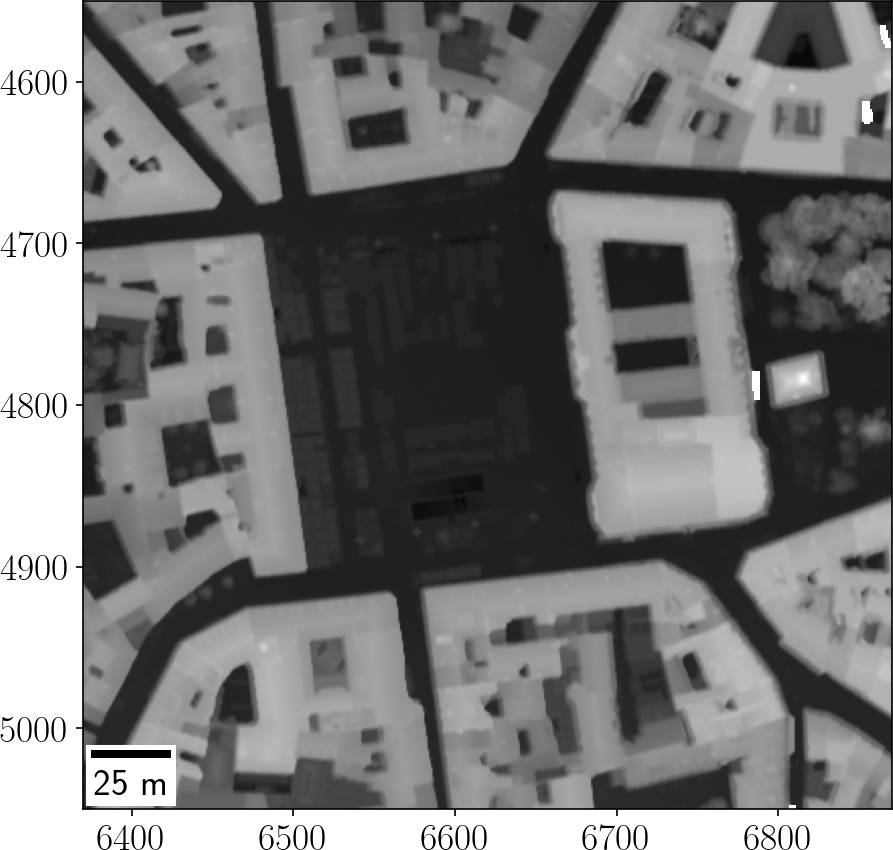
\includegraphics[height=6cm]{Images/Chap_1/DSM_Capitole_LiDAR.png}
        \caption{DSM from LiDAR HD data,\\Place du Capitole}
        \label{fig:DSM_capitole_lidar}
        %\begin{minipage}{.12cm}  % Multiline captions misalign figures
        %    \vfill              % This blank minipage is used to align
        %\end{minipage}          % images
    \end{subfigure}\hfill
    \begin{subfigure}[t]{0.5\linewidth}
        \centering
        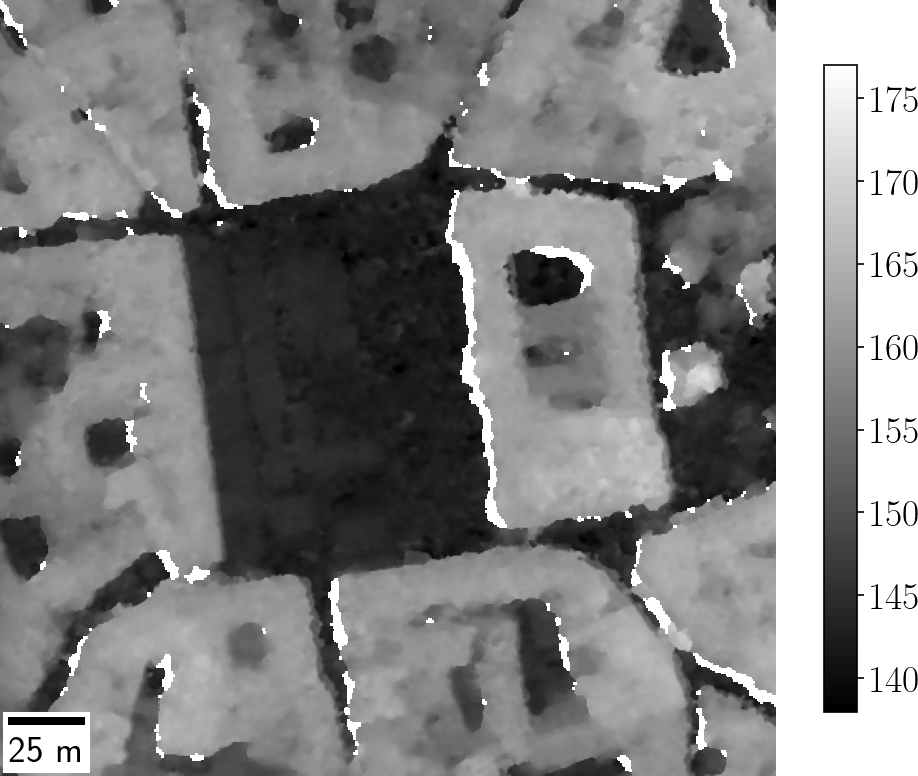
\includegraphics[height=6cm]{Images/Chap_1/DSM_Capitole_CARS.png}
        \caption{CARS DSM from Pléiades images,\\Place du Capitole}
        \label{fig:DSM_capitole_cars}
    \end{subfigure}
    \begin{subfigure}[t]{0.5\linewidth}
        \centering
        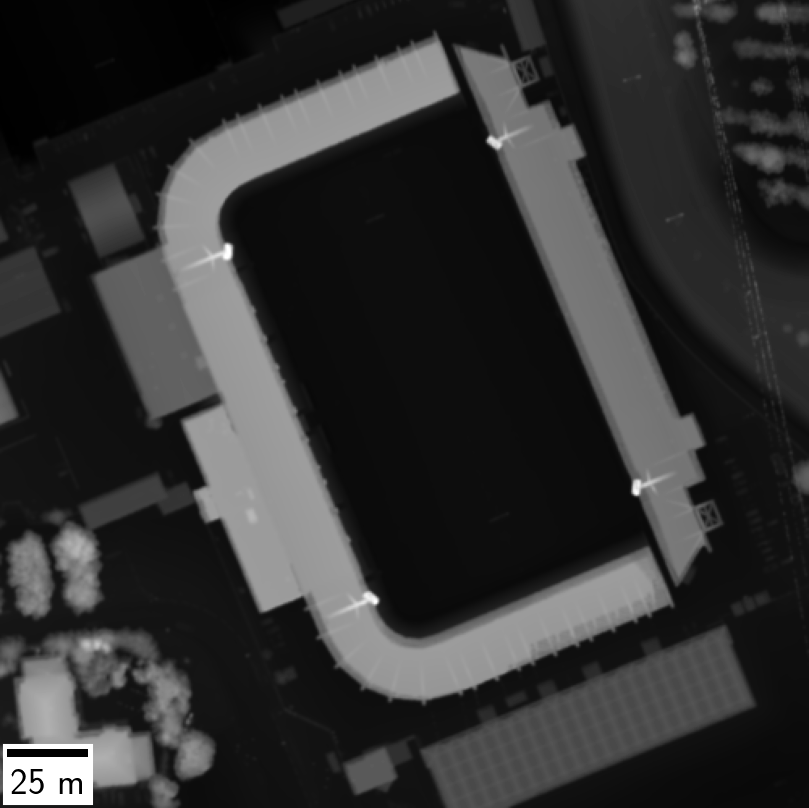
\includegraphics[height=6cm]{Images/Chap_1/DSM_Wallon_LiDAR.png}
        \caption{DSM from LiDAR HD data,\\Ernest Wallon stadium}
        \label{fig:DSM_ernest_wallon_lidar}
    \end{subfigure}\hfill
    \begin{subfigure}[t]{0.5\linewidth}
        \centering
        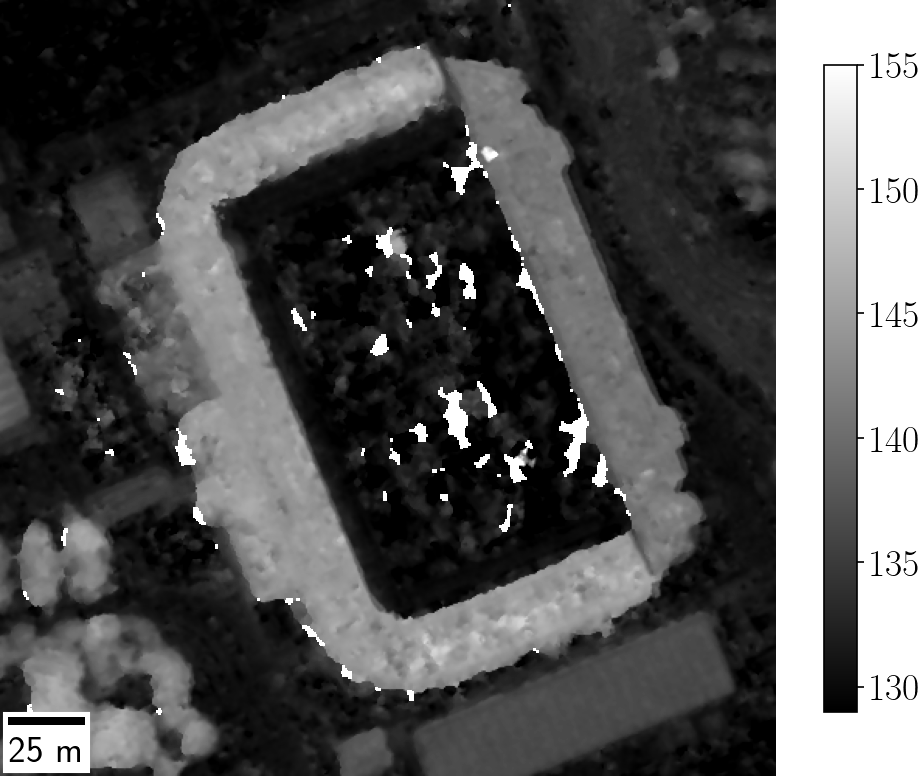
\includegraphics[height=6cm]{Images/Chap_1/DSM_Wallon_CARS.png}
        \caption{CARS DSM from Pléiades images,\\Ernest Wallon stadium}
        \label{fig:DSM_ernest_wallon_cars}
    \end{subfigure}
    \caption{Different DSM over Toulouse, France. DSM were obtained by rasterizing LiDAR HD data or by processing Pléiade stereo images with the CARS pipeline. The CARS pipeline uses a $5\times5$ CENSUS cost function and SGM regularization for stereo reconstruction. \copyright CNES 2017, Distribution AIRBUS DS}
    \label{fig:DSM_toulouse}
\end{figure}


Once the regularized cost volume $C_V^{SGM}$ has been computed, a simple \textit{winner-takes-all} strategy can be used to determine the disparity map $\mathcal{D}$:
\begin{align}
    \mathcal{D}(row, ~col) = \argmin_d C_V^{SGM}(row, col, d) 
\end{align}
\commanu{un peu court sur la stratégie de décision. rien à dire de plus sur l'état de l'art là dessus vu les échanges, et de perpectives? Peut etre juste une phrase du type: Winner takes all is the classical approach taken in literature but other approaches could be interesting to take especially with uncertainty information from this thesis.}

\subsubsection{Processing the Disparity Map}\label{sec:postprocess_disparity}
Once the disparity map has been computed, it is usually post-processed to remove artifacts, and improve disparity resolution.

It is common to add a sub-pixel refinement step, where a non-integer disparity is interpolated around the selected disparity. The main idea is to interpolate a model through the selected disparity $d=\argmin_\delta C_V(row, ~col, ~\delta)$ and its two direct neighbours\commanue{alors j'avais pas remarqué mais tu écris neighbors en anglais UK mais en général tu mets initialize donc c'est anglais US. Donc choisis ton côté de l'atlantique ;)}. The refined disparity $d_{interp}$ is then defined as the $\argmin$ of this interpolation model. \Cref{fig:sub-pixel_refinement} presents examples of interpolated disparities from  \cite{haller_real-time_2010}, mainly a ``V''-like shape as in \ref{fig:vfit_refinement} and a parabola as in \ref{fig:parabola_refinement}. Carrying out sub-pixel refinement suggests we assume the algorithm can attain a significant level of precision, which is debatable (see \Cref{sec:uncertainty_cars})\commanue{Et aussi que la fonction de coût a été suffisamment échantillonnée pour te permettre d'interpoler cotrrectement, ce qu'honnêtement on n'a jamais vérifié. On considère que c'est vrai}.

\begin{figure}
    \centering
    \begin{subfigure}[t]{0.5\linewidth}
        \centering
        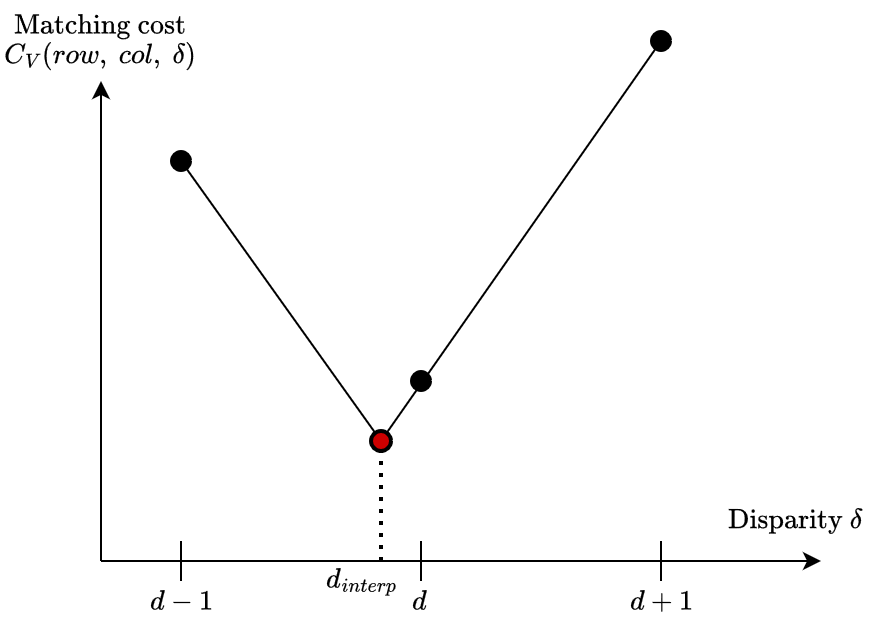
\includegraphics[width=\linewidth]{Images/Chap_1/subpixel_refinment_vfit.png}
        \caption{V-fit sub-pixel refinement}
        \label{fig:vfit_refinement}
    \end{subfigure}\hfill
    \begin{subfigure}[t]{0.5\linewidth}
        \centering
        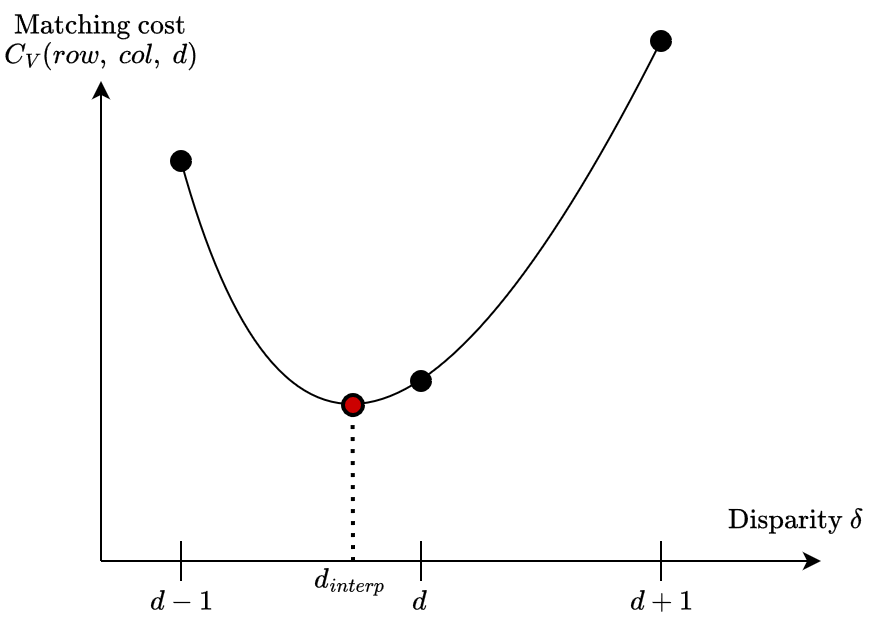
\includegraphics[width=\linewidth]{Images/Chap_1/subpixel_refinment_parabola.png}
        \caption{Parabola sub-pixel refinement}
        \label{fig:parabola_refinement}
    \end{subfigure}
    \caption{Different methods for refining the disparity $d=\argmin_\delta C_V(row, ~col, ~\delta)$}
    \label{fig:sub-pixel_refinement}
\end{figure}

The disparity map can also be filtered in order to remove local outliers. Classical strategies include the use of a mean or median filter for instance. There exists more advance filtering methods, such as bilateral filtering \cite{tomasi_bilateral_1998} which performs a weighted average, where weights depend on the proximity to other pixels both in the spatial and spectral domain.  

As presented previously, the \textit{winner-takes-all} strategy presents the inconvenient of allowing multiple pixels from the secondary image to be matched to the same pixel of the right image. For instance, if two pixels $(row,~col)$ and $(row,~col+1)$ from the second image have $d$ and $d-1$ as their respective disparity, they will be both matched to pixel $(row, ~col+d)$ in the reference image. This effect indicates that there is probably an error in the estimation of the disparity map. There exist strategies allowing to detect such error in order to eliminate dubious matches. A first strategy is called cross-checking \cite{fua_combining_1991}. We first start by computing a secondary cost volume $C_V'$ by reversing the roles of the images: the reference image becomes the secondary image and vice-versa. We then obtain two disparity maps $\mathcal{D}$ and $\mathcal{D}'$, and check that they are consistent, as in theory we would that $\mathcal{D}=-\mathcal{D}'$. A pixel $(row, ~col)$ is considered consistent across disparity maps if it verifies:
\begin{equation}\label{eq:cross-checking}
    |\mathcal{D}(row, col) + \mathcal{D}'(row, col+\mathcal{D}(row, col))|\leqslant \tau
\end{equation}
where $\tau$ is a consistency threshold usually set to $1$. For errors that do not check this consistency check, it has been proposed in \cite{hirschmuller_stereo_2008} to differentiate between mismatched pixels (pixels for which there exists a correct match) and occluded pixels (pixels that visible in an image but masked by an object in the other) as follows: if there is a disparity $d\in\mathcal{D}$ such that $\mathcal{D}'(row, col+d)=-d$ then it is a mismatch\commanue{la phrase est assez longue et en plus tu as des éléments en parenthèses. Il faudrait peut-être mieux splitter les éléments}. Otherwise, pixel $(row, ~col)$ is occluded. Occluded regions of an image can be filled by interpolation with the closest valid disparities\commanue{alors j'ai un doute on rebouche par interpolation avec les voisins les mismatch aussi, non?}.  

\begin{remark}
     \Cref{eq:cross-checking} requires the computation of a second cost volume, effectively doubles the processing time. As dense stereo matching is also the longest part of a photogrammetry pipeline, one might be reticent to carry out a cross-checking step. However, one might make the following observation: the cost volume contains the dissimilarity between every considered pair of pixels in the disparity range, so the cost of every considered match in the first cost volume is also present in the second cost volume. In theory, for every pixel $(row, ~col)$ and for every disparity $d$ in the (reference) disparity range, it holds \cite{bebis_mutual_2008}:
     \begin{align}\label{eq:diagonal_search}
         C_V(row,~col,~d) = C_V'(row,~col+d, -d)
     \end{align}
     \Cref{eq:diagonal_search} holds only for cost volumes obtained after the matching cost step. However, when SGM regularization or another aggregation cost method modifies cost volumes, then the there can be differences between $C_V(row,~col,~d)$ and $C_V'(row,~col+d, -d)$. In the case of SGM regularization, the differences between cost volumes are small and marginally modify the disparity maps. Using \eqref{eq:diagonal_search} then allow to obtain both cost volume by only computing one and re-indexing it to obtain the other. \todoroman{Ca c'est moi qui l'ait vérifié en faisant une batterie de tests https://confluence.cnes.fr/display/at3d/Faster+Right+Cost+Volume. J'ai pas trop de citations à fournir, est-ce que ça passe? Ou alors je le mets dans mes contributions.}\commanue{Tes contributions ce sont tes prez et articles. Là tu peux comme tu le mentionnes dire qu'après un ensemble de tests tu arrives à cette conclusion. Après Hirshmuller il se permet}
\end{remark}

\subsection{Triangulation}\label{sec:triangulation}
\commanu{une petite transition pour le lecteur, ca part direct sur le depth of a pixel sur une partie triangulation. rappelle peut etre l'objectif de la section et de l'étape métier.}
When working with pinhole camera models, the depth $z$ of a pixel is computed using the following formula:
\begin{equation}
	z=\frac{Bf}{d}\label{eq:z_bfd}
\end{equation}
where $B$ is the baseline between cameras, $f$ is the focal length of the camera, and $d$ is the disparity of a pixel. This formula can be found using optical geometry \cite{bolles_epipolar-plane_1987}, and illustrates the fact that pixels closer to the camera present a bigger position shift in between images\commanue{proposition mais vu comment les indiens ont corrigé mon doc je ne suis pas sure d'être une référence: pixels closer to the camera shift more significantly from one image to the other}. In the case of satellite imagery\commanue{Il me semble que tu l'as déjà dit donc j'ajouterais as mentioned previously au début de la phrase}, the pinhole camera model is not valid and we instead use other geometrical models\commanue{alors là ça fait traduction du français, je pense que sensor models est mieux} (see \Cref{sec:sensors_rpc}). \Cref{eq:z_bfd} thus cannot be used as such to provide accurate results.
\begin{remark}
    \Cref{eq:z_bfd}, although not used to determine the DSM, still provides an estimation of the height which can for instance used to determine the height of SIFT matches during the epipolar resampling step\commanue{C'est pas faux mais demandes-toi si il faut que tu gardes toutes les remarques. Je pense que celle-là tu peux supprimer}. \Cref{eq:z_bfd} also defines an important quantity, the $B/z$ ratio, usually called $B/H$ presented in \Cref{sec:epipolar_geometry}. This ratio is used to indicate the disposition of satellites\commanue{sensor positions} during the stereo acquisitions. A $B/H$ ratio near $0$ indicates a narrow angle between satellites\commanue{acquisitions car si tu n'as qu'un seul satellite...}, which will result in a DSM with few occluded areas but with low precision (an error of one disparity results in a larger height error)\commanue{Tu es comme Yannick un roi des parenthèses. Alors dans un manuscrit c'est pas un mail donc fait une autre phrase.}. Conversely, a higher $B/H$ ratio indicates a large angle between satellites\commanue{acquisitions}, resulting in a DSM with more occluded areas but with higher precision. In the case where one acquisition is made at nadir, the $B/H$ ratio equals the tangent of the angle formed between satellites views (see \Cref{fig:RPC}). For information purposes, the CO3D mission will provide acquisition with a $B/H$ ratio between $0.2$ and $0.3$.
\end{remark}

Instead, as RPC model\commanue{alors model c'est pour le verbe ou c'est RPC model le sujet et dans ce cas il te manque le verbe genre describe} every line of sight, we can use them to find the 3D coordinates of every match. To do so, first consider two stereo images, their RPC models $\RPC_1$, $\RPC_2$ from \cref{eq:rpc} as well as their epipolar grids $g_{e1}$, $g_{e2}$ from \cref{eq:epipolar_grid}. For every pixel $(row_e, ~col_e)$ from the reference epipolar image, whose disparity is $d$, then the 3D point $(X, Y, Z)$ represented by $(row, ~col)$ is the point verifying the following equations:
\begin{align}
    (X, Y, Z) &= \RPC^{-1}_1(g_{e_1}(row_e,~col_e),~Z)\label{eq:triangulation_exact}\\
    (X, Y, Z) &= \RPC^{-1}_2(g_{e_2}(row_e,~col_e+d),~Z) 
\end{align}
If the line\commanue{lines?} of sight intersect, then $Z$ is found by solving the following equation:
\begin{equation}
     \RPC^{-1}_1(g_{e_1}(row_e,~col_e),~Z) = \RPC^{-1}_2(g_{e_2}(row_e,~col_e+d),~Z) 
\end{equation}
Knowing $Z$ and $g_{e_1}(row_e,~col_e)$, \cref{eq:triangulation_exact} provides the $X$ and $Y$ coordinates as well.

\todoroman{En regardant le code de Shareloc, j'ai l'impression que chaque Line Of Sight est en fait une ligne droite lors de la triangulation. A verifier avec Manue/Manu/Loïc}\commanue{Alors je ne suis pas experte mais pour moi tu fais des segments car des RPC sont valides entre deux altitudes et ensuite tu cherches l'intersection ou le point le plus proche.}\commanu{dans shareloc, on a au départ un segment calculé sur  une alt min et alt max ou le RPC est valide mais transformé ensuite sur un starting point et viewing vector donc un point et un vecteur de direction donc une ligne pour la triangulation c'est bien ca qui est utilisé. donc ok avec description juste après, la référence de JMD est bien celle utilisé dans shareloc}
The problem is that lines of sight rarely present an exact intersection. By approximating line of sights by a starting point $P$, and a direction vector $\overrightarrow{V}$, we can instead define the coordinates $(X,Y,Z)$ as the point minimizing its distance two both lines. The exact formula for computing $(X,Y,Z)$ is provided in \cite{delvit_geometric_2006}:
\begin{equation}
    (X,Y,Z) = \left[ Id - V_1V_1^T + Id - V_2V_2^T \right]^{-1} \left[ (Id - V_1V_1^T)P_1 + (Id - V_2V_2^T)P_2 \right]
\end{equation}
where $Id$ is the identity matrix, and $V^T$ is the transposed vector $V$.

Triangulating every point using the disparity map leads to a 3D point cloud. Because we know from which pixel each 3D point originates from, we can associate to every 3D point additional information such as:
\begin{itemize}
    \item The color of the reference pixel (if provided). The point cloud is thus a colored point cloud.
    \item Confidence measures computed during the dense-matching step\commanue{Oui c'est vrai mais tu n'as jamais mentionné les mesures de confiance}. 
\end{itemize}

The 3D points can be filtered to remove obvious errors. Two different filtering\commanu{c'est quand meme bizarre de garder triangulation et filtrage dans la meme section. Si tu parles de filtrage (est ce utile ?), fais une sous section, je pense} steps are carried out: one for removing statistical outliers, and one for removing so-called ``small-components''\commanue{Alors ça c'est les filtrages de CARS}. 
\subsubsection{Statistical outliers filtering}
Points that are statistical outliers, are determined by considering the positions of its neighbours. For each point $P$, we compute the mean distance $\mu_P$ to its $N$ neighbours. Then we can compute for each point $P$ the mean distance $\mu$ and standard deviation $\sigma$ of its $N$ neighbours as:
\begin{align}
    \mu &= \frac{1}{N}\sum_{i=1}^N\mu_i\\
    \sigma &= \sqrt{\frac{1}{N-1}\sum_{i=1}^N(\mu_i-\mu)^2}
\end{align}

A point $P$ is considered to be a statistical outlier if its mean distance $\mu_P$ its far away from the mean distance of all of its neighbours according to the following criterion:
\begin{align}
    \mu_P>\mu+k\sigma
\end{align}
Where $k$ is a constant set by the user, usually set to $5$. We also consider $N=50$.

\subsubsection{Small-components filtering}
The other filtering method, named small-components filtering, attempts to remove small isolated clusters of points. For each point, we count the number of neighbours $N$ present within a distance $D_{max}$. If this number is inferior to a given threshold $N_{min}$, then we consider the point belongs to a small component and is removed. Formally, a point $P$ is removed if:
\begin{align}
    \#\{~\text{Points } Q~|~\sqrt{(P-Q)(P-Q)^T}\leqslant D_{max}~\}\leqslant N_{min}
\end{align}
We usually set $D_{max}$ to $3m$ and $N_{min}$ to $50$.

\Cref{fig:point_cloud_filtering} illustrates the two filtering methods presented. More advanced filtering methods can be implemented, such as bilateral filtering \cite{digne_bilateral_2017}, and filtering using color information or confidence measures from the disparity map (see \Cref{sec:uncertainty_pandora}) \cite{youssefi_geometrically_2024}\commanue{je mettrais ce paragraphe plus haut quand tu mentionnes les filtres de CARS et avant de les décrire en détail}.

\begin{figure}
    \centering
    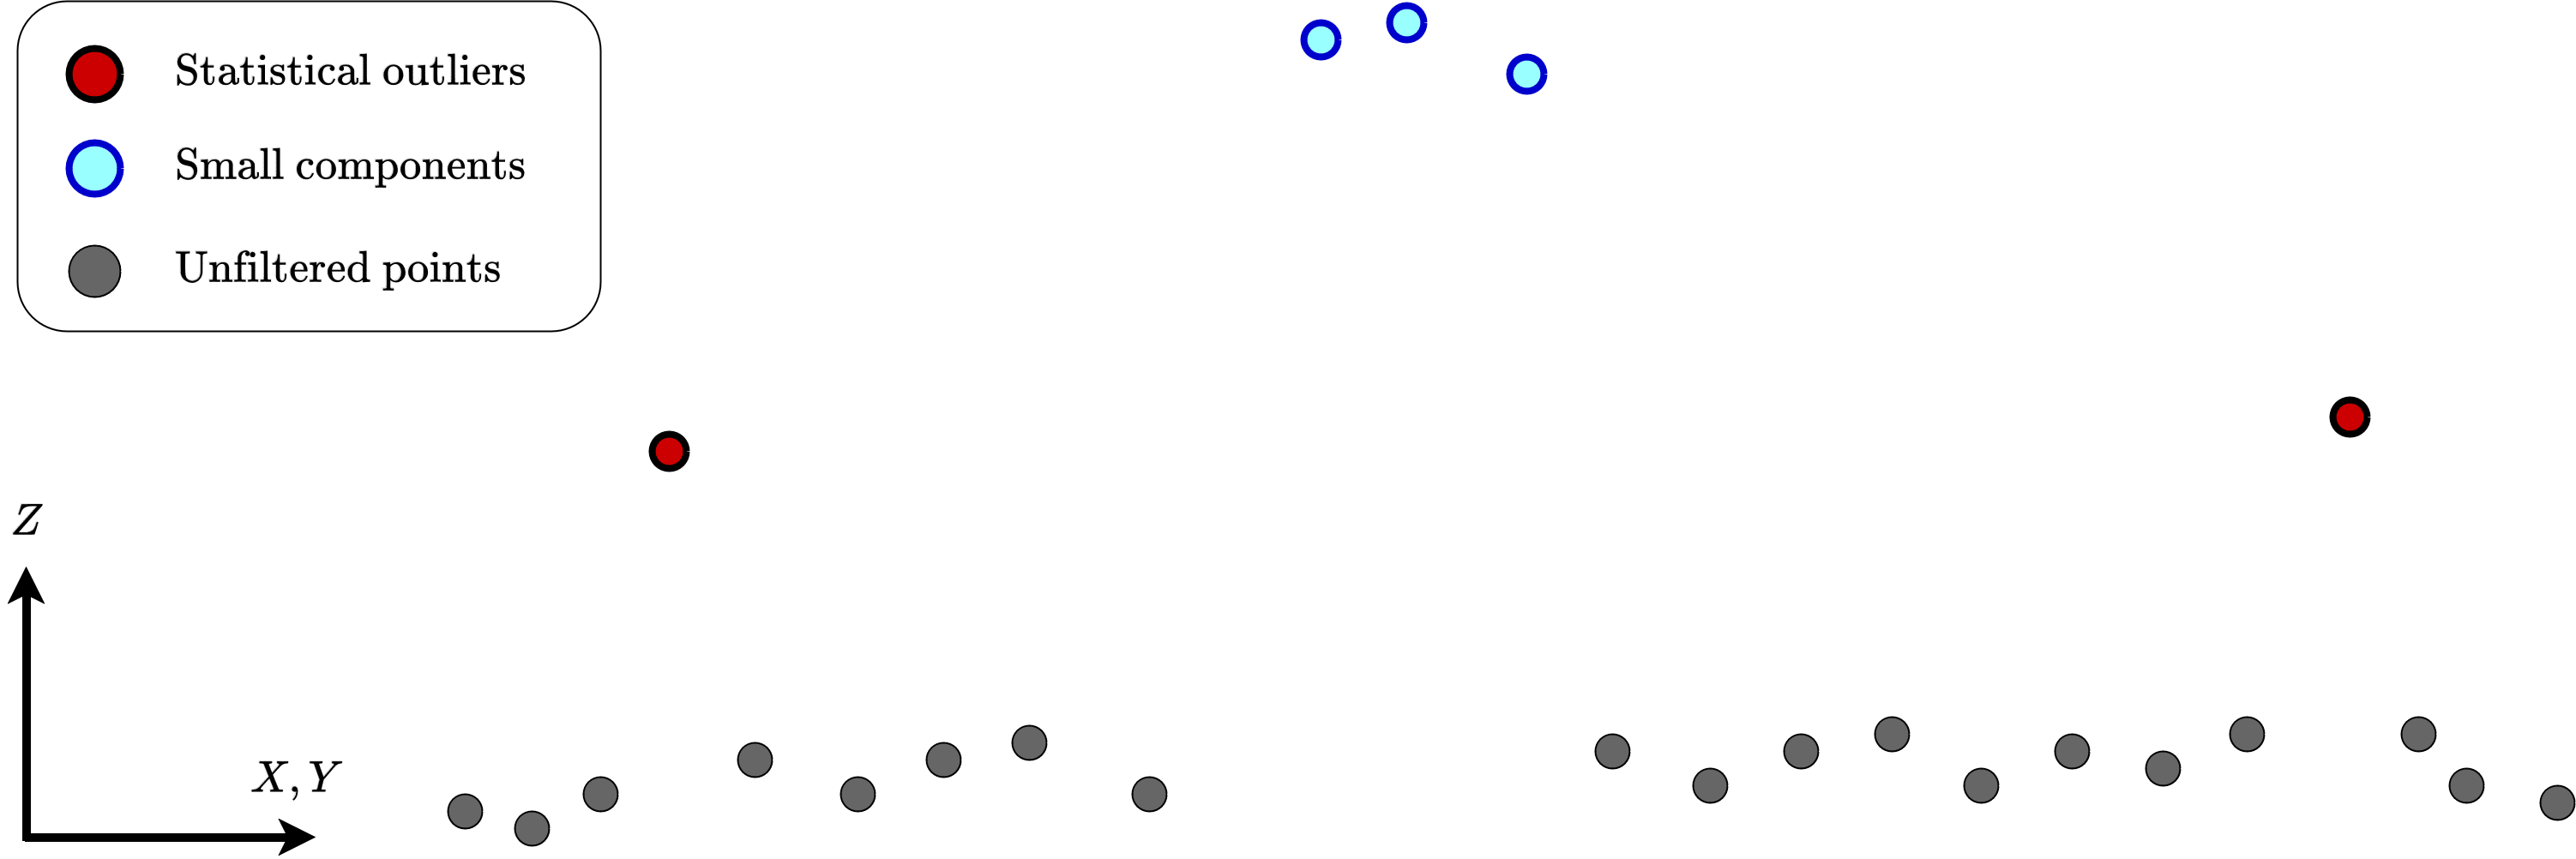
\includegraphics[width=\linewidth]{Images/Chap_1/Point_cloud_filtering.png}
    \caption{Example of statistical outliers and small components filtering of a 3D point cloud.}
    \label{fig:point_cloud_filtering}
\end{figure}

Filtering the point cloud results in a 3D product that can already be provided as such to users. However, point clouds, while containing more 3D information than DSM, can be hard to manipulate in conjunction with other \acrshort{gis} data. Projecting the point cloud on a regular grid to produce a DSM is thus often preferred, which constitutes the final step of the stereo pipeline.

\subsection{Rasterization}\label{sec:rasterization}
Rasterization consists in projecting the 3D points onto a regular grid over the $(X,Y$) plane to produce the final DSM. One of the challenges faced when projecting the point cloud is that of the relative\commanue{low?} density of the point cloud relative to the DSM grid. Indeed, if the density of the point cloud is high enough, multiple 3D points can be projected to the same cell, which raises the question on how to merge their 3D information. On the other hand, if the density is low enough\commanue{loo low?}, there may some cells where no points are projected onto. 

The CARS stereo pipeline uses a Gaussian interpolation to fuse the information of point clouds. Given a cell with coordinates $(X,Y)$ of the DSM, we consider every point $P_i=(X_i, Y_i, Z_i)$ in a given radius $r$ of $(X,Y)$, and note $\mathcal{N}_{XY}$ the set of all those points. The final value of the DSM is then computed as the following mean with Gaussian weights:
\begin{align}
    DSM(X,Y) &= \frac{\sum_{P_i\in\mathcal{N}_{XY}}Z_i\cdot e^{-\frac{(X_i-X)^2+(Y_i-Y)^2}{2\sigma^2}}}{\sum_{P_i\in\mathcal{N}_{XY}} e^{-\frac{(X_i-X)^2+(Y_i-Y)^2}{2\sigma^2}}}
\end{align}
with sigma usually set to $0.3m$ and the radius $r$ being $3m$. \Cref{fig:rasterization} illustrates the rasterization process.

Rasterizing with this method presents\commanue{provides/offers pour éviter la répétition de present} the advantage of smoothing the potential height variations still present in the 3D point cloud, while allocating more weight to points that are near the cell center. This method can also be found in other stereo pipelines \cite{shean_automated_2016}, while other pipelines use different weighting methods, such as Inverse Distance Weightings (IDW) \cite{rupnik_micmac_2017}, producing similar results.

\begin{figure}
    \centering
    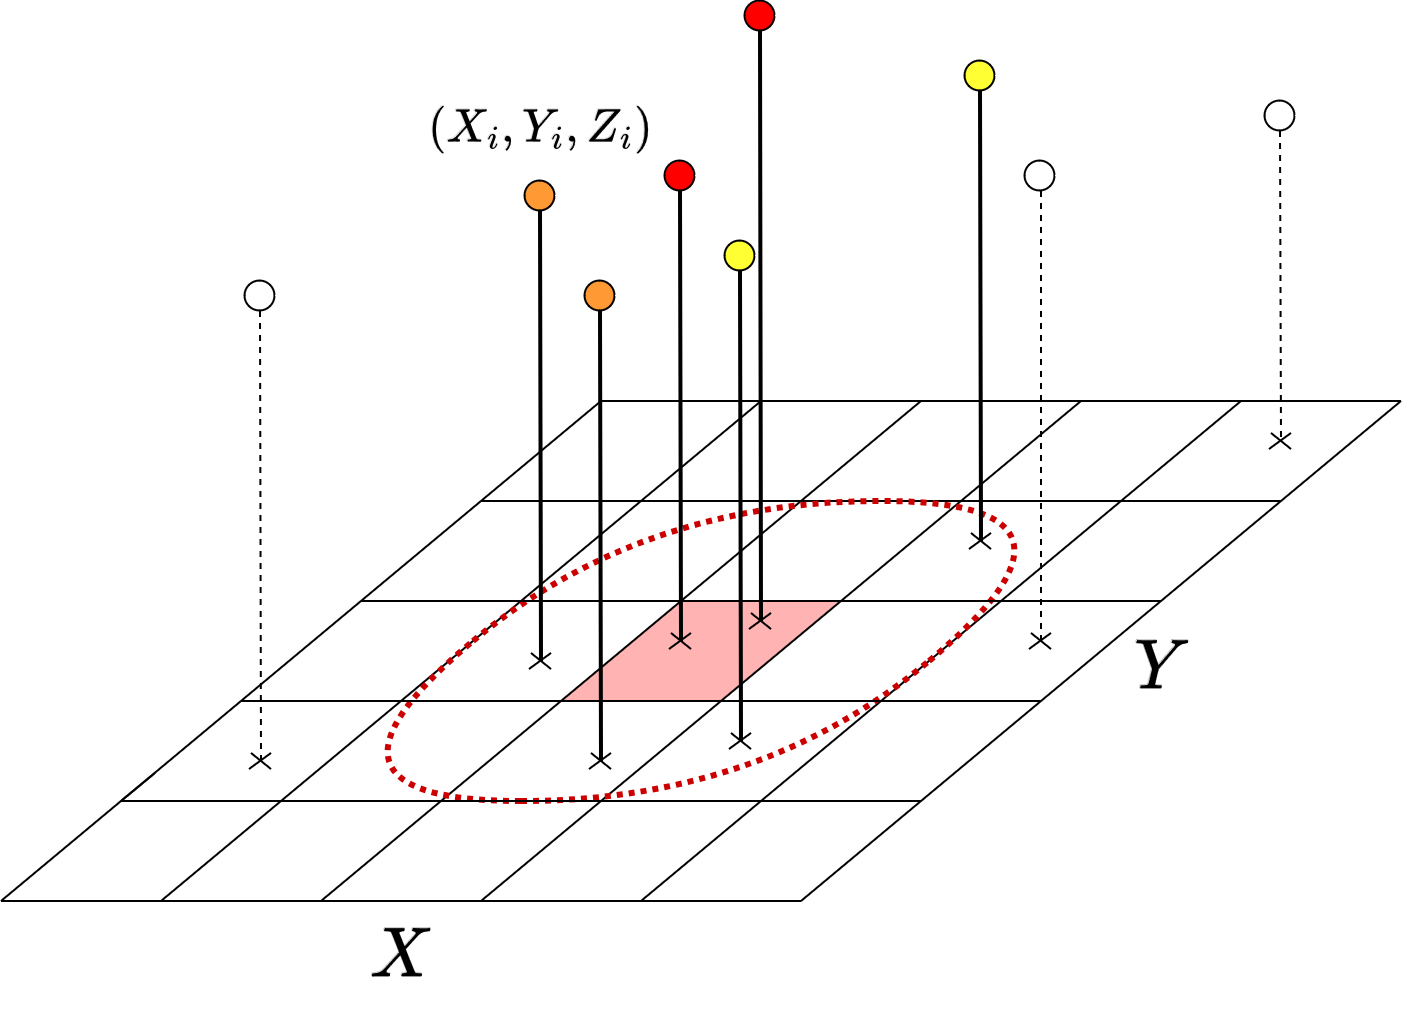
\includegraphics[width=0.7\linewidth]{Images/Chap_1/Rasterization.png}
    \caption{Rasterization of the point clouds on a regular grid. Red points are nearer to the center $(X,Y)$ of the considered cell, while yellow points are further away.}
    \label{fig:rasterization}
\end{figure}

\begin{remark}
    If no points are projected in a given cell (or its direct neighbours), then the cell can be filled with \textit{nodata} values. Different method can be considered to fill holes, such as directly using the values of nearest valid neighbouring cells, or interpolating their values. More advanced methods consists in simulating a cloth-like surface fill the holes as in \cite{lallement_bulldozer_2022}.
\end{remark}

\subsection{From LiDAR to Ground Truth Disparity}
\commanu{bizarre dans la section stereophotogrammetry pipeline. C'est plus pour la qualification. T'as vraiment besoin d'expliquer ou tu peux juste citer dans ta partie résultats quand tu abordes la qualification ? tu verras si ca saute pas du coup. Moi j'enleverais d'ici, ca n'a pas vraiment sa place, je trouve}
Parler du LiDAR HD en général. 

Explaination on how to obtain GT disparity maps from georeferenced LiDAR, \cite{cournet_ground_2020}. Line of sight and default geoid. 

\section{Uncertainty in Stereophotogrammetry}\label{sec:previous_work_stereo_uncertainty}
\todoroman{Sources d'incertitudes : acquisition des images et bruit sur le capteur. Précision du model RPC. Incertitude issue des différentes traitement (rééchantillonage, stereo matching). Intersection des lignes de visée. Rasterization.}
\commanu{du coup intro de la section à faire pour comprendre le déroulé ensuite}
\commanu{bien mettre en avant quelque part début ou fin de la section qu'il y a peu de travaux sur le sujet et que donc ton travail est novateur et défriche quelque chose de peu regardé. Remarque des implémenteurs de Mic Mac: c'est trop complexe. donc mettre quelque chose qui donne ce recul au lecteur et qui explique qu'il n'y ait pas bcp de travaux cités. Ce n'est pas un raté de ton travail d'état du lard!}
\subsection{Previous work}
\commanu{titre: on dirait que c'est ton travail précédent. Plutot state of the art?}
\todoroman{Regarder ce qui se fait sur les autres produits 3D: BD ALTI \url{https://geoservices.ign.fr/bdalti}, section 2.2.2 \url{https://geoservices.ign.fr/sites/default/files/2021-07/DC_RGEALTI_2-0.pdf}. Mission Copenicus avec WorldDEM par TandDEM X \url{https://fr.wikipedia.org/wiki/TanDEM-X}}

The quality of \acrshort{dsm} obtained using stereophotogrammetry can greatly vary depending on the quality/resolution of the images used, the precision of the geolocation, the performances of the stereo matching algorithm \etc. Reducing the magnitude of errors, or evaluating the uncertainty \textit{a posteriori} has been investigated in multiple work.
Uncertainty on \acrshort{dsm} has been mainly evaluate using a single confidence interval over the whole DSM \cite{hugonnet_uncertainty_2022, deschamps-berger_apport_2021, wang_robust_2015, oksanen_digital_2006,panagiotakis_validation_2018}. Intervals are computed based on a set of reference points, either extracted from a better resolution \acrshort{dsm}, or ground truth data. \todoroman{Reprendre le papier où ils samplent depuis leur prorpre DSM}. Fusing \acrshort{dsm} to get better accuracy \cite{qin_uncertainty-guided_2022}
\cite{hu_quantitative_2012,poggi_confidence_2021}
Deep uncertainty for disparity?

The ASP pipeline\commanu{je remettrais: The NASA's ASP pipeline cited before... } can take as inputs camera standard deviation of position uncertainty (expressed in meters) in the horizontal ground plane, and propagate it during the triangulation and rasterization steps. The documentation (\url{https://stereopipeline.readthedocs.io/en/stable/error_propagation.html}) details the covariance matrix propagation method used. It explicitly states that the propagated uncertainty does not represent the error between the predicted height and a hypothetical ground truth, even though they are expressed in the same unit of measure. It is rather the propagated covariance from the camera position projected in the horizontal and vertical directions, regardless of the matching errors or triangulation error if the line of sight do not intersect.

\subsection{Uncertainty in the CARS pipeline}\label{sec:uncertainty_cars}
In this thesis, we focused on quantifying the uncertainty alongside the creation process of \acrshort{dsm}. We thus differ in this regard from previous work, which produces a single confidence intervals from the final produced DSM. Multiple sources of uncertainty influence the production of a DSM, which we will now detail\commanu{proposition: I will now detail the multiple sources of uncertainty that influence the DSM production. remarque tjrs sur I et we, choisis et sois cohérent sur l'ensemble}.

First, the images contain noise from the captor\commanue{sensor?}, and some atmospheric effects may appear on the acquisitions. For push-broom sensors, satellite movements can have a big impact on the final images. For instance, vibration of the satellite that are not taken into account in the geometric model can lead to biases on the geolocation of the different rows of the image. Those biases will themselves be propagated to the final DSM. Those are the main uncertainties associated with the input data.\commanu{en gros tu aurais des effets sur la radiométrie (pas forcément que le bruit et l'atmosphère, ca peut etre compression ou autre artefact dans la production, je suis pas expert mais quasi sur que plein de choses...) et la géométrie (pas forcément que les vibrations, ca peut etre un mauvais calage, une mauvaise référence, je dirais qu'il y a plus que les vibrations, voir daniel). Bref, tu dois pouvoir généraliser en "radiométrie" et "géométrie" pour etre plus juste, tout en citant en exemple ce que tu as mis. A mon avis, l'analyse d'incertitude sur ces "input data" pourrait etre une thèse en soi, donc un peu court}

Other errors occur when processing this data. First, different resampling\commanue{several resamplings?} occur in order to convert stereo images from captor\commanue{alors captor je ne suis pas fan je mettrais sensor} geometry to epipolar geometry. Those resamplings introduce errors if the input and target resolutions do not respect Shannon criteria \cite{delon_small_2007} \todoroman{mettre les formules? affiner la phrase}. Moreover, the sparse matches used to refine the epipolar grid heavily\commanue{strongly?} depend on the performance of the SIFT algorithm used to obtain them. In similar terrain, for instance on glaciers where many homogeneous region are present, some false matches can be observed. This leads to wrong epipolar lines, and those errors will themselves be propagated in the following steps of the pipeline\commanue{Oui on a aussi un problème sur des champs où l'alignement n'était pas bon. Après je pense que c'est surtout qu'avec les SIFTS parfois on trouve pas le bon intervalle...}. Those errors are usually minor, compared to those occurring in the dense stereo matching step\commanue{Ah bah voilà c'est forcément la faute de pandora. David et Dimitri ont trop déteint sur toi ;)}.

Dense stereo matching is a complex task, for which many different algorithms exist, each potentially presenting different performances. Using a window-based correlator with SGM regularization usually presents good performance in areas without height discontinuities. This can become a problem in urban areas, where the presence of high buildings represents an additional challenge for the correlator. Because the correlator compares windows ($5\times5$ using the CENSUS cost function or $11\times11$ using MC-CNN) and not single pixels, this naturally creates an adherence effect near building borders\commanue{Alors moi j'ai lu les différentes versions de ce chapitre donc là il faut peur-être faire un renvoi à l'adhérence}. Note that in \cite{okutomi_stereo_1994}, authors have been trying to adapt the window shape to reduce the uncertainty of stereo matching, but this method requires to iteratively compute costs on different windows, which can become quite expensive. SGM regularization also penalizes disparity changes, thus reinforcing the adherence effect. Other processes, such as filtering or sub-pixel refinement, improve the quality of the disparity map but require specific care for handling their induced uncertainty. Sub-pixel refinement also supposes that sub-pixel disparities can be deducted without upsampling the input images, which is debatable\commanue{C'est plutôt qu'on ne vérifie pas que la fonction de coût est suffismament échantillonnée et effectivement si ce n'était pas le cas il faudrait suréchantillonner l'image, là tu me fais un peu la version raccourcie}. The dense matching step is crucial as previous errors usually have a smaller impact on the final product than the errors potentially occurring in stereo-matching\commanue{Même si la phrase me rend triste il faudrait la mettre en début du paragraphe, elle est importante et te fera le lien avec avant. D'ailleurs tu peux mettre aussi le reste du paragraphe avant.}. For instance, a bias in the epipolar grid typically leads to a shift of one row between the epipolar images. This leads to typical errors of around $1$ disparity. In comparison, the correlator can produce errors with a magnitude of the whole disparity research interval, sometimes reaching values near $100$ disparities. Considering those orders of magnitude, estimating and quantifying the uncertainty of the stereo-matching process is crucial to control the uncertainty on the output DSM. \Cref{sec:uncertainty_pandora} dives more into details regarding the different methods that have been developed to quantify the uncertainty of dense stereo matching.

Once the disparity has been estimated, 3D points can be triangulated by intersecting RPC lines from each matched pixel. However, we saw previously that there is no guarantee that the 3D lines do intersect. If they indeed do not intersect, the 3D point is defined as the point minimizing its squared distances to both lines of sight. An alternative is to modify the geolocation line from the secondary image so as it intersects the line from the reference image. In both cases, the localization of the 3D point is not exact. This uncertainty stems from the fact that we determine the 3D coordinates of the point from a match between two pixels that do not point exactly to the same object\commanue{Je comprends ce que tu veux dire mais il faudrait voir si on peut pas améliorer la formulation. Avec l'échantillonnage des pixels les pixels ne sont pas exactement comparable. Je réfléchis à comment le reformuler}. Additionally, RPC models attempt to represent real lines of sight with polynomial coefficient, which is not exact and possess its own accuracy. The method used for coefficients calibration and the frequency of calibration also bring their share of uncertainty.

The final part of the stereo pipeline is to rasterize the point cloud onto a regular grid, thus yielding the DSM. When characterizing the uncertainty on the final result, we must first agree on what the DSM is supposed to represent. It is common to consider that each pixel's value should represent the average height over the cell. However, providing the maximum or minimal height might be more adapted to some scenarios: for instance if the DSM is used to prepare very low altitude flights (for drones \etc), the maximum height is more relevant as one would want to avoid any foliage or power line. Those elements could disappear in the fin\commanue{clairement il manque la fin ;)}. In this thesis, we will consider that the DSM represents the (weighted) average height. The weights considered will be computed with a Gaussian whose variable is the distance to the center of the cell\commanue{Remarque un peu globale mise à l'arrache ici, mais il faudrait relire quand tu auras fini la partie d'avant pour voir si ça ne fait pas trop redite avec la description du pipeline}. Other weights can be considered, most notably the \textit{inverse distance weighting} (IDW), which produces very similar results in our applications. We now specified the projection method\commanue{Pourquoi au passé?}. Depending of the resolution of input images and the desired output resolution of the DSM, the density of points per DSM cell will vary. In our applications, the input and output resolutions are identical as we typically desire to produce a DSM at $50$cm resolution from $50$cm panchromatic images. This means that there is on average one 3D point per DSM cell. For occluded regions, or when we discarded stereo matches that seemed wrong, there might be no point directly in the output cell. In this case, the value of the DSM cell will be completely determined by the value of points in neighbouring cells, even if their distance is high and the averaging weights are small. Interpreting the final DSM as the average height on each cell is thus debatable, as the average is computed on a limited number of points, and sometimes not even belonging to the considered cell.  Note that if there is no points around in a given radius, the cell will be left empty. 

Different sources of uncertainty occurring throughout the stereo pipeline were presented in the previous paragraphs. Characterizing, modelling and propagating all of those uncertainties could not be considered in the span of this thesis. We thus focus mostly on the uncertainty arising from the dense stereo matching step, as it is the source of the biggest errors in the pipeline. \Cref{chap:propagating} investigates how uncertainty from the input epipolar images can be propagated in the stereo matching step, and \Cref{chap:epistemic_uncertainty} attempts to model the processing uncertainty of stereo algorithm itself. We also propagate this uncertainty all the way to the output DSM and show that it can correctly estimate the errors made during the DSM production. 

We conclude this section with a small disclaimer: our methodology estimates the uncertainty independently for every pixels, leading to small confidence intervals in confident areas, and bigger confidence intervals where the algorithms may have performed badly. We differ in this regard to the methods presented in \Cref{sec:previous_work_stereo_uncertainty}, which estimate a single global confidence interval \textit{a posteriori}, based solely on the DSM (and reference points), regardless of the method used to obtain it. In this regard, it does not seem relevant to compare our intervals to theirs, as there most similar characteristics is their name ``interval'', but neither share the same form (single \vs multiple intervals), nor are based on the same data. \commanu{je me demande si tu peux pas mettre cette dernière partie dans une sous section à part. Ce ne serait donc pas un disclaimer mais une présentation  Cette sous section (et la suivante sur le dense matching) décrit les sources d'incertitude que tu vois et pourrait amener à une sous section de transition ou tu expliques et justifies les choix pris pour la thèse vers le chap 4 et 5 en disant que l'idée était de prendre aussi les techniques méthodologiques du chap 2 et 3 en considération. }

\subsection{Uncertainty Quantification in Dense Stereo Matching}\label{sec:uncertainty_pandora}
As stereo-matching is a popular problem in computer vision, many methods for quantifying its uncertainty have been proposed in the literature. Without being exhaustive, this section presents a quick overview of the main approaches as well as the solutions currently implemented in the dense stereo correlator Pandora used in the CARS pipeline.

The way uncertainty is quantified in stereo matching is by producing \textit{confidence maps}, \ie a mapping for each pixel $(row, ~col)$ to a real confidence value, usually between $0$ and $1$. By convention, a value of $0$ means that we are not confident in the disparity value associated to $(row, ~col)$. Conversely, a confidence value of $1$ indicates that we are very confidence in the predicted disparity.

\begin{remark}
    \todoroman{Faire relire cette remarque à Manue et Seb car je l'ai écrite après leur relecture }It is interesting to see that in \cite{quinio_random_1992}, the author considered using closed random sets (a concept related to imprecise probabilities and belief functions studied in \cref{chap:representation_of_uncertainty} \cite{quinio_random_1991}) to model the uncertainty of a stereoscopic setup. They mainly consider the uncertainty arsing from the limited resolution of digital images (as we do in \cref{chap:propagating}), and from the precision of the calibration setup: focal length of cameras, baseline distance, orientation and vengeance angle of the cameras \etc. They consider that the uncertainty from dense matching is not of epistemic nature, but of aleatoric nature, and thus do not model it by imprecise models as we do in \Cref{chap:epistemic_uncertainty}. This hypothesis is justified as they achieve the stereo matching step using a window based ZNCC cost function (without \acrshort{sgm}, as it was not published at the time), which by nature possess strong links with probabilistic models.
\end{remark}

There are multiple sources of information that can be used to compute a confidence measure. Left and right input images and the predicted disparity map being those available to every method, but cost-based approaches can also make use of the cost volume, as it contains a lot of useful information. Most confidence measures were first handcrafted using those different information sources. For reviews on those methods, we refer to \cite{egnal_stereo_2004, hu_quantitative_2012, poggi_quantitative_2017}. With the rising use of deep-learning in stereo, many networks have been developed to estimate the uncertainty. A review for methods using regression forests can be found in \cite{min-gyu_park_leveraging_2015}, and a more general review, including the use 2D and 3D CNNs on the cost volume, can be found in \cite{poggi_confidence_2021}.

\begin{remark}
     Quantifying the uncertainty in stereo matching is a popular field of research. Recently, people have even been trying to evaluate the uncertainty of the confidence estimation itself, called \textit{meta-confidence} \cite{kim_meta-confidence_2022}.
\end{remark}

\begin{example}
    Let us present some examples of confidence measures that use different sources of information.\commanue{Pourquoi tu ne mets pas cette phrase à l'extérieur de l'encart, afin de ne pas avoir l'encart qui poppe. Après je ne sais pas au final si un encart est nécessaire.}
    
    Regarding confidence measure based on the disparity map, we already presented a type of binary confidence measure in \Cref{sec:postprocess_disparity} with the cross-checking test from \cref{eq:cross-checking}. Other methods compute for instance the local variance of the disparity map, where a low variance suggests confident regions.
    
    For methods using the cost volume, a simple method for measuring the cost would be using the value of the matching score measure (MSM, \cite{egnal_stereo_2004}) for a given disparity at coordinates $(row, ~col)$:
    \begin{equation}
        MSM(row, ~col) = -C_V(row, col, \mathcal{D}(row, ~col))
    \end{equation}
    This measure can be normalized between $0$ and $1$ using the global minimum and maximum of the cost volume. The idea behind this measure is the following: a high matching cost for a selected disparity indicates that the two matched pixels are not that similar, and thus the match is not confident. Other measures using the matching cost compare the value of the first and second minimum of a cost curve, or measure the curvature of the cost curves. More advances measures make use of 3D CNNs on the entirety of the cost volume to learn an efficient confidence measure \cite{mehltretter_cnn-based_2019}.
    
    Measures based on the input images usually measure the gradient \cite{haeusler_ensemble_2013} or variance \cite{park_learning_2019} of input images. High gradient or high variances indicate highly-textured regions, which are often easier to match. The confidence is therefore higher for those pixels. 
    
    Deep-learning approaches can combine multiple sources of information (input images, cost volume, disparity map) to learn a confidence measure \cite{tosi_beyond_2018, kim_adversarial_2020}.
\end{example}

In this thesis, we will also consider three confidence measures that can already be computed with our correlator. Those measures will help us to quantify the uncertainty in the photogrammetry pipeline or will be used as comparison with our proposed method.

\begin{figure}
    \centering
    \begin{subfigure}[t]{0.5\linewidth}
        \centering
        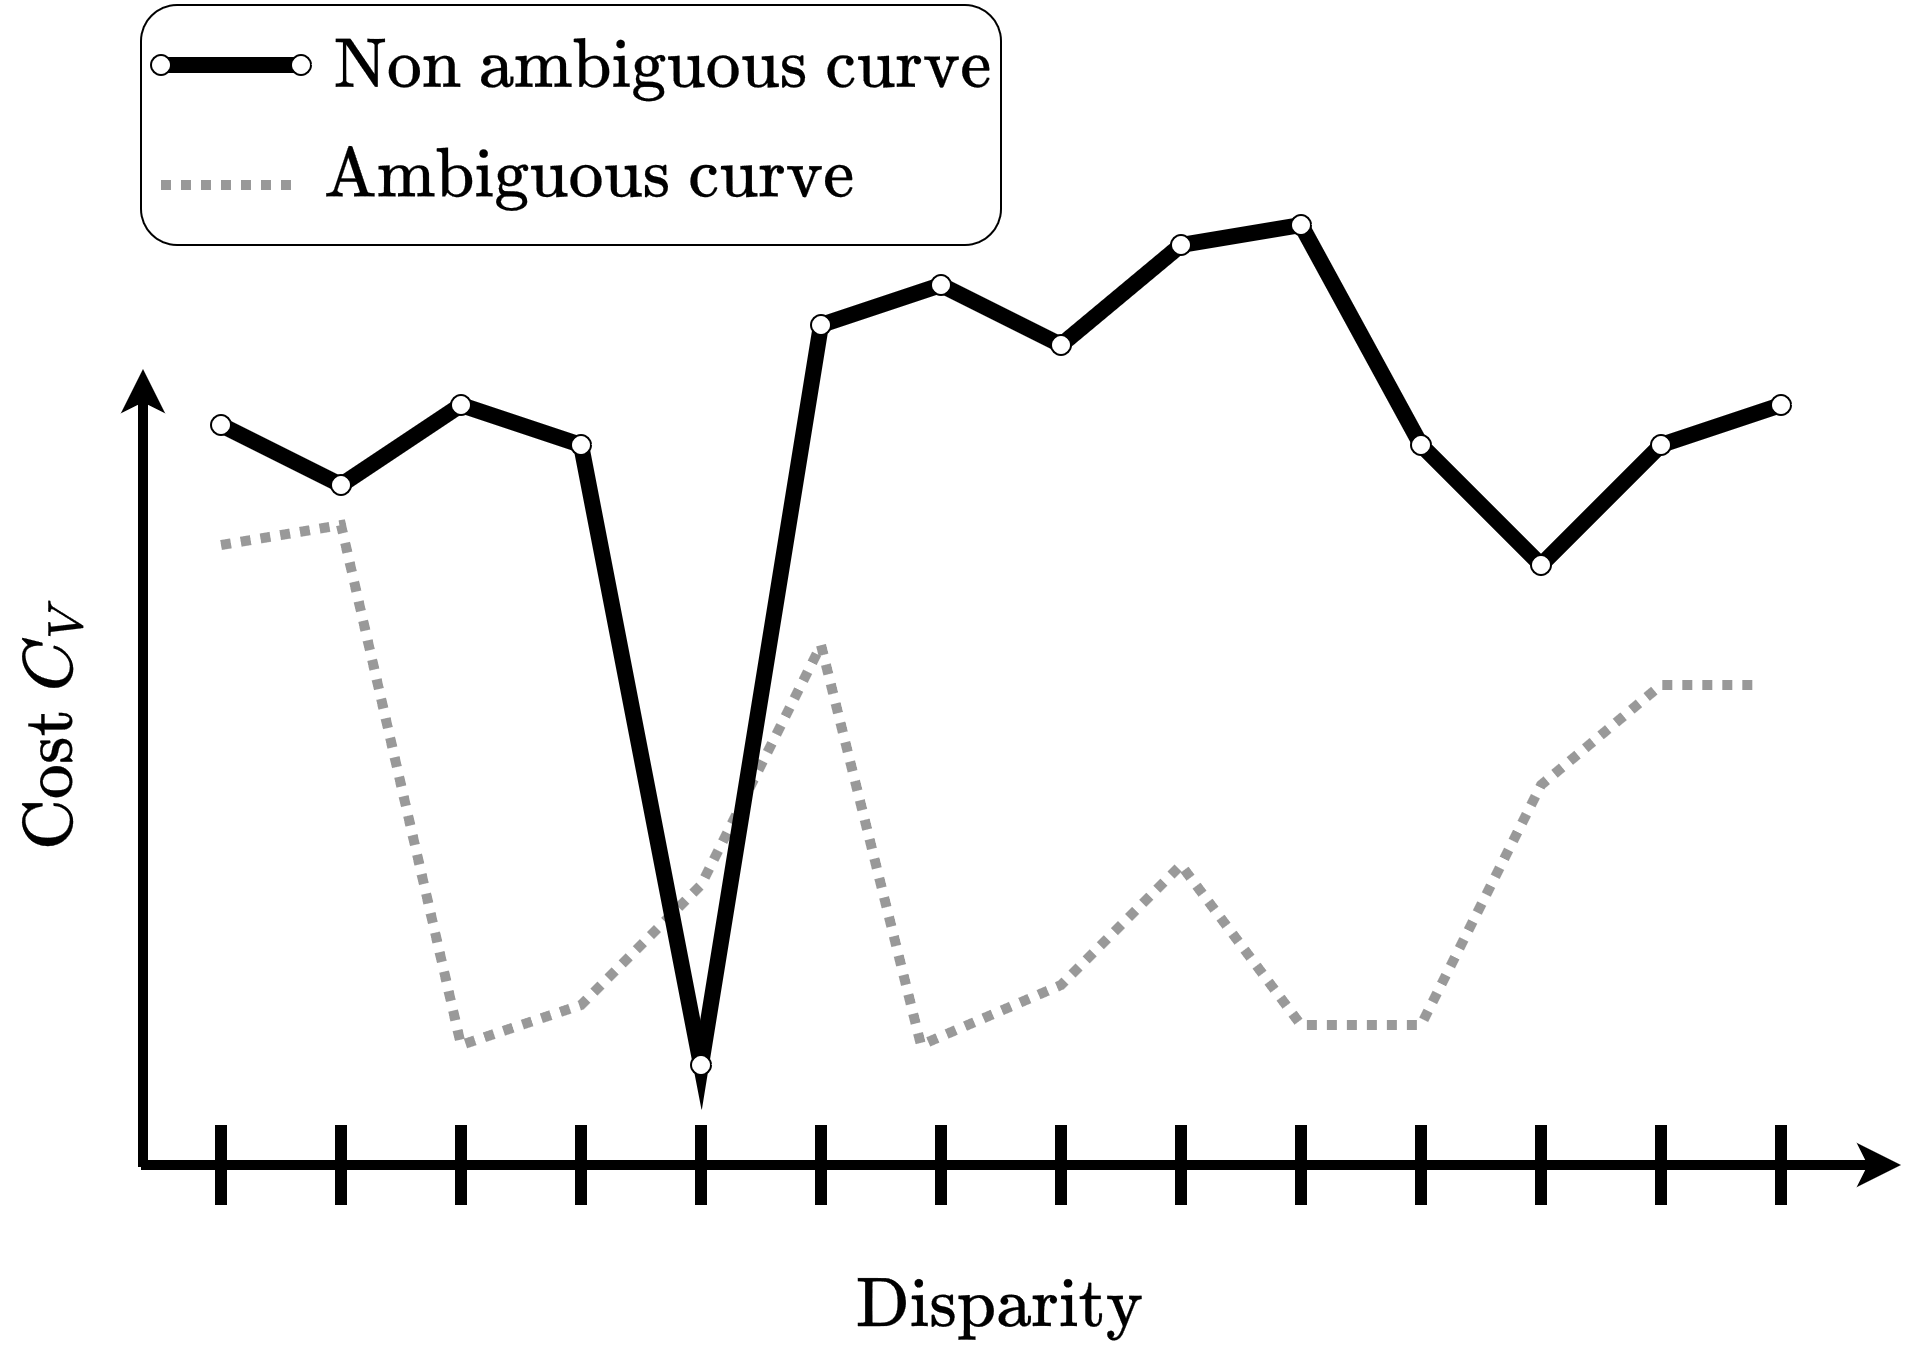
\includegraphics[width=\linewidth]{Images/Chap_1/Ambiguity.png}
        \caption{}
        \label{fig:ambgiuity}
    \end{subfigure}\hfill
    \begin{subfigure}[t]{0.5\linewidth}
        \centering
        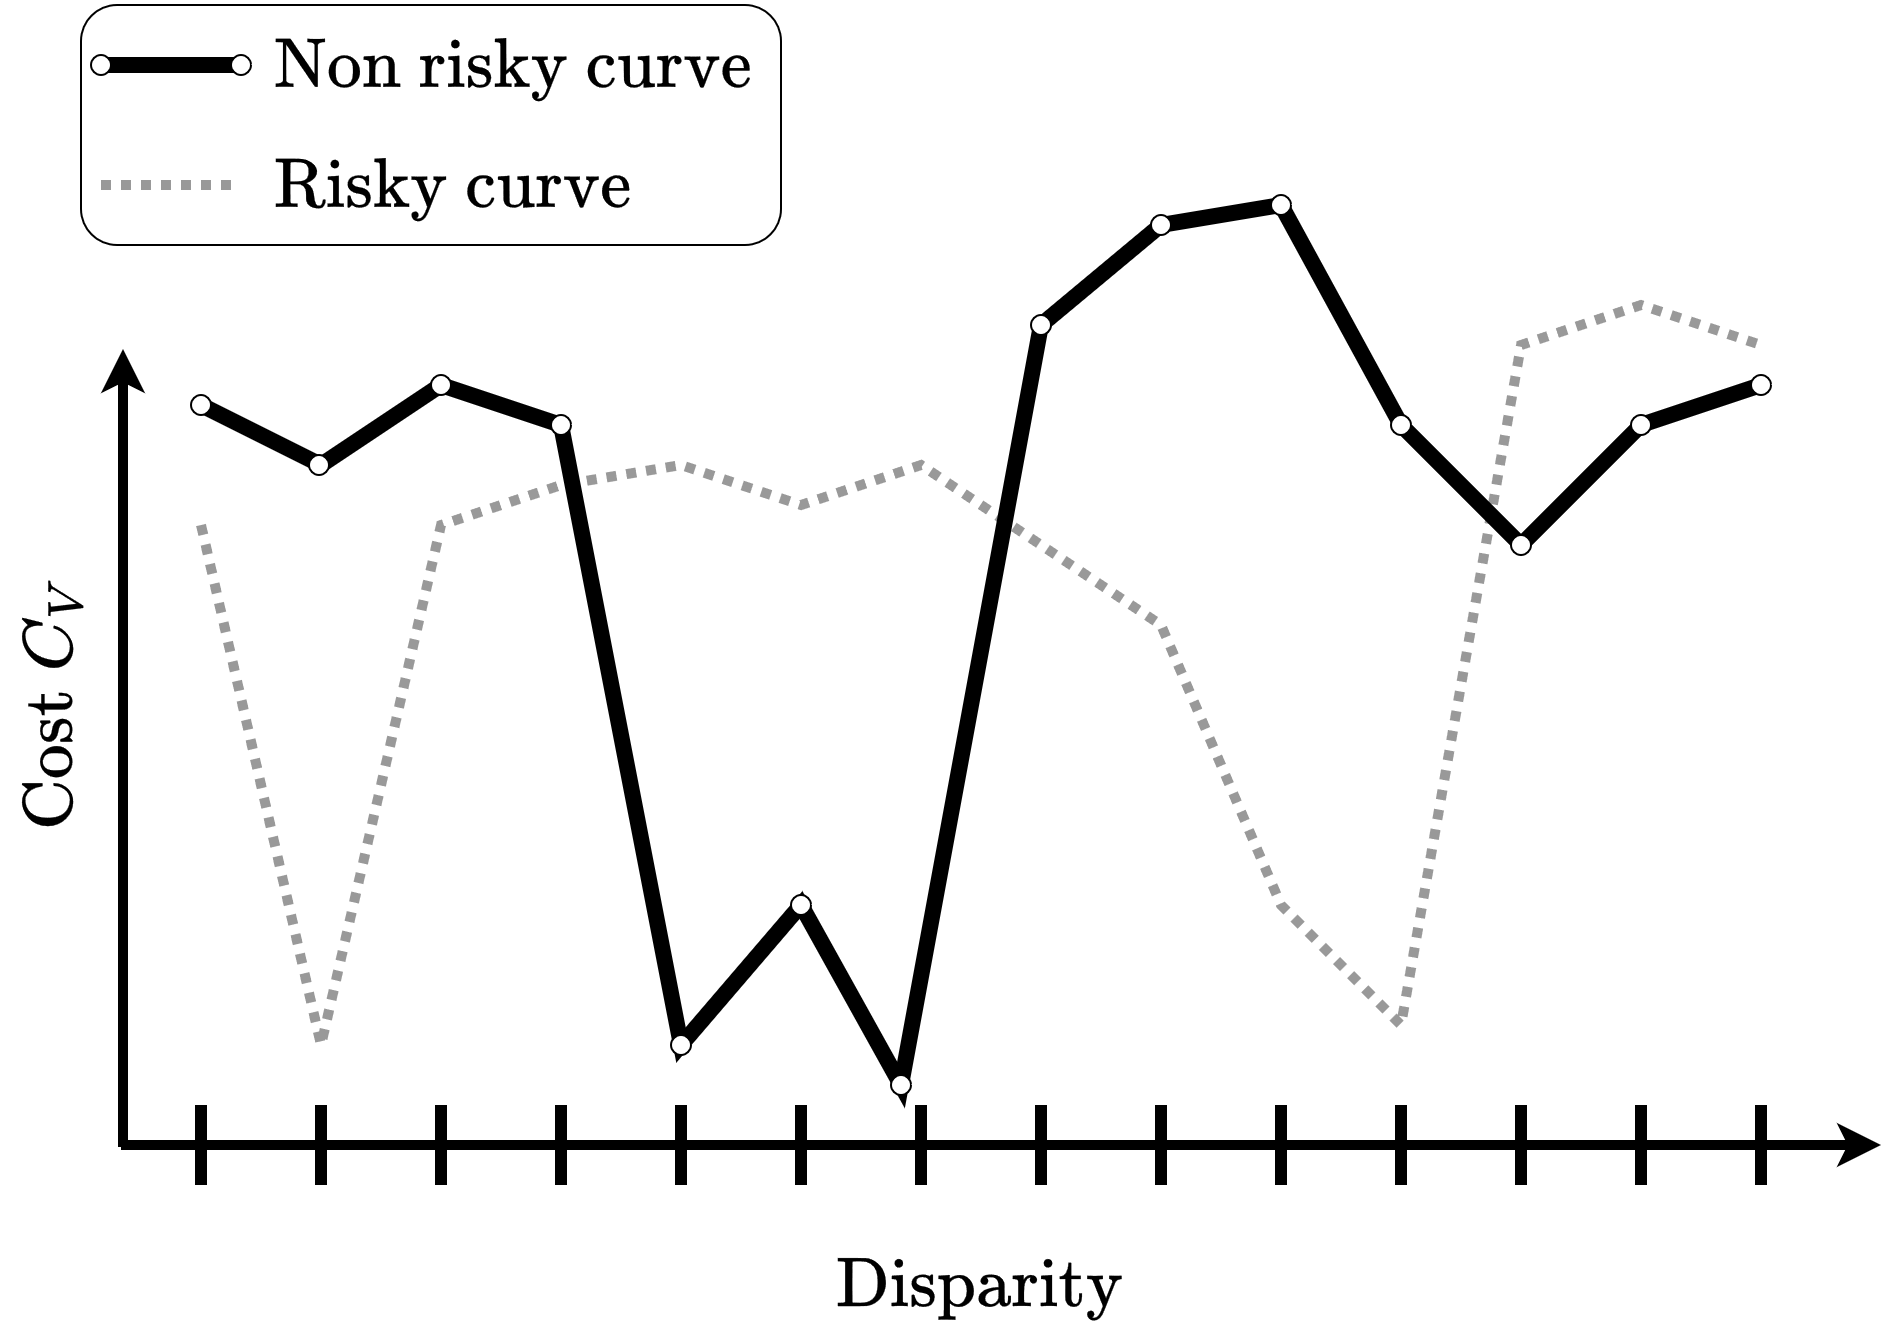
\includegraphics[width=\linewidth]{Images/Chap_1/Risk.png}
        \caption{}
        \label{fig:risk}
    \end{subfigure}\hfill
    \caption{Cost curves with different levels of ambiguity \ref{fig:ambgiuity} and risk \ref{fig:risk}}
    \label{fig:ambiguity_risk}
\end{figure}

The first confidence measure is a confidence measure called \textit{confidence from ambiguity} \cite{sarrazin_ambiguity_2021}. This method is based on the cost volume and quantifies how easy or hard it is to single out the correct disparity in a cost curve. \Cref{fig:ambgiuity} presents two curves: one that is ambiguous and one that is not\commanue{Alors tu as une phrase qui reprend cette info en la complétant donc cette phrase est en trop.}. To compute it, we first start by constructing what is called an \textit{ambiguity curve}. We do that by counting how many disparities have a cost close within a threshold $\eta$ to the minimal cost, for increasing values of $\eta$. \Cref{fig:ambgiuity} presents two cost curves, one which is not ambiguous as there is a single well defined minimum, and an ambiguous cost curve which presents multiple values that are close to the minimum. Formally we need to define for a pixel $(row, ~col)$ the set of all disparities whose cost is within a range $\eta$ of the minimal cost, and then define the ambiguity curve as the cardinal of this set:
\begin{align}
    &\mathcal{D}_\eta = \{d ~|~ C_V(row,~col,~d) \leqslant \min_\delta C_V(row, ~col, ~\delta) + \eta\}\\
    &Amb(row, ~col, ~\eta) = \#\mathcal{D}_\eta
\end{align}
where $\#$ is the cardinal of a set. Evaluating $Amb$ for different $\eta$ gives the ambiguity curve. \Cref{fig:integral_ambiguity_1} presents a cost curve with different values of $\eta$. \Cref{fig:integral_ambiguity_2} presents the resulting ambiguity curve. On those two figures we can see for instance that for $\eta_3$ there are $6$ disparities whose cost is lower than $\min_\delta C_V(row, ~col, ~\delta) + \eta_3$. For non-ambiguous cost curves, $Amb$ will increase only for high values of $\eta$. On the contrary, for ambiguous curves, $Amb$ will be high for small values of $\eta$. To obtain a scalar value from $Amb$, we compute the area under its curve, normalized by the range of $\eta$:
\begin{equation}
    \mathrm{AUC}_{Amb}(row, ~col) = \frac{1}{\max\eta-\min\eta}\int_\eta Amb(row,~col,~\eta)d\eta
\end{equation}
However, this results on low values for confident (non-ambiguous) cost curves, and high values for less confident (ambiguous) curves. The confidence from ambiguity $c_{Amb}$ is thus obtained by normalizing and reverting the integral:
\begin{equation}\label{eq:confidence_from_ambiguity}
    c_{Amb}(row, ~col) = \frac{\max \mathrm{AUC}_{Amb}- \mathrm{AUC}_{Amb}(row, ~col)}{\max \mathrm{AUC}_{Amb} -\min \mathrm{AUC}_{Amb}}
\end{equation}
This way, values of $c_{Amb}$ near $0$ indicate that we are not confident in the predicted disparity. Reversely, values of $c_{Amb}$ near $1$ indicate that we are confident in the predicted disparity.

\begin{figure}
    \centering
    \begin{subfigure}[t]{0.6\linewidth}
        \centering
        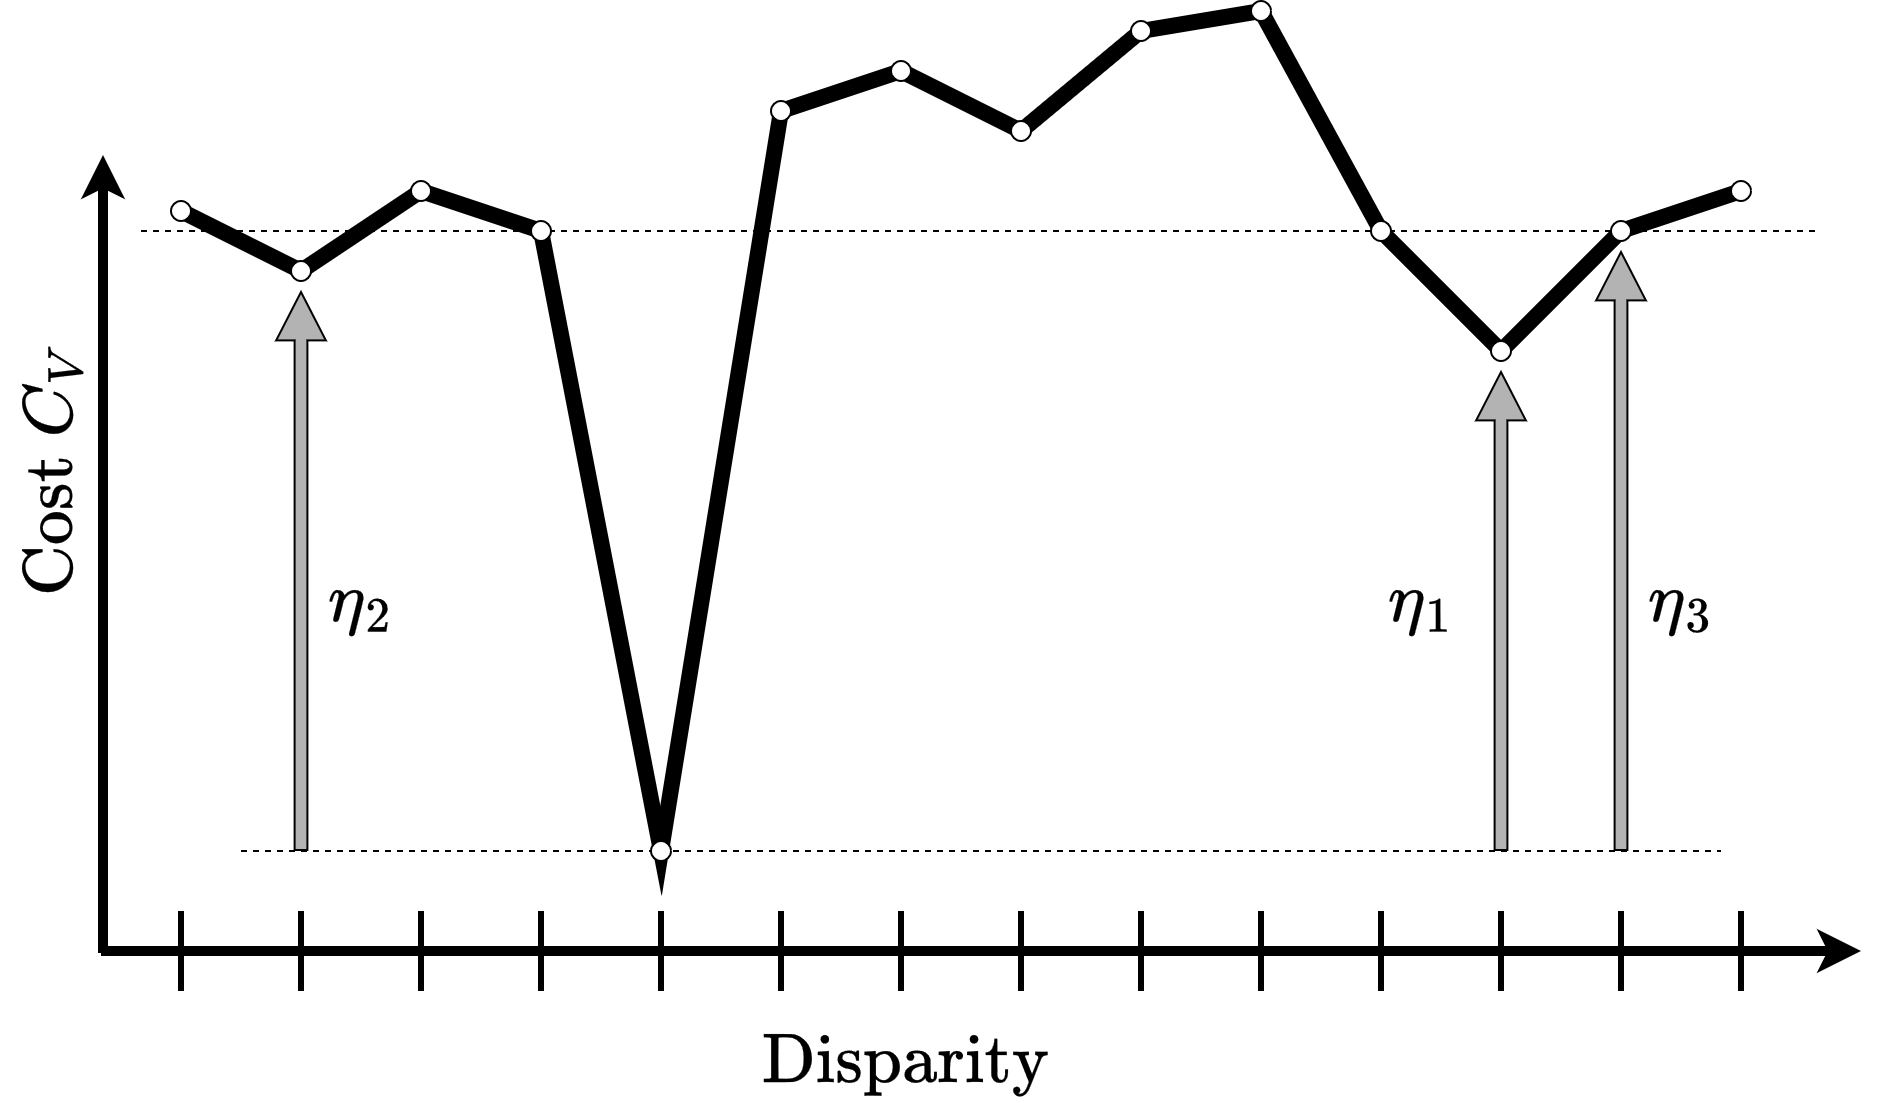
\includegraphics[width=\linewidth]{Images/Chap_1/Integral_Ambiguity_1.png}
        \caption{Cost curve with different values of $\eta$. Horizontal dotted lines indicates the range of costs between $\min_\delta C_V(row, ~col, ~\delta)$ and $\min_\delta C_V(row, ~col, ~\delta)+\eta_3$}
        \label{fig:integral_ambiguity_1}
    \end{subfigure}\hfill
    \begin{subfigure}[t]{0.4\linewidth}
        \centering
        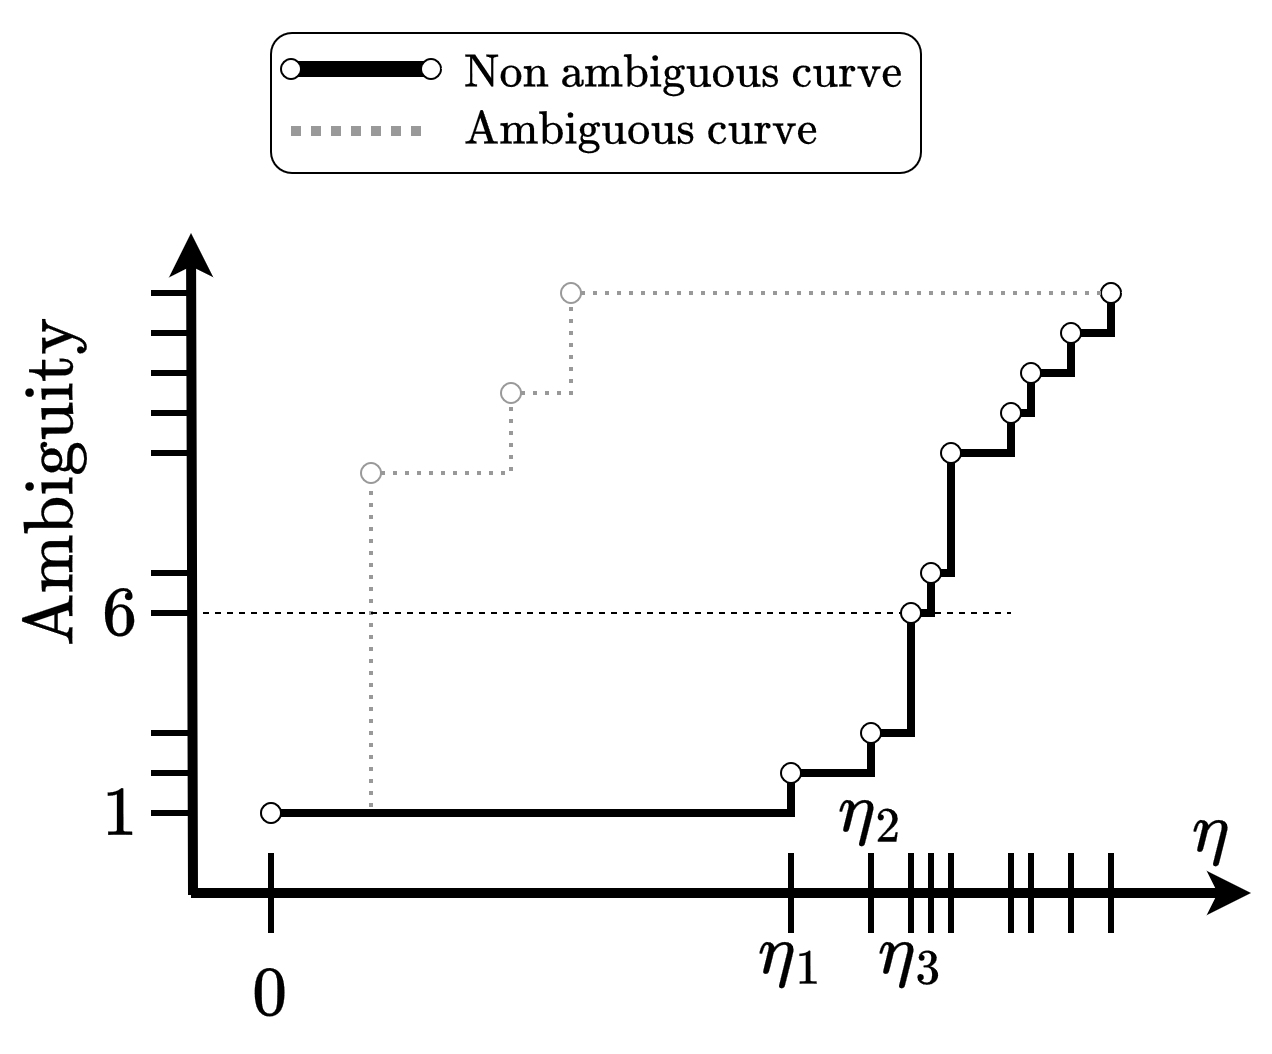
\includegraphics[width=\linewidth]{Images/Chap_1/Integral_Ambiguity_2.png}
        \caption{Associated ambiguity curve in full line. Ambiguous curve in gray dotted line}
        \label{fig:integral_ambiguity_2}
    \end{subfigure}\hfill
    \caption{Illustration of the computation of the ambiguity curve.}
    \label{fig:integral_ambiguity}
\end{figure}

The second confidence measure that we consider is named \textit{confidence from risk}. It is designed to measure if the magnitude of a potential error is high or low. After all, if we predict a wrong disparity while the correct disparity is right next to our prediction, the impact on the final result will be smaller than if the true disparity is at the other side of the disparity range. Keeping this in mind, we apply the same methodology as for the ambiguity. We consider the set $\mathcal{D}_\eta$ of all disparities whose cost is less than $\eta$ away from the minimal cost, and define the risk as the gap between extrema of this set:
\begin{equation}
    R(row, ~col, ~\eta) = \max_{\mathcal{D}_\eta}d - \min_{\mathcal{D}_\eta}d
\end{equation}
\Cref{fig:integral_risk_1} presents a cost curve with different values of $\eta$ and their associated risk $R$. \Cref{fig:integral_risk_2} presents the resulting risk for all $\eta$. For non-risky cost curves, $R$ will increase only for high values of $\eta$. On the contrary, for risky curves, $R$ will be high for small values of $\eta$. To obtain a single scalar, we compute the area under the risk curve, normalized by the range of $\eta$:
\begin{equation}
    \mathrm{AUC}_R = \frac{1}{\max\eta-\min\eta}\int_\eta R(row,~col,~\eta)d\eta
\end{equation}
$\mathrm{AUC}_R$ is thus expressed in number of disparities. Contrary to the confidence from ambiguity, the risk is kept as such with its current unity. 

\begin{remark}
     The risk measures the magnitude of the potential error, but not its probability. It is therefore possible to have a very risky cost curve, but which is not ambiguous at all. In other words, it means that the probability of an error occurring can be very low, but if it somehow happened, then the magnitude of this error would also be very low. The risk is thus a confidence measure that need to be completed by a measure such as ambiguity. On it own, it has less meaning than other measures.
     
    \begin{comment}
        As detailed in \Cref{sec:co3d}, one of the requirements of the CO3D mission is to produce a performance map associated with the output DSM, expressed in meters. In order to produce such a performance map, one of the leads explored at CNES was to combine the confidence from ambiguity and the risk. This is done by weighting the risk with $1-c_{Amb}$, so as to reduce the risk of confident pixels. The result, expressed in number of disparities, can itself be converted into meters using the disparity to altitude ratio $d_{alt}$ computed along epipolar grids (see \Cref{sec:epipolar_geometry}). Finally, internal studies using real data have concluded that a good candidate for a performance criterion was:
        \begin{equation}
            perf(row, ~col) = \min(1, ~\frac{1-c_{amb}(row,~col)}{\tau_{amb}})\cdot \mathrm{AUC}_R(row,~col) \cdot d_{alt}
        \end{equation}
        where $\tau_{amb}$ is a threshold usually set to $0.4$. In plain words, if the confidence from ambiguity drops below $1-\tau_{amb}$, then we do not use the ambiguity weighting and the performance equals $\mathrm{AUC}_R \cdot d_{alt}$. This performance criterion thus provide a confidence measure expressed in meters, associated to a 3D point, which can then be rasterized alongside the DSM to produce the desired performance map. We will use it as a comparison for our method in \Cref{chap:epistemic_uncertainty}.
    \end{comment}
\end{remark}

\todoroman{Dire qu'il y a eu des tentatives internes pour allier risk et amb pour faire une carte de perf. Nos travaux s'inscrivent dans cette continuité pour proposer une autre méthode. Il est envisagé de peut être l'utiliser dans la chaine CO3D.}

\begin{figure}
    \centering
    \begin{subfigure}[t]{0.6\linewidth}
        \centering
        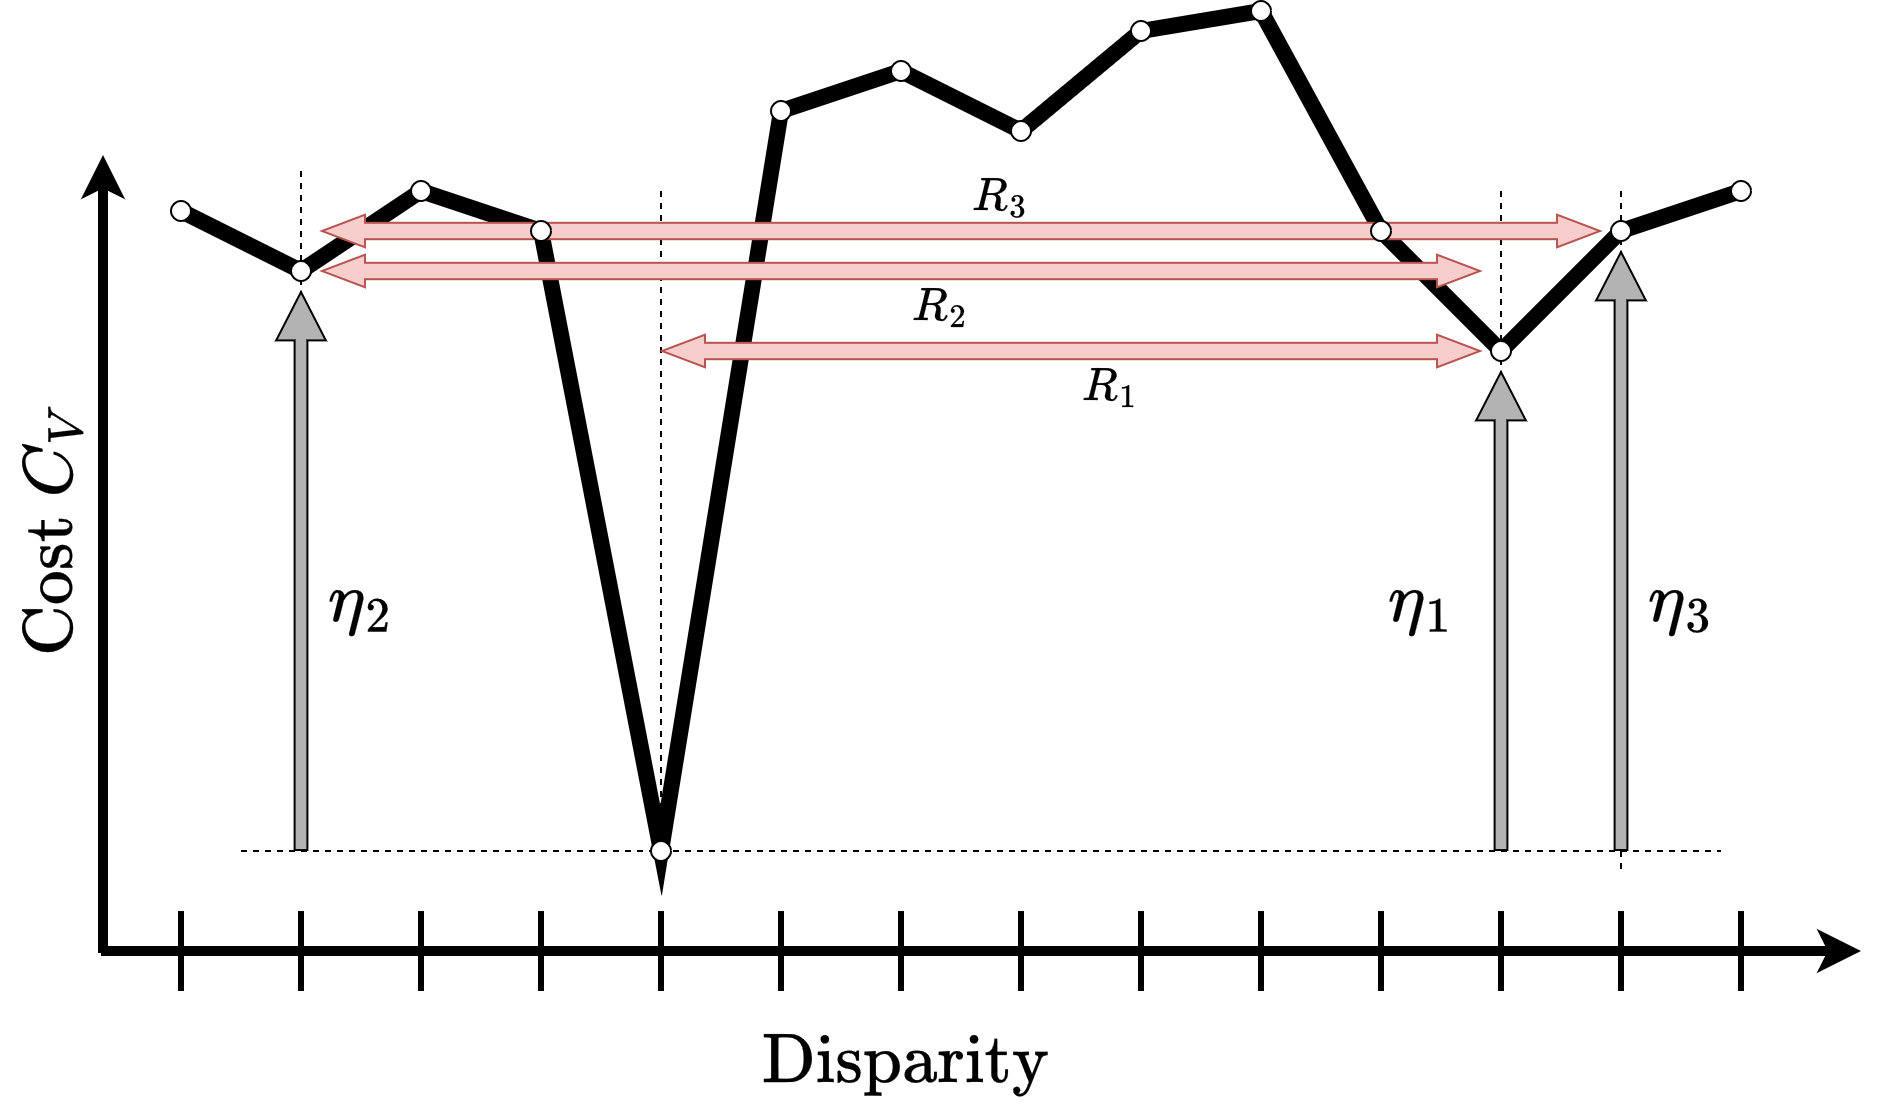
\includegraphics[width=\linewidth]{Images/Chap_1/Integral_Risk_1.png}
        \caption{Cost curve with different values of $\eta$ and risk}
        \label{fig:integral_risk_1}
    \end{subfigure}\hfill
    \begin{subfigure}[t]{0.4\linewidth}
        \centering
        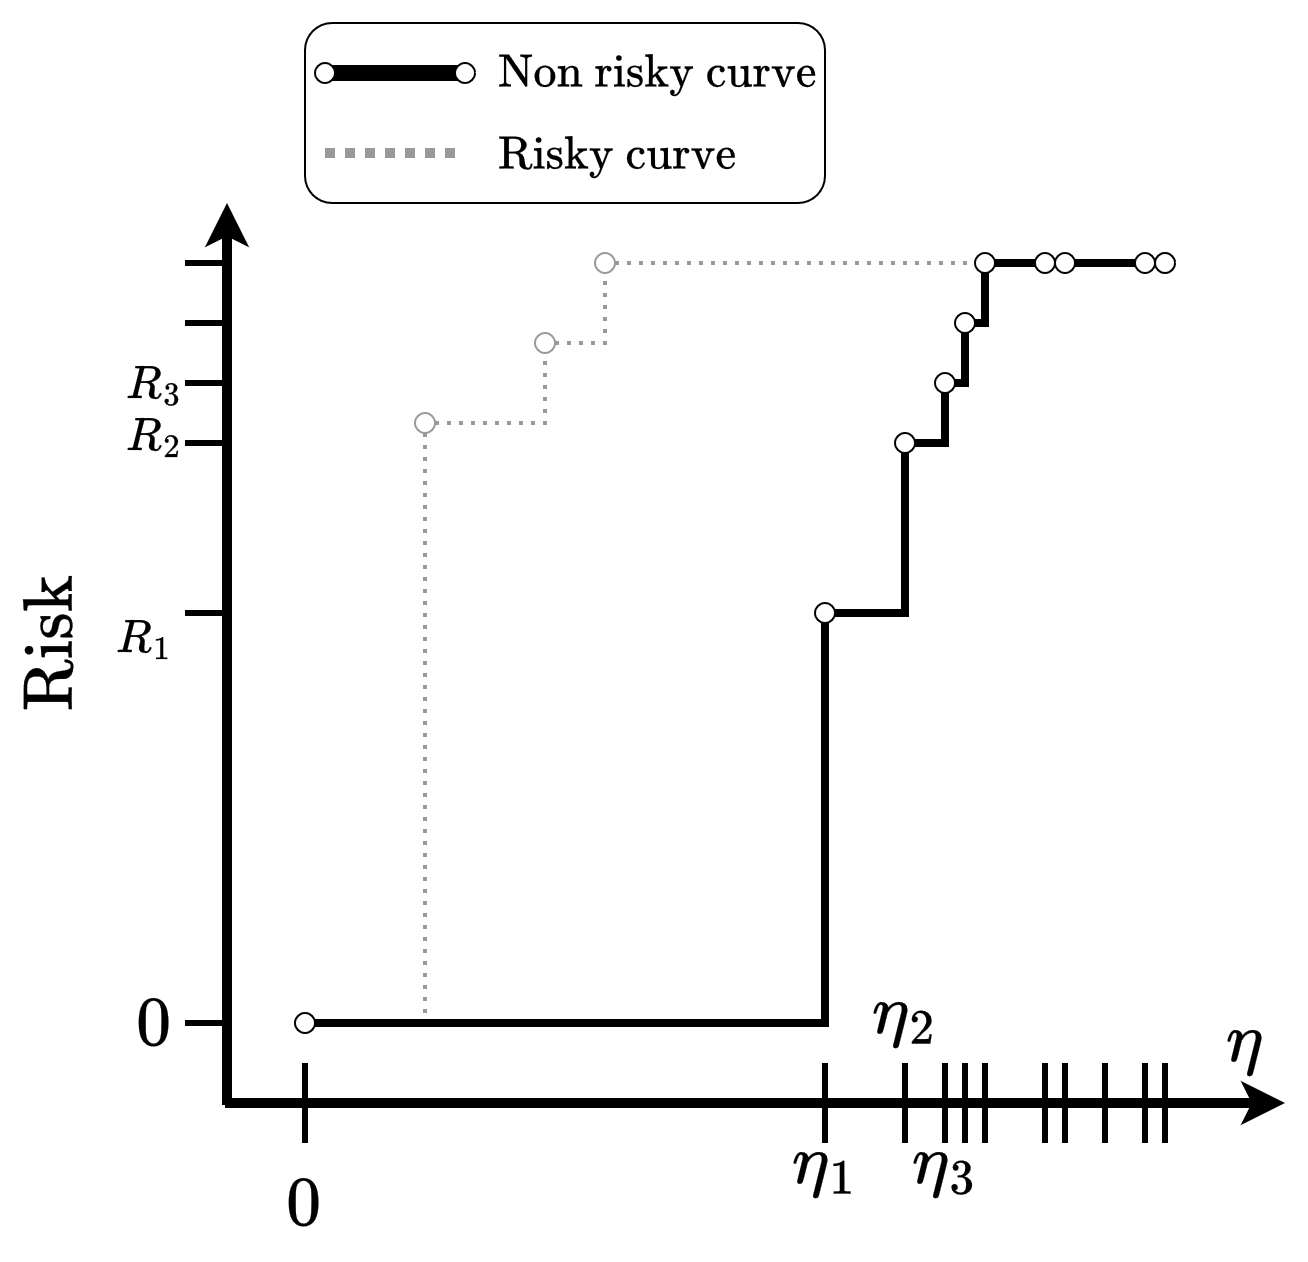
\includegraphics[width=\linewidth]{Images/Chap_1/Integral_Risk_2.png}
        \caption{Associated risk curve in full line. Risky curve in gray dotted line}
        \label{fig:integral_risk_2}
    \end{subfigure}\hfill
    \caption{Illustration of the computation of the risk curve.}
    \label{fig:integral_risk}
\end{figure}

\commanue{pas de conclusion ? en même temps tu reste constant avec tes principes}
\pagebreak
\blankpage


\chapter{Mathematical Representations of Uncertainty}\label{chap:representation_of_uncertainty}

\section{Introduction}
This chapter takes some distance from the stereo vision problem presented previously, and instead describe more formally different representations of uncertainty and the tools that can be used to manipulate them. In this thesis, we consider classical probabilities (\Cref{sec:probabilities}), possibility distributions (\Cref{sec:possibilities}) and p-boxes (secction \ref{sec:pboxes}) to model uncertainty. We also consider the case where we consider multiple sources of uncertainty simultaneously. In this setting, the dependency between the different sources must be taken into account. We thus present a dependency model called copulas in \Cref{sec:copulas}, and some of its properties. The thorough presentation of those concepts will then be put into relations in \Cref{chap:joining_credal_sets}. 

\section{Notations}
We introduce here a few notations that will be used in the rest of this chapter. \todoroman{A ajouter au fur et à mesure, peut être déplacer au début de la thèse, à côté du glossaire.} \commanu{en effet, pas mal à coté du glossaire, mais garder une phrase avec un lien pour aller les chercher si besoin pour le lecteur. sinon pas sur de l'anglais pour 'the rest of this chapter', ca sonne très francais, j'enleverais. Plus simple: I (ou we mais idem pareil) introduce here... will be used in this chapter. }
\begin{itemize}
    \item \st means ``such that''
    \item We will often present theorems or results with $n$ different variables, spaces, or Cartesian products of $n$ elements. Notations therefore quickly become quite heavy. We try our best to make them clear and readable, which is why we often use the contraction ``$\dots$'' to imply that we are enumerating all variables\commanu{.tu peux simplifier cet item qui sonne lourd. Genre ... become quite heavy. for that reason, We often use the contraction... et peut etre possible de le simplifier plus à l'essentiel}. For instance, if we apply a function $f$ to four variables $x_1, x_2, x_3, x_4$, we will write $f(x_1\enum x_4)$.
    \item When working with $n$ variables, the index $i$ will usually be used to refer to the $i$-th variable (or one of its attribute), and will be appended as a subscript when possible, otherwise as a superscript. For instance, if $x\in\mathbb{R}^n$, then $x_i$ will refer to the $i$-th component of $x$. If $m_\times\in\mathbb{R}^n$, then $m_\times^i$ will refer to $i$-th component of $m_\times$.
    \item $\opi\cdot,\cdot\cli$ refers to an interval of integers. For instance $\opi1,~4\cli=\{1,~2,~3,~4\}$. 
    \item CDF will refer to Cumulative Distribution Function\commanue{Tu n'as pas une section acronymes?}, \ie if $X$ is random variable in $\mathbb{R}$ and $P$ its associated probability, then the CDF of $X$ is $F(x)=P(X\leqslant x)$.
    \item The power set of a set $\X$ is noted $2^\X$. It corresponds to the set of all sets included in $\X$. In the discrete case, if the cardinal of $\X$ is $n$, then the cardinal of the power set is $2^n$, thus the notation.
\end{itemize}

\section{Different Models to Represent Uncertainty}\label{sec:different_models_of_uncertainty}
Assessing the reliability of an engineering system requires to quantify the uncertainty of the input parameters or of the system itself, using models of uncertainty. Modelling the uncertainty can be done in various ways, depending on the type of uncertainty considered and the available measures or \textit{a priori} regarding the uncertain sources. Most common models are probability distributions, which have been studied extensively. When using those models, we know -or suppose- that the information we try to estimate is of stochastic (or random) nature, and that we are able to precisely describe its structure using a probability distribution. However, there are many cases where such assumptions cannot be made: for instance when data is insufficient to determine the correct probability distribution, or when the uncertainty is not random but epistemic. In those cases, we can use other models such as\commanue{Ce serait top de prendre le même exemple et de montrer comment l'incertitude est modélisé différemment, si c'est possible}\comloic{ouais dans un encas "exemple" ;-)}:
\begin{itemize}
    \item fuzzy sets \cite{zadeh_fuzzy_1999} when trying to estimate the degree of truth of a statement such as ``This person is tall''
    \item intervals \cite{jaulin_applied_2001}, where no preferences are given inside a specific range of possible values
    \item imprecise probabilities which tries to extend the concept of probabilities in order to model epistemic uncertainty \commanu{ref ?}
\end{itemize}
This list is not exhaustive. Additionally, those different models can sometimes be equivalent. Choosing to use one or another depends on the nature of the problem and of the available data. In this chapter, we will mainly consider probability distributions (\Cref{sec:probabilities}) and imprecise probabilities (\Cref{sec:imprecise_probabilities}). Two specific cases of imprecise probabilities will be detailed, namely possibility distributions in \Cref{sec:possibilities} and p-boxes in \Cref{sec:pboxes}.

\begin{remark}
    Distinguishing between stochastic and epistemic uncertainty is a model accepted by many to distinguish between different situations of uncertainty. One could argue that stochastic uncertainty is, to a certain degree, the same thing as epistemic uncertainty. Indeed, if we had enough knowledge on initial conditions of a dice throw for instance (force and torque applied on the dice, its exact shape and mass distribution \etc), as well as the exact physics model, one could predict with certainty on which side it would land. There would therefore be no aleatoric process at stake here. The question of whether or not we should make the distinction between aleatoric and epistemic uncertainty is of interest regarding theoretical aspects of the nature of uncertainty. For real-life applications however, differentiating between the two seems reasonable as we cannot know every parameter and exact model at stake for every quantity of interest. 
\end{remark}

At the end of the day\comloic{et au début du suivant ? sachant que la nuit porte conseil ;-) désolé j'aime bien cette expression d'américain elle me fait toujours sourire}, choosing one model over another is not always straightforward. It requires to be aware of the type of uncertainty faced, of the strengths and limitations of each model, of the tools available to manipulate the models \etc When it comes to less common models cited above, it fundamentally requires to be aware of the existence of such models, which is not always the case for non-specialists\comloic{merci}. During this thesis, we tried to promote less common models\comloic{oui je l'ai senti comme ça aussi :-)}, especially possibility distributions \commanu{, knowing that research is made also by finding new possibilities by confronting research fields ... est ce que tu dis quelque part que c'est un des premiers travail qui mélange proba imprécise et 3D/téledection? c'est quand meme à noter ! }. We did so by presenting real life cases where they could be used while improving uncertainty modeling in the field of stereophotogrammetry (see chapters \ref{chap:propagating} and \ref{chap:epistemic_uncertainty}). \comroman{Je pense que cette remarque devrait plutôt se retrouver dans l'intro de la thèse, car elle s'éloigne de ce qui suit. Peut être même que les deux paragraphes pourraient être déplacés dans l'intro}\commanue{Oui tu peux mettre cela dans l'intro, ce sera mieux. Après la remarque est très bien}

\subsection{Probabilities}\label{sec:probabilities}
Probability measures are a classical framework to represent uncertainty. There are multiple ways of interpreting them, mainly with a \textit{frequentist} approach, or a \textit{Bayesian} approach. From a frequentist point of view, probabilities are well fitted to represent stochastic uncertainty, \ie uncertainty regarding events that can get a different result each time we run an experiment or acquire a measure (typically, noise on a sensor). From a \textit{Bayesian} point of view, probabilities represent a state of knowledge or degree of belief, and can be updated with additional information. This leads to the notion of prior and posterior probability that will not be considered in this thesis.

We remind here basic definitions regarding probability distributions.
\begin{definition}[Probability Space]\label{def:probability_space}
    We call a probability space $(\X,~\mathcal{A},~P)$ a tuple where:
    \begin{itemize}
        \item $\X$ is the set of possible outcomes (for instance head or tails for a toss coin), also called frame of discernment.
        \item $\mathcal{A}$ is the set of all subsets of $\X$ for which a probability can be measured (for instance $\{\emptyset, \{\text{heads}\}, \{\text{tails}\}, \{\text{heads, tails}\}\}$)
        \item $P$ is the probability measure assigning a probability to each of the sets of $\mathcal{A}$. For instance for a fair coin, $P(\emptyset)=0$, $P(\{\text{heads}\})=P(\{\text{tails}\}=0.5$ and $P(\X)=1$.
    \end{itemize}
    Note that $\mathcal{A}$ must be a $\sigma$-algebra meaning that it is closed under complement, countable unions and countable intersections. $P$ is a probability measure if it verifies all the Kolmogorov axioms:
    \begin{itemize}
        \item $\forall A\in\mathcal{A},~P(A)\in[0,1]$
        \item $P(\X) = 1$
        \item for any countable disjoint family of sets $A_i\in\mathcal{A}$, $P(\cup_i A_i)=\sum_i~P(A_i)$
    \end{itemize}
\end{definition}

\begin{definition}[Random Variable]
    A random variable $X$ is a measurable function from $\X$ to a measurable space (which is often $\mathbb{R}$ or a subset of $\mathbb{R}$). We can then measure the probability that $X$ takes a value in $E\subseteq\mathbb{R}$\commanue{Pourquoi E est inclus dans R. Ton sous-ensemble E ne devrait pas inclus dans un espace mesurable noté la lettre que tu veux}:
    \begin{align*}
        P(E) = P(\{x\in\X~|~X(x)\in E\})
    \end{align*}
\end{definition}

Using a random variable allows to consider the probability measure on different spaces. We then call $P$ the probability distribution of the considered random variable $X$.

Other useful concepts regarding probability distributions are cumulative distribution functions and density functions \commanu{on dit souvent CDF et PDF probability density function, utile comme acronyme après ?}:
\begin{definition}[Cumulative Distribution Function]\label{def:cdf}
    A Cumulative Distribution Function $F_X$ of a random variable $X$ with real values is the probability that $X$ will be less or equal to a number $x$. Formally, we define $F_X:\X\rightarrow[0,1]$:
    \begin{equation*}
        \forall x\in\X,~F_X(x)=P(X\leqslant x)
    \end{equation*}
\end{definition}

\begin{definition}[Density Function]\label{def:density}
    A random variable $X$ is said to possess a density function if there exists a positive integrable function $f$ over $\mathbb{R}$ \st $\forall (x_1, x_2)\in\mathbb{R}^2$:
    \begin{equation*}
        P(x_1\leqslant X \leqslant x_2) = \int_{x_1}^{x_2}f(x)dx
    \end{equation*}
    In the discrete case, the density is also called \textit{probability mass function}, and is defined as \commanue{Alors wikipedia me donne un signe $=$ et pas $\leqslant$ mais je regarde peut-être pas le bon truc}:
    \begin{equation*}
        f(x_1) = P(X \leqslant x_1)
    \end{equation*}
    In the continuous case, the density $f$ is also the derivative of the CDF of $X$\commanue{Je mettrais la remarque avant la partie discrète}.
\end{definition}
%For instance, the uniform distribution on the interval $[1,100]$ has a density function $f(x)=\frac{1}{100-1}$ if $x\in[1,100]$ and $0$ elsewhere. Its CDF is thus $0$ if $x<1$, $\frac{x}{100-1}$ if $x\in[1,100]$ and $1$ elsewhere. The concept of a CDF for multiple variables will be explored in \Cref{sec:copulas}.

In the rest of the chapter, we consider random variables $X$ on discrete spaces $\X$. If $\X=\{x_1,~\dots,~x_n\}$, we call $\{x_i\}$ an atom of $\X$, and the probability distribution $P$ of $X$ on $\X$ is completely determined by its density, which is the value of $P$ on atoms. For simplicity of notation, we will not always use braces around atoms when computing their probability. So we will sometimes write $P(x_1)$ instead of $P(X=\{x_1\})$.

As stated previously, probability measures are fitted to represent stochastic uncertainty. The following example illustrates why probability measures are not adapted to represent epistemic uncertainty:
%%%% Complex example, a simpler one is presented bellow
%\begin{example}
%    Consider a thermometer measuring the temperature of an unknown container. We only know that the temperature is above $1$ and bellow $100$ degrees Celsius. We define $X:\X\rightarrow[1,~100]$ as the random variable representing the output of the thermometer and are interested in its value. In the absence of further information on the container, a common procedure is to associate the uniform distribution to $X$. The CDF $F_X$ of $X$ is thus:
%    \begin{equation*}
%        \forall x\in\mathbb{R},~CDF_X(x)=\mathds{1}_{[1,~100]}(x)\frac{x}{100-1}
%    \end{equation*}
%    We now consider a random variable $Y$ defined as the logarithm of $X$: $Y=\ln X$. We still do not have any further information on the device and we have thus no preference on the values of its logarithm. Following the method above, one could also be tempted to associate a uniform distribution to $Y$. However, computing the CDF $F_Y$ of $Y$ from that of $X$ yields for all $y$:
%    \begin{align*}
%        F_Y(y) &= P(Y\leqslant y) = P(\ln(X)\leqslant y) = P(X \leqslant e^y) = F_X(e^y)\\
%        &= \mathds{1}_{[1,~100]}(e^y)\frac{e^y}{100-1}
%    \end{align*}
%    Which is clearly not the CDF of a uniform distribution. This is because a uniform distribution is well suited for representing statements like ``all values have the same likelyhood'' but not for statements like ``I have no information over the values (and thus no preference)''. In general, probability distributions cannot represent epistemic uncertainty as a probability distribution actually contains a lot of information about a random variable.    
%\end{example}
\begin{example}\label{ex:proba_limitations}
    Let consider a card facing down, with a number written on its hidden side. The person who wrote the number tells you that they chose to wrote either $1$, $2$ or $3$ on it. We should not\comloic{note ? know ?} that because they chose to write a number, the uncertainty on its value is not random. They then ask you to evaluate your chances of guessing the correct number and its parity, \ie if it is odd or even. We first consider the random variable $X$ taking values in $\{1,~2,~3\}$. Because you have no further information and thus no preferences on the values of $X$, a common (yet false) decision is to associate the uniform distribution $P$ to $X$:
    \begin{equation*}
        P(X=1)=P(X=2)=P(X=3)=\frac{1}{3}
    \end{equation*}
    For the parity of the number, we may now consider the random variable $Y$ defined such that $Y=0$ if ``$X=1$ or $X=3$'' and $Y=1$ if ``$X=2$''. Because we have no information on the number written on the card, we also do not have any preferences on the values of $Y$. Following the same reasoning as before, one might be tempted to associate an uniform distribution to it. However, deducing the density of $Y$ from that of $X$ yields:
    \begin{equation*}
        P(Y=0)=P(X=1)+P(X=3)=\frac{2}{3},\qquad P(Y=1)=P(X=2) = \frac{1}{3}
    \end{equation*}
    Which is clearly not the density of an uniform distribution. By supposing we have no preferences on the values of a variable, we actually deduced preferences on the values of another variable. One should use an uniform distribution only when they are certain that all values are equiprobable. This is because uniform distributions are well suited for representing statements like ``all values have the same likelyhood''\commanu{likelihood plutot} but not for statements like ``I have no information over the values, and thus no preference''. Indeed, a probability distribution actually contains a lot of information about a random variable, which is not suited to represent epistemic uncertainty.\commanue{J'aime bien l'exemple il faudrait peut-être juste ajouter des mots de liaison pour bien distinguer les différents raisonnements entre eux.}
    
    \begin{remark}
        From a Bayesian point of view, a probability can also represent a degree of belief, allowing them to represent epistemic uncertainty and not only stochastic uncertainty, in theory. However, it does not solve the expressiveness problem raised by this example. Bayesians are still reasoning with probabilities, which make no difference between ``I have no preference between these events'' and ``these events are equiprobable''. Even though they can update their prior with additional information, this would not fix the problem presented here. In the absence of additional information, basing a decision on the prior would lead to debatable conclusions.
    \end{remark}
\end{example}

\subsection{Imprecise Probabilities}\label{sec:imprecise_probabilities}
As highlighted in example \ref{ex:proba_limitations}, uncertainty cannot always be correctly modeled by probabilities, especially in a context where data is sparse. To overcome this problem, a generalization of probabilities have been introduced, called \textit{imprecise probabilities}. Imprecise probabilities (sometimes abbreviated IP) provide a general framework for working with both aleatoric and epistemic uncertainty with the concept of lower and upper probabilities. Lower and upper probabilities are quite  generic and flexible, and can be derived in more specific models. Here is a brief scope of the relevant tools it compasses: the special case of \textit{belief functions}, themselves containing specific sub-categories such as possibility distributions \ref{sec:possibilities} and probability boxes \ref{sec:pboxes} \etc\commanue{Je mettrais pas le etc} It also contains probabilities presented in \Cref{sec:probabilities}, which we will call \textit{precise} probabilities by opposition to \textit{imprecise} probabilities. \Cref{fig:diagram_IP} sums up the relationship and specificity of each imprecise model.

\begin{remark}
    At its more generic\commanu{bizarre l'anglais, On a more generic level par exemple ?}, IP can be described by sets of acceptable gambles, and by lower and upper expectations \cite{walley_statistical_1991,augustin_introduction_2014}. Although very interesting, we did not use them in our applications and thus do not consider them in this thesis.
\end{remark}
\begin{figure}[ht]
    {\centering
    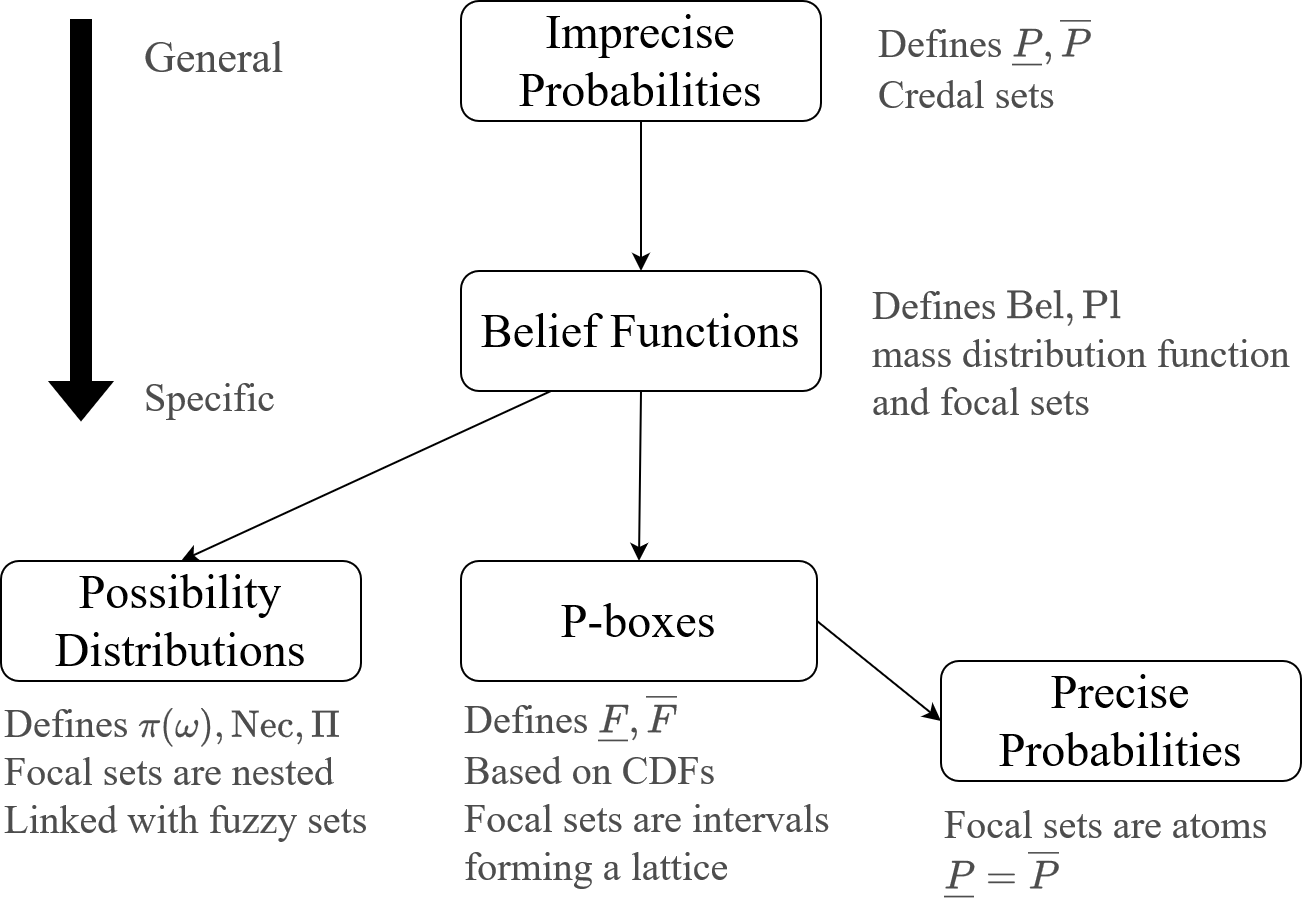
\includegraphics[width=0.8\linewidth]{Images/Chap_2/Diagramme_IP_Bel.png}
    \caption{Diagram representing the relationship between different Imprecise Probabilities models presented throughout \Cref{sec:different_models_of_uncertainty}.}
    \label{fig:diagram_IP}}
\end{figure}\commanue{La figure est bien pour voir les liens après je ne sais pas s'il faut garder les éléments en gris clair, c'est un peu déroutant pour le lecteur qui découvre les éléments}

As stated previously, a core concept of imprecise probabilities are lower and upper probabilities. Similarly to precise probabilities, a lower probability $\low$ and an upper probability $\overline{P}$ are mappings from a $\sigma$-algebra $\mathcal{A}$ to $[0, 1]$. However, while a probability $P$ gives a single measure of uncertainty for every event, lower and upper probabilities provide two bounds for every event, allowing them to express more complex uncertainty structures.

\begin{remark}
    Formally, a lower probability $\low$ needs to be \textit{super-additive}, \ie to verify:
    \begin{equation}
        \forall A,B\in\mathcal{A}, \text{ if } A\cap B\neq\emptyset, ~\low(A\cup B)\geqslant \low(A)+\low(B) \label{eq:super_additivity}
    \end{equation}
    Conversely, an upper probability is sub-additive, meaning that it verifies the same property than \cref{eq:super_additivity} but with the inequality reversed.
    
    Those properties are less constraining than their equivalent for precise probabilities in definition \ref{def:probability_space}, so lower and upper probabilities are generally \textit{not} precise probabilities. The only case where they are precise probabilities is when $\low=\overline{P}$, because $\low$ is then additive as it is both super and sub-additive. In this case, imprecise probabilities are actually a single precise probability. This illustrates the fact that precise probabilities are special cases of imprecise probabilities. 
\end{remark}

Precise probabilities define a measure of uncertainty towards a random variable $X$ taking numerical values. Imprecise probabilities however, can model the uncertainty towards a random variable taking set values instead of numerical one. We then say that $X$ is a \textit{random set} instead of a random variable. That being said, IP can also represent the uncertainty of random variables for which we suppose a precise probability exists, but we are not able to determine it precisely. Indeed, lower and upper probabilities form the bounds of a family of precise probabilities called \textit{credal set}.
\begin{definition}[Credal set]\label{def:credal_set}
    Given a lower probability $\low$ and an upper probability $\overline{P}$, a credal set $\M$ is the set of all probabilities $P$ that are greater that $\low$ and lower that $\overline{P}$:
    \begin{equation}
        \M(\low, \overline{P}) = \{P~|~\forall A\in\mathcal{A},~\low(A)~\leqslant~P(A)~\leqslant\overline{P}(A)\}
    \end{equation}
\end{definition}
We refer to $\M(\low, \overline{P})$ as $\M$ when no confusion is possible. Credal sets allow to consider multiple probabilities at once, which improves on the limited expressiveness of a single probability measure. The gap between the two bounds of a credal set reflects how imprecise is the model, in terms of epistemic uncertainty.

Conversely, we can define lower and upper bounds from a set of probabilities $\M$ as:
\begin{align*}
    \forall A\in\mathcal{A},~\low(A) =& \inf_{P\in\M}P(A)\\
    \forall A\in\mathcal{A},~\overline{P}(A) =& \sup_{P\in\M}P(A)
\end{align*}

Although, it is not required, we usually assume credal sets verify additional properties expressed as follows:
\begin{definition}[Coherence and Avoiding sure loss]\label{def:coherence_sure_loss}
    A credal set $\M$ is said to avoid sure loss if it contains at least one probability measure, \ie if
    \begin{equation}
        \M \neq \emptyset\label{eq:avoid_sure_loss}
    \end{equation}
    
    A credal set $\M$ is said to be \textit{coherent} if its lower and upper bounds on all events are attained by a probability measure, \ie if:
    \begin{equation}
        \forall A\in\mathcal{A}, \exists P, P'\in\M~\st~\low(A)=P(A) \text{ and } \overline{P}(A)=P'(A) 
    \end{equation}
\end{definition}
The bounds $\low, \overline{P}$ of a coherent credal set verifies the following property:
\begin{equation}
    \forall A\in\mathcal{A}, ~\low(A) = 1 - \overline{P}(A^c)\label{eq:lower_proba_complement}
\end{equation}
which is a generalization of the classical property for computing the complement of an event with precise probabilities. This allows us to only specify the lower bound $\low$ of a credal set to completely describe it, as its upper bound is determined by $\low$. Defining a credal set requires to specify much more constraints on the probability space that in the case of probability distributions. Indeed a lower probability must be defined on every possible event, while a precise probability can be defined by its density on possible values only (instead of possible events). In the case of a discrete space with $n$ elements, a probability is completely determined by its values on the $n$ atoms, while a lower bound is completely determined by its values on the $2^n$ considered events.


\begin{remark}
    Sampling from a credal set is not straightforward. Multiple method exists, the most intuitive consisting in sampling distributions from the credal set extreme points.
\end{remark}

\begin{remark}
    With the way we defined a credal set $\M$, it is closed and convex. This is a common way of constructing credal sets, but is not the only way. We could for instance impose that all probabilities in $\M$ belong to a family of Gaussian probabilities, which would prevent $\M$ from being convex.
\end{remark}

When constructing credal sets, it is common to possess a non convex set of probabilities $S$. In that case, we can define the convex hull of a set of probabilities $S$:
\begin{definition}[Convex Hull]\label{def:convex_hull}
    The convex hull ($CH$) of a set of probabilities $S$ is the smallest (convex) credal set containing $S$:
    \begin{equation}
        CH(S) = \{~P~|~\forall A\in\mathcal{A}, ~\inf_{P_S\in S}P_S(A)\leqslant P(A) \leqslant \sup_{P_S\in S}P_S(A)\}
    \end{equation}
\end{definition}

\begin{remark}
    The convex hull is computationally heavy to compute \commanu{redondant, juste is not computer-efficent, en tout cas pas 2 fois compute ;)}. Determining the infimum and supremum of a set of probability is not trivial as it might require to iterate through every element of $S$. It is however very useful, especially in the case where we do not know the set bounds on every event. In that case, computing the convex hull also allows us to determine the bounds on those events.
\end{remark}

\begin{example}
    Let us consider the scenario presented in example \ref{ex:proba_limitations}, and model the uncertainty with a credal set instead of a single probability distribution. Because we have no information on the value written on the card except that it is in $\{1,2,3\}$, we characterize the uncertainty by lower and upper probability $\low$, $\overline{P}$ defined as follows:
    \begin{align*}
        &\low(X=1) = \low(X=2)= \low(X=3) = 0\\
        &\overline{P}(X=1) = \overline{P}(X=2)= \overline{P}(X=3) = 1\\
        &\low(X\in\{1,2,3\}) = \overline{P}(X\in\{1,2,3\}) = 1
    \end{align*}
    We can use \cref{eq:lower_proba_complement} for computing the bounds of remaining events.
    
    Here, the credal set is the largest credal set possible as its bounds are always $0$ and $1$ for events that are not $\emptyset$ or $\{1,2,3\}$. We say that it is the vacuous credal set, as it does not encode any information. It however solves the problem of a contradicting probability when evaluating the value of the card and its parity.\commanue{J'aime bien le fait de présneter l'exemple. Après j'ai des difficultés à comprendre les deux dernières phrases.}\comloic{juste pour être sur de comprendre la dernière phrase, est ce que ça veut dire que dans le premier cas on avait une contradiction car on aurait pu vouloir d'abord fixer P(Y=pair) et P(Y=impair) et se retrouver avec P(X=1)=P(X=3)=1/4, alors que là si on commence à fixer Plower et Pupper sur X ou a Pupper(Y=impair)<=2 et Plower(Y=impair)>=0 ce qui n'est pas contradictoire avec Pupper(Y=impair)=1 et Plower(Y=impair)=0 que l'on aurait fixer dans ce mode opératoire là si on n'avait pas au préalable fixer les Pupper et Plower sur X ? }
\end{example}

\subsection{Belief Functions}\label{sec:belief_functions}
A special case of imprecise probabilities are belief functions, which we will detail in this section. First, we will introduce a key concept that goes along belief functions: mass distribution functions. We will then derive belief functions from it.

\begin{definition}[Mass distribution function]\label{def:mass_distribution_function}
    Let $\X$ be a frame of discernment\commanue{alrs X à la base c'est set of possible outcomes et là tu donnes un autre nom c'est pour la même chose ou il y a une subtilité. J'aime pas les variables qui changent surtout quand je suis pas à l'aise dans le domaine}\comloic{ah ouais +1 là t'es dur avec nous}\commanu{en effet ;)} and $2^\X$ its power set. A mass distribution function (or basic probability assignment \cite{shafer_mathematical_1976}) is a function $m:2^\X\rightarrow[0,1]$ \st:
    \begin{align}
        m(\emptyset) =& 0\label{eq:mass_emptyset}\\
        \sum_{a\subseteq\X}m(a) =& 1\label{eq:mass_whole_set}
    \end{align}
\end{definition}

There are multiple ways of interpreting $m(a)$, presented bellow\commanu{below, mais la tournure de la phrase me parait lourde:}, so as to be more familiar with $m$\commanu{pas évident de comprendre ce que tu expliques: la fonction de distribution de masse ou un sous ensemble ? est ce que cette phrase peut etre tournée sans m(a) et m et avec leur description en anglais?}:
\begin{itemize}
    \item If we consider a random set $X$, then $m(a)$ encodes the probability mass that $X$ takes $a$ as its set value.
    \item If $X$ is a random variable, then $m(a)$ encodes the available evidence that the numerical value of $X$ is \textit{exactly} in $a$, without any preferences for the values within $a$. This mean there could also be another evidence that $X$ is in $a'\subset a$, encoded with $m(a')$, and which could be either lower or higher than $m(a)$ depending on the amount of evidence available. Example \ref{ex:bicycle_pressure} illustrates this with a toy scenario. 
    \item Another interpretation of $m(a)$ is to link it to probability masses (definition \ref{def:density})\commanue{C'est bizarre de dire anaother car le premier parle déjà du lien entre m(a) et probability mass. Peut-être dire precise probability mass pour que ce soit plus clair}. If we suppose there exists an unknown underlying probability measure $P$ for $X$, $m(a)$ measures the probability mass that is assigned to $a$, but that can move freely to every point of $a$ without any preference. In other words, with more information, we could distribute $m(a)$ to every elements of $a$, and doing this for all $a$ would lead to a precise probability mass distribution.
\end{itemize}

\begin{remark}
    \Cref{eq:mass_emptyset} translates the fact than there is no evidence that the uncertain variable belongs to the empty set, \ie that it is not defined. Releasing this constraint allows to accept a certain amount of contradiction in our model.
    \Cref{eq:mass_whole_set} is a convention, which states that the total amount of evidence equals $1$. It is similar to probabilities which cannot be more than $1$. 
\end{remark}

\begin{definition}[Focal set]\label{def:focal_set}
    Let $\X$ be a frame of discernment\commanue{Même remarque que précédemment sur X}, $2^\X$ its power set, and $m:2^\X\rightarrow[0,1]$ a mass distribution function. A set $a\subseteq\X$ is called a focal set of $m$ if and only if:
    \begin{align}
        m(a)>0\label{eq:focal_set}
    \end{align}
\end{definition}
Focal sets thus represent sets of the frame of discernment for which we have evidence. The set of all focal sets is sometimes called the \textit{core} of $m$.

\begin{definition}[Belief function, Plausibility function]\label{def:belief_plausibility}
    Let $\X$ be a frame of discernment, $2^\X$ its power set, and $m:2^\X\rightarrow[0,1]$ a mass distribution function.
    
    We define the belief function associated with $m$ as the function $\Bel:2^\X\rightarrow[0,1]$ who associates to all events $A$ in $2^\X$:
    \begin{align*}
        \Bel(A)=\sum_{a\subseteq A} m(a)
    \end{align*}
    
    We define the plausibility function associated with $m$ as the function $\Pl :2^\X\rightarrow[0,1]$ who associates to all events $A$ in $2^\X$:
    \begin{align*}
        \Pl(A)=\sum_{\substack{a\\a\cap A\neq\emptyset}} m(a)
    \end{align*}
\end{definition}
We can interpret $\Bel(A)$ as the amount of evidence that fully support $A$, and $\Pl(A)$ as the amount of evidence that is consistent (or does not contradict) with $A$.

$\Bel$ and $\Pl$ are special cases of lower and upper probabilities, and verify \eqref{eq:lower_proba_complement} as for all events $A$ it holds:
\begin{align*}
    \Bel(A)&=\sum_{a\subseteq A} m(a)\\
    &= \sum_{a\in \X} m(a) - \sum_{a\not\subseteq A} m(a)\\
    &= 1 - \sum_{\substack{a\\a\cap A^c\neq\emptyset}} m(a)\\
    &=1-\Pl(A^c)
\end{align*}

Belief functions possess interesting properties making the credal set they induce both coherent and avoiding sure loss, motivating their extensive usage.

\begin{example}[Defining mass and belief\commanue{manque plausibility} functions]\label{ex:bicycle_pressure}
    Let us imagine an experiment where you try to estimate the pressure of the tyres of your bike, but your bicycle pump only have graduation every $1$ bar. You are able to do three measurements:
    \begin{itemize}
        \item The first measure, the needle seems to be between $4$ and $5$ bar.
        \item The second measure, the needle seems to be between $4.5$ and $6$ bar.
        \item The third measure, the needle seems to be between $4.5$ and $5.5$ bar.
    \end{itemize}
    Let us say that you trust your last measurement the most, because you got used to the movement of the needle. It is now possible to model the uncertainty of your tyre pressure using available evidence encoded in $m$:\\
    \noindent
    \begin{minipage}{0.3\textwidth}
        \begin{align*}
            m([4,~5]) ~=~ 0.3
        \end{align*}
    \end{minipage}\hfill
    \begin{minipage}{0.3\textwidth}
        \begin{align*}
            m([4.5,~6]) ~=~ 0.3
        \end{align*}
    \end{minipage}\hfill
    \begin{minipage}{0.3\textwidth}
        \begin{align*}
             m([4.5,5.5]) ~=~ 0.4
        \end{align*}
    \end{minipage}\par
    Based on this, we are no\comloic{je suppose que c'est now mais le chapitre 2 me consomme pas mal de matière grise et ce matin j'ai pas un gros stock disponible} able to express our degree of belief and of plausibility for all events. For instance:
    \begin{itemize}
        \item Our degree of belief that the pressure lies in $[4, 5]$ is $\Bel([4, 5])=0.3$, that it lies in $[4, 5.5]$ is $\Bel([4, 5.5])=0.7$ and that it lies in $[4, 6]$ is $\Bel([4, 6])=1$
        \item The degree of plausibility that the pressure equals $5$ is $\Pl (5)=1$ (totally plausible), that it equals $5.5$ is $\Pl (5.5)=0.7$ and that it equals $4$ is $\Pl (4)=0.3$.
    \end{itemize}
\end{example}

\subsection{Possibility Distributions}\label{sec:possibilities}
Another convenient model of uncertainty are possibility distributions\comloic{je me suis un peu perdu dans la structure ici. J'avais noté trois façon de modéliser l'incertitude épistémique dans le 2.3.0. Dont les proba imprécises que l'on a présenté 2.3.2. Ici l'intro c'est qu'on présente un autre modèle. Est ce qu'il manque un tiret dans le 2.3.0 ? Est ce que c'est un sous modèle des proba imprécises ? Je me mélange un peu tout seul peut être. Ah j'ai retrouvé ma réponse dans le 2.3.0: 2.3.4 et 2.3.5 sont des cas spécifiques de 2.3.2. Et bein est ce qu'on peut pas indicer les titres avec un niveau inférieur pour montrer qu'on n'est pas au meme niveau que 2.3.1 (proba précises) et 2.3.2 (imprécises) mais qu'on est dans les proba imprécises ?}. We will see that they induce a particular type of belief functions, and will be used in our applications.

\begin{definition}[Possibility distribution]\label{def:possibility}
    Let $\X$ be the frame of discernment. A possibility distribution is a function $\pi: \X \rightarrow [0,1]$ satisfying:
    \begin{equation}
    	\exists x \in \X, \pi(x) = 1 \label{eq:possibility}
    \end{equation}
    The value $\pi(x)$ represents the degree of possibility of $x$, with $\pi(x) = 1$ indicating full possibility, and $\pi(x) = 0$ indicating impossibility.
\end{definition}

Another notion closely related to possibility distributions is that of \(\alpha\)-cuts:
\begin{definition}[\(\alpha\)-cut]\label{def:alpha_cut}
    Let $\pi: \X \rightarrow [0,1]$ be a possibility distribution. Given any \(\alpha\in[0,1]\), we define the \(\alpha\)-cut of \(\pi\) as:
    \begin{align}
        \alpha_\pi=\{x~|~\pi(x)\geqslant\alpha\} \label{eq:alpha_cut}   
    \end{align}
    An \(\alpha\)-cut is thus the set of all elements of $\X$ whose possibility level is more that $\alpha$.
\end{definition}

\begin{definition}[Necessity and Possibility measures]
    It has been proven in \cite{dubois_when_1992} that a possibility distribution defines a specific type of plausibility functions called \textit{possibility} function and noted \(\Pi\). It also defines a specific belief function by duality called \textit{necessity} function and noted \(\Nec\), as well as a credal set $\M(\pi)$. They are defined as:
    \begin{align}
        &\Pi(A) = \sup_{x\in A}\pi(x)\\
        &\Nec(A)=1-\sup_{x\in A^c}\pi(x)\label{eq:bel_pl}\\
        &\M(\pi) &=\{P~|~\forall A,~P(A)\leqslant \sup_{x\in A}\pi(x)\}\\
        &=\{P~|~\forall A,~P(A)\leqslant \Pi(A)\} \label{eq:credal_set_possibility}\\
        &= \{P~|~\forall A,~P(A)\geqslant \Nec(A)\}
    \end{align}
\end{definition}

\begin{example}[Defining a possibility distribution]\label{ex:bicycle_pressure_possibility}
    Let us imagine the same setting as example \ref{ex:bicycle_pressure}, where we try to estimate the pressure of the tyres of our bike, but our bicycle pump only have graduation every $1$ bar. We are able to do the following measurements:
    \begin{itemize}
        \item During the first measurement, the needle seems to be around $4$ bar.
        \item During the second measurement, the needle seems to be around $5$ bar.
        \item During the third measurement, the needle seems to be around $4.5$ bar.
    \end{itemize}
    Let us say that we trust our measurement with a precision of plus or minus $0.5$ bars. For simplicity, we also only consider pressure values that are integers or half integers. Taking into considerations all the measurements, we can define a possibility distribution $\pi$ as:
    \begin{itemize}
        \item The value of $4.5$ being the most possible, $\pi(4.5)=1$.
        \item Values between $4$ and $5$ bar being mostly possible, we can for instance fix $\pi(4)=\pi(5)=0.8$
        \item Values $3.5$ and $5.5$ are unlikely but not impossible, we can say that $\pi(3.5)=\pi(5.5)=0.3$
        \item Other values are impossible, and thus have a possibility of $0$.
    \end{itemize}
    The possibility distribution $\pi$ is represented in \Cref{fig:possibility_distribution}
    Based on this, we are no\comloic{now aussi j'imagine} able to express the degree of necessity and of\commanu{j'enleverais le 2ieme of} possibility for all events. For instance:
    \begin{itemize}
        \item The degree of necessity that the pressure lies between $4$ and $5$ bar is $\Nec([4, 5])=1-\sup_{\rho\not\in[4,5]}\pi(\rho)=0.7$
        \item The degree of necessity that the pressure lies between $3.5$ and $5.5$ bar is $\Nec([3.5,~ 5.5]) = 1-\sup_{\rho\not\in[3.5,5.5]}\pi(\rho) = 1$\comroman{Retour à la ligne avant l'équation?}, meaning that the pressure is necessarily in this range.
        \item The degree of possibility that the pressure is either $3.5$ or  $5$ is $\Pi (\{3.5,~5\})=\sup_{\rho\in\{3.5,~5\}}\pi(\rho)=0.9$ (mostly possible).
        \item \etc for every possible event.
    \end{itemize}
\end{example}

\begin{figure}[!ht]
    \centering
    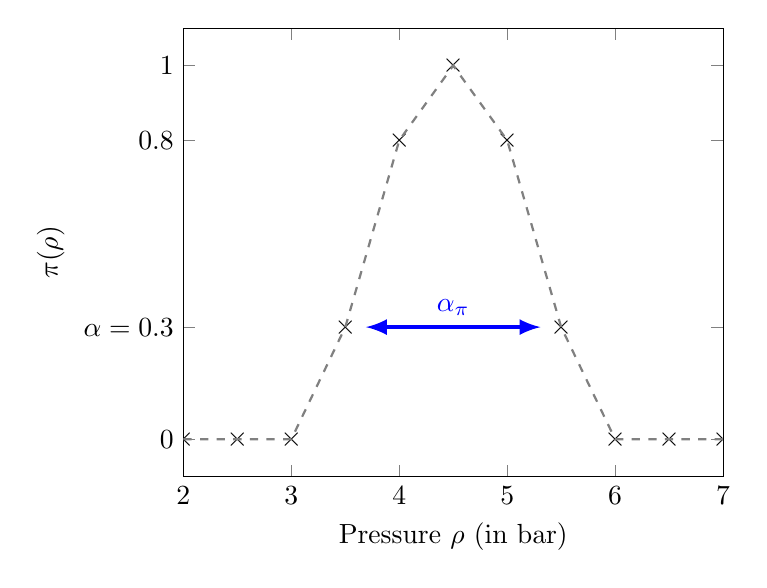
\begin{tikzpicture}[scale=1]
        \begin{axis}[%
          xlabel=Pressure $\rho$ (in bar),
          ylabel=$\pi(\rho)$,
          xmin=2, xmax=7,
          ymin=-0.1, ymax=1.1,
          ytick={0, 0.3, 0.8, 1},
          yticklabels={$0$, $\alpha=0.3$, 0.8, $1$},
          ],
          \node (a) at (2, 0) {$\times$};
          \node (b) at (2.5, 0) {$\times$};
          \node (c) at (3, 0) {$\times$};
          \node (d) at (3.5, 0.3) {$\times$};
          \node (e) at (4, 0.8) {$\times$};
          \node (f) at (4.5, 1) {$\times$};
          \node (g) at (5, 0.8) {$\times$};
          \node (h) at (5.5, 0.3) {$\times$};
          \node (i) at (6, 0) {$\times$};
          \node (j) at (6.5, 0) {$\times$};
          \node (k) at (7, 0) {$\times$};
          
          \draw [thick, dashed, gray] (a.center) -- (b.center) -- (c.center) -- (d.center) -- (e.center) -- (f.center) -- (g.center) -- (h.center) -- (i.center) -- (j.center) -- (k.center) ;
          \draw [<->, >=latex, ultra thick, blue] (d.east) -- (h.west) node [pos=0.5, above] {$\alpha_\pi$};
        \end{axis}
    \end{tikzpicture}
    \caption{Possibility distribution of example \ref{ex:bicycle_pressure_possibility} and one of its $\alpha$-cut in blue}
    \label{fig:possibility_distribution}
\end{figure}

\begin{remark}
    If you are familiar with fuzzy sets you may have noticed than\comloic{that?} possibility distributions strongly resemble\commanu{is very similar ?} to the membership function of a fuzzy set. Links between fuzzy sets and possibility measures have been explored in \cite{zadeh_fuzzy_1999}.
\end{remark}

Focal sets of necessity functions can be determined directly from the possibility distribution by looking at their \( \alpha \)-cuts. It has been proven that the core $\mathcal{C}$ (the set containing all focal sets) of a necessity function is (\cite{destercke_unifying_2008}):
\begin{align*}
    \mathcal{C} =& \{\alpha_\pi~|~\alpha\in[0,1]\}\\
    =& \{ ~\{x\in\X~|~\pi(x)\geqslant\alpha\}~|~\alpha\in[0,1]~\}
\end{align*}
With the way focal sets are defined, they form a nested family of sets with regards to inclusion. Indeed, if an element of \(\X\) belongs to an \(\alpha\)-cut, then its possibility is greater than \(\alpha\) and therefore belongs to any other \(\alpha'\)-cut with a lower \(\alpha'\). For simplicity, we will suppose that the focal sets \(a_1\enum a_n\) are already numbered using the inclusion order, \ie \( a_1\subset\dots\subset a_n\). In this case, we will refer to the inclusion order as the ``natural'' order.

\begin{remark}
    The fact that focal sets form a nested family of sets in the case of possibility distributions also implies than if $\X$ is finite and contains $n$ elements, then there can be \textit{at most} $n$ focal sets. For comparison, belief functions can have a maximum of $2^n-1$ focal sets (as the empty set cannot be a focal set). This means that necessity functions have less degrees of freedom than (some) belief functions and thus can express less uncertainty structures. This drawback comes with the advantage of being easier to construct, as we only need to specify the mass of $n$ focal sets (or the possibility of the $n$ elements of $\X$) instead of $2^n-1$. Indeed, when we think of a random variable like the outcome of a dice, it can seem more natural for someone to specify degrees of possibility for each side separately than it is to specify degrees of plausibility for different sets of outcomes. 
    
    As such, possibility distribution have been used to model experts opinion  \cite{baudrit_joint_2007}. Following the same philosophy, we will use possibility distributions in \Cref{chap:epistemic_uncertainty} to model the uncertainty of a measure of similarity between two image patches.
\end{remark}

Specifying a probability distribution often comes down to specifying the probability mass function over all atoms of the frame of discernment. In a way, possibility distributions are constructed the same way, as we specify the possibility (or the upper bounds) of every atom. One important difference is that the condition ``the sum of all masses must be equal to $1$'' is relaxed into a less constraining condition ``the possibility distribution must be equal to $1$ at least once''. In that respect, it is easier to construct a well defined possibility distribution than it is to construct a well defined probability distribution. However the comparison stops there, as the two models does not represent the same uncertainty at all.

\begin{remark}
    Any probability distribution $P$ is a belief function $\Bel$, for which focal sets are only composed of singletons (atoms) and the mass distribution function of $\Bel$ equals the probability mass function of $P$ on atoms. However, a possibility distribution cannot model a probability distribution. Indeed this would impose that its necessity $\Nec$ and plausibility $\Pi$ functions verify:
    \begin{align*}
        \forall A, &~\Nec(A) = \Pi(A)\\
        \Leftrightarrow&~1-\sup_{x\in A^c}\pi(x) = \sup_{x\in A}\pi(x)\\
        \Leftrightarrow&~ \sup_{x\in A}\pi(x) + \sup_{x\in A^c}\pi(x) = 1
    \end{align*}
    Consider this equation for any $x'$ verifying $\pi(x')=1$. This leads to the conclusion that any $x\neq x'$ has a possibility of $0$. We are in a case where it is impossible that a random set or random variable takes any other value than $x'$, which makes it not random. 
\end{remark}

\subsection{P-boxes}\label{sec:pboxes}
Another special type of belief function that is commonly used is that of \textit{probability boxes}, more commonly called p-boxes. Formally, a p-box is a pair of precise cumulative distribution functions $[\underline{F}, ~\overline{F}]$ defining lower and upper bounds on all cumulative events:

\begin{definition}[P-box]\label{def:p-box}
    Let $\X$ be the frame of discernment. A p-box is a pair of CDF $[\underline{F}, ~\overline{F}]$ from $\X$ to $[0, ~1]$ such that:
    \begin{equation}
    	\forall x \in \X,~\underline{F}(x) \leqslant \overline{F}(x) \label{eq:p-box}
    \end{equation}
    If $\X$ is not a subset of $\mathbb{R}$, then there must exists a total order on $\X$ to define a p-box. 
\end{definition}

\begin{remark}
    A probability distribution can be both determined by specifying its values on every atom or by specifying its values on cumulative events. We saw in \Cref{sec:possibilities} that possibility distributions define bounds on atoms. Because p-boxes define bounds on cumulative events, we could say that a p-box is the ``imprecise way'' of defining a probability using cumulative events, and a possibility distribution is the ``imprecise way'' of defining a probability using atoms.
\end{remark}

The credal set $\M$ induced by a p-box $[\underline{F}, ~\overline{F}]$ is:
\begin{align}
    \M([\underline{F}, ~\overline{F}]) = \{~ F ~|~ \forall x\in\X, ~\underline{F}(x)\leqslant F(x)\leqslant \overline{F}(x) ~\}
\end{align}

\begin{definition}[Focal sets of p-boxes]
    P-boxes are special cases of belief functions. It has been proven in \cite{destercke_unifying_2008} that focal sets of p-boxes have a specific form. Although focal sets shapes are reminiscent of possibilities' $\alpha$-cuts (see \Cref{fig:p-box}), they are a bit more complex to express formally. If $\X=\{x_1\enum x_n\}$ with $x_1\leqslant\dots\leqslant x_n$, then focal sets $\alpha_{[\underline{F}, ~\overline{F}]}$ of $[\underline{F}, ~\overline{F}]$ are given for every $\alpha\in[0,~1]$ by the following expression:
    \begin{align}
        \alpha_{[\underline{F}, ~\overline{F}]}= \opi \overline{F}^{-1}(\alpha),~\underline{F}^{-1}(\alpha)\cli\label{eq:pbox_focal_set}
    \end{align}
    where $\opi\cdot,~\cdot\cli$ are intervals of integers, and $\overline{F}^{-1}$, $\underline{F}^{-1}$ are the respective pseudo-inverse of $\overline{F}$ and $\underline{F}$ defined for every $\alpha\in[0,1]$ by:
    \begin{align*}
        \overline{F}^{-1}(\alpha) =& \min \{x_i ~\st ~\overline{F}(x_i)\geqslant \alpha\}\\
        \underline{F}^{-1}(\alpha) =& \min \{x_i ~\st ~\underline{F}(x_i)\geqslant \alpha\}\commanue{c'est pas un max?}\comloic{alors de ce que je comprends grace à la figure 2.3 (parce que bon avec le texte j'y étais pas non plus), c'est un max seulement si on cherche xi tel que Funder <= xi. Du coup ça a l'air ok.}
    \end{align*}
    
    Still in \cite{destercke_unifying_2008}), it has been shown that the mass of each focal set $\opi x_i, ~x_j\cli$ equals to :
    \begin{align}
        m(\opi x_i, ~x_j\cli) = \min(\overline{F}(x_i), \underline{F}(x_j)) - \max(\overline{F}(x_{i-1}), \underline{F}(x_{j-1}))
    \end{align}
    With the convention that $\max(\overline{F}(x_{i-1}), \underline{F}(x_{j-1}))=0$ if $x_{i}$ is the first element and thus $x_{i-1}$ is ill-defined. 
\end{definition}

Because of their shape, focal sets of p-boxes form a lattice on $\X$, and can be ordered. It can be easily seen by looking at \Cref{fig:p-box}. If $a$ and $b$ are two focal sets of the same p-box $[\underline{F}, ~\overline{F}]$, then they are ordered as follows:
\begin{align}
    a\leqslant b \Leftrightarrow \min(a)\leqslant\min(b) \text{ and } \max(a)\leqslant \max(b)
\end{align}
As $\underline{F}\leqslant\overline{F}$, we are assured that there can't be any case where $\min(a)<\min(b) \text{ and } \max(a)> \max(b)$\commanue{Tu t'es pas trompé de signe pour le min ?}. We can also define the order on focal sets using the definition of \cref{eq:pbox_focal_set} for every $\alpha,~\beta\in[0,1]^2$:
\begin{align*}
    \opi\overline{F}^{-1}(\alpha), ~\underline{F}^{-1}(\alpha)\cli \leqslant \opi\overline{F}^{-1}(\beta), ~\underline{F}^{-1}(\beta)\cli \Leftrightarrow \alpha\leqslant\beta
\end{align*}

Given the shape of focal sets, there can be at most $2n-1$ in a frame of discernment with $n$ elements\comloic{ça c'est un truc que j'ai encore du mal à dessiner}. This is more degree of freedom than possibility distributions, but less than general belief functions.
\begin{remark}
    Contrary to possibility distributions that cannot equal to a single probability distribution, if a p-box $[\underline{F}, ~\overline{F}]$ verifies $\underline{F}=\overline{F}$, then its credal set is composed of a single probability distribution whose CDF $F$ equals $\underline{F}$ and $\overline{F}$. P-boxes are thus generalizations of precise probability distributions.
    
    Because both $\underline{F}$ and $\overline{F}$ are precise CDF and belong to the credal set $\M([\underline{F}, ~\overline{F}])$, we already know two samples of the credal sets it defines, without having to sample from it.
\end{remark}

\begin{figure}[!ht]
    \centering
    \begin{tikzpicture}[scale=1]
        \begin{axis}[%
          xlabel=$x$,
          ylabel=$\CDF(x)$,
          %grid=major,
          domain=0:15,
          %legend entries={$\underline{F}$, $\overline{F}$},
          legend pos=south east,%
          ],
            \addplot[dotted, black, samples=16, mark=triangle, mark options={solid}, mark size=3pt] {cdf_erf(x, 1.5, 1.5)} node [pos=0.4, above left] {$\overline{F}$};
            \addlegendentry{$\overline{F}$}
            
            \addplot[dotted, black, samples=16, mark=square, mark options={solid}, mark size=3pt] {cdf_erf(x, 7.5, 1.5)} node [pos=0.6, below right] {$\underline{F}$};
            \addlegendentry{$\underline{F}$}
            
            \addplot[dotted, gray, samples=16, mark=+, mark options={solid, color=gray}, mark size=3pt] {cdf_erf(x, 4.5, 2)};
            \addlegendentry{$F$}
            
            \node (a) at (4, {cdf_erf(4, 1.5, 1.5)}) {};
            \node (b) at (10, {cdf_erf(10, 7.5, 1.5)}) {};
            
            \draw [<->, >=latex, ultra thick, blue] (a.east) -- (b.west) node [pos=0.5, above] {$\alpha_{[\underline{F}, ~\overline{F}]}$};
        \end{axis}
        \end{tikzpicture}
    \caption{A p-box $[\underline{F}, ~\overline{F}]$, a precise CDF $F$ in its credal set, and one of its focal elements $\alpha_{[\underline{F}, ~\overline{F}]}$ in blue}
    \label{fig:p-box}
\end{figure}


\section{Dependency Models: Copulas}\label{sec:copulas}
During previous sections, we presented different models of uncertainty that will be considered throughout this thesis. When we will aggregate and propagate multiple sources of uncertainty in chapters \ref{chap:joining_credal_sets}, \ref{chap:propagating} and \ref{chap:epistemic_uncertainty}, we will need to take into account the dependency between our uncertain sources. In this section, we will present dependency models called copulas, which are mathematical tools used to represent the dependency between multiple random variables. Copulas can represent many types of dependency, ranging from complete monotonicity to complete counter-monotonicity, including independence between variables. \Cref{sec:copula_def} will present the mathematical definition of a copula as well as practical families of copulas and how they can model different dependencies. \Cref{sec:dconvexity} will present a specific property shared by some copulas and a theoretical contribution that will \commanu{be ?}used later in sections \ref{subsec:pboxes} and \ref{subsec:multiple_models}. Finally, we present how to generate multivariate samples from a copula, which will be used in \Cref{sec:montecarlo}.

\subsection{Core Definitions and Examples}\label{sec:copula_def}
In the following, let $n\in\mathbb{N}^*$ be the number of sources of uncertainty considered (either represented by random variables or random sets). We first introduce copulas, which are mapping from $[0,1]^n\rightarrow [0,1]$ verifying a number of properties, and that can model dependencies when considering \hyperref[theorem:sklar]{Sklar's Theorem}, which will be presented in this section.

\begin{definition}
     A copula is a multivariate cumulative distribution function $C:[0,1]^{n}\rightarrow [0,1]$ whose marginals follow uniform distributions on $[0,1]$. It can be interpreted as a joint cumulative distribution of $n$ random variables. For all $i\in\opi 1,n\cli $, we will refer to $u_i\in[0,1]$ as its $i$-th variable (or marginal). A copula verifies a number of properties:
\begin{align}
    &\text{if }\exists j\in\opi 1,n\cli  \text{ \st }~u_j=0, \text{ then }C(u_1\enum u_j\enum u_n)=0\label{eq:zero_copula}\\
    &\forall i\in\opi 1,n\cli ,~C(1,1\enum1,u_i,1\enum1)=u_i\label{eq:copula_ones}\\
    &\forall (v_1\enum v_n)\in[0,1]^n \text{ \st }~\forall i\in\opi 1,n\cli ,~v_i\geqslant u_i\nonumber\\
    &\sum_{(w_1\enum w_n)\in\Pi_{i=1}^n\{u_i, v_i\}}(-1)^{|\{i~|~w_i=u_i\}|}C(w_1\enum w_n)\geqslant 0\label{eq:cop_hvolume}
\end{align}
where $\Pi_{i=1}^n$ is the Cartesian product of $n$ elements, meaning that $(w_1\enum w_n)\in\Pi_{i=1}^n\{u_i, v_i\}$ is a tuple of $n$ elements, where each element is either $u_i$ or $v_i$. Additionally, $|\{i~|~w_i=u_i\}|$ refers to the cardinal of the set $\{i~|~w_i=u_i\}$. 
\end{definition}

The first term in \cref{eq:cop_hvolume} is also called H-volume or hyper-volume. It is used to compute joint probability mass assignments in the precise case (and also in the imprecise case, see \Cref{sec:joint_mass}). In the rest of this thesis\commanu{j'aime pas trop in the rest, très french, We will now use... seulement?}, we will use the following notation to refer to the $H$-volume:
\begin{eqnarray}\label{eq:hvolume}
    &&\forall i\in\opi 1,n\cli ,~\forall~0\leqslant u_i \leqslant v_i \leqslant 1,\nonumber\\
    &&H^{v_1,\dots v_n}_{u_1\enum u_n}=\sum_{(w_1\enum w_n)\in\Pi_{i=1}^n\{u_i, v_i\}}(-1)^{|\{i~|~w_i=u_i\}|}C(w_1\enum w_n)
\end{eqnarray}

\begin{remark}
    The formula of the H-volume actually represents the probability that $n$-uniform random variables are in the hyper rectangle $[u_1,v_1]\tdt[u_n,v_n]$. However, it is difficult to see this interpretation in the general case just by looking at the formula. For simplicity, consider the two dimensional case. Using the interpretation of a copula $C$ as a CDF, we can image two random uniform variables $U_1$ and $U_2$ on $[0,1]$ for which $C$ is their CDF. We thus have for all $(u_1,u_2)\in[0,1]^2$:
    \begin{equation*}
        P(U_1\leqslant u_1, U_2\leqslant u_2) = C(u_1, u_2)
    \end{equation*}
    Let $(u_1,u_2)\in[0,1]^2$ and $(v_1,v_2)\in[0,1]^2$ \st $u_1\leqslant v_1$ and $u_2\leqslant v_2$. 
    Computing the H-volume of $C$ between $(v_1,v_2)$ and $(u_1,u_2)$, using different colors to help comprehension \commanu{understanding?}, yields:
    \begin{align}
        H^{v_1,v_2}_{u_1,u_2} =& ~C(v_1, v_2) - C(v_1, u_2) - C(u_1, v_2) + C(u_1, u_2)\nonumber\\
        =&~ \textcolor{blue}{P(U_1\leqslant v_1, ~U_2\leqslant v_2) - P(U_1\leqslant v_1, ~U_2\leqslant u_2)}\nonumber\\
        &- \textcolor{red}{P(U_1\leqslant u_1, ~U_2\leqslant v_2) + P(U_1\leqslant u_1, ~U_2\leqslant u_2)}\nonumber\\
        =&~ \textcolor{blue}{P(U_1\leqslant v_1, ~u_2 < U_2 \leqslant v_2)} - \textcolor{red}{P(U_1\leqslant u_1, ~u_2 < U_2\leqslant v_2)}\nonumber\\
        =&~ P(u_1 < U_1\leqslant v_1, ~u_2 < U_2\leqslant v_2)\label{eq:hvol_link_with_proba}
    \end{align}\comloic{alors là un grand merci parce que j'étais un peu coincé sur les notations dans l'eq (2.24), si j'avais su que tu avais préparé un exemple je m'y serais rendu direct ^^' En tout cas c'est bien plus clair comme ça, top!}
    This means that the H-volume represent the probability of the event
    \begin{equation*}
        u_1 < U_1\leqslant v_1, ~u_2 < U_2\leqslant v_2
    \end{equation*}
    or in other words, the probability that $(U_1, U_2)$ is in the hyper rectangle $[u_1,v_1]\times[u_2,v_2]$ (the intervals can be open or closed in the continuous case, the probability remains the same). Verifying this result can easily to the $n$-dimensional case can be done similarly\comloic{petit pb de formulation}. Example \ref{ex:hvolume} illustrates how the H-volume can be used to compute the discrete joint mass distribution function in the two-dimensional case. 
\end{remark}

A central theorem regarding copulas is \hyperref[theorem:sklar]{Sklar's Theorem} \cite{sklar_fonctions_1959}:
\begin{theorem}[Sklar's Theorem]\label{theorem:sklar}
    Let $F:\X_1\tdt\X_n\rightarrow[0,1]$ be a multivariate cumulative distribution function, where $\X_i\subseteq\overline{\mathbb{R}}$. The marginals $F_i$ of $F$ are defined as $\forall i\in\opi 1,n\cli , \forall x\in\X_i, F_i(x) = F( +\infty\enum  +\infty, x,  +\infty\enum +\infty)$ where $x$ is the $i$-th component of $F$. If all $F_i$ are continuous, then a unique copula $C$ exists:
    \begin{align}
        \forall (x_1\enum x_n)\in \overline{\mathbb{R}}^n, F(x_1\enum x_n)=C(F_1(x_1)\enum F_n(x_n))\label{eq:sklar_equality}
    \end{align}
    If some $F_i$ are not continuous, then $C$ is unique on the product of the ranges of all $F_i$.
    
    The reverse is also true: any copula applied to univariate cumulative distribution functions yields a multivariate cumulative distribution function whose marginals are the univariate CDFs.
\end{theorem}
\hyperref[theorem:sklar]{Sklar's Theorem} thus allow to express any multivariate CDF by means of its marginal CDFs. Conversely, we can join multiple CDF with a copula to create a multivariate CDF. A copula thus express the dependency between a multivariate CDF and its marginals.
 
\begin{remark}
    For marginals $F_i$ that are not continuous, then there can exist multiple copula $C$ verifying \cref{eq:sklar_equality}. However, if we note $F_i(\X_i)$ the image of $X_i$ through $F_i$, then there exists a unique copula $C$ on the ranges of images $F_1(\X_1)\tdt F_n(\X_n)$. The restriction of a copula \comloic{to?} a subset of $I^n$ containing $0$ and $1$ is called a sub-copula. Because we work in discrete spaces, we will mostly work with sub-copulas but the difference will be mostly transparent.
\end{remark}

Copulas are very useful to represent the dependency \comloic{je doute entre dependency et dependencies dans ce contexte} between multiple sources of uncertainty. As such, they can play a key role in uncertainty propagation problems, explored in \Cref{chap:propagating}.

\begin{example}[Usefulness of the H-Volume]\label{ex:hvolume}
    This example will illustrate how the H-volume of a copula can be used to compute the probability mass function of a multivariate probability. Let us imagine a game where a dealer throws two coins, and we are are interested in the joint result of the throws.\commanu{pas évident pour un néophyte de comprendre l'utilité du H-Volume dans ton exemple. Peut etre une phrase pour expliquer à quoi ca sert dans ton exemple du dealer, après tu pars vraiment dans l'explication technique math et on ne voit pas à quoi sert le H-Volume de façon imagée, à mon avis} We consider the two random variables $X_1$ and $X_2$ indicating the results of each throw:
    \begin{align*}
        &X_1=0\text{ if the first coin is heads, otherwise }X_1=1\\
        &X_2=0\text{ if the second coin is heads, otherwise }X_2=1
    \end{align*}
    Let $P_1$ and $P_2$ be the probability distributions of $X_1$ and $X_2$ respectively, and suppose that both heads and tails are possible outcomes for both coins. We now consider the joint probability distribution $P$ associated with the random variable $(X_1,~X_2)$, and we want to compute the probability mass distribution of $P$. We denote $F_1$, $F_2$ and $F$ the respective CDFs of $P_1$, $P_2$ and $P$. With this definition, $F_1$ and $F_2$ are the marginals of $F$, and Sklar's theorem states that there exists a copula $C$ such that $F=C(F_1,~F_2)$. 
    
    The probability mass distribution of $P$ can be computed by using the H-volume. Let us for instance start by computing $P(1,1)$. By noticing the fact that:
    \begin{equation*}
        \{x\in\X~|~X_1(x)=1\}=\{x\in\X~|~F_1(X_1(x))=F_1(1)\}
    \end{equation*}
    we can write that:
    \begin{align*}
        P(X_1 = 1, X_2=1) =& ~P(F_1(X_1)= 1, F_2(X_2) = 1)\\
        =& ~P(F_1(0) < F_1(X_1)\leqslant F_1(1), ~F_2(0) < F_2(X_2)\leqslant F_2(1))
    \end{align*}
    A common result in statistics states that random variables of the form $U_1=F_1(X_1)$ and $U_2=F_2(X_2)$ are uniform on $[0,1]$. We can thus apply the result from \cref{eq:hvol_link_with_proba}, which yields
    \begin{align*}
        P(X_1 = 1, X_2=1) =& ~P(F_1(0) < U_1 \leqslant F_1(1), ~F_2(0) < U_2 \leqslant F_2(1))\\
        =& ~H^{F_1(1),~F_2(1)}_{F_1(0),~F_2(0)}
    \end{align*}
    The probability of the atom $(1,1)$ is therefore equal to the H-volume computed between CDFs $(F_1, F_2)$ at $(1, 1)$ and at $(0,0)$. Following a similar reasoning, we can compute the probability of every atom and express them as H-volumes:
    \begin{align*}
        P(X_1=0, X_2=1) =& ~H_{0, F_2(0)}^{F_1(0), F_2(1)}\\
        P(X_1=1, X_2=0) =& ~H_{F_1(0), 0}^{F_1(1), F_2(0)}\\
        P(X_1=0, X_2=0) =& ~H_{0,0}^{F_1(0), F_2(0)}
    \end{align*}
    It is possible to generalize our observation: the probability of an atom $(x_1,~\dots,~x_n)$ is the H-volume computed between marginals CDFs $(F_1,~\dots,~F_n)$ at $(x_1,~\dots,~x_n)$ and at the marginal atoms that precedes them. If $x_1$ is the smallest number, then the marginal CDF $F_1$ before it equals $0$, \etc.
    Example \ref{ex:copulas} presents numerical applications of this example with different copulas.
\end{example}

It follows from \eqref{eq:cop_hvolume} that a copula is a component-wise increasing mapping. All copulas are actually dominating and dominated by two bounds (called lower and upper Fréchet–Hoeffding bounds):
\begin{align}
    &\forall u_i \in [0,1]^n,\nonumber\\
    &\max(0, 1-n+\sum_{i=1}^n u_i) \leqslant C(u_1\enum u_n) \leqslant \min(u_1\enum u_n)
\end{align}
The upper bound is a copula, usually called the Minimum copula $C_M$. It is used to model co-monotonic variables, \ie variables where high values occur at the same time (or similarly, where low values tend to occur simultaneously). Co-monotony implies a maximal covariance between variables.

The lower bound is a copula only in the case $n=2$, called the \L ukasiewicz copula $C_L$\commanue{Peut-être mettre la formule car tu mets celle pour plus de 2 dimensions}. It is used to model counter-monotonic variables, \ie variables with a perfect negative dependence between them. This explain why the lower bound is not a copula in dimensions higher that $2$ \commanue{Peut-être à reformuler, il existe toujours un copula qui atteint la borne inf mais aux dimensions supérieures c'est plus le même. Là on a l'impression que la borne inf ne peut pas être atteinte avec une copule}. Indeed, if $X$ has a perfect negative dependence with $Y$ and $Z$, then $Y$ and $Z$ cannot share a perfect negative dependence. However, for every $u_1\enum u_n$, there always exists a copula $C$ attaining the lower bound:
\begin{eqnarray*}
    \forall (u_1\enum u_n)\in[0,1]^n,~\exists C \text{ \st }~C(u_1\enum u_n) = \max(0, 1-n+\sum_{i=1}^n u_i)
\end{eqnarray*}
 
Independence between variables is modeled by the product copula $C_\Pi$\commanue{je mettrais des $\times$ dans la formule ou la symbole produit}:
\begin{equation*}
    C_\Pi(u_1\enum u_n)=u_1\dots u_n
\end{equation*}
which will be used later in subsection \ref{subsection:product_copula}. Graphical representations of the product copula and of the lower and upper Fréchet–Hoeffding bounds are represented in \Cref{fig:copulas}\commanue{Dans la figure c'est en dimension 2 donc c'est Product, Minimum and \L ukasiewicz copulas. En tout cas c'est ce qui est indiqué}. Example \ref{ex:copulas} presents a setting where the Product, Minimum and \L ukasiewicz copulas are used to model dependency between random variables.

\begin{example}[Different copulas for different dependencies]\label{ex:copulas}
    Let us try to illustrate how different copulas can represent different dependencies. 
    Consider the same setting as example \ref{ex:hvolume} with two coins being thrown. For the purpose of the example, suppose that the dealer throws the coins in a separate room, and comes back to tell the result. We thus never sees if he is cheating or not. He only provides us this piece of information: coins seems fair when looked at separately. We therefore have the following marginals:
    \begin{eqnarray*}
    \begin{cases}
        P_1(\text{heads}) = P_1(0) = 0.5\\
        P_1(\text{tails}) = P_1(1) = 0.5\\
    \end{cases}
    \qquad\text{ and }\qquad
    \begin{cases}
        P_2(\text{heads}) = P_2(0) = 0.5\\
        P_2(\text{tails}) = P_2(1) = 0.5
    \end{cases}
    \end{eqnarray*}
    
    \begin{itemize}
        \item Suppose that the dealer is not cheating and that the two coin throws are independent. In that case, the product copula $C_\Pi(u,v)=u\cdot v$ \commanue{perso je trouve le symbole $\times$ plus lisible} must be used to represent the independence between variables.
        Using results from the previous example, it holds that:
        \begin{align*}
            P(1,1) =& H_{F_1(1), F_2(1)}^{F_1(0), F_2(0)} = 1\cdot1 - 0.5\cdot1 - 1\cdot0.5 + 0.5\cdot0.5\\
            =& 0.25\\
            P(1,0) =& H_{F_1(0), 0}^{F_1(1), F_2(0)} = 0.25 \\
            P(0,1) =& H_{0, F_2(0)}^{F_1(0), F_2(1)} = 0.25 \\
            P(0,0) =& H_{0, 0}^{F_1(0), F_2(0)} = 0.25
        \end{align*}
        Remark that we indeed find the same results as if we directly multiplied the marginal probability mass distributions: $P(1,1) = P_1(1)\cdot P_2(1)$, \etc. We thus observe the famous result: if $P_1$ and $P_2$ are independent then $P=P_1\cdot P_2$.
        
        \item Imagine now that the dealer is not being fair, and actually forces the second throw to land on the same side as the first one (the coins will still seem fair when looked at separately). This kind of dependency is modeled by the Minimum copula $C_M(u,v)=\min(u,v)$. In this case, the joint probability is computed as follows: 
		\begin{align*}
            P(1,1) =& H_{F_1(1), F_2(1)}^{F_1(0), F_2(0)} = \min(1,1) - \min(0.5,1) - \min(1,0.5) + \min(0.5,0.5)\\
            =& 0.5\\
            P(1,0) =& H_{F_1(0), 0}^{F_1(1), F_2(0)} =\min(1,0.5) - \min(1, 0) - \min(0.5,0.5) + \min(0,0.5)\\
            =& 0\\
            P(0,1) =& H_{0, F_2(0)}^{F_1(0), F_2(1)} = 0 \\
            P(0,0) =& H_{0, 0}^{F_1(0), F_2(0)} = \min(0.5,0.5)=0.5
        \end{align*}
        The values taken by the joint probability are now completely different than in the independence case. We see that values $(0,1)$ and $(1,0)$ are indeed impossible to obtain, while $(1,1)$ and $(0,0)$ are equiprobable.
        
		\item Imagine now that the dealer is still not being fair, but this time forces the second coin to land on the first coin's opposite side. In other words, if the first coin lands on heads, then the dealer puts the second coin on tails, and inversely. Looking at marginal distributions separately will still suggests that the coins are fair. However, they appear fully counter-monotone when looked at jointly. In this case, the dependency is modeled by the \L ukasiewicz copula $C_L(u,v)=\max(0,u+v-1)$, and the joint probability equals:
		\begin{align*}
            P(1,1) =& H_{F_1(1), F_2(1)}^{F_1(0), F_2(0)} = \max(0, 1+1-1) - \max(0, 0.5+1-1)\\
            &- \max(0, 1+0.5-1) + \max(0, 0.5+0.5-1)\\
            =& 0\\
            P(1,0) =& H_{F_1(0), 0}^{F_1(1), F_2(0)} =\max(0, 1+0.5-1) - \max(0, 1+0-1)\\
            &- \max(0, 0.5+0.5-1) + \max(0, 0+0.5-1)\\
            =& 0.5\\
            P(0,1) =& H_{0, F_2(0)}^{F_1(0), F_2(1)} = 0.5 \\
            P(0,0) =& H_{0, 0}^{F_1(0), F_2(0)} = \max(0, 0.5+0.5-1)=0
        \end{align*}
        The values taken by the joint probability is now completely different than in the other cases. We see that values $(1,1)$ and $(0,0)$ are indeed impossible to obtain, while $(0,1)$ and $(1,0)$ are equiprobable.
	\end{itemize}
	Those three cases indicate how copulas can represent very different dependency structures from the same marginals. It also intuitiates\commanu{c'est anglais ? implies?} the fact that the \L ukasiewicz copula only allows values that are ``opposite'', whereas the Minimum copula only allows values that are similar. In those examples, the dependency is so important that knowing the result of one coin throw determines the result of the second, which is therefore modeled by extreme copulas, \ie the upper and lower Fréchet-Hoeffding bounds.  We will see in the following that there are other families of copula that allow less ``extreme'' dependencies.
\end{example}

To complete this overview of copulas, let us present other copulas that can be generated using a single parameter $\theta$ in the case $n=2$. Such famous families of copulas are presented in \Cref{tab:familiy_of_copula}. Those families are quite common in the literature, but this list is not exhaustive.\commanue{Peut-être ajouter une colonne où tu expliques leur intérêt}

Another important family of copulas is the family of Gaussian copulas. Each Gaussian copula is generated with a correlation matrix $R\in[-1,1]^{(n,n)}$:
\begin{align}
    C_R(u_1\enum u_n)=\Phi_R(\Phi^{-1}(u_1)\enum \Phi^{-1}(u_n))
\end{align} where $\Phi_R$ is the joint multivariate cumulative distribution function of a Gaussian variable with correlation matrix $R$, and $\Phi^{-1}$ is the inverse cumulative distribution function of a univariate Gaussian variable. We do not know an exact form for $\Phi_R$, but we can compute it by integrating its associated Gaussian probability density function:
\begin{align}
   \Phi_R&(\Phi^{-1}(u_1)\enum \Phi^{-1}(u_n)) =\nonumber\\ &\int_{-\infty}^{\Phi^{-1}(u_1)}\dots\int_{-\infty}^{\Phi^{-1}(u_n)}\frac{1}{\sqrt{(2\pi)^{n}|R|}}\exp(-\frac{1}{2}\begin{bmatrix}x_1 & \dots & x_{n}\end{bmatrix}R^{-1}\begin{bmatrix}x_1 \\ \dots \\ x_{n}\end{bmatrix})dx_1\dots dx_n
\end{align}
Where $|R|$ is the determinant of $R$. This family of copulas will be used in \Cref{sec:sources_of_uncertainty} to model the dependency between the random intensities of pixels of stereo images for instance. 
\begin{remark}
    The product copula is actually a Gaussian copula with the identity matrix $\mathbb{I}_n$ as its covariance matrix:
    \begin{align*}
        \Phi_R&(\Phi^{-1}(u_1)\enum \Phi^{-1}(u_n)) =\\ &\int_{-\infty}^{\Phi^{-1}(u_1)}\dots\int_{-\infty}^{\Phi^{-1}(u_n)}\frac{1}{\sqrt{(2\pi)^{n}|\mathbb{I}_n|}}\exp(-\frac{1}{2}\begin{bmatrix}x_1 & \dots & x_{n}\end{bmatrix}\mathbb{I}_n^{-1}\begin{bmatrix}x_1 \\ \dots \\ x_{n}\end{bmatrix})dx_1\dots dx_n\\
        =& \int_{-\infty}^{\Phi^{-1}(u_1)}\dots\int_{-\infty}^{\Phi^{-1}(u_n)}\frac{1}{\sqrt{(2\pi)^{n}}}\exp(-\frac{1}{2}\sum_{i=1}^nx_i^2)dx_1\dots dx_n\\
        =& \int_{-\infty}^{\Phi^{-1}(u_1)}\frac{1}{\sqrt{(2\pi)}}\exp(-\frac{1}{2}x_1^2)dx_1\dots\int_{-\infty}^{\Phi^{-1}(u_n)}\frac{1}{\sqrt{(2\pi)}}\exp(-\frac{1}{2}x_n^2)dx_n\\
        =& \int_{-\infty}^{\Phi^{-1}(u_1)}\Phi'(x_1)dx_1\dots\int_{-\infty}^{\Phi^{-1}(u_n)}\Phi'(x_n)dx_n\\
        =& ~u_1\dots u_n
    \end{align*}
\end{remark}

\begin{figure}
    \centering
        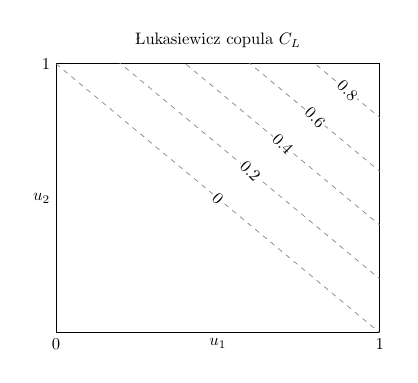
\begin{tikzpicture}[scale=0.6]
        \begin{axis}[
            xmin=0,xmax=1,
            ymin=0,ymax=1,
            xtick={0, 0.5, 1},
		    xticklabels={$0$, $u_1$, $1$},
		    ytick={0.5, 1},
		    yticklabels={$u_2$, $1$},
		    xtick style={draw=none},
		    ytick style={draw=none},
            title={\L ukasiewicz copula $C_L$},
            ]
            \addplot [domain=0:1,samples=40,style=dashed,color=gray]({x},{1-x});
            \addplot [domain=0:1,samples=40,style=dashed,color=gray]({x},{1.2-x}); 
            \addplot [domain=0:1,samples=40,style=dashed,color=gray]({x},{1.4-x}); 
            \addplot [domain=0:1,samples=40,style=dashed,color=gray]({x},{1.6-x}); 
            \addplot [domain=0:1,samples=40,style=dashed,color=gray]({x},{1.8-x});

            \node[rotate=-45, fill=white, rounded corners=2pt, inner sep=1pt] (x) at (0.5, 0.5) {0};
            \node[rotate=-45, fill=white, rounded corners=2pt, inner sep=1pt] (x) at (0.6, 0.6) {0.2};
            \node[rotate=-45, fill=white, rounded corners=2pt, inner sep=1pt] (x) at (0.7, 0.7) {0.4};
            \node[rotate=-45, fill=white, rounded corners=2pt, inner sep=1pt] (x) at (0.8, 0.8) {0.6};
            \node[rotate=-45, fill=white, rounded corners=2pt, inner sep=1pt] (x) at (0.9, 0.9) {0.8};
        \end{axis}
        \end{tikzpicture}\quad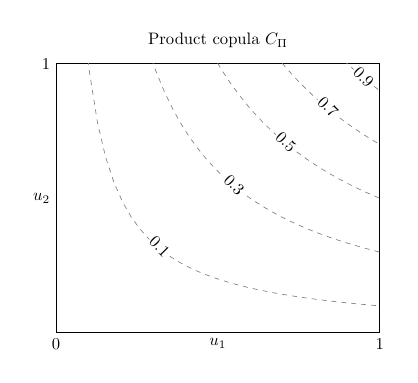
\begin{tikzpicture}[scale=0.6]
        \begin{axis}[
            xmin=0,xmax=1,
            ymin=0,ymax=1,
            xtick={0, 0.5, 1},
		    xticklabels={$0$, $u_1$, $1$},
		    ytick={0.5, 1},
		    yticklabels={$u_2$, $1$},
		    xtick style={draw=none},
		    ytick style={draw=none},
            title={Product copula $C_\Pi$},
            ]
            \addplot[domain=0:1,samples=40,style=dashed,color=gray]({x},{0.1/x});
            \addplot[domain=0:1,samples=40,style=dashed,color=gray]({x},{0.3/x}); 
            \addplot[domain=0:1,samples=40,style=dashed,color=gray]({x},{0.5/x}); 
            \addplot[domain=0:1,samples=40,style=dashed,color=gray]({x},{0.7/x}); 
            \addplot[domain=0:1,samples=40,style=dashed,color=gray]({x},{0.9/x});

            \node[rotate=-45, fill=white, rounded corners=2pt, inner sep=1pt] (x) at (0.32, 0.32) {0.1};
            \node[rotate=-45, fill=white, rounded corners=2pt, inner sep=1pt] (x) at (0.55, 0.55) {0.3};
            \node[rotate=-45, fill=white, rounded corners=2pt, inner sep=1pt] (x) at (0.71, 0.71) {0.5};
            \node[rotate=-45, fill=white, rounded corners=2pt, inner sep=1pt] (x) at (0.84, 0.84) {0.7};
            \node[rotate=-45, fill=white, rounded corners=2pt, inner sep=1pt] (x) at (0.95, 0.95) {0.9};
            
        \end{axis}
        \end{tikzpicture}\quad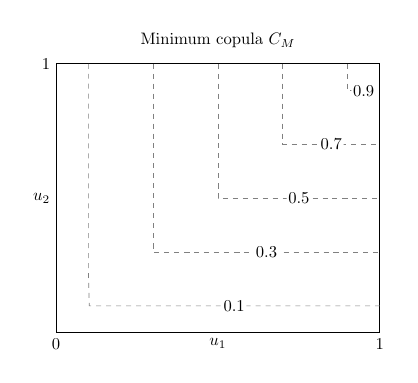
\begin{tikzpicture}[scale=0.6]
        \begin{axis}[
            xmin=0,xmax=1,
            ymin=0,ymax=1,
            xtick={0, 0.5, 1},
		    xticklabels={$0$, $u_1$, $1$},
		    ytick={0.5, 1},
		    yticklabels={$u_2$, $1$},
		    xtick style={draw=none},
		    ytick style={draw=none},
            title={Minimum copula $C_M$},
            ]
            \addplot [domain=0:1,samples=40,style=dashed,color=gray]({max(x, 0.1)},{max(1-x/0.1,0.1)});
            \addplot [domain=0:1,samples=40,style=dashed,color=gray]({max(x, 0.3)},{max(1-x/0.3,0.3)});
            \addplot [domain=0:1,samples=40,style=dashed,color=gray]({max(x, 0.5)},{max(1-x/0.5,0.5)});
            \addplot [domain=0:1,samples=40,style=dashed,color=gray]({max(x, 0.7)},{max(1-x/0.7,0.7)});
            \addplot [domain=0:1,samples=40,style=dashed,color=gray]({max(x, 0.9)},{max(1-x/0.9,0.9)});

            \node[fill=white, rounded corners=2pt, inner sep=1pt] (x) at (0.55, 0.1) {0.1};
            \node[fill=white, rounded corners=2pt, inner sep=1pt] (x) at (0.65, 0.3) {0.3};
            \node[fill=white, rounded corners=2pt, inner sep=1pt] (x) at (0.75, 0.5) {0.5};
            \node[fill=white, rounded corners=2pt, inner sep=1pt] (x) at (0.85, 0.7) {0.7};
            \node[fill=white, rounded corners=2pt, inner sep=1pt] (x) at (0.95, 0.9) {0.9};
        \end{axis}
        \end{tikzpicture}
    \caption{Bird view of the \L ukasiewicz, product and Min copulas for $n=2$. Dashed gray lines represent isolines of the copulas.}
    \label{fig:copulas}
\end{figure}


{\renewcommand{\arraystretch}{2}%
\begin{table}[!ht]
    \centering
    \begin{tabular}{|c|c|c|c|c|}
        \hline
        Family & $C(u_1,u_2)$ & $\theta \in $ & D-convex & D-concave \\
        \hline\hline
        Ali-Mikhail-Haq & $\frac{u_1u_2}{1-\theta(1-u_1)(1-u_2)}$ & $[-1,1)$ & $\theta\leqslant0$ & $0\leqslant\theta$ \\
        \hline
        Clayton & $\left[\max(u_1^{-\theta}+u_2^{-\theta}-1,0)\right]^{-1/\theta}$ & $[-1,\infty)\backslash\{0\}$ & $\theta<0$ & $0<\theta$ \\
        \hline
        Frank & $-\frac{1}{\theta}\ln(1+\frac{(e^{-\theta u_1}-1)(e^{-\theta u_2}-1)}{e^{-\theta}-1})$ & $\mathbb{R}\backslash \{0\}$ & $\theta<0$ & $0<\theta$ \\
        \hline
        Gumbel & $u_1u_2\exp(-\theta \ln{u_1}\ln{u_2})$ & $(0,1]$ & $\theta\in(0,1]$  & Never \\
        \hline
    \end{tabular}
    \caption{Examples of families of copulas in the case $n=2$ which can be generated using a parameter \( \theta \). D-convexity/concavity is detailed in \Cref{sec:dconvexity}}
    \label{tab:familiy_of_copula}
\end{table}}\commanue{alors la notation $0\leqslant\theta$ c'est pas la plus lisible disons qu'on a plutôt tendance à mettre $\theta\geqslant 0$ }

\begin{remark}
	As a copula is also a multivariate CDF, one can imagine an ``imprecise'' copula similarly to what can be done with univariate probability distribution (see \Cref{sec:imprecise_probabilities}). Imprecise copula allow to model partially known dependencies, but can be hard to manipulate at times, as for instance the lower and upper bounds of an imprecise copula are not necessarily copulas themselves. In this thesis, we will not consider imprecise copulas.
\end{remark}

\subsection{Directional convexity/concavity for copulas}\label{sec:dconvexity}
This section will investigate a property shared by some copulas called directional convexity/concavity. This is more of a theoretical contribution\commanu{this is a theoritical, pas besoin du more of. peut etre dire clairement que tu l'as faite? et que cela t'a servi à mieux appréhender ce champ math de l'incertitude?}, as we do not exploit them in the applications to stereophotogrammetry in chapters \ref{chap:propagating} and \ref{chap:epistemic_uncertainty}. However, we will see that those properties are shared by many common families of copulas. We also use them to prove a specific relationship between multivariate uncertainty models in sections \ref{subsec:pboxes} and \ref{subsec:multiple_models}. For readers that do not want to dive into details regarding directional convexity/concavity, we advise to consider only definition \ref{def:convex} and the main result of this section which is presented in \cref{eq:convex_diff_hvol}.

\begin{definition}[D-convexity, D-concavity]\label{def:convex}
    A copula $C$ is called directionally convex (D-convex) \cite{alvoni_dierent_2007} if for every $(u_1 \enum u_n)\in[0,1]^n$, $(v_1\enum v_n)\in[0,1]^n$, $i\in\opi1,n\cli$ and $t\in[0,1]$ it verifies:
    \begin{align}
        C(u_1\enum tu_i+(1-t)v_i\enum u_n) ~\leqslant~&t\cdot C(u_1\enum u_i\enum u_n)\nonumber\\
        &+ (1-t)\cdot C(u_1\enum v_i\enum u_n)\label{eq:convex_copula}
    \end{align}
    In other words, the copula is convex when fixing all but one of its variables. A copula is called directionally concave (D-concave) if the inequality is reversed.
\end{definition}

\begin{remark}
    D-convexity/D-concavity is quite common in known families of copulas. The following paragraphs details this property for copulas presented in \Cref{tab:familiy_of_copula}, in the case $n=2$.
    As the copulas presented are symmetric regarding their variables, D-convexity/D-concavity is only detailed for $u_1$. We assume that \( \theta \) always belong to the domain of definition detailed in \Cref{tab:familiy_of_copula}, and that \(u_1, u_2\) are in \([0, 1]\). Finally, for the Clayton and Gumbel family, the copula is defined by continuous extension in cases $u_1=0$ and $u_2=0$. 
    \begin{description}
        \item[Ali-Mikhail-Haq copula] This copula is two times differentiable, and its second order partial derivative is
        $$\frac{\partial^2 C}{\partial {u_1}^2}=u_2(1-\theta(1-u_2))\frac{-2\theta(1-u_2)}{(1-\theta(1-u_1)(1-u_2))^3}$$
        Thus the Ali-Mikhail-Haq copula is D-convex for $\theta\in[-1,0]$ and D-concave for $\theta\in[0,1)$.\commanue{Peut-être ajouter quelque part, la copule est convexe si et seulement si sa dérivée seconde est à valeurs positives ou nulles. }\comloic{ouais parce que j'avoue que j'ai du faire un passage par wikipedia :s}
        \item[Clayton copula] This copula is not always differentiable on all of its domain, depending on the value retained in the maximum function. It is however continuous as it is the maximum of two continuous function. For convenience, we work with $(u_1, u_2)$ in $\mathbb{I}^2$, where $\mathbb{I}$ is the open unit interval (the closed unit interval is then covered by continuity). Let $u_2\in\mathbb{I}$. We split the possible range $\mathbb{I}$ of $u_1$ in two:
    \begin{itemize}
        \item the first domain $\mathcal{D}_1^{\theta,u_2}$ is where $u_1^{-\theta}+u_2^{-\theta}-1\leqslant0$, and thus $C(u_1, u_2)=0$. Here, $\frac{\partial^2 C}{\partial {u_1}^2}=0$ and the copula is both D-convex and D-concave.
        \item the second domain $\mathcal{D}_2^{\theta,u_2}$ is where $u_1^{-\theta}+u_2^{-\theta}-1>0$ and thus $C(u_1, u_2)\geqslant0$. Here it holds that
        $$\frac{\partial^2 C}{\partial {u_1}^2}=(1+\theta)(1-u_2^{-\theta})u_1^{-2-\theta}(u_1^{-\theta}+u_2^{-\theta}-1)^{-2-\frac{1}{\theta}}$$
        Because of the definition of $\mathcal{D}_2^{\theta,u_2}$, the sign of $\frac{\partial^2 C}{\partial {u_1}^2}$ on $\mathcal{D}_2^{\theta,u_2}$ is that of $1-u_2^{-\theta}$.
    \end{itemize}
    
    If $\theta>0$, then $D^\theta_2=\mathbb{I}$ and $\frac{\partial^2 C}{\partial {u_1}^2}\leqslant0$ which means that the copula is D-concave on all of its domain.
    
    The case where $\theta<0$ is less straightforward. In that case, $\frac{\partial^2 C}{\partial {u_1}^2}\geqslant0$ on $\mathcal{D}_2^{\theta,u_2}$. The restrictions of the copula to $\mathcal{D}_1^{\theta,u_2}$ and $\mathcal{D}_2^{\theta,u_2}$ are both D-convex, but we need to prove that it is still true on their union. Let $u_1\in\mathcal{D}_1^{\theta,u_2}$, $v_1\in\mathcal{D}_2^{\theta,u_2}$ and $t\in[0,1]$. We note $w_1=(1-u_2^{-\theta})^{-\frac{1}{\theta}}$, such that $\mathcal{D}_1^{\theta,u_2}=]0,w_1]$ and $\mathcal{D}_2^{\theta,u_2}=]w_1, 1[$. By continuity, $C$ is D-convex on $\mathcal{D}_2^{\theta,u_2}\bigcup\{w_1\}$. Because $u_1,w_1\in \mathcal{D}_1^{\theta,u_2}$, it holds that:
        \begin{eqnarray*}
            tC(u_1,~u_2)+(1-t)C(v_1,~u_2) &=& tC(w_1,~u_2)+(1-t)C(v_1,~u_2)\\
            &\geqslant& C(tw_1+(1-t)v_1,~u_2)\\
            &&\text{by convexity of $C$ on $\mathcal{D}_2^{\theta,u_2}\bigcup\{w_1\}$}\\
            &\geqslant& C(tu_1+(1-t)v_1,~u_2)\\
            && \text{because $C$ is component-wise increasing}
        \end{eqnarray*}
    which, by definition \ref{def:convex}, proves that $C$ is D-convex on $\mathcal{D}_1^{\theta,u_2}\bigcup \mathcal{D}_2^{\theta,u_2}$. By continuity, $C$ is D-convex on all of its domain.
    \item[Frank copula] This copula is two times differentiable, and its second order partial derivative is
    $$\frac{\partial^2 C}{\partial {u_1}^2}=\frac{(e^{-\theta u_2}-1)e^{-\theta u_1}\theta(e^{-\theta u_2}-e^{-\theta} )}{(e^{-\theta}-1+(e^{-\theta u_1}-1)(e^{-\theta u_2}-1))^2}$$
    If $\theta\geqslant0$ then $\frac{\partial^2 C}{\partial {u_1}^2}\leqslant 0$ and $C$ is D-concave. If $\theta\leqslant0$ then $\frac{\partial^2 C}{\partial {u_1}^2}\geqslant 0$ and $C$ is D-convex.
    \item[Gumbel copula] This copula is two times differentiable on $]0,1]^2$, and its second order partial derivative is
    $$\frac{\partial^2 C}{\partial {u_1}^2}=-\theta\frac{u_2}{u_1}\ln(u_2)(1-\theta\ln(u_2))e^{-\theta\ln(u_1)\ln(u_2)}$$
    It holds that for all $\theta\in(0,1]$, $\frac{\partial^2 C}{\partial {u_1}^2}\geqslant0$. By continuity, $C$ is always D-convex.
    \end{description}
    
    As there is no explicit formula for the family of multivariate Gaussian copulas, it is difficult to prove its D-concavity or D-convexity. However, numerical approximations in the case $n=2$ seem to indicate that a Gaussian copula would be D-convex if its marginals are positively correlated, and D-concave if they are negatively correlated. \Cref{fig:gaussian_copula_simu} present those observations, with solid lines representing positive correlation, and dashed lines representing negative correlations. In the case $n>2$, the copula can be neither D-convex nor D-concave depending on the value of the correlation matrix. An example of this statement is provided in \Cref{fig:gaussian_copula_simu_n3}.
\end{remark}

\begin{figure}
    \centering
    \begin{subfigure}{0.4\linewidth}
        \centering
        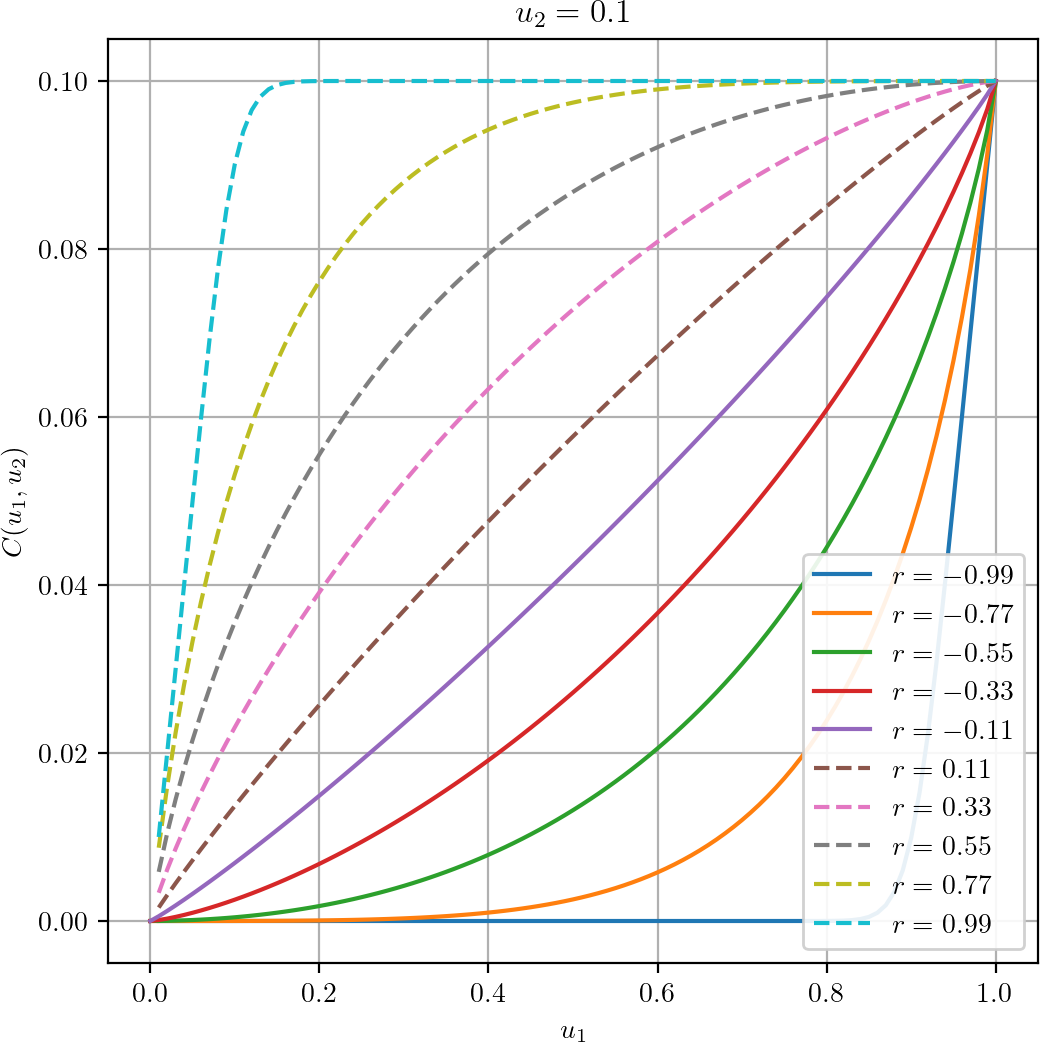
\includegraphics[width=\linewidth]{Images/Chap_2/Gaussian_copula/gaussian_copula_0.png}
    \end{subfigure}\hfill
    \begin{subfigure}{0.4\linewidth}
        \centering
        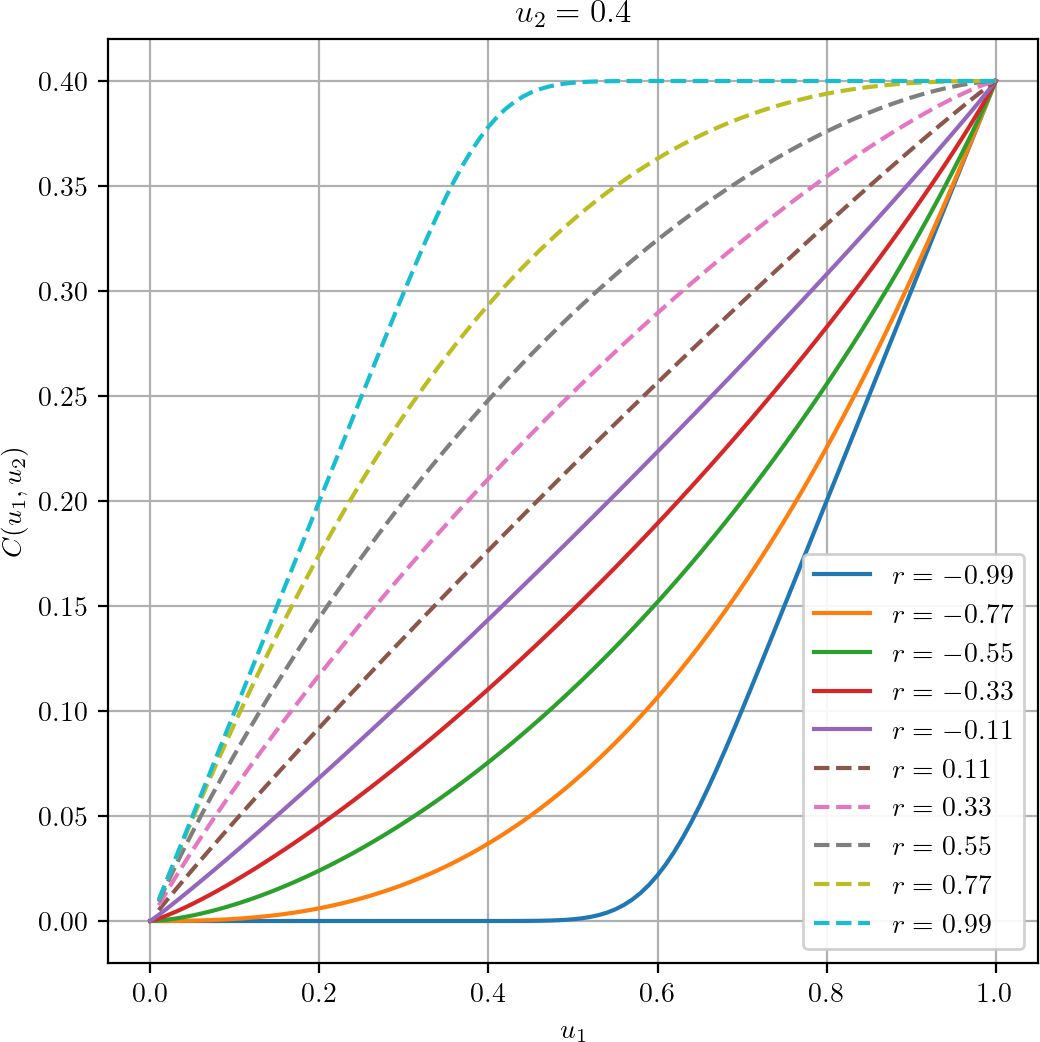
\includegraphics[width=\linewidth]{Images/Chap_2/Gaussian_copula/gaussian_copula_1.png}
    \end{subfigure}\hfill
    \begin{subfigure}{0.4\linewidth}
        \centering
        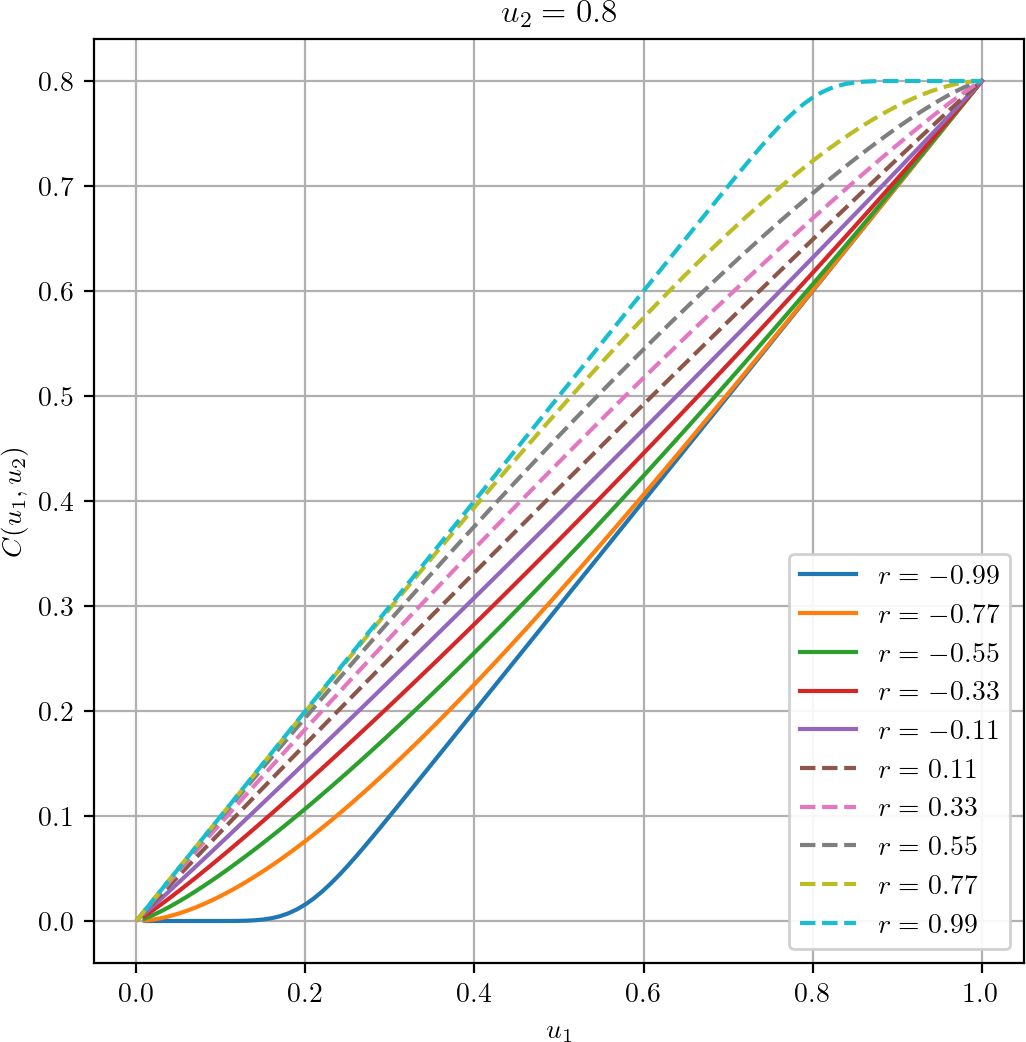
\includegraphics[width=\linewidth]{Images/Chap_2/Gaussian_copula/gaussian_copula_2.png}
    \end{subfigure}
    \caption{Gaussian 2-copulas in the direction $u_1$ for different $u_2$. Each figure present different plots for correlations $r$ between $u_1$ and $u_2$ ranging in $[-1,1]$. Solid lines represent negative correlation, while dashed lines represent positive correlations.}
    \label{fig:gaussian_copula_simu}
\end{figure}

The rest of this section will present different results regarding D-convex and D-concave copulas, leading to the main result of this section presented in proposition \ref{prop:convex_diff_hvol}.

\begin{figure}
    \centering
    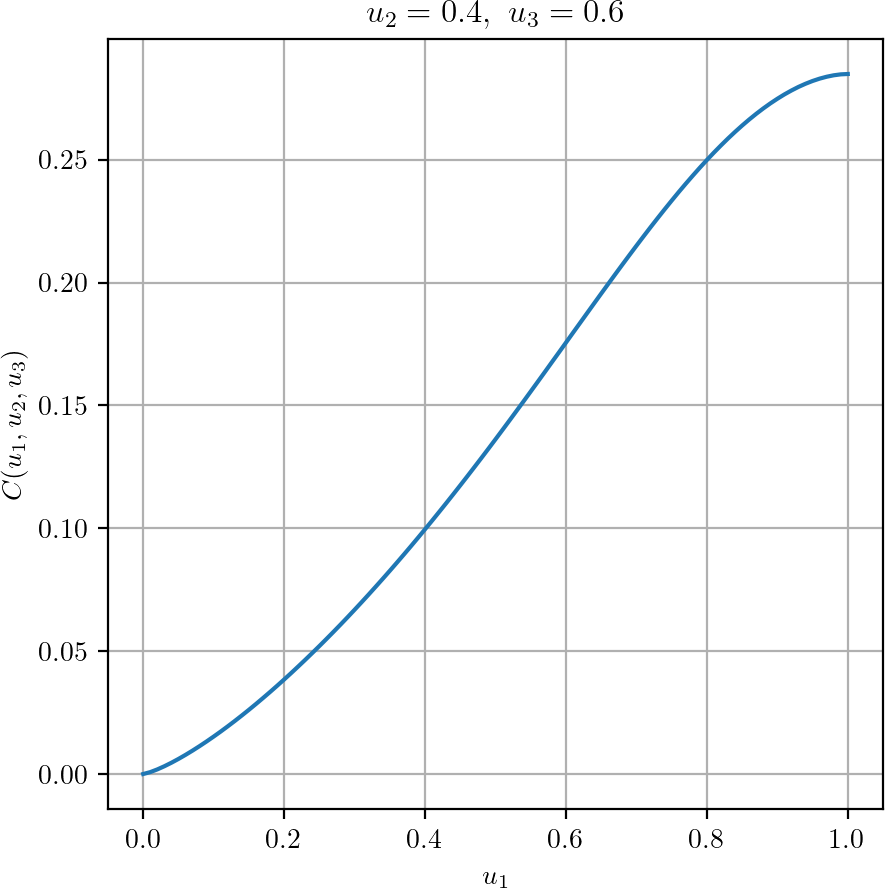
\includegraphics[width=0.5\linewidth]{Images/Chap_2/Gaussian_copula/gaussian_copula_n3.png}
    \caption{Directional cut of a Gaussian 3-copula with in the direction $u_1$, with $R=\begin{bmatrix} 1 & -0.4 & 0.7\\ -0.4 & 1 & 0.3\\ 0.7 & 0.3 & 1 \end{bmatrix}$, $u_2=0.4$ and $u_3=0.6$. The copula is neither D-convex nor D-concave}
    \label{fig:gaussian_copula_simu_n3}
\end{figure}

\begin{remark}
    All D-convex copulas $C$ are dominated by the product copula. Similarly, all D-concave copulas dominate the product copula.

    Consider a D-convex copula $C$, and let $(u_1\enum u_n)\in[0,1]^n$.
    \begin{eqnarray*}
        C(u_1\enum u_n) &=& C((1-u_1)\cdot0+u_1\cdot 1, u_2\enum u_n)\\
        &\leqslant& (1-u_1)C(0, u_2\enum u_n)+u_1C(1, u_2\enum u_n)\\
        &=& u_1C(1, u_2\enum u_n)\commanue{alors moi je laisserais le symbole $\leqslant$ et pas $=$}
    \end{eqnarray*}
    Doing the same for $u_2\enum u_n$ yields:
    \begin{eqnarray*}
        C(u_1\enum u_n) &\leqslant& u_1\dots u_nC(1\enum1) = u_1\dots u_n = C_\Pi(u_1\enum u_n)
    \end{eqnarray*}
    The proof for D-convexity is similar.
\end{remark}

\begin{proposition}\label{prop:sup_additivity}
    If $C$ is a D-convex copula, then it verifies for all $(u_1\enum u_n)\in[0,1]^n$, $(v_1\enum v_n)\in[0,1]^n$ \st $\forall i\in\opi1,n\cli$, $u_i+v_i\leqslant 1$:
    \begin{eqnarray}
        C(u_1\enum u_i+v_i\enum u_n)\geqslant& &C(u_1\enum u_i\enum u_n)\nonumber\\
        &+ &C(u_1\enum v_i\enum u_n)\label{eq:convex_sum}
    \end{eqnarray}
    Similarly, if $\forall i\in\opi1,n\cli$, $u_i-v_i\geqslant 0$, it verifies:
    \begin{eqnarray}
        C(u_1\enum u_i-v_i\enum u_n)\leqslant& &C(u_1\enum u_i\enum u_n)\nonumber\\
        &- &C(u_1\enum v_i\enum u_n)\label{eq:convex_diff}
    \end{eqnarray}
    The inequalities are reversed for D-concave copulas.
\end{proposition}

\begin{proof}
    Let $(u_1\enum u_n)\in[0,1]^n$, $(v_1\enum v_n)\in[0,1]^n$ \st $\forall i\in\opi1,n\cli$, $u_i+v_i\leqslant 1$. Let $i\in\opi1,n\cli$. Applying the definition of convexity \eqref{eq:convex_copula} with $v_i=0$ yields:
    \begin{eqnarray*}
        \forall t\in[0,1],~C(u_1\enum tu_i\enum u_n) \leqslant tC(u_1\enum u_n)
    \end{eqnarray*}
    
    Let $w_i=u_i+v_i\in ]0,1]$ (the case where $u_i=0$ or $v_i=0$ is trivial). It is possible to write $u_i=tw_i$ and $v_i=(1-t)w_i$, with $t=\frac{u_i}{w_i}\in[0,1]$. Then it holds that:
    \begin{eqnarray*}
            C(u_1\enum u_i\enum u_n) =& C(u_1\enum tw_i\enum u_n) &\leqslant tC(u_1\enum w_i\enum u_n)\\
            C(u_1\enum v_i\enum u_n) =& C(u_1\enum (1-t)w_i\enum u_n) &\leqslant (1-t)C(u_1\enum w_i\enum u_n)
    \end{eqnarray*}
    Summing the above equations yields:
    \begin{eqnarray*}
        C(u_1\enum u_i\enum u_n) + C(u_1\enum v_i\enum u_n) &\leqslant& C(u_1\enum w_i\enum u_n)\\
        &\leqslant& C(u_1\enum u_i+v_i\enum u_n)
    \end{eqnarray*}
    which proves \cref{eq:convex_sum}.

    Let $w_i=u_i-v_i\in [0,1]$, clearly $w_i+v_i\leqslant1$. Using \cref{eq:convex_sum}, it holds that:
    \begin{align*}
        &C(u_1\enum w_i\enum u_n) + C(u_1\enum v_i\enum u_n) &\leqslant~&C(u_1\enum w_i+v_i\enum u_n)\\
        \Leftrightarrow~ &C(u_1\enum w_i\enum u_n) &\leqslant~&C(u_1\enum w_i+v_i\enum u_n)\\
        &&&-C(u_1\enum v_i\enum u_n)\\
        \Leftrightarrow~ &C(u_1\enum u_i-v_i\enum u_n) &\leqslant~&C(u_1\enum u_i\enum u_n)\\
        &&&-C(u_1\enum v_i\enum u_n)
    \end{align*}
    which proves \cref{eq:convex_diff}.
\end{proof} 

\begin{proposition}\label{prop:convex_diff_hvol}
    If $C$ is a D-convex copula, then it verifies for all $(u_1\enum u_n)\in[0,1]^n$, $(v_1\enum v_n)\in[0,1]^n$ \st $\forall i\in\opi1,n\cli$, $u_i-v_i\geqslant 0$:
    \begin{eqnarray}
        C(u_1-v_1\enum u_i-v_i\enum u_n-v_n)\leqslant& &H^{u_1\enum u_i\enum u_n}_{v_1\enum v_i\enum v_n}\label{eq:convex_diff_hvol}
    \end{eqnarray}
    where $H$ is the H-volume of $C$. The inequality is reversed for D-concave copulas.
\end{proposition}

\begin{proof}
    The result is straightforward by induction using \cref{eq:convex_diff}.
\end{proof}

\subsection{Sampling from a Copula}\label{sec:sampling_copula}
As a copula represent the CDF of a multivariate random variable, it is possible to sample from it. This section details a method for sampling from copulas in general, and a special method for sampling from Gaussian copulas. \commanu{question béotien: est ce que ca te sert après ou idem c'est pour la théorie. Tu l'as fait de mettre une phrase de contexte par rapport à ta thèse, peut etre bien ici aussi pour "sampling from copula"} For simplicity, let us first present a method for sampling in the case $n=2$. Given a copula $C$, and two CDF $F_X$ and $F_Y$, a method to generate a pair of observations $(x, y)$ from a joint CDF $C(F_X, F_Y)$ is the following:

\begin{itemize}
    \item Sample two independent samples $u_1, u_2$ from a uniform distribution on [0,1]
    \item Set $v=\partial C^{-1}(u_2)$ where $\partial C^{-1}$ is the quasi-inverse of the partial derivative of $C$ regarding its first variable (which exists almost everywhere and is invertible).
    \item We now have a sample $(u_1, v)$ from a multivariate random. Its marginals follow a uniform distribution on $[0,1]$, and its associated copula is $C$.
    \item The desired pair is $(x_1,x_2) = (F^{-1}_X(u_1), F^{-1}_Y(v))$, with $F_X^{-1}$, $F_Y^{-1}$ being the quasi-inverses of the marginals CDFs.
\end{itemize}

We do not present the $n$-dimensional general case here as it is a bit more complex, but it can be found in \cite{cherubini_copula_2004}. However, drawing samples from a Gaussian $n$-copula with a correlation matrix $R$ are simpler to obtain:
\begin{itemize}
    \item Compute the Cholesky decomposition $A$ of the correlation matrix $R$
    \item Draw $n$ independent random samples $u=(u_1\enum u_n)'$ from $\mathcal{N}(0,1)$, where $\mathcal{N}$ is the normal distribution.
    \item Set $v=Au$
    \item Set $w_k=\Phi(v_k)$ where $\Phi$ is the univariate normal cumulative distribution function
    \item The desired draw is $(x_1\enum x_n)=(F^{-1}_1(w_1)\enum F^{-1}_n(w_n))$ with $F_i^{-1}$, being the quasi-inverse of the $i$-th marginal CDF.
\end{itemize}
\commanue{Alors il manque une conclusion un truc, là ça termine un peu de manière abrupte, transition donc ;)}\comloic{+1 ne serait ce qu'un badge ou un remerciement pour avoir atteint la fin du chapitre ;-) (avec un encouragement avant le prochain)... là je me sens devant le chapitre 3 un peu comme devant le panneau 10km du sommet à la moitié du tourmalet quand tu sais que la haut c'est encore bien raide. J'hésite entre poser le pied à terre, enfiler des tongues et lire le chapitre 4 tranquilou sur une place de café au risque de me tromper de direction en repartant et plus jamais trouver le courage de faire le 3, ou bien continuer avec acharnement sur le 3 juste par fierté en faire une histoire entre les copules et moi. Le truc c'est que s'il y a pas un monument une boutade ou quoi à la fin du chapitre 3 ça va pas être super gratifiant ^^'}


\pagebreak
\blankpage

\chapter{Propagating the Uncertainty of Stereo Images}\label{chap:propagating}
This chapter details the work conducted on the propagation of uncertainty from images into the cost curves of dense matching problems. We consider a simple model of uncertainty on the input images, a dependency model between the uncertain intensities of the images, and estimate the resulting uncertainty on the output cost curves. This chapter takes up work and data already published \cite{malinowski_copulas_2022, malinowski_uncertainty_2023, malinowski_robust_2024}.

\section{Sources of Uncertainty in Stereo Matching}\label{sec:sources_of_uncertainty}
\todoroman{Points à aborder: Atmospheric correction, vibration, resolution of a pixel, discretization.
CO3D mission will not have the epipolar line correction problem that is encountered with pleiades images.
Epipolar line rectification for Pléiades is a problem that is not dealt here.}

To maintain simplicity in this section, we will not consider panchromatic images, such as Pléiades products, encoding the reflectance values as positive integer, usually contained in $[0, 5000]$. Instead, we consider grayscale images that have intensity levels quantified within the range $[0, 255]$, which will represent our measurable space $\X$. We hypothesize that a pixel's intensity value can deviate by no more than $1$ level from its observed value, with the observed value being the most likely. This hypothesis arises from the noise of the sensor capturing the image, from pre-processing steps (see section \ref{sec:classical_stero_pipeline}) or from the quantification of observed radiometric values into integers. We assume this simple hypothesis to keep our explanation straightforward. Consequently, we model the uncertainty of each pixel $p\in I_L,I_R$ intensity with a possibility distribution $\pi$, centered around the observed intensity $i_p\in[0,255]$:
\begin{equation}
    \pi(i_p)=1,\quad \pi(i_p\pm1)=\alpha\,,
\end{equation}\label{eq:pixel_possibility}
with $\alpha \in [0,1]$. The $\pm$ indicates that both positive and negative values are considered. In our simulation, $\alpha = 0.3$ for pixels in the left image and $\alpha = 0.4$ for pixels in the right image. We use different values of $\alpha$ for the left and right images because the uncertainty model may vary between images due to differences in exposure, noise levels, or camera calibration. This model effectively states that we accept any probability distribution supported within $[i_p - 1, i_p + 1]$ where the probability measure $P$ satisfies $\{P(A) \leq \sup_{i \in A} \pi(i)\}$ as an acceptable model for our uncertainty. The mass distribution function $m_p$ associated to this credal set possesses two focal sets $a^p$:
\begin{eqnarray}
    &m_p(a^p_1=\opi i_p, i_p\cli)=1-\alpha\,\nonumber\\
    &m_p(a^p_2=\opi i_p-1, i_p + 1\cli)=\alpha\,\label{eq:pixel_mass}
\end{eqnarray}
with $\opi\cdot, \cdot\cli$ referring to integer intervals. In particular, $\opi i_p, i_p\cli$ correspond to the singleton $\{i_p\}$.

It is important to note that in this disparity estimation problem, we only account for the uncertainty in our input image intensities, without considering the uncertainty in our cost function's ability to correctly identify the true disparity as its minimum. In other words, we do not account for the uncertainty arising from the difference between ``two patches are very similar'' and ``the pixels at the center of the patches are homologous''. To better illustrate this, imagine a scenario where two pixels should be matched, but the surrounding patches are dissimilar. In this case, the cost function between those two patches would be high, potentially leading to the selection of a different patch with a lower cost function as the estimated disparity. The correct disparity would not be the minimum of the cost curve. This problem tends to appear more often when considering large windows, as the cost function can `average' the similarity of all its pixels, regardless of the similarity of the central ones. 

We consider the Sum of Absolute Differences (SAD) as our cost function, defined as follows. Given patches $W_L\subset I_L$ and $W_R\subset I_R$ of the same shape with $n$ pixels (usually squares):
\begin{align}
    \mathrm{SAD}(W_L, W_R) = \sum_{(p_i, q_i)\in (W_L, W_R)}|I_L(p_i) - I_R(q_i)|\label{eq:SAD}
\end{align}
where $p_i$ and $q_i$ are pixels at the same position $i$ in their patch. For convenience purposes, we will refer to the Absolute Difference as AD. This cost function is not ideal compared to more complex state-of-the-art cost function (\cite{zbontar_stereo_2016}, \cite{laga_survey_2022}), but it is preferred here to focus on simplicity and to ease didactic explanations regarding uncertainty propagation. An illustration of the SAD cost function can be found in Figure \ref{fig:SAD}. Furthermore, we will not consider in this chapter the use of Semi Global Matching (or similar regularization methods), as it necessitates many operations due to its recursive formulation and thus greatly increases complexity for the uncertainty propagation. We diverge from state-of-the-art methods to keep explanations as simple as possible, however the modeling of uncertainty for more advanced cost functions and SGM methods will be considered in chapter \ref{chap:epistemic_uncertainty}.

An ideal cost function would generate a cost curve with a unique minimum corresponding to the correct disparity. In practice, such a function is hard to determine. There is no guarantee that the minimum is unique, nor that it corresponds to the correct disparity. 

\begin{figure}
    \centering
    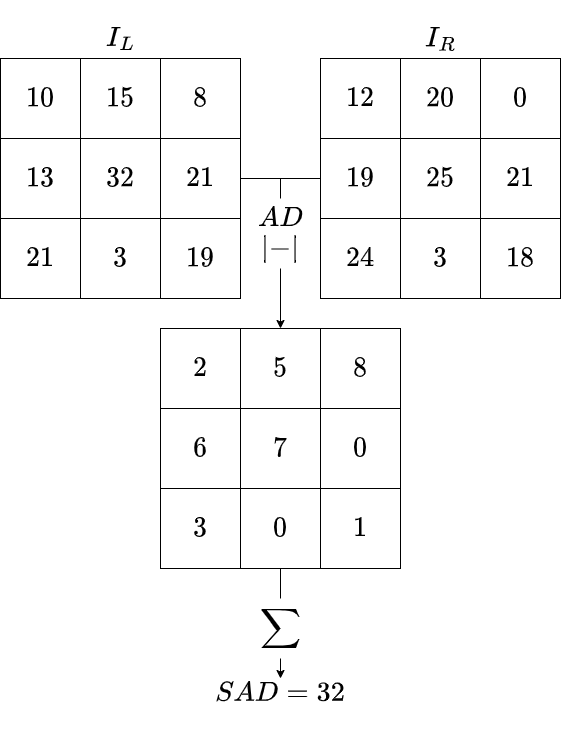
\includegraphics[width=0.5\linewidth]{Images/SAD.png}
    \caption{Diagram representing the $SAD$ cost function between two $3\times3$ patches.}
    \label{fig:SAD}
\end{figure}

We presented the uncertainty models for pixels in both images, but we also need to define the dependency model between every pixels of both images. In our case, we propose to model their dependency with the product copula if the pixels are not from the same physical object (meaning that the value of their intensities are independent), and by a Gaussian copula with a covariance matrix parameterized by a correlation matrix $R$. The correlation between the uncertain pixel intensities is based on a segmentation $S:(I_L\cup I_R)\rightarrow[\![0,K]\!]$, $K\in\mathbb{N}$, of the images, performed on the ground truth disparity of each pixel. Given two pixels $(p, q)\in(I_L\cup I_R)^2$, their covariance is determined by:
\begin{equation}
    \mathrm{cov}(p, q) =
    \begin{cases}
        1 &\text{ if }p=q\,,\\
        \rho_k, &\text{ if } p\ne q\text{ and }S(p)=S(q)\,, \\
        0, & \text{otherwise}\,.
    \end{cases}\label{eq:correlation}
\end{equation}
During the simulations, the segmentation contains $K=8$ different clusters, and for every $k$ in $[\![0,K]\!]$, $\rho_k$ is assigned an arbitrary value between $0.9$ and $1$.

We can thus build a correlation matrix $R$ for all pixels of $(I_L\cup I_R)$, and sample a perturbation on all of the pixels using a Gaussian copula with this correlation matrix. The Gaussian $18-$copula used to model the dependency between marginal masses in the uncertainty propagation step (using equation \eqref{eq:joint_mass}) is also constructed using Equation \eqref{eq:correlation}. 

\section{Propagation of the Uncertainty with Belief Functions}
This section will present how we can compute a Belief function on the matching cost curve values from the original beliefs as well as a copula representing the dependency between variables. We first detail how it can be done in the precise case, as the imprecise setting is similar. We use the case of the SAD cost function to illustrate the process.

First, let us present the propagation of uncertainty in the precise bivariate case. Let $f:\X_1\times\X_2\rightarrow\mathcal{Z}$ be a mapping and we define the random variables $Z$ as $Z=f(X,Y)$. 
When considering precise probabilities, the mass distribution $p_Z$ on atoms of $Z$ is:
\begin{align}
    \forall z\in\mathcal{Z}, p_Z(z)=\sum_{\substack{x_1,x_2\\z=f(x_1,x_2)}}p(x_1,x_2).
\end{align}

Determining every $(x,y)$, whose image by $f$ equals $z$, is not always trivial. This becomes even more complex when we are considering copulas with $n>2$ variables. Note that the joint probability $p(x_1,x_2)$ is computed using a H-volume, which is the sum of $2^n$ terms, also increasing exponentially with the dimension. In the continuous case, the H-volume is replaced with the density $h$ of the joint CDF. The density of $Z$ is thus:
\begin{align}
    p_Z(z) = \int_{\X_1}\int_{\X_2}h(x_1,x_2)\mathds{1}(f(x_1,x_2)=z)dx_1dx_2,
\end{align}
Here, $\mathds{1}$ refers to the characteristic function.

Similarly, belief functions can be propagated by replacing the mass on atoms with the mass associated to the joint belief function. Given the joint mass distribution function $m_\times$ constructed with a copula as in equation \eqref{eq:joint_mass}, it is possible to compute the mass distribution function $m_Z$ of a random set $Z$ from $n$ marginal random sets:
\begin{align}
    \forall a^Z\subseteq\mathcal{Z}, m_Z(a^Z) = \sum_{\substack{a^1_i, \dots, a^n_j\\a^Z=f(a^n_1,\dots, a^n_j)}}m_\times(a^1_i, \dots, a^n_j)\label{eq:mass_propagated}
\end{align}
Computing the image of $f$ for every pair of focal sets $(a^1_i, \dots, a^n_j)$ is even more difficult than in the precise case, as we are computing reverse images of sets instead of real numbers. Propagation of uncertainty with a copula has also been investigated in the case of necessity functions in \cite{gray_dependent_2021}. To illustrate how to propagate the uncertainty using belief functions and a copula, we will use the SAD cost function as an example.

The SAD is used to compute the similarity between $3\times3$ windows $W_L, W_R$. We use the mass distribution $m_p$ of Equation \eqref{eq:pixel_mass} to represent the uncertainty of each pixel $p$. For every pair of pixels $p\in I_L, q\in I_R$, we note $\mathrm{AD}_{pq}=|i_p - i_q|$. There exists $3$ focal sets related to the absolute difference:
\begin{itemize}
    \item $a^{\mathrm{AD}}_1$ is the image of the AD of $a^p_1$ and $a^q_1$
    \item $a^{\mathrm{AD}}_2$ is the image of the AD of $a^p_2$ and $a^q_1$ or $a^p_1$ and $a^q_2$
    \item  $a^{\mathrm{AD}}_3$ is the image of the AD of $a^p_2$ and $a^q_2$
\end{itemize}
The non-monotonicity of the absolute value around $0$ needs to be taken into account to compute their exact image through the AD:
\begin{align*}
    a^{\mathrm{AD}}_1&=\opi\mathrm{AD}_{pq},~\mathrm{AD}_{pq}\cli\,,\\
    a^{\mathrm{AD}}_2&=\opi\mathrm{AD}_{pq} - 1,~\mathrm{AD}_{pq} + 1\cli\text{ if }\mathrm{AD}_{pq}>0\,,\\
            &=\opi\mathrm{AD}_{pq},~\mathrm{AD}_{pq} + 1\cli\text{ otherwise }\,,\\
    a^{\mathrm{AD}}_3&=\opi\mathrm{AD}_{pq} - 2,~\mathrm{AD}_{pq} + 2\cli\text{ if }\mathrm{AD}_{pq}>1\,,\\
            &=\opi\mathrm{AD}_{pq} - 1,~\mathrm{AD}_{pq} + 2\cli\text{ if }\mathrm{AD}_{pq}=1\,,\\
            &=\opi\mathrm{AD}_{pq},~\mathrm{AD}_{pq} + 2\cli\text{ otherwise}\,.
\end{align*}

Bounds of the AD are then summed to obtain the final values of the SAD focal sets. The mass $m_{\mathrm{SAD}}$ of those focal sets are computed using equations \eqref{eq:joint_mass} and \eqref{eq:mass_propagated}. To represent the dependency between pixels of both windows, a Gaussian $18$-copula is used. Splitting the problem using lower dimension copulas is tempting, similarly to what can be done with vine copulas (\cite{czado_vine_2022}). However this is a complex problem that will not be explored in this thesis. We will instead work with Gaussian copulas, introducing a simple method for creating a correlation matrix. This will also allow us to present simple optimisation to reduce computation complexity and splitting the copulas into mutually independent groups of variables. 

\section{Leveraging Specificities to Accelerate Computations}
\todoroman{H Volume etc for SAD example, see IJAR.}

Determining the bounds of the SAD focal sets is mostly straightforward. However, computing the joint mass over two $3 \times 3$ windows is significantly more complex. For each combination of marginal focal sets, the mass $m_{\mathrm{SAD}}$ is computed using the $H$-volume of an $18$-copula, involving a sum of $2^{18}$ terms. Given that the uncertainty for each pixel is represented by $2$ focal sets, we need to evaluate $2^{18}$ combinations of these focal sets in total. This computation can thus become quite costly in memory and computation time, especially when computing it over a whole image. A strategy to reduce computation time is to leverage the fact that the focal sets derived from a possibility distribution (or equivalently from its necessity measure) form a nested family of sets. For simplicity, the following observations will be detailed in the case where there are $n=2$ sources of uncertainty to join, but they hold for every $n\geqslant2$. Propagating two necessity measures $\mathrm{Nec}_1:2^{\X_1} \rightarrow [0,1]$ and $\mathrm{Nec}_2: 2^{\X_2} \rightarrow [0,1]$ through a mapping $f: \X_1 \times \X_2 \rightarrow \mathcal{Z}$ using a copula $C$ does not generally result in a necessity measure, but rather a belief function.

For the special case where:
\begin{itemize}
    \item $\mathrm{Nec}_1$ and $\mathrm{Nec}_2$ are defined by symmetric uni-modal possibility distributions (typically triangular possibilities)
    \item $f$ is a monotone function applied to a linear combination $\alpha X_1 + \beta X_2 + \gamma$, with $(\alpha, \beta, \gamma) \in \mathbb{R}^3$
\end{itemize}
then the focal sets of $\mathrm{Nec}_{X_1}$ and $\mathrm{Nec}_{X_2}$ are families of nested sets that can be represented as:
\begin{align*}
    [\overline{X}_1-\delta x^1_i, \overline{X}_1+\delta x^1_i]\quad[\overline{X}_2-\delta x^2_j, \overline{X}_2+\delta x^2_j]
\end{align*}
with $\overline{X}_1\in\X_1,~\overline{X}_2\in\X_2$ and $\delta x^1_i,~\delta x^2_j$ positive scalars. This results in the focal sets $a_{ij}$ of $Z = f(X_1, X_2)$ having the following expression:
\begin{align*}
    a_{ij} = \left[ \alpha \overline{X_1} + \beta \overline{X_2} + \gamma - (|\alpha| \Delta x^1_i + |\beta| \Delta x^2_j), \right. \\
                 \left. \alpha \overline{X_1} + \beta \overline{X_2} + \gamma + (|\alpha| \Delta x^1_i + |\beta| \Delta x^2_j) \right],
\end{align*}
Those focal sets form a nested family of sets, which is a characteristic of necessity measures \cite{shafer_mathematical_1976}. When a monotone function is applied to these focal sets, the nesting property is maintained, although the symmetry of the sets might be lost. This implies that $\mathrm{Bel}_Z$ (the belief function derived from $Z$) behaves as a necessity measure under these conditions.

On the other hand, for more sophisticated functions, such as multiplication, exponential functions, or sigmoid functions, the nesting property might not hold. It's often easy to find counterexamples where the nested nature of the focal sets is disrupted when such functions are applied. The upcoming example illustrates this situation.

\begin{example}
    Consider the function $f(x_1,x_2)=(x_1^2+1)+(x_2^2+1)$, and the following marginal mass functions $m_1$ and $m_2$:
\begin{align*}
    &m_{1}([0]) = m^{1}_1>0,\, &m_{2}([1]) = m^{2}_1>0\,,\\
    &m_{1}([-2,2]) = m^{1}_2>0,\, &m_{2}([0,2]) = m^{2}_2>0\,.
\end{align*}
After propagating through the function $f$ with a copula $C$, one gets the joint mass $m_\times$:
\begin{eqnarray*}
    m_\times(f([0],[1])) =& m_\times([3]) &= C(m^{X_1}_1,m^{X_2}_1)\,,\\
    m_\times(f([-2,2],[1])) =& m_\times([3,7]) &= m^{X_2}_1 - C(m^{X_1}_1,m^{X_2}_1)\,,\\
    m_\times(f([0],[0,2])) =& m_\times([2,6]) &= m^{X_1}_1 - C(m^{X_1}_1,m^{X_2}_1)\,,\\
    m_\times(f([-2,2],[0,2])) =& m_\times([2,10]) &= 1 - m^{X_1}_1 - m^{X_2}_1 + C(m^{X_1}_1,m^{X_2}_1)\,.
\end{eqnarray*}
For most copulas and mass functions (for instance $C=C_\Pi$, and $m^1_1=m^1_2=m^2_1=m^2_2=m^1_1=0.5$), the output focal sets of $m_\times$ do not form a nested family, and thus defines a belief function that is not a necessity function.
\end{example}

The nesting property for uni-modal symmetric possibilities and monotone functions can be leveraged to streamline the computation of the bounds and masses of focal sets, particularly when all (AD) exceed $2$. This condition helps to circumvent the complications arising from the non-monotonic behavior of the absolute value function near $0$.

In the scenario where the focal sets are nested, we can use equation \eqref{eq:sklar_on_necessity} to compute the belief of any focal sets $a^1_i$ and $a^2_j$ associated with the necessity functions $\mathrm{Nec}_1$ and $\mathrm{Nec}_2$ respectively. For any copula $C$ it holds that:
\begin{align*}
    \mathrm{Bel}_\times(a^1_i, a^2_j) = C(\mathrm{Nec}_1(a^1_i),~\mathrm{Nec}_2(a^2_j))
\end{align*}

This implies that the joint belief function $\mathrm{Bel}_\times$ can be efficiently derived using only the marginal necessity functions $\mathrm{Nec}_X$ and $\mathrm{Nec}_Y$ along with the copula. Consequently, there is no requirement to calculate the joint mass directly, thereby eliminating the need to evaluate the $H$-volume as described by equation \eqref{eq:hvolume}. This means that the belief of every cylindrical event can be computed easily, with a single evaluation of a copula (contrary to what is required when using the H-volume). Computing the plausibility $\mathrm{Pl}_\times$ of cylindrical events $A_1\times A_2\subseteq\X_1\times\X_2$ is also straightforward by noticing that:
\begin{align*}
    \mathrm{Pl}_\times(A_1\times A_2) =& 1-\mathrm{Bel}_\times\left((A_1\times A_2)^c\right)\\
    =& 1 - \sum_{a_1\times a_2\subseteq(A_1\times A_2)^c}m_\times(a_1,a_2)\\
    =& 1 - (~\sum_{a_1\times a_2\subseteq A_1^c\times \X_2}m_\times(a_1,a_2) + \sum_{a_1\times a_2\subseteq \X_1\times A_2^c}m_\times(a_1,a_2) \\
    &- \sum_{a_1\times a_2\subseteq A_1^c\times A_2^c}m_\times(a_1,a_2) ~)\\
    =& 1 - \mathrm{Bel}_1(A_1^c) - \mathrm{Bel}_2(A_2^c) + \mathrm{Bel}_\times(A_1^c\times A_2^c)
\end{align*}
For events that are not cylindrical, then we need to compute the joint mass, either with the H-volume or using the fact that (\cite{shafer_mathematical_1976}):
\begin{align}
    \forall A\subseteq\X,~m_\times(A)=\sum_{a\subseteq A}(-1)^{|A/a|}\mathrm{Bel}_\times(A)\label{eq:bel_to_mass}
\end{align}

Another issue arises when computing the joint belief $\mathrm{Bel}_\times$ is that evaluating the copula for a high number of variables can become computationally heavy. This is the case for copulas for which only a closed form of its density is known, such as the family of Gaussian copulas. In that case, each evaluation necessitates integrating an $n$-variate function, leading to significant computational expense.

In our experiments, we processed images of size $375 \times 450$ with a disparity range of $[-60, 0]$. This resulted in the computation of over $10^7$ belief functions. Each belief function integrates the uncertainty from $2 \times 3 \times 3 = 18$ pixels, each having $2$ distinct focal sets. Consequently, we must compute the integral of more than $10^7 \times 2 ^{18}$ $18$-variate functions if we want to completely determine $\mathrm{Bel}_\times$, which is extremely time-consuming, even with optimized parallel processing. In practice, the number of evaluations is smaller as some combinations of marginal focal sets lead to the same propagated focal set. Nevertheless, calculating an $18$-dimensional Gaussian copula takes approximately $20$ seconds on an AMD EPYC $7713$ $64$-Core Processor at $2$ GHz, using Python and the SciPy library. However, we can significantly reduce the computation time by exploiting specific properties of our models and the copula.

Indeed, if the variables can be divided into multiple mutually independent sets of variables, the evaluation of the copula or of the H-volume is reduced. For instance, suppose that we can split the $n$ variables into two mutually independent sets $\{X_1,\dots,X_k\}$ and $\{X_{k+1},\dots,X_n\}$ with $k\in\opi1,n-1\cli$. Let $F_1,\dots, F_n$ be their marginals CDF. Then it holds that there exists a $k$-copula $C'$ and a $(n-k)$-copula $C''$ such that:
\begin{align*}
    &\forall (x_1,\dots,x_n)\in\X_1\tdt\X_n,\\
    &C(F_1(x_1),\dots,F_n(x_n))=C'(F_1(x_1),\dots, F_k(x_k))\cdot C''(F_{k+1}(x_{k+1}),\dots,F_n(x_n))
\end{align*}
which uses the same composition as vine copulas \cite{czado_vine_2022}, where the pair copula is the product copula. Knowing other types of dependency would allow to express the $n$-copula in terms of multiple lower dimension copulas, but the nature of our problem do not permit us to know such dependencies. 

\begin{remark}
    If a $n$-copula $C$ can be expressed as the product of a $k$-copula $C'$ and a $(n-k)$-copula $C''$, then the H-volume of $C$ is the product of the H-volume of $H'$ of $C'$ and the H-volume $H''$ of $C''$. Indeed, for all $(u_1\tdt u_n)\in[0,1]^n$ and for all $(v_1\tdt v_n)\in[0,1]^n$ such that $\forall i\in\opi1,n\cli, u_i\leqslant v_i$, it holds that:
    \begin{align*}
        {H'}_{u_1,\dots, u_k}^{v_1,\dots, v_k}\times {H''}_{u_{k+1},\dots, u_n}^{v_{k+1},\dots, v_n} =& \left(\sum_{w_i\in\Pi_{i=1}^{k}\{u_i,v_i\}}(-1)^{|\{w_i~|~w_i=u_i\}|}C'(w_1,\dots,w_k)\right)\\
        &\times\left(\sum_{w_j\in\Pi_{j=k+1}^{n}\{u_j,v_j\}}(-1)^{|\{w_j~|~w_j=u_j\}|}C''(w_{k+1},\dots,w_n)\right)\\
        =& \sum_{w_i\in\Pi_{i=1}^{k}\{u_i,v_i\}}\times\sum_{w_j\in\Pi_{j=k+1}^{n}\{u_j,v_j\}}(-1)^{|\{w_i~|~w_i=u_i,~i\leqslant k\}|}\\
        &\times(-1)^{|\{w_j~|~w_j=u_j,~ j>k\}|}C'(w_1,\dots,w_k)C''(w_{k+1},\dots,w_n)\\
        =&\sum_{w_i\in\Pi_{i=1}^{n}\{u_i,v_i\}}(-1)^{|\{w_i~|~w_i=u_i\}|}C'(w_1,\dots,w_k)\\
        &\times C''(w_{k+1},\dots,w_n)\\
        =&H_{u_1,\dots, u_n}^{v_1,\dots, v_n}
    \end{align*}
\end{remark}

Extending this result to any number of independent subsets of $\{X_1, \dots, X_n\}$ is straightforward. This approach significantly simplifies the computation of the H-volume in high-dimensional spaces. Consider, for instance, splitting the set into two independent subsets: one containing $k$ elements and the other containing the remaining $n - k$ elements, with $k\in\opi1, n-1\cli$. Under this partitioning, the H-volume is now computed by evaluating a $k$-copula $2^k$ times, and a $n-k$ copula $2^{n-k}$ times instead of a $n$ copula $2^n$ times.
For comparison, splitting the aforementioned Gaussian $18$-copula into two Gaussian $9$-copula reduces the computation time from 20 seconds to approximately 1 second. This demonstrates the substantial time savings achieved by decomposing the problem into smaller, independent parts.

Another way of reducing the computation time for Gaussian copulas is to notice that if its correlation matrix is of type:
\begin{equation}
    R=\begin{pmatrix}
        1 &  & \sigma & \dots & \sigma\\
         & & & & \vdots\\
        \sigma &  & 1 & & \sigma\\
        \vdots &  &  & & \\
        \sigma & \dots & \sigma &  & 1
    \end{pmatrix}\label{eq:corr_matrix_sym}
\end{equation}
with $\sigma\in[0,1]$, are exchange/permutation symmetrical, \ie for every permutation $\sigma:\opi 1, n\cli\rightarrow\opi 1, n\cli$, and every $u_1,\dots,u_n\in[0,1]^n$:
\begin{eqnarray*}
    C_R(u_1,\dots, u_n) = C_R(u_{\sigma(1)} ,\dots, u_{\sigma(n)})
\end{eqnarray*}
In our case, pixels of the same image and of the same object possess identical mass distribution functions, and their correlation matrix is similar to equation \eqref{eq:corr_matrix_sym}. Using this symmetry property allows to limit the number of necessary computation to determine either $\mathrm{Bel}_\times$ or $m_\times$ for those pixels. For instance, let consider a cluster of $k$ pixels with $2$ focal sets as in our simulations. Then only $k$ evaluations of the copula are necessary to determine every values of $m_\times$, instead of the previous $2^k$ evaluations.

\section{Envelopes Defined by Plausibility Levels}
To provide a concrete example of how to propagate uncertainty, we utilized the \textit{Middlebury} dataset (\url{https://vision.middlebury.edu/stereo/data/scenes2003/}). This dataset includes pairs of left and right images along with their corresponding ground truth disparity maps. Figure \ref{fig:Cones} shows an example of such an image pair.
For each pixel in the left image, we calculated the SAD cost curve, incorporating the uncertainty model described in \eqref{eq:pixel_possibility}. The focal sets, representing the uncertainty associated with the SAD values at each considered disparity, are defined as intervals around the ``precise'' SAD value.

\begin{figure}[ht]
  \centering
  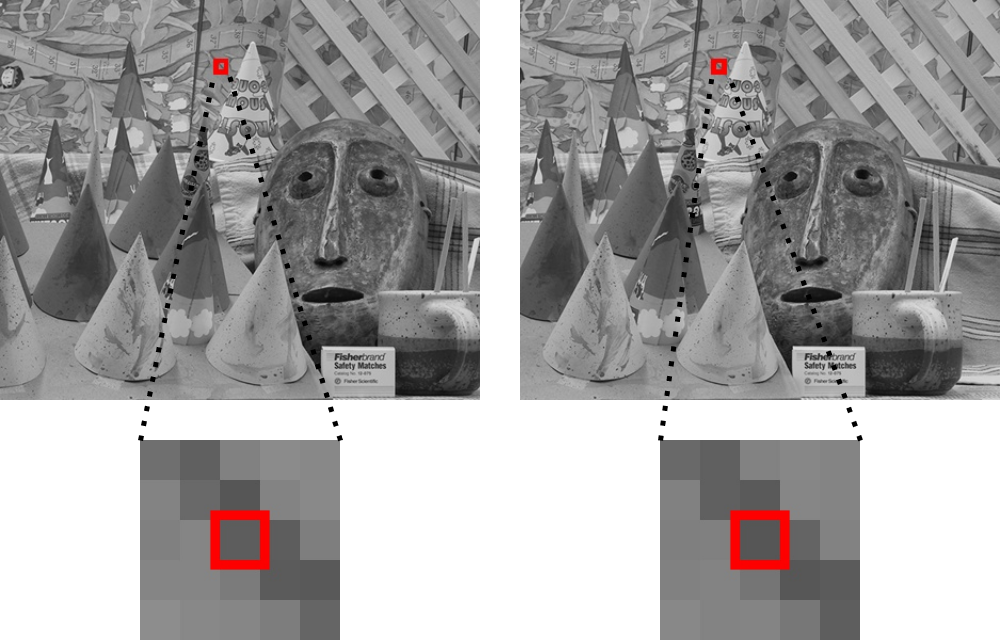
\includegraphics[width=0.8\linewidth]{Images/Cones.png}
  \caption{Homologous pixels in a pair of images}\label{fig:Cones}
\end{figure}

To visualize this uncertainty, we computed upper and lower envelopes for various plausibility levels $\gamma$. These envelopes illustrate the largest (upper bound $\overline{a}$) and smallest (lower bound $\underline{a}$) focal sets where the plausibility, determined by Equation \eqref{eq:bel_pl}, meets or exceeds the given threshold $\gamma$: $\mathrm{Pl}(\overline{a}) \geqslant \gamma$. Consequently, there are two bounds for each level of $\gamma$.
At the plausibility threshold of 0 ($\mathrm{Pl}(\overline{a}) > 0$), the bounds represent the full support of the SAD values. Conversely, at a threshold of 1, the bounds converge to the values of the cost curve obtained in the ``precise'' setting (\ie, without accounting for uncertainty).

\begin{figure}
    \centering
    \begin{subfigure}{0.48\linewidth}
        \centering
        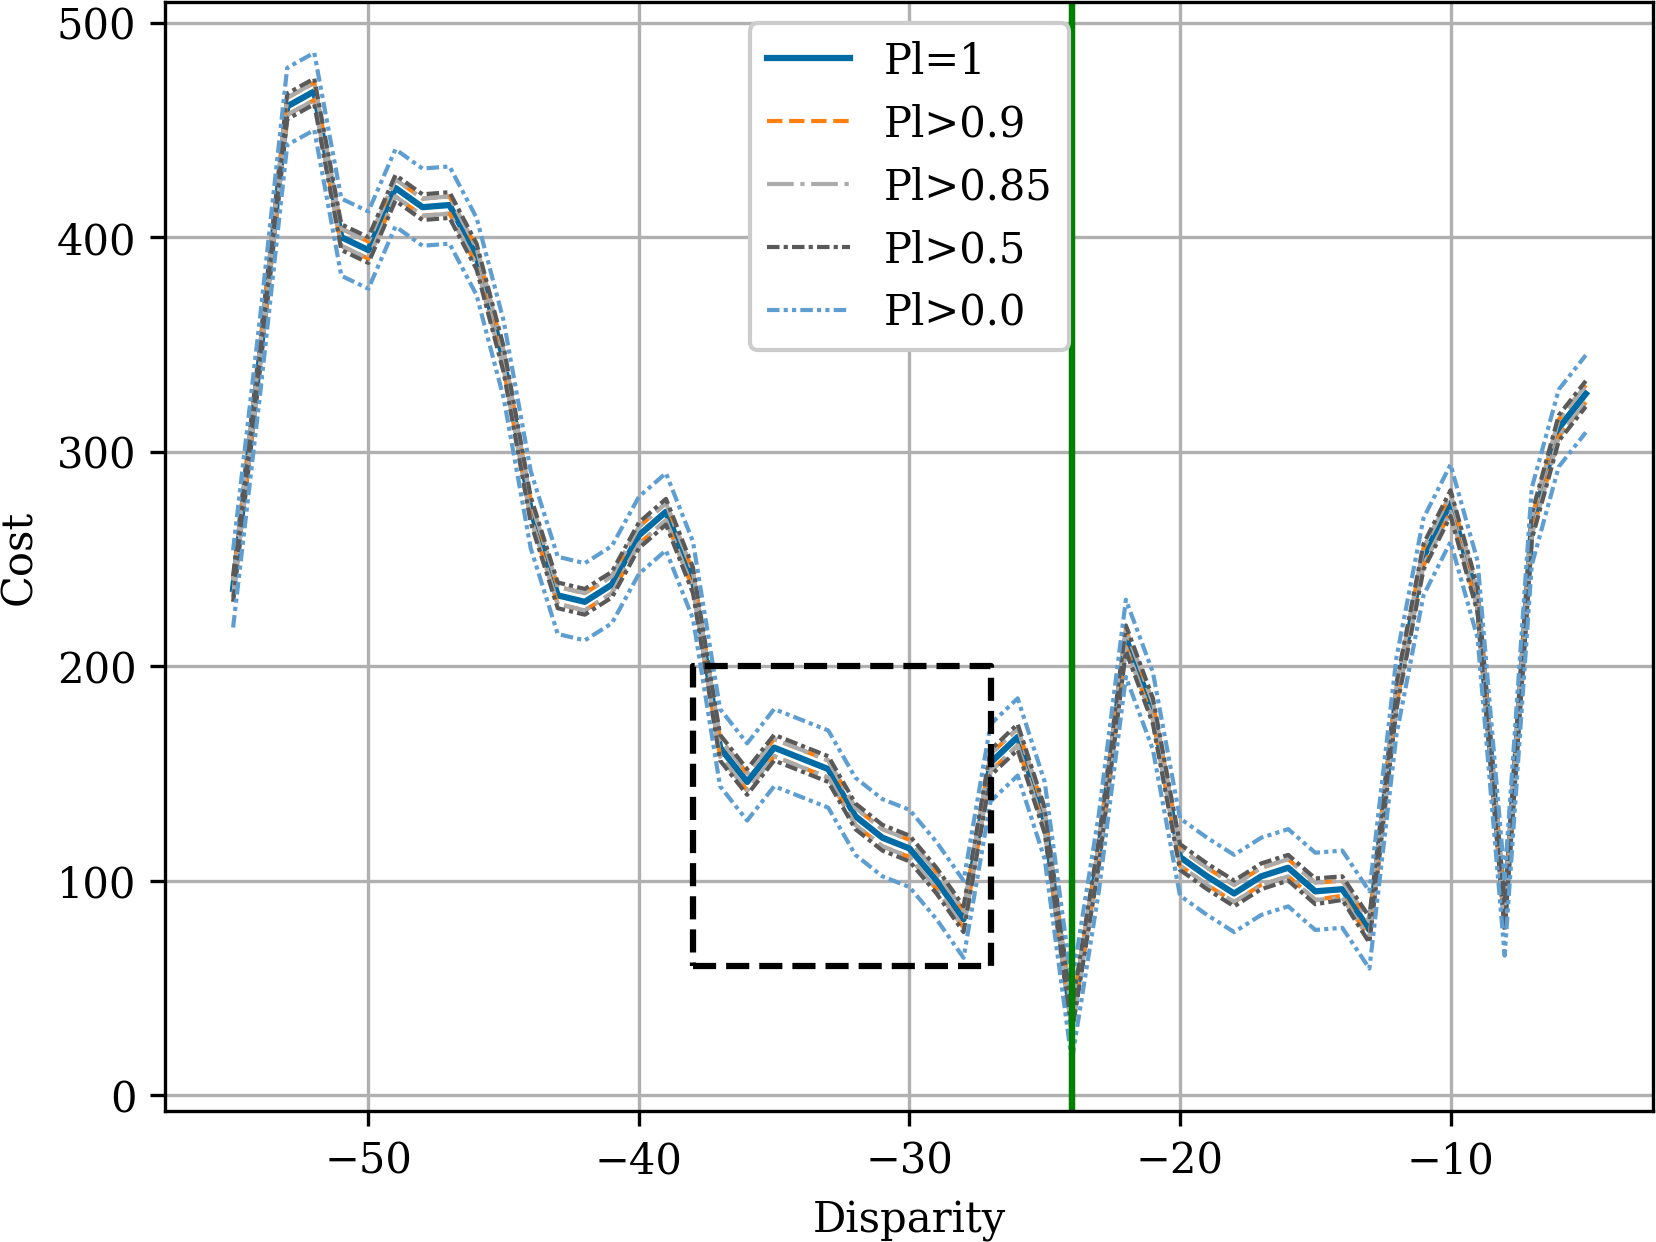
\includegraphics[width=\linewidth]{Images/bel_independence_100_120.png}
        \caption{SAD using the product Copula}
        \label{fig:belief_independence}
    \end{subfigure}\hfill
    \begin{subfigure}{0.48\linewidth}
        \centering
        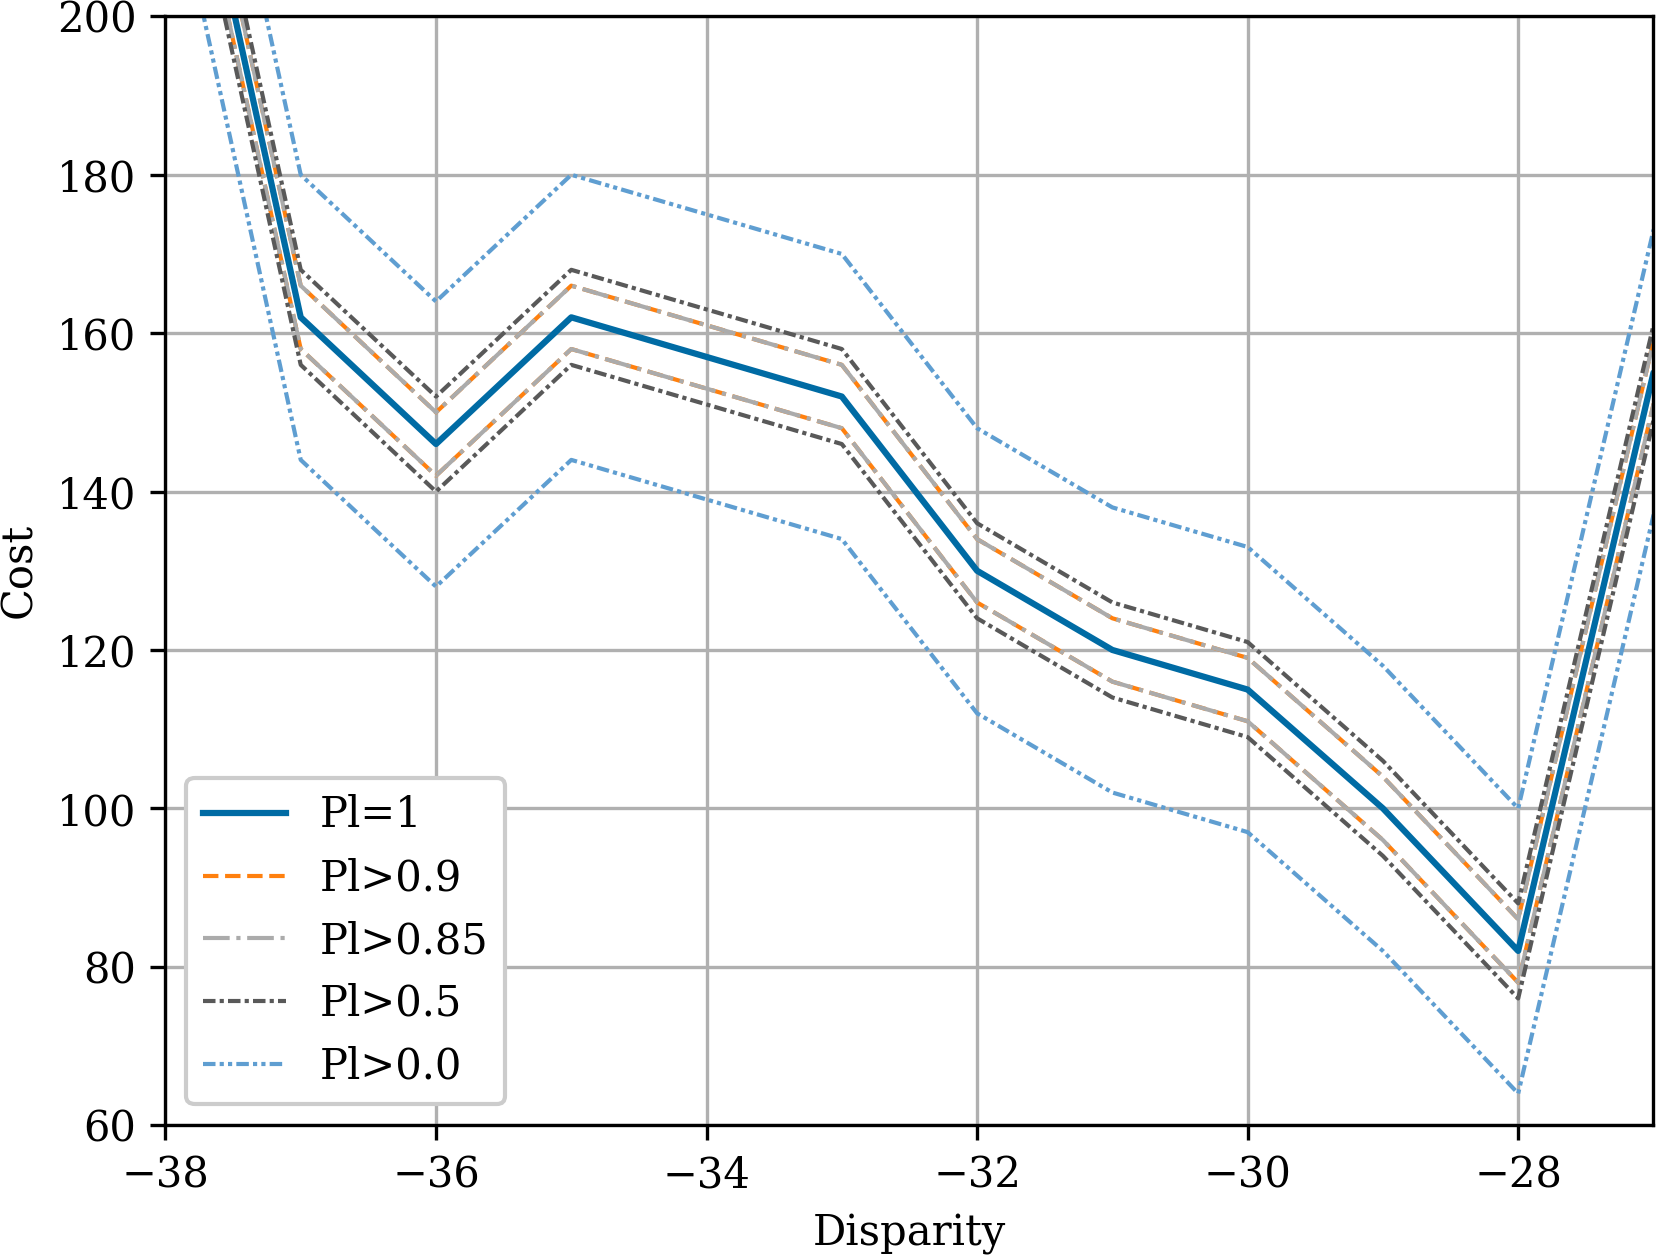
\includegraphics[width=\linewidth]{Images/bel_independence_100_120_zoom.png}
        \caption{Zoom of the rectangle in (a)}
        \label{fig:belief_independence_zoom}
    \end{subfigure}\\
    \begin{subfigure}{0.48\linewidth}
        \centering
        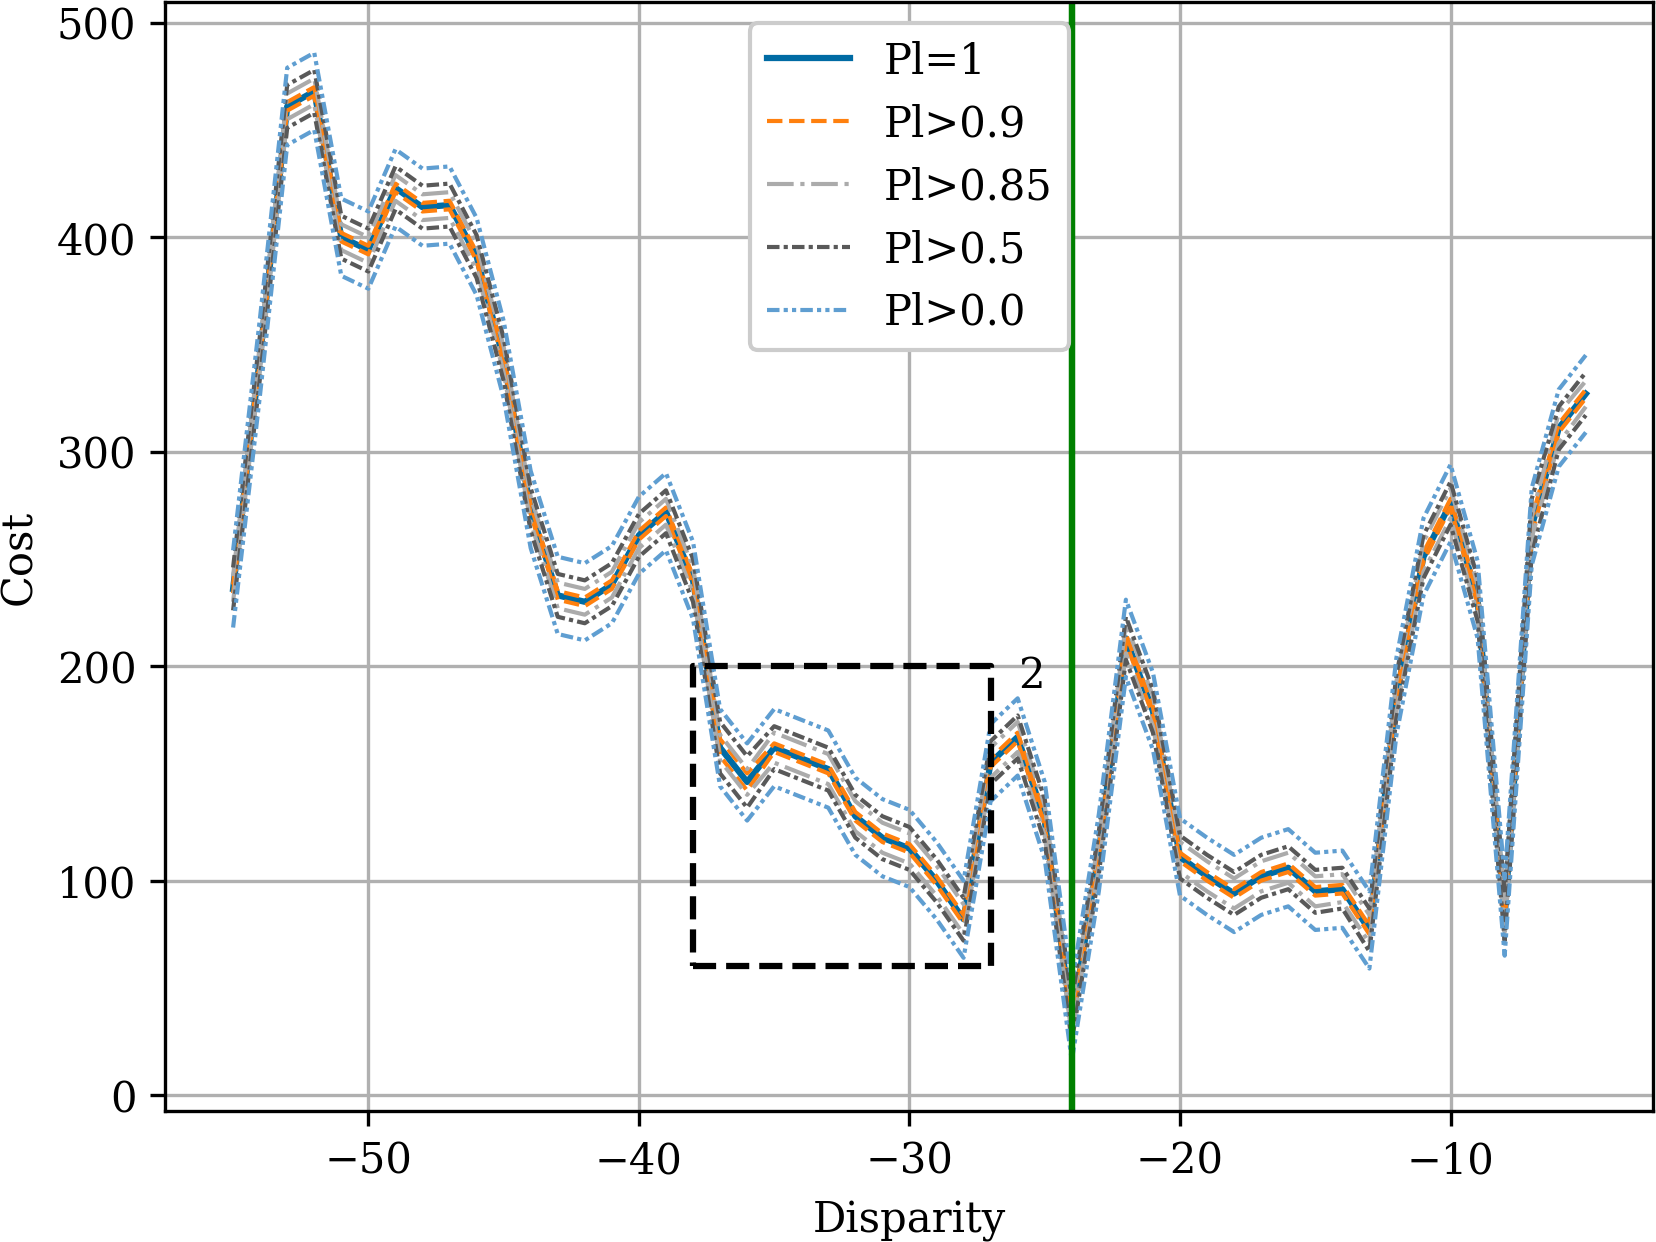
\includegraphics[width=\linewidth]{Images/bel_100_120.png}
        \caption{SAD using the Gaussian Copula}
        \label{fig:belief_gaussian}
    \end{subfigure}\hfill
    \begin{subfigure}{0.48\linewidth}
        \centering
        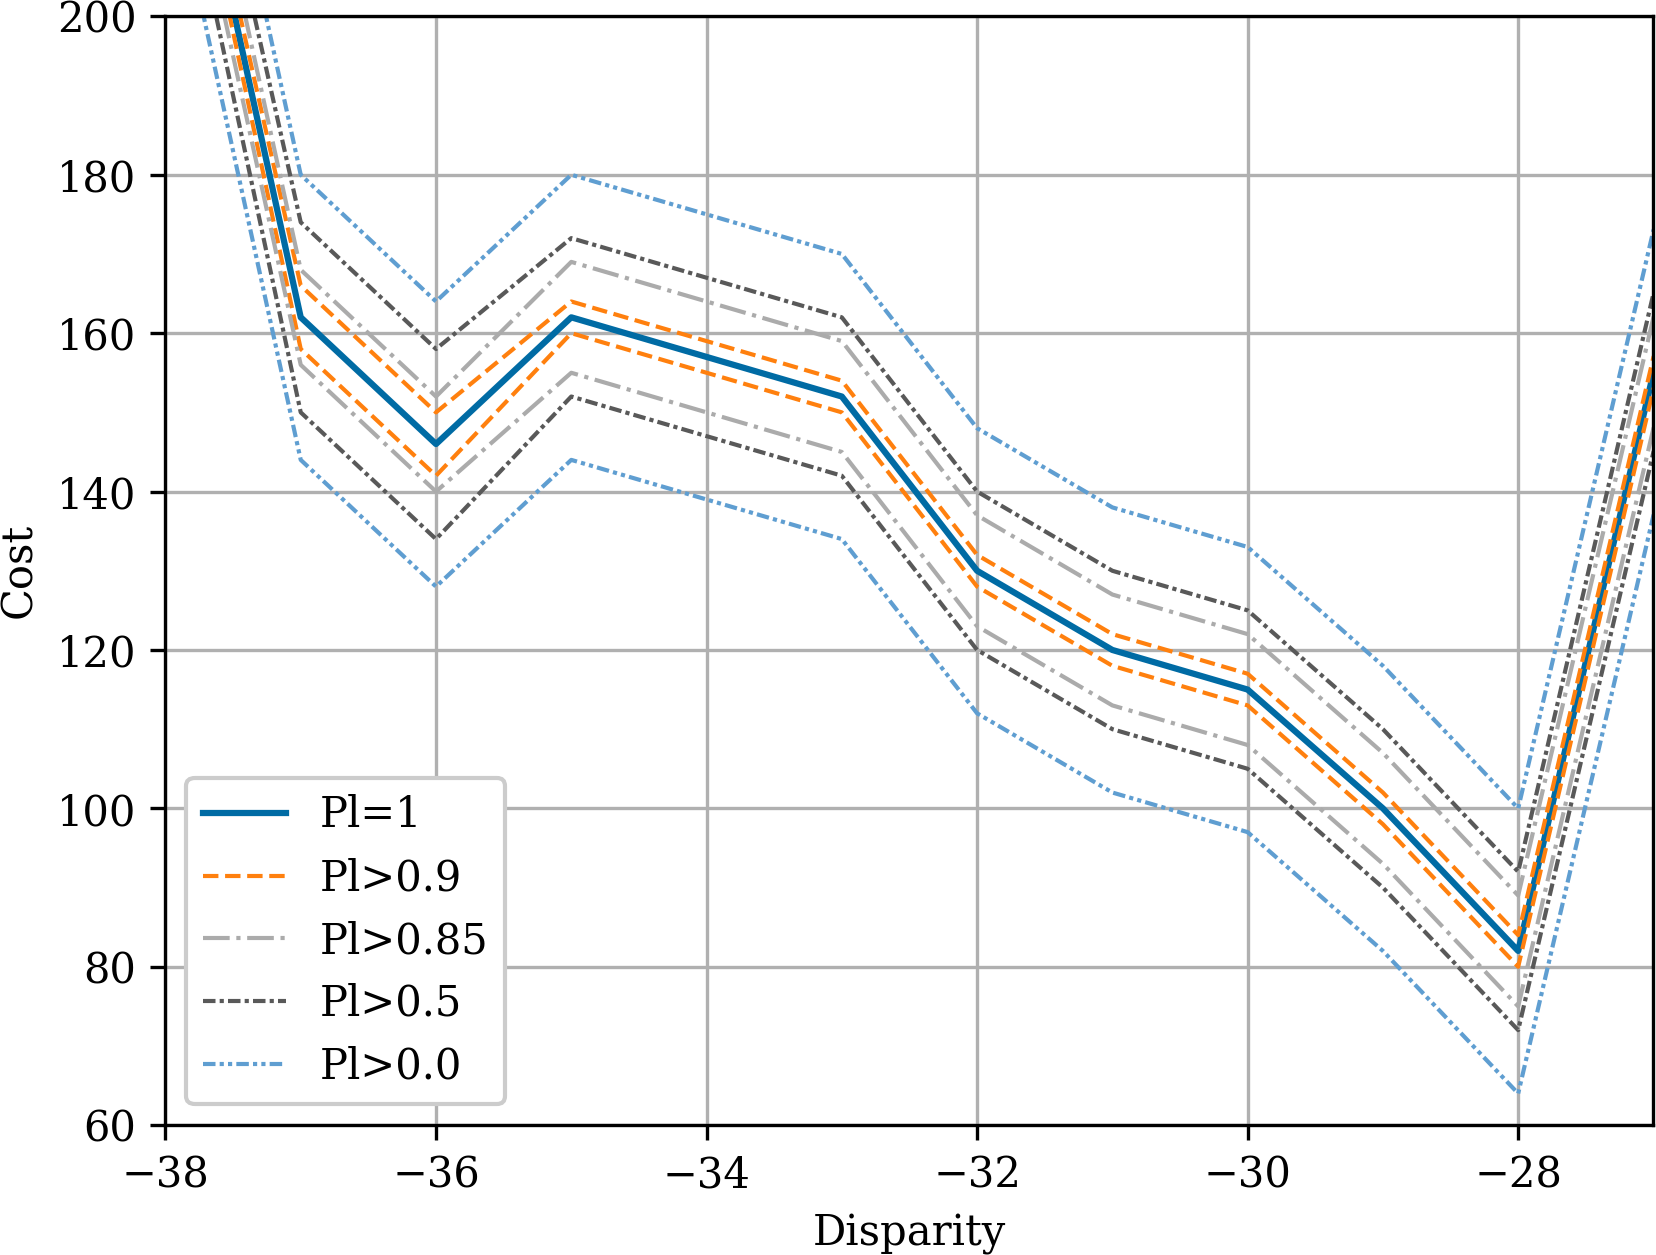
\includegraphics[width=\linewidth]{Images/bel_100_120_zoom.png}
        \caption{Zoom of the rectangle in (c)}
        \label{fig:belief_gaussian_zoom}
    \end{subfigure}
    \caption{Plausibility levels of a cost curve for the product copula $C_\Pi$ and the Gaussian copula $C_R$. The green vertical line represents the true disparity. The figure on the right are a zoom of the black dashed rectangle.}
    \label{fig:belief_curves}
\end{figure}

A visualization of different plausibility levels of the SAD cost curve are presented in figure \ref{fig:belief_curves}, computed with the product copula $C_\Pi$ and a Gaussian copula $C_R$. As both copulas assign non-null masses to the same focal sets, their support ($\mathrm{Pl}>0$) is the same. Taking a copula close to the lower Fréchet-Hoeffding bound (which is not a copula for $n>2$), would lead to a different support, as the image of marginal focal set would be assigned a null mass. Figures \ref{fig:belief_independence_zoom} and \ref{fig:belief_gaussian_zoom} display the fact that the values covered by the plausibility levels vary with the  copula used. The only exception to this concerns the plausibility level $\gamma=1$, corresponding to the SAD curve without noise. The plausibility levels $0.85$ and $0.5$ are more concentrated around plausibility level $1$ in the case of the product copula than in the case of the Gaussian copula. Conversely, plausibility level $0.9$ is closer to plausibility level $1$ in the case of the Gaussian copula. This is due to the fact that the Gaussian copula $C_R$ is more co-monotone than the product copula, given the correlation matrix $R$ described in \eqref{eq:correlation}.

\section{Estimating Propagated Credal Sets Using Monte Carlo Sampling}\label{sec:montecarlo}
In order to evaluate the validity of the propagated belief functions, we try to estimate $\M_{robust}$ using Monte Carlo samplings. We first generate probability distributions belonging in the marginal credal sets. This sampling is not random as we generate probability distributions in such a way that the probability range on events imposed by the marginal possibility distributions is uniformly covered. We also make sure that lower and upper bounds on events are all reached at least once, in order to include ``extreme'' distributions in our simulations. Once every marginal probability distribution of every pixel used to compute a cost curve has been sampled, we can generate random samples from their joint distribution. We thus generate samples from the copula and marginals as detailed in section \ref{sec:sampling_copula}. This yields noised version of patches from the left images, where the noised samples dependency is modeled by the provided copula. Finally, we compute the cost curves using those random images, giving us Monte Carlo samples of the SAD cost curves for a given copula.

Note that we could simulate a single version of the noised pair of images, but that would require to sample from a copula of very large dimension (the number of pixels in both images). This is not realistically feasible, even thought it would ensure that the same version of noised pixels are used in all cost curves (or in other words, for a single draw, the noised intensities will not change depending on the cost curve computed). We instead generate noise samples for each row separately: noised values of pixels will not change during the evaluation of a cost curve for different disparities, or between the cost curves of pixels of the same row. However, their values might change between cost curves of pixels belonging to different rows. For instance, let's consider a pixel $p=(row,~col)\in I_L$ for which we computed a noised intensity $i_p$. Then we will use the same noised value $i_p$ of intensity when computing the SAD of every pixel $q=(row,~col')\in I_L$. But when computing the SAD of every pixel $q=(row-1,~col')\in I_L$, we will use a different Monte Carlo draw for the value $i_p$, which will stay the same for every pixel of row $row-1$. Because we draw a high number of Monte Carlo draws ($10,000$) for each row, the effect of this of proceeding should not be noticeable. 

Monte Carlo draws using the Gaussian copula and marginals credal sets of \ref{eq:pixel_possibility} are plotted in figures \ref{fig:montecarlo_gauss_100_120} and \ref{fig:montecarlo_gauss_200_150}. Different plausibility levels, similar to those of figures \ref{fig:belief_curves}, also appear for comparison. The support envelopes from plausibility levels $\mathrm{Pl}>0$ correctly contain all Monte Carlo samplings for all considered copulas. We can observe in Figure \ref{fig:montecarlo_gauss_200_150_zoom2} that plausibility levels sometimes fail to correctly grasp the fluctuations of the dispersion of the samples, even though they seem to correctly contain Monte Carlo samples. For instance, Monte Carlo draws are first dense around disparity $-37$, then seem to spread around $-35$, and finally regather around disparity $-32$. The plausibility envelopes are more regular in this disparity range. This illustrates the fact the ``true'' point-wise credal $\M_{robust}$ set described in section \ref{sec:robust_method} and approximated with Monte Carlo samples is different from that the joint credal set $\M_{mass}$ from section \ref{sec:joint_mass}. Although some differences persist between those sets, Figure \ref{fig:montecarlo_gauss_100_120_zoom2} or \ref{fig:montecarlo_gauss_200_150_zoom2} suggest that Monte Carlo simulations can correctly estimate the point-wise credal set $\M_{robust}$ by joining belief functions using a copula as in equation \eqref{eq:joint_mass}. This is furthermore justified by the  quantitative analysis presented in Table \ref{tab:Coverage}, where the proportion of Monte Carlo samplings contained inside the plausibility envelopes, is computed for different plausibility levels $\gamma$. We will call this proportion ``coverage''. The coverage for figures \ref{fig:montecarlo_gauss_100_120} and \ref{fig:montecarlo_gauss_200_150} are presented in the first and second rows of Table \ref{tab:Coverage} respectively. The global coverage over the whole left image is presented in the last row of the table. The coverage is always $100\%$ for $\gamma=0$, which indicates that every sample is contained inside the support envelopes. \todoroman{Je pense que ce que je dis ensuite est faux. Le coverage ne donne pas d'indication sur les plausibility estimées, car celles ci ne retranscrivent pas une fréquence mais seulement un niveau de croyance. Comment donner une interprétation correcte de la densité?} As envelopes are defined as lower and upper bounds of the focal sets with a plausibility superior to $\gamma$, the coverage should be superior to $1-\gamma$, which is indeed the case.

\begin{figure}
    \centering
    \begin{subfigure}{1\linewidth}
        \centering
        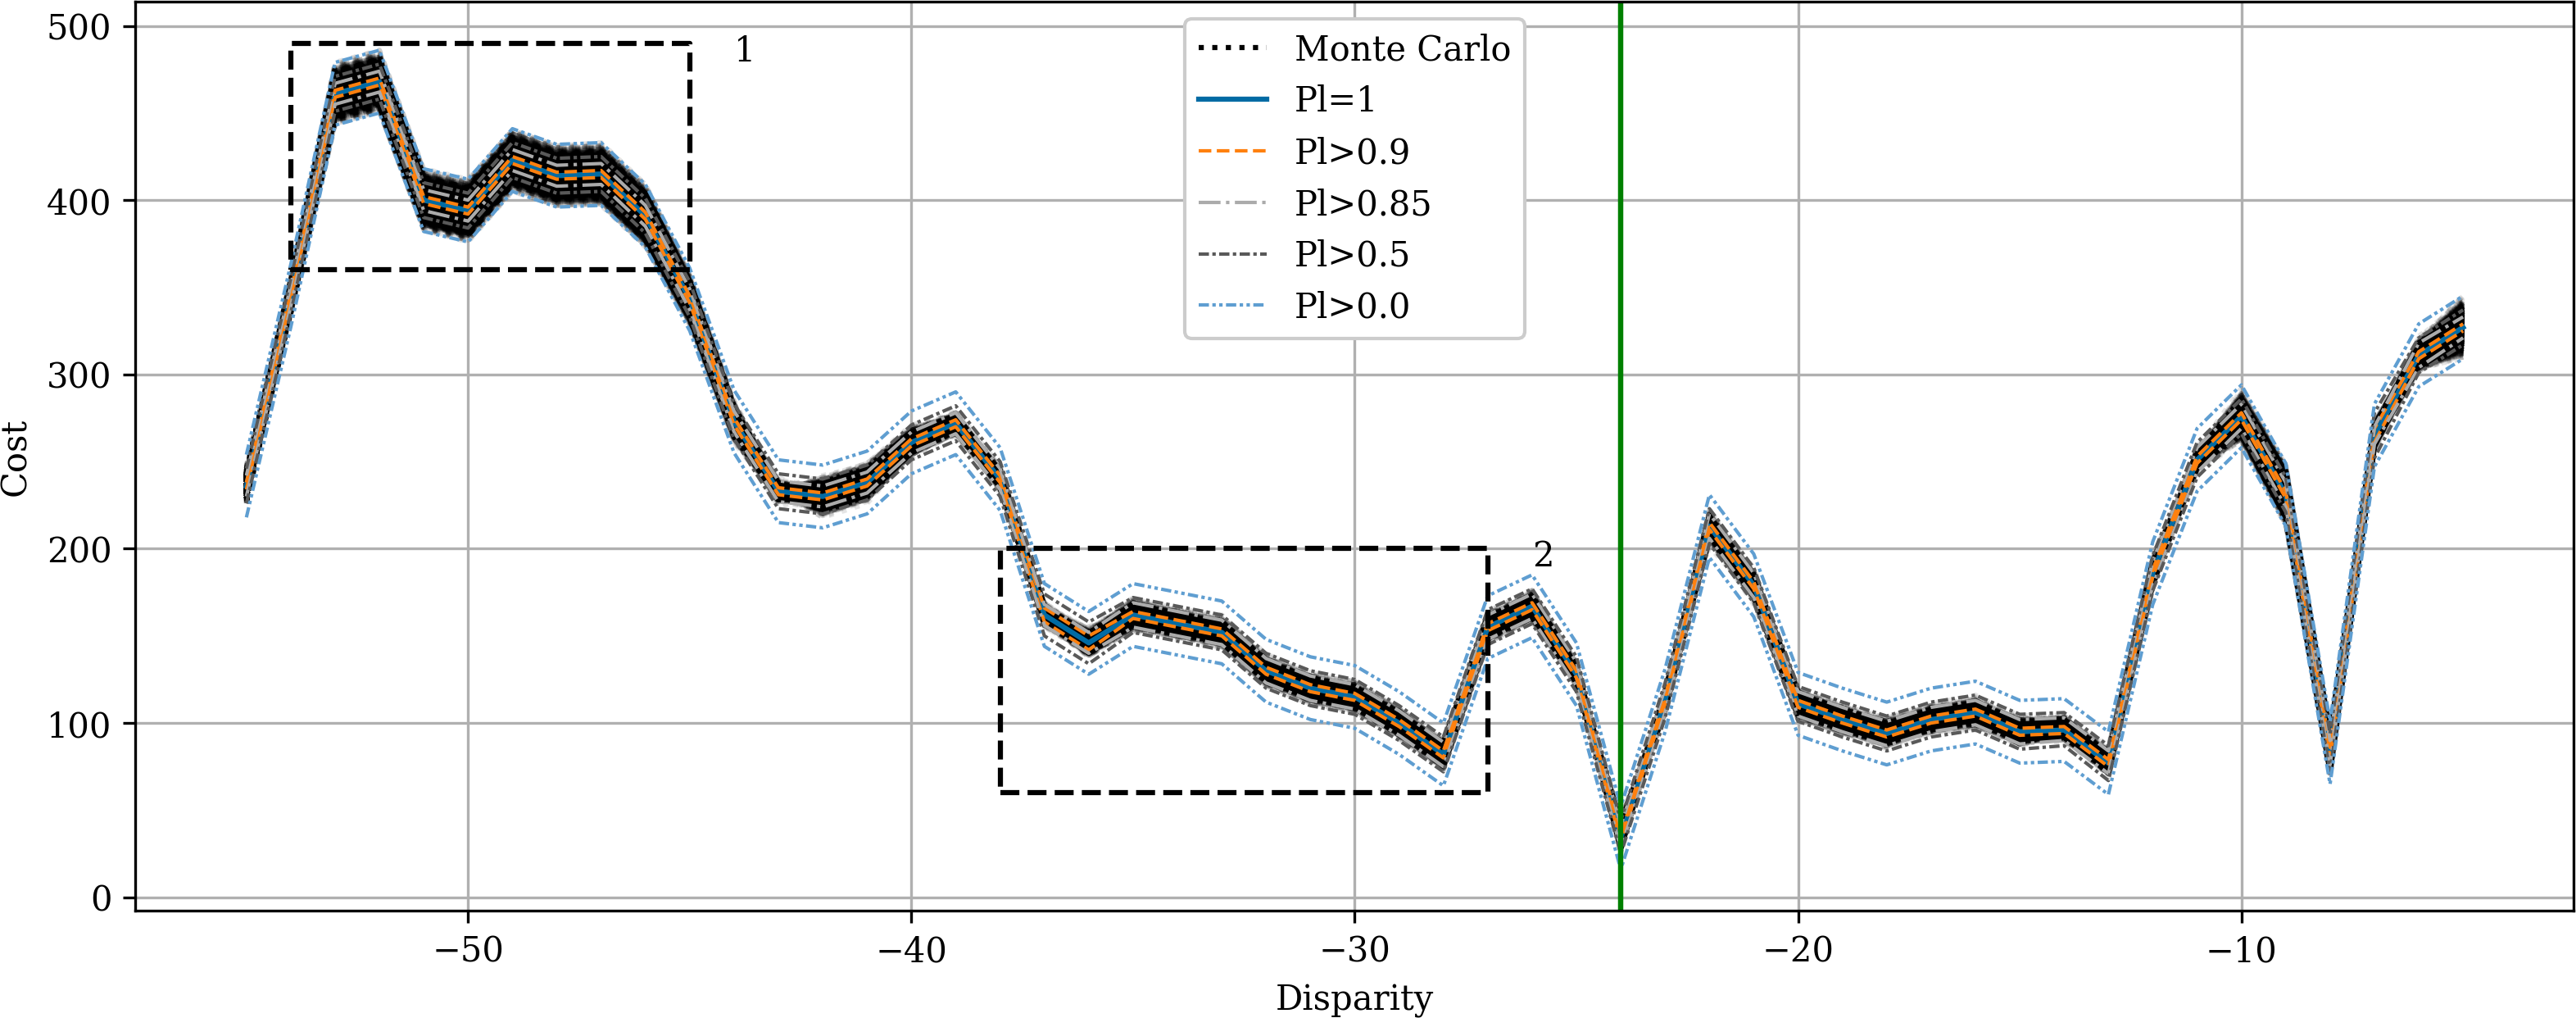
\includegraphics[width=\linewidth]{Images/cost_curve_100_120.png}
        \caption{Plausibility levels and Monte Carlo sampling using a Gaussian copula}
        \label{fig:montecarlo_gauss_100_120_large}
    \end{subfigure}\\
    \begin{subfigure}{0.45\linewidth}
        \centering
        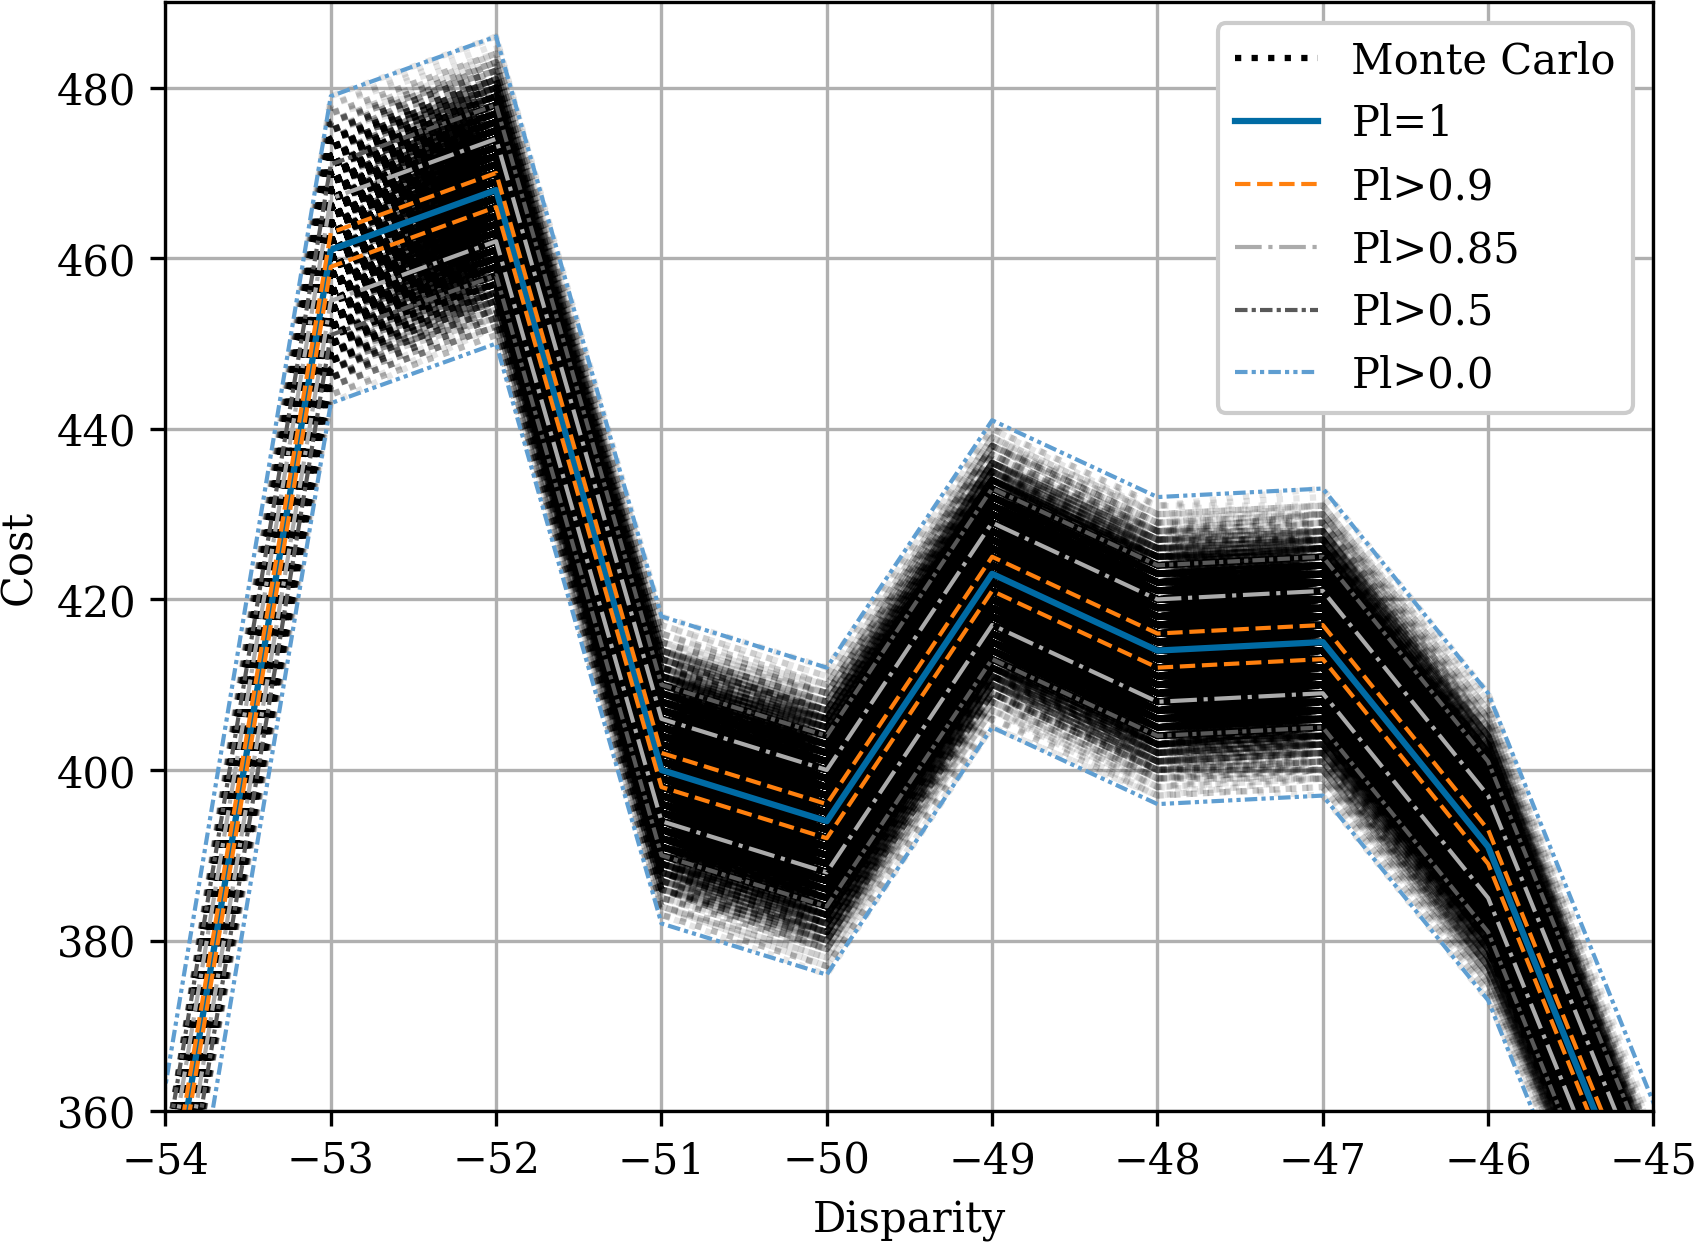
\includegraphics[width=\linewidth]{Images/cost_curve_100_120_zoom1.png}
        \caption{Zoom over the first rectangle}
        \label{fig:montecarlo_gauss_100_120_zoom1}
    \end{subfigure}\hfill
    \begin{subfigure}{0.45\linewidth}
        \centering
        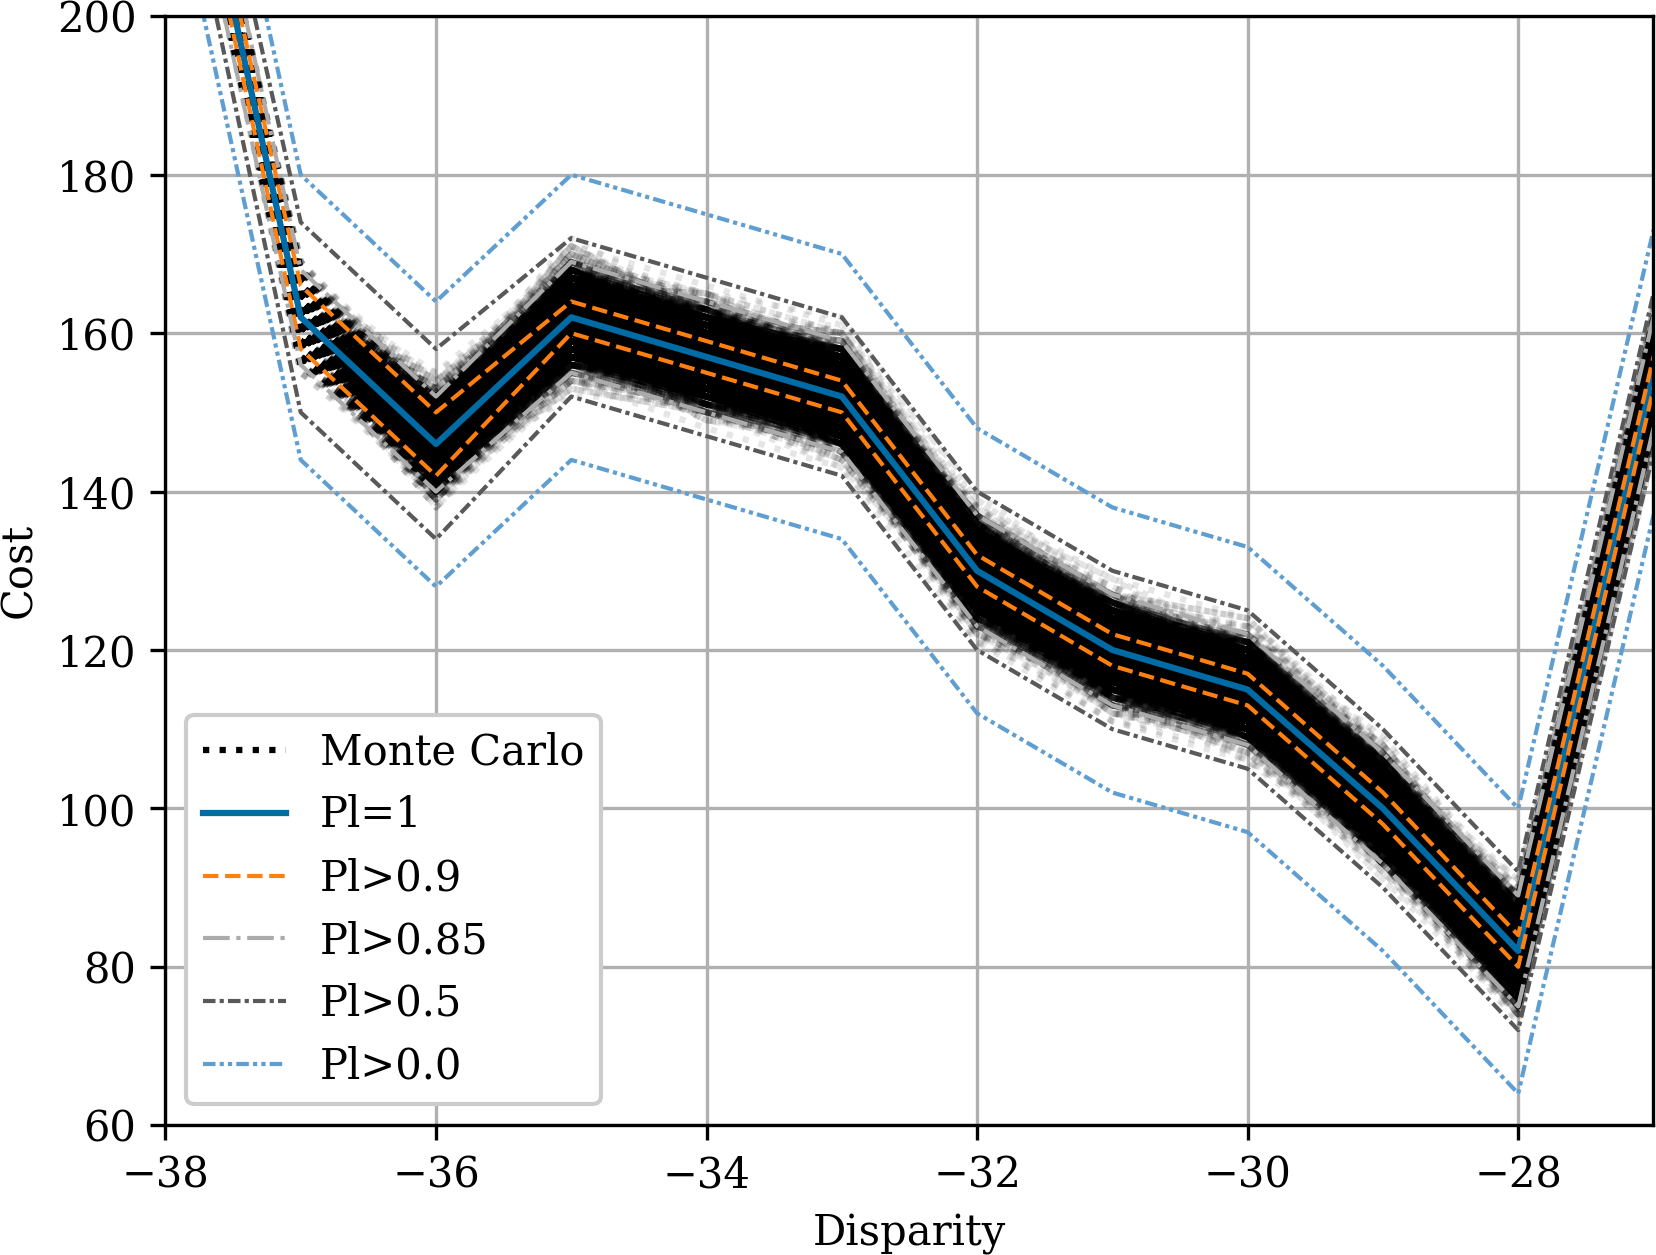
\includegraphics[width=\linewidth]{Images/cost_curve_100_120_zoom2.png}
        \caption{Zoom over the second rectangle}
        \label{fig:montecarlo_gauss_100_120_zoom2}
    \end{subfigure}
    \caption{Plausibility levels and Monte Carlo sampling for a pixel of the left image}
    \label{fig:montecarlo_gauss_100_120}
\end{figure}

\begin{figure}
    \centering
    \begin{subfigure}{\linewidth}
        \centering
        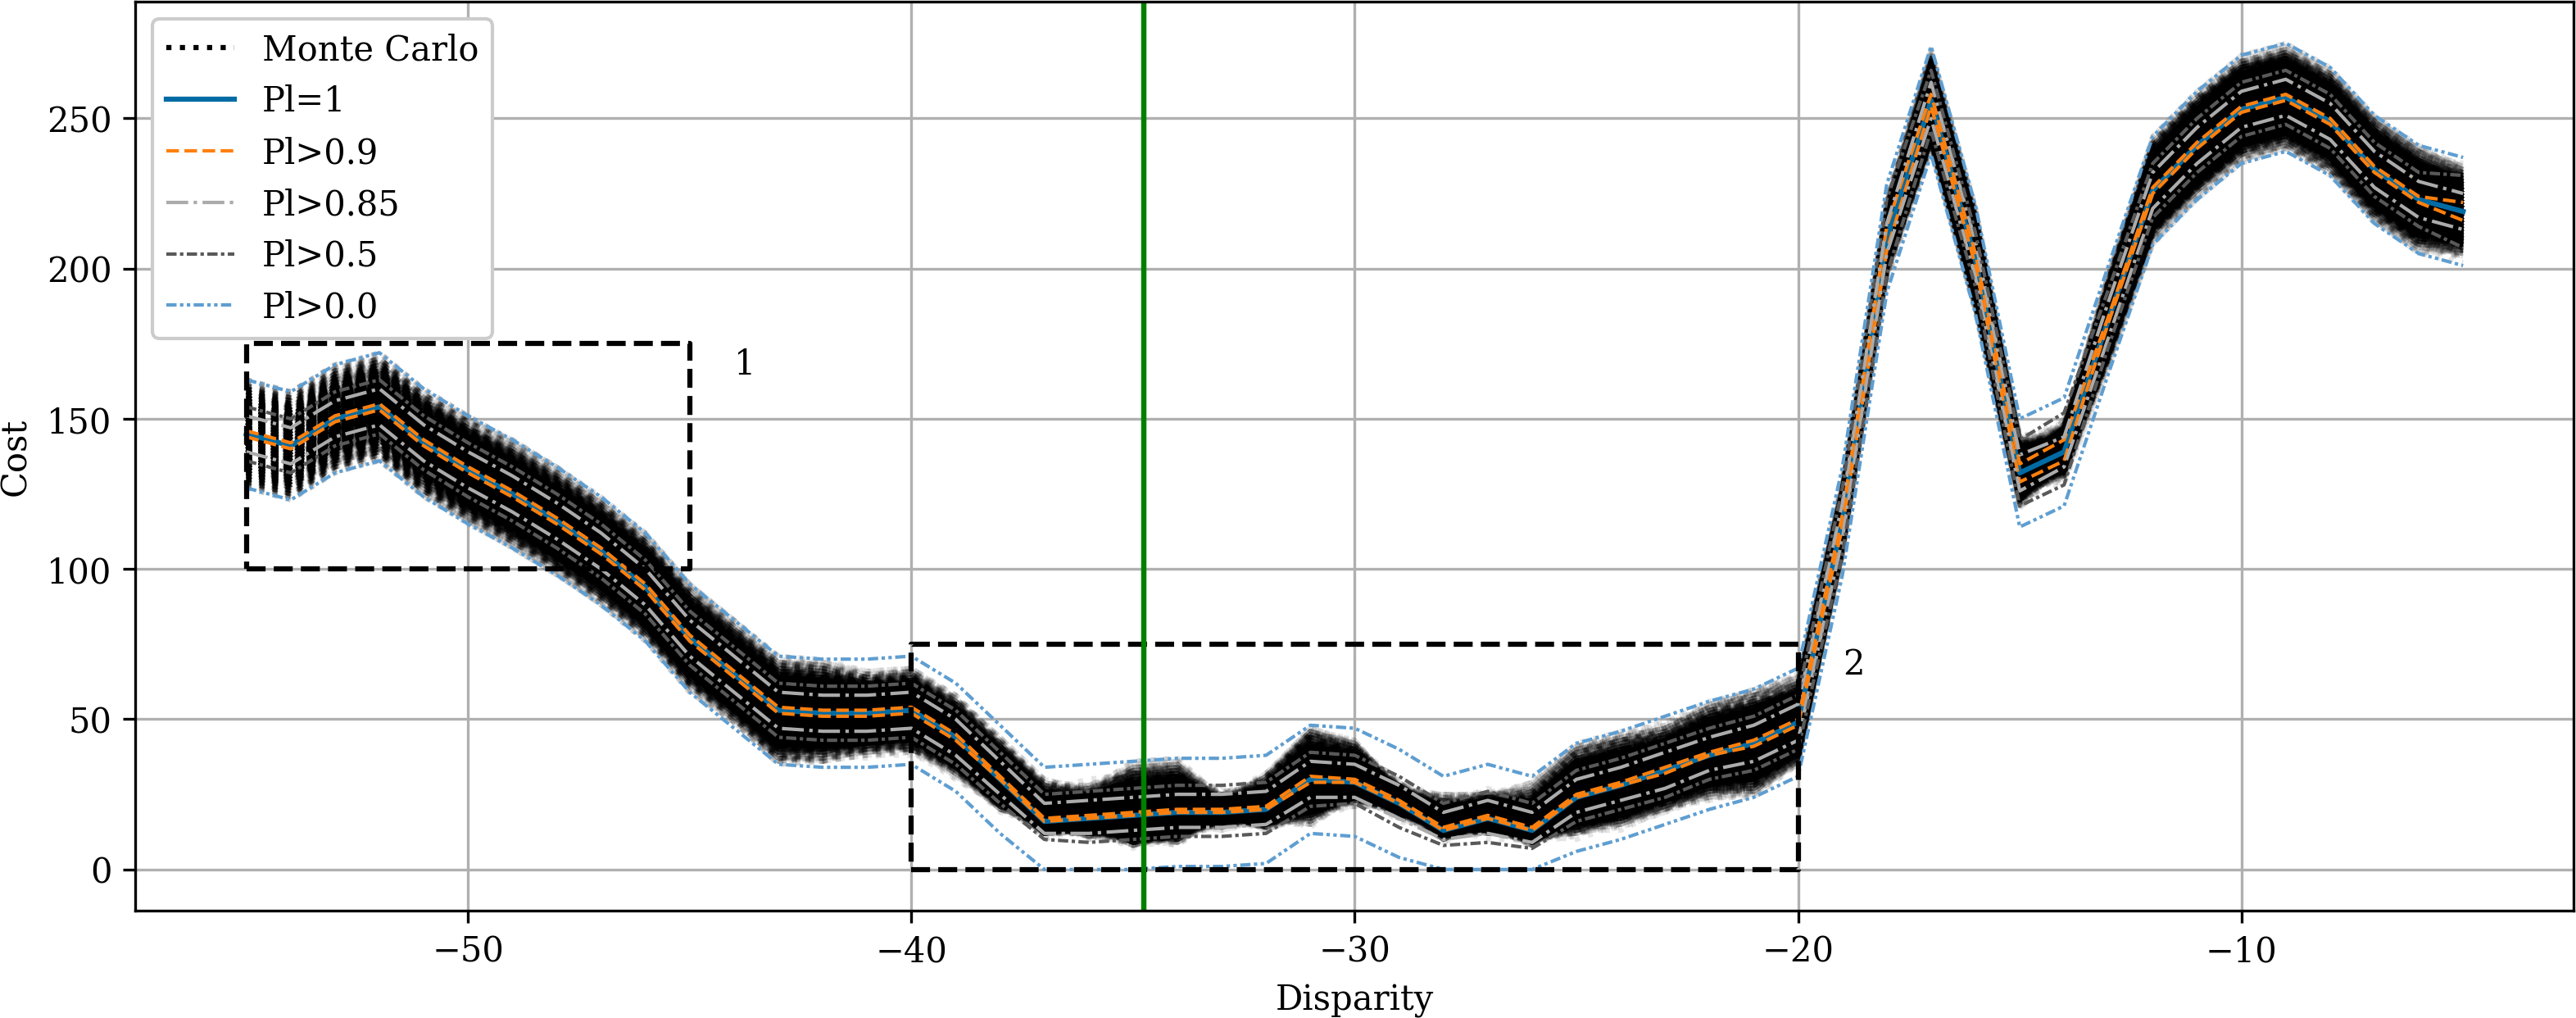
\includegraphics[width=\linewidth]{Images/cost_curve_200_150.png}
        \caption{Plausibility levels and Monte Carlo sampling using a Gaussian copula}
        \label{fig:montecarlo_gauss_200_150_large}
    \end{subfigure}\\
    \begin{subfigure}{0.45\linewidth}
        \centering
        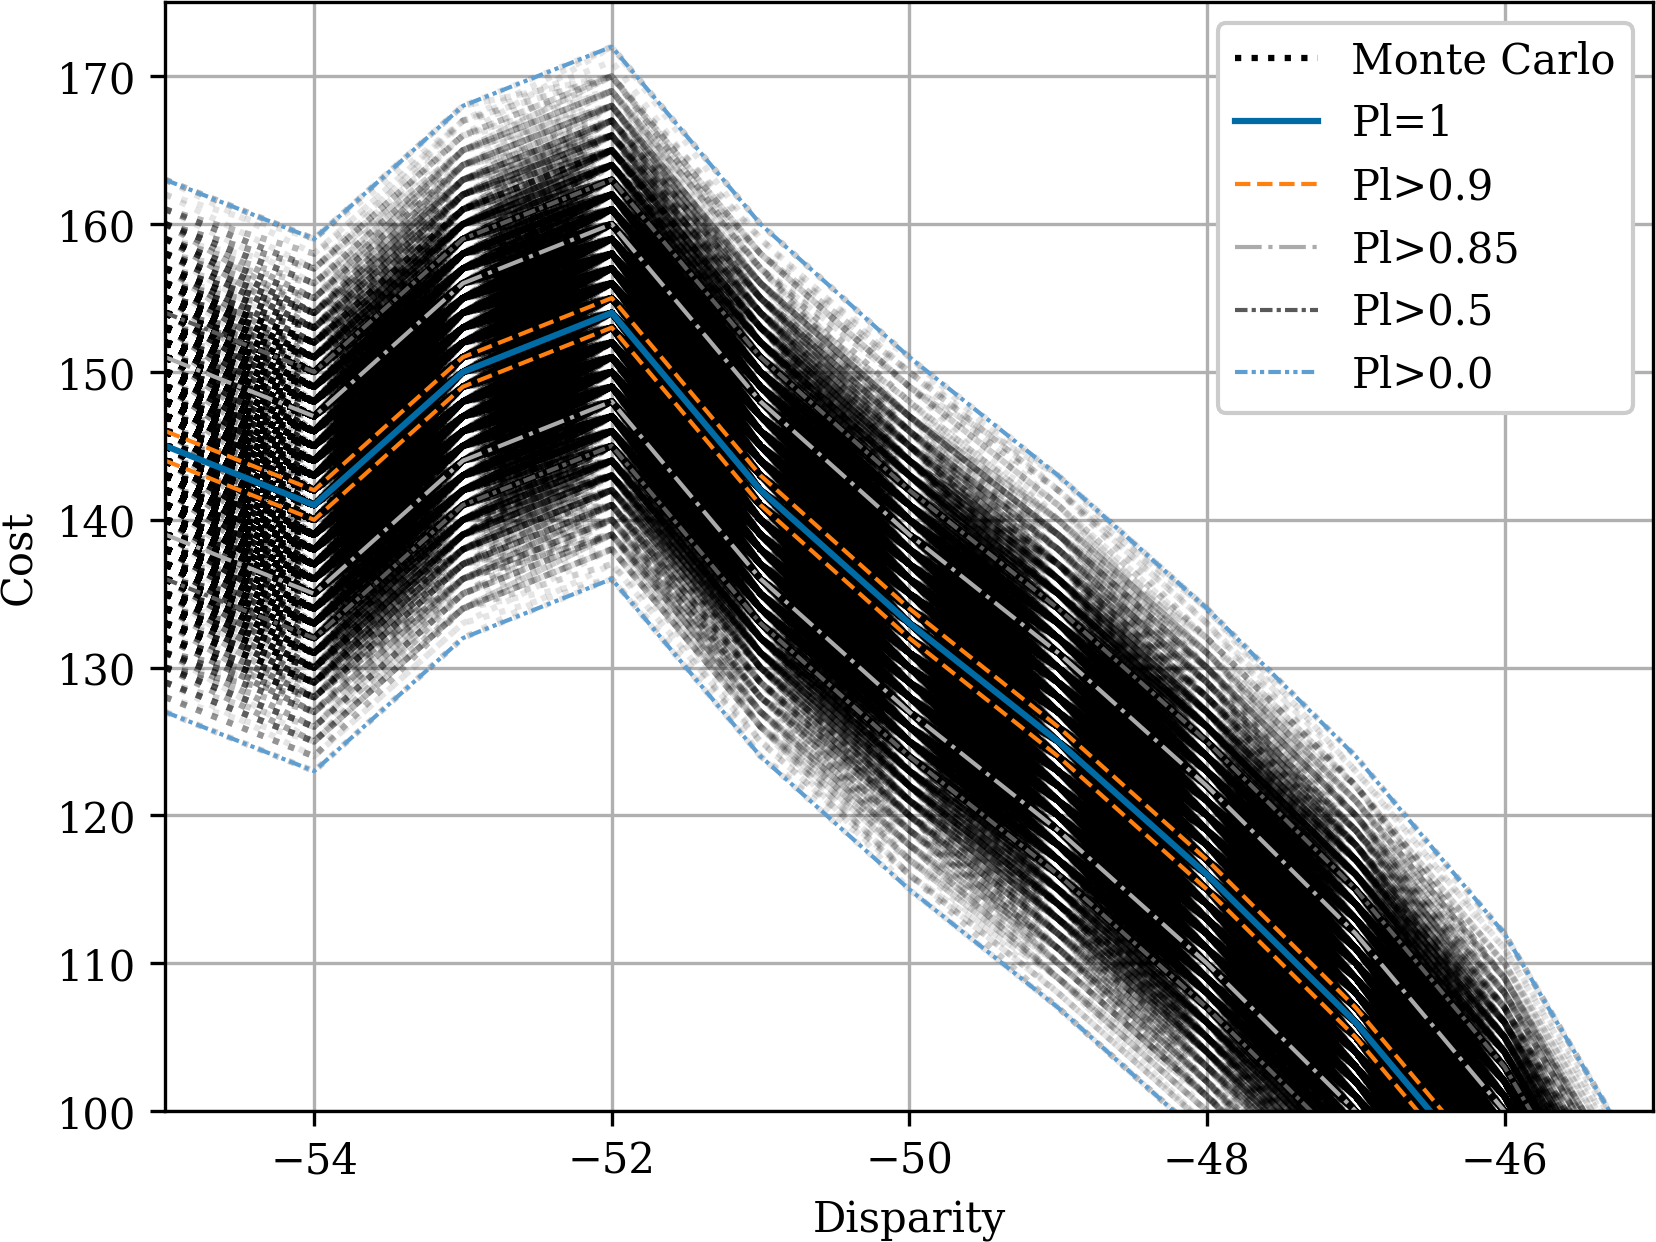
\includegraphics[width=\linewidth]{Images/cost_curve_200_150_zoom1.png}
        \caption{Zoom over the first rectangle}
        \label{fig:montecarlo_gauss_200_150_zoom1}
    \end{subfigure}
    \hfill
    \begin{subfigure}{0.45\linewidth}
        \centering
        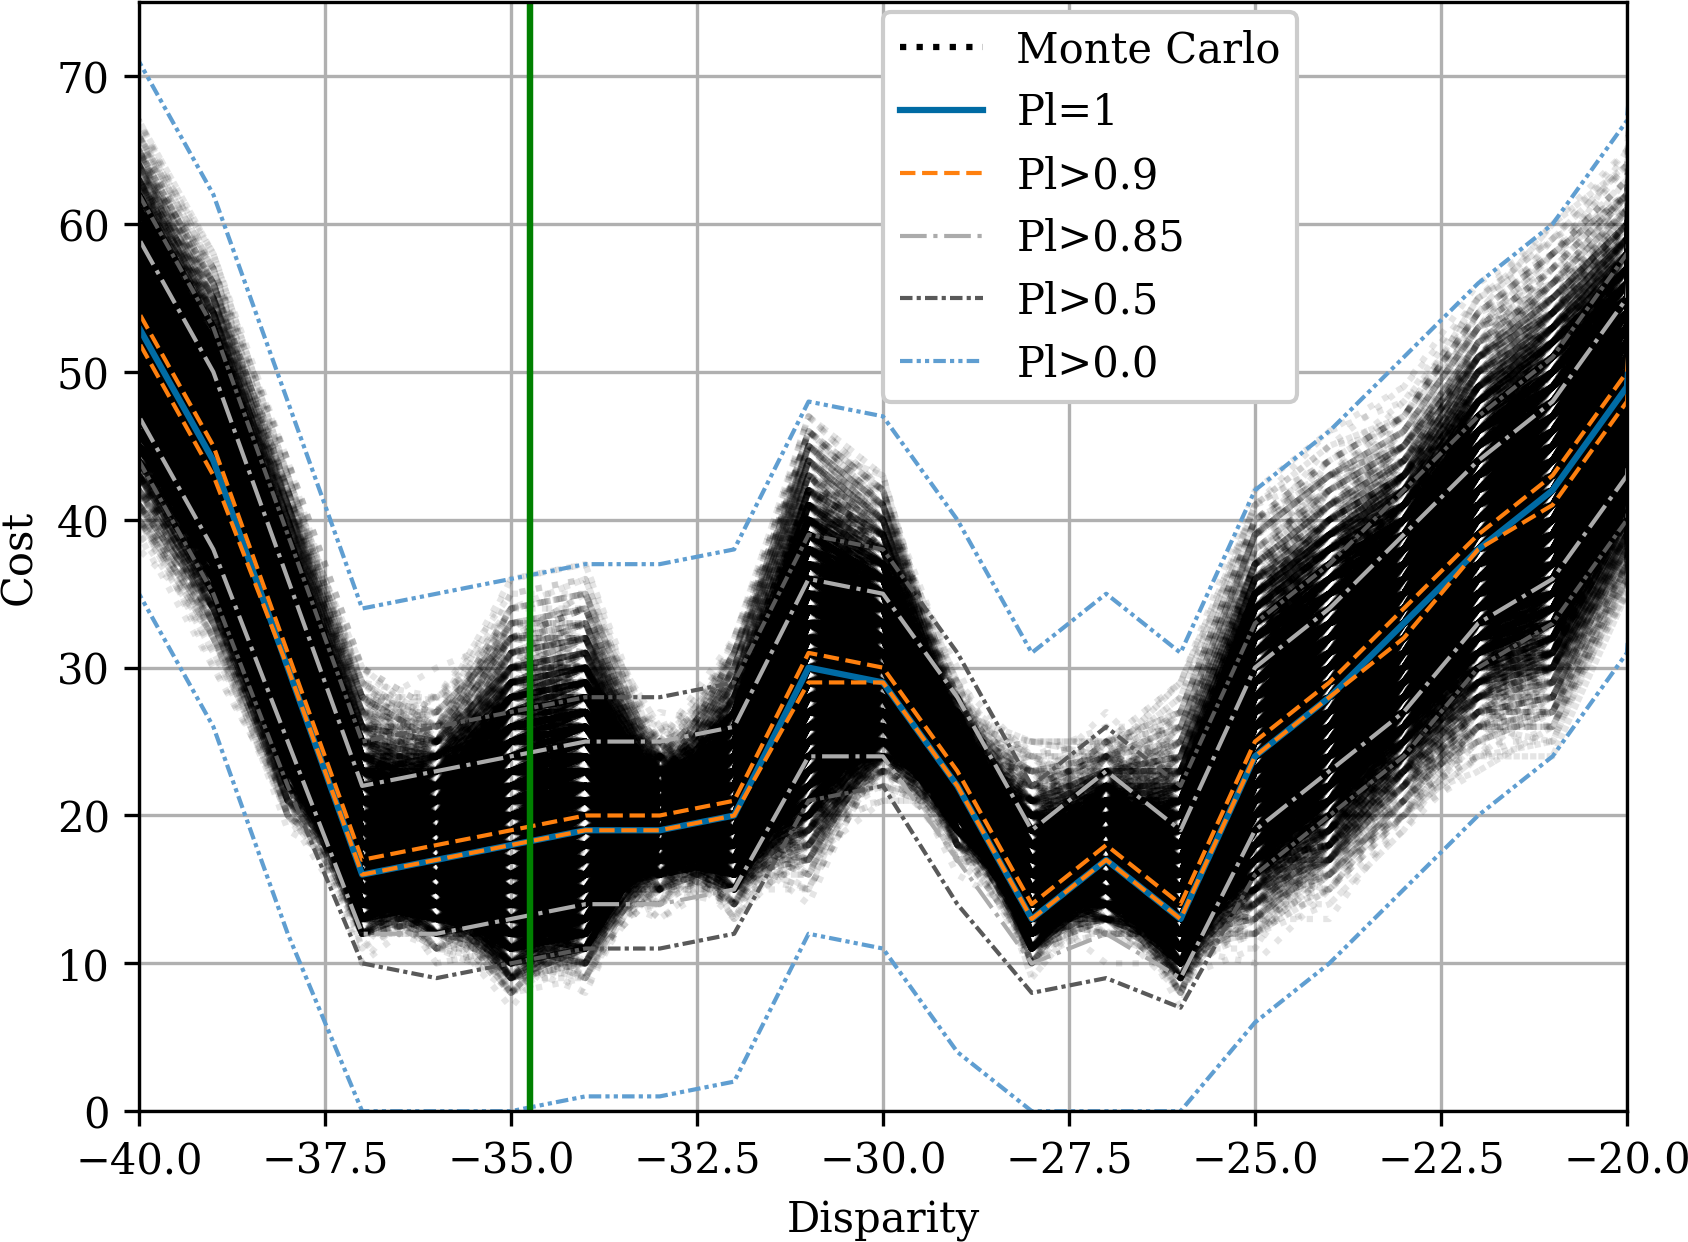
\includegraphics[width=\linewidth]{Images/cost_curve_200_150_zoom2.png}
        \caption{Zoom over the second rectangle}
        \label{fig:montecarlo_gauss_200_150_zoom2}
    \end{subfigure}
    \caption{Plausibility levels and Monte Carlo sampling for a pixel of the left image}
    \label{fig:montecarlo_gauss_200_150}
\end{figure}

\begin{table}[ht]
\centering
\begin{tabular}{|c|c|c|c|c|}
\hline
\rowcolor[HTML]{C0C0C0}
$p=(row,col)$ & $\gamma=0.9$  & $\gamma=0.85$ & $\gamma=0.5$  & $\gamma=0$   \\ \hline
\cellcolor[HTML]{C0C0C0}$(100,~120)$     & $64,5\%$ & $94,5\%$ & $99,0\%$ & $100\%$ \\ \hline
\cellcolor[HTML]{C0C0C0}$(200,~150)$     & $30,0\%$ & $82,6\%$ & $95,2\%$ & $100\%$ \\ \hline
\cellcolor[HTML]{C0C0C0}Global        & $41,1\%$ & $87,6\%$ & $96,8\%$ & $100\%$ \\ \hline
\end{tabular}
\caption{Average coverage for various plausibility levels $\gamma$ and for different pixels $p$ of the left image.}\label{tab:Coverage}
\end{table}

\begin{figure}[ht]
    \centering
    \begin{subfigure}{0.48\linewidth}
        \centering
        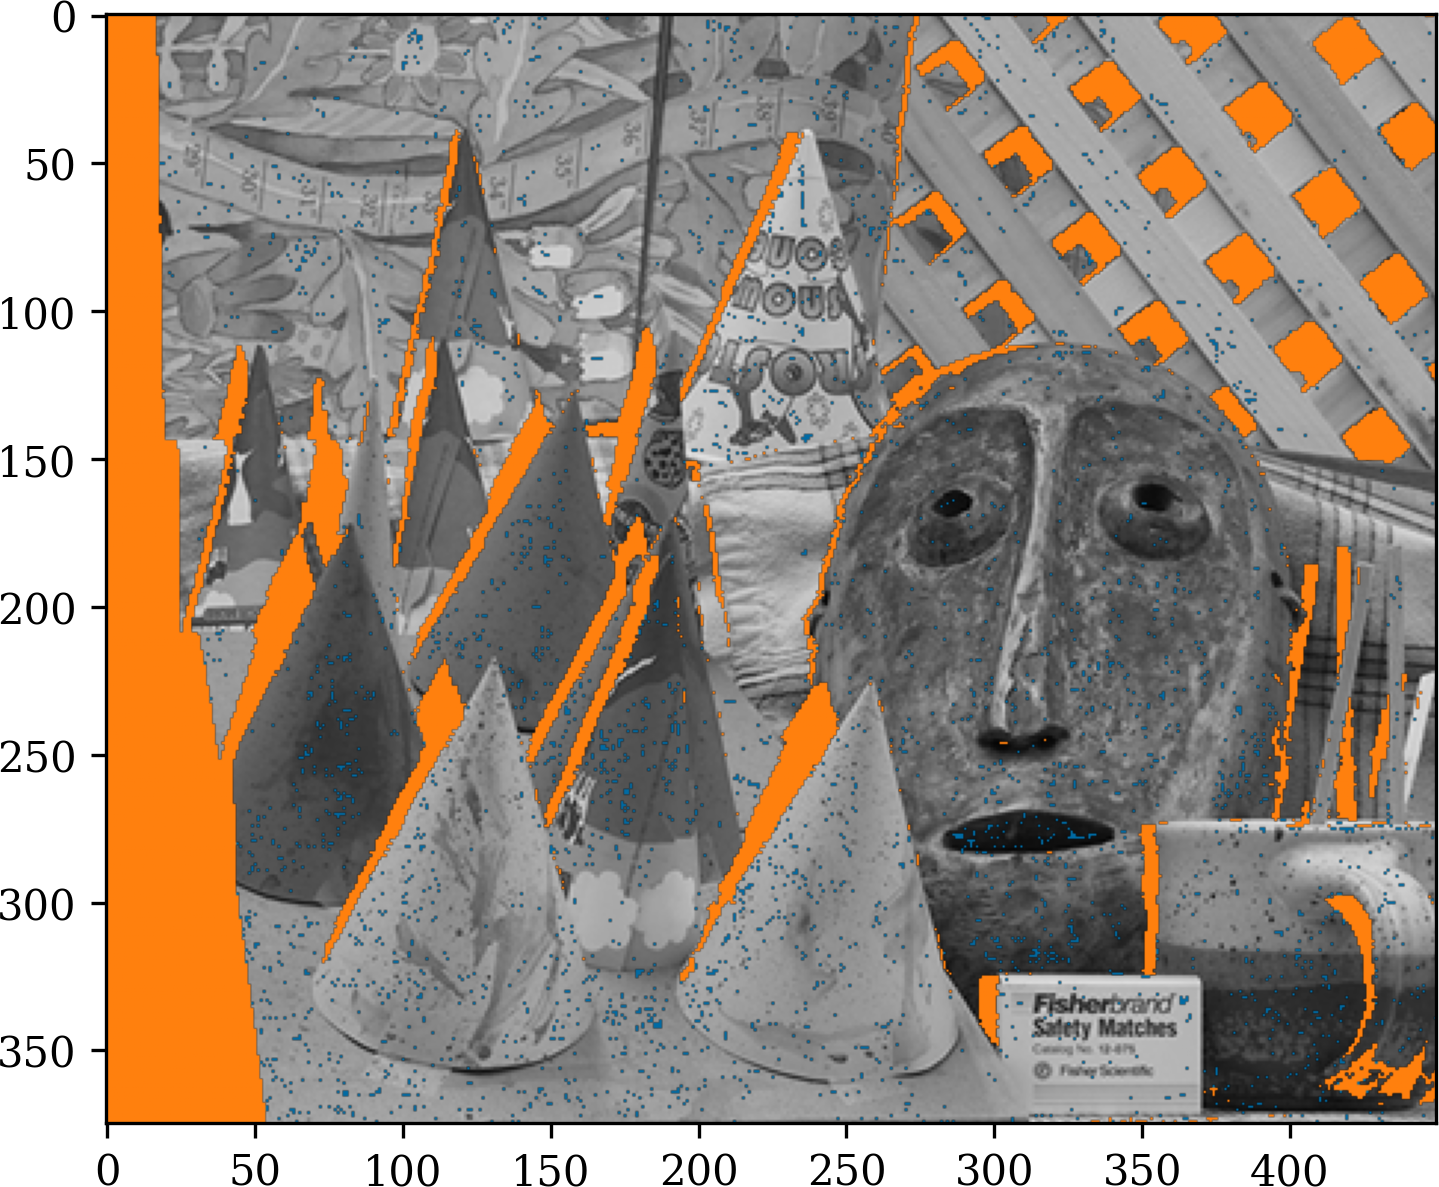
\includegraphics[width=\linewidth]{Images/Improvements_Pl=0.9.png}
        \caption{$\gamma=0.9,~\Delta s_\gamma=4.05\%$}
        \label{fig:improvements_a}
    \end{subfigure}
    \begin{subfigure}{0.48\linewidth}
        \centering
        \includegraphics[width=\linewidth]{Images/Improvements_Pl=0.85.png}
        \caption{$\gamma=0.85,~\Delta s_\gamma=16.11\%$}
        \label{fig:improvements_b}
    \end{subfigure}\\
    \begin{subfigure}{0.48\linewidth}
        \centering
        \includegraphics[width=\linewidth]{Images/Improvements_Pl=0.5.png}
        \caption{$\gamma=0.5,~\Delta s_\gamma=21.41\%$}
        \label{fig:improvements_c}
    \end{subfigure}
    \begin{subfigure}{0.48\linewidth}
        \centering
        \includegraphics[width=\linewidth]{Images/Improvements_Pl=0.0.png}
        \caption{$\gamma=0,~\Delta s_\gamma=28.87\%$}
        \label{fig:improvements_d}
    \end{subfigure}
    \caption{Spatial disposition of potential improvements for different values of $\gamma$. Pixels with potential improvements appear in blue. Occluded pixels, for which a correct disparity does not exist, appear in orange. Grayscale left image is displayed on the background.}
    \label{fig:improvements}
\end{figure}

\section{Leveraging Confidence Envelopes for Potential Improvements}

Knowing the uncertainty, in our case represented as confidence envelopes, can provide valuable insights into potential matches. This section outlines observations suggesting that incorporating this information can enhance the performance of stereo-matching algorithms.

A common metric for evaluating stereo algorithm performance is the proportion of pixels $(row, col)$ for which the absolute difference between the true disparity and the predicted disparity is less than one pixel. This metric is used as we only consider integer disparities, but the ground truth disparity can be any real number in the disparity range. We thus consider a disparity to be ``correct'' if it is less than one pixel away from the true disparity. With this definition, there can be two ``correct'' disparities for every cost curve, which is inherent to the limited number of disparities one can consider. Let $d_{\mathrm{true}}(row, col)$ denote the true disparity and $\tilde{d}(row, col) = \arg \min_d \mathrm{SAD}(row, col, d)$ be the estimated disparity at pixel $(row, col)$. The score \( s \) is defined as:
\begin{equation}
    s = \frac{\#\{(row, col) \text{ such that } |d_{\mathrm{true}}(row, col) - \tilde{d}(row, col)| < 1\}}{\#\{(row, col)\}}\,.
\end{equation}

For a given confidence level $\gamma \in [0, 1]$ and a pixel $(row, col)$, we define the set of potential disparities $D_\gamma^{row, col}$ as:
\begin{equation}
    D_\gamma^{row, col} = \{d \mid \underline{\mathrm{SAD}}_\gamma(row, col, d) \leq \overline{\mathrm{SAD}}_\gamma(row, col, \tilde{d})\}\,.
\end{equation}

This set contains all disparities for which the lower estimate of $\mathrm{SAD}_\gamma$ at confidence level $\gamma$ is less than or equal to the upper estimate of $\mathrm{SAD}_\gamma$ at the predicted disparity $\tilde{d}$.

To evaluate if this set holds relevant information, we compute the optimal score \( s_\gamma^{\text{opt}} \) achievable using the set of possible disparities:
\begin{equation}
    s_\gamma^{\text{opt}} = \frac{\#\{(row, col) \mid \min_{d \in D_\gamma^{row, col}} |d_{\mathrm{true}}(row, col) - d| < 1\}}{\#\{(row, col)\}}\,.
\end{equation}

\todoroman{Inclure un schéma pour montrer ce qu'est $s_\gamma$}

We define the potential gain as \( \Delta s_\gamma = s_\gamma^{\text{opt}} - s \). Examples of optimal scores and potential gains for various $\gamma$ values are provided in Table \ref{tab:optimal_score}. We can see that while the potential gain for $\gamma = 0.9$ is low, it increases significantly for $\gamma$ values closer to $0$.

A pixel at position $(row, col)$ benefits from the method if:
\begin{equation}
    |d_{\mathrm{true}}(row, col) - \tilde{d}(row, col)| \geq 1 \quad \text{and} \quad \min_{d \in D_\gamma^{row, col}} |d_{\mathrm{true}}(row, col) - d| < 1
\end{equation}
In simpler terms, the disparity at a given position could be improved if it is currently not correct, and if a correct  disparity is in $D_\gamma^{row, col}$.

Figure \ref{fig:improvements} displays the spatial distribution of pixels that can benefit from this method. Pixels in occluded regions, \ie pixels only appearing in one of the two images, are highlighted in orange. Those pixels cannot be improved as no true disparity exists. Pixels where potential improvement can occur are shown in blue. Notably, these pixels are typically found in homogeneous areas where multiple disparities have low matching costs, as illustrated in Figure \ref{fig:montecarlo_gauss_200_150_large}. For those cost curves, there can exist a cost curve contained in the plausibility envelopes which would give a correct disparity as its minimum.

\begin{table}[ht]
\centering
\begin{tabular}{|c|c|c|c|c|}
\hline
\rowcolor[HTML]{C0C0C0} 
$s=52.87\%$                                & $\gamma=0.9$ & $\gamma=0.85$ & $\gamma=0.5$ & $\gamma=0$ \\ \hline
\cellcolor[HTML]{C0C0C0}$s_\gamma^{opt}$   & $56.92\%$    & $66.99\%$     & $74.28\%$    & $81.75\%$  \\ \hline
\cellcolor[HTML]{C0C0C0}$\Delta s_\gamma$ & $4.05\%$     & $16.11\%$     & $21.41\%$    & $28.87\%$  \\ \hline
\end{tabular}
\caption{Optimal score and potential gain for different plausibility $\gamma$. The potential gain is computed with regards to the usual score $s=52,87\%$.}\label{tab:optimal_score}
\end{table}


\pagebreak

\chapter{Epistemic uncertainty in stereo matching}
\section{Cost functions as expert opinions}
See everything from CVPR ?
\section{Processing in areas where cost functions cannot be trusted}
Ambiguity etc
\section{Propagation in the rest of the CARS pipeline}
Rasterization and small ideas with Gabriela?
Impact of tiling : cost volume min and max is not the same from one tile to another (statistically it should be close, provided that the tile is big enough and the disparity interval is also large enough)

\pagebreak

\chapter{Results?}
\section{Monte Carlo Sampling for Cost Curves}
\section{Disparity Intervals}
\section{Ablation Studies}
\section{Elevation Confidence Intervals}
\pagebreak

\addcontentsline{toc}{chapter}{Conclusion}
\chapter*{Conclusion}
\section*{Context}
Usage of elevation data for environmental applications, urban planning, risk assessment, \etc requires the massive production of \acrfull{dsm}s. \acrshort{dsm}s at a global scale can be produced using satellites orbiting the Earth, and using different techniques such as \acrshort{lidar} measures, radar interferometry or optical photogrammetry. In particular, optical sensors, which have become relatively low-cost, allow producing dense \acrshort{dsm}s with sub-meter resolution. In this context, \acrshort{cnes} and Airbus are preparing the launch of the \acrshort{co3d} mission, consisting in two pairs of low-cost optical satellites dedicated to the production of high-resolution \acrshort{dsm}s across the globe using stereophotogrammetry.

Photogrammetry is a complex task, consisting in multiple successive algorithms to process images and extract the elevation information contained through the parallax effect. It can be divided into the following main steps:
\begin{itemize}
    \item Resampling of stereo images into a convenient geometry.
    \item Dense matching of pixels between images.
    \item Triangulation of a 3D point for each match.
    \item Rasterization of the point cloud on a regular grid.
\end{itemize}
Along these steps, many uncertainties arise, which can lead to errors of varying magnitude. The objective of this thesis was to quantify and propagate the uncertainty alongside a photogrammetry pipeline, in preparation of the \acrshort{co3d} mission. In particular, we focused on the \acrshort{cars} pipeline which will be used to process the \acrshort{co3d} data. Furthermore, one of the requirements of the \acrshort{co3d} mission is to produce a performance map alongside \acrshort{dsm}s. Many \acrshort{dsm} users also seek to know the quality of the predicted \acrshort{dsm}, usually characterized by confidence intervals. The main contribution of this thesis is precisely the development of a method for computing confidence intervals, which can also be used as a performance map for the \acrshort{co3d} mission.

\section*{Contributions}
In this thesis, we used other uncertainty models than well-known probability distributions. We considered \textit{imprecise} probabilities and more specifically possibility distributions, more adapted to model epistemic uncertainty, \ie arising from a lack of knowledge, by opposition to the uncertainty due to a purely random process. Those models define credal sets, \ie convex sets of probability distributions. 

When propagating multiple sources of uncertainty, it is required to compute a multivariate model of uncertainty accounting for the different dependencies between uncertain sources. We proposed to use dependency models known as copulas to construct multivariate credal sets. We introduced three methods for aggregating marginal credal sets into multivariate credal sets using copulas, namely $\M_{robust}$, $\M_{mass}$ and $\M_{agg}$. Those models are not equivalent, and their computation presents varying degrees of complexity. We investigated the relations between those sets depending on the copula used to join them, as well as the specific models used to define marginal credal sets, such as the aforementioned possibility distributions.

We used the previous results concerning multivariate credal sets to propagate the uncertainty in a specific part of the photogrammetry pipeline: the dense matching step. More specifically, we consider the computation of the matching cost between every pixel of the stereo images. We showed that the models could correctly estimate the propagated uncertainty regarding the matching cost on a real pair of stereo images.

The cost volume is used to compute the disparity map, encoding the pairing of pixels to be triangulated. Computing a cost volume allowing to correctly estimate the disparity is the hardest part of the stereo pipeline. Correctly estimating the uncertainty on the predicted disparity is therefore crucial for the rest of the pipeline. However, only considering the propagated uncertainty on the cost volume, as we previously did, is not sufficient for the correct uncertainty estimation of the disparity map. We therefore proposed to use possibility distributions to model the epistemic uncertainty regarding the choice of each disparity. For each considered pixel, we used those possibility distributions to determine a disparity confidence interval. We evaluated the accuracy of the intervals using real stereo images, and observed that intervals contain the true disparity at least $90\%$ of the time. This method for creating intervals can be applied to a wide range of stereo algorithms and is not restricted to satellite photogrammetry. To the best of our knowledge, it is also the first time such disparity confidence intervals are computed. 

We then propagated those disparity confidence intervals all the way to the end of the pipeline, where they take the form of elevation confidence intervals associated with the predicted \acrshort{dsm}. We evaluated the performance of elevation intervals on real satellite images, for which we possess a reference high quality \acrshort{dsm}. Intervals are once again accurate $90\%$ of the time, validating the performances of our new method. We also implemented this method for estimating disparity and elevation confidence intervals into the \acrshort{cars} (\url{https://github.com/CNES/cars}) and Pandora (\url{https://github.com/CNES/Pandora}) software, developed by \acrshort{cnes}. They are already publicly available, and can be used to produce elevation confidence intervals for \acrshort{dsm}s.

\section*{Limitations and Perspectives}
We demonstrated that possibility distributions and copulas could be used to propagate uncertainty in a problem such as the evaluation of a cost volume. Implementing this propagation remains a difficult challenge. It requires using simple cost functions and other simplifying assumptions. It also requires large processing capacities to be carried out efficiently, as we joined the uncertainty of thousands of different pixels in our experiments.

We evaluated our method for producing elevation intervals using high resolution \acrshort{dsm}s obtained from \acrshort{lidar} data. However, we only had access to \acrshort{dsm}s provided by glaciologists, or high resolution point clouds from the \acrshort{lidar} HD program. This means that we only observed landscapes which either contained glaciers, or were located in France. Extending the evaluation of intervals to a broader diversity of locations would be valuable, such as deserts or American cities.

Another limitation of our method is that it does not take into consideration the potential errors occurring \textit{before} the dense matching step. Those errors could occur when defining the epipolar geometry for instance, or on the localization model itself, for instance caused by vibration of the satellite as seen at the end of \Cref{chap:elevation_intervals}. Combining uncertainty models of the sensor itself or on its geolocation model could lead to a better estimation of the overall uncertainty of the \acrshort{dsm}. 

Different future perspective regarding our work can be considered. The method we developed for computing confidence intervals is carried out alongside the processing of the main \acrshort{dsm}, without influencing the values it contains. However, we could imagine using the information contained in the confidence intervals to facilitate or improve the different disparity or elevation predictions. Here are a few interesting leads that could be explored:
\begin{itemize}
    \item Disparity intervals could be computed a first time before any \acrshort{sgm} regularization. Then, during the \acrshort{sgm} regularization, disparities that are not contained inside disparity intervals are ignored, which could greatly reduce the amount of computation necessary. 
    \item Another approach would be to use matching cost possibilities to apply a different strategy when computing the disparity map. Currently, disparities are determined using a \textit{winner-takes-all} strategy, meaning that for each pixel, the selected disparity is the one minimizing its cost curve. We then do the same for the cost volume of the right image, and remove matches that do not verify the cross-checking test of \Cref{eq:cross-checking}. However, we could see the choice of a disparity map as a stable marriage problem \cite{irving_matching_1998}, where possibilities are interpreted as degrees of preferences. This could improve the quality of the disparity map, as the choice of each disparity would consider more information than a single cost curve. It would also provide an alternative to the \textit{winner takes all} strategy, which accounts for the vast majority of strategies used in dense matching.  
    \item We currently extend intervals in low confidence areas using quantiles computed over a set of neighboring intervals. We could consider using instead other cost functions which present better performances near depth discontinuities, or using values of the cost volume before \acrshort{sgm} regularization to better process intervals in those low confidence areas.
    \item When triangulating disparity intervals, we could take into consideration the limited resolution of line of sights. We could for instance reason with uncertain 3D volumes when computing their intersection, which would be a more realistic model than the precise lines of sight currently considered.
    \item Before the rasterization step, we could discard points for which the interval size is too large, as the potential error committed by considering this point is too high. 
    \item During rasterization, we could use information from intervals to modify the weights of each point in the final value of the \acrshort{dsm}. Points with small elevation intervals would be granted more importance in the final product than those with large intervals. 
\end{itemize}

Ideas developed in this thesis for 1D matching could be extended to 2D matching, for instance in the Pandora2D tool (\url{https://github.com/CNES/Pandora2D}). Apart from photogrammetry, ideas developed in this thesis could be used to improve confidence criteria of the alignment of image bands for multi-spectral images, for instance in the TRISHNA mission \cite{lagouarde_indo-french_2019}, or alignment of multi-temporal images, such as Sentinel-2 \cite{yan_sentinel-2a_2018}.
Taking a step back from imagery, we showed in this thesis that using other models of uncertainty than well-known probabilities can lead to new methods for estimating and characterizing potential errors. Many methods using incomplete or imperfect data for diverse applications, such as clustering, classification or decision-making, can also benefit from using imprecise probabilities.

\clearpage

\singlespace
\bibliography{thesis}

\end{document}
